\documentclass[11pt]{amsart}
\usepackage{amssymb,amsmath,amsthm}
\usepackage{mathtools}
\usepackage{booktabs}
\usepackage{tikz}
\usetikzlibrary{arrows.meta,positioning}
\usepackage[margin=1.15in]{geometry}
\usepackage[colorlinks=true,linkcolor=blue,citecolor=blue,urlcolor=blue]{hyperref}

% Theorems 1--3 of the introduction are numbered separately (maintheorem);
% everything else (including Corollary 1.6) is numbered within sections.
\newtheorem{maintheorem}{Theorem}
\newtheorem{theorem}{Theorem}[section]
\newtheorem{lemma}[theorem]{Lemma}
\newtheorem{proposition}[theorem]{Proposition}
\newtheorem{corollary}[theorem]{Corollary}
\theoremstyle{definition}
\newtheorem{definition}[theorem]{Definition}
\newtheorem{hypothesis}[theorem]{Hypothesis}
\theoremstyle{remark}
\newtheorem{remark}[theorem]{Remark}
\newtheorem{example}[theorem]{Example}

% Shared macros.
\newcommand{\R}{\mathbb{R}}
\newcommand{\C}{\mathbb{C}}
\newcommand{\N}{\mathbb{N}}
\newcommand{\diff}{\,\mathrm{d}}
\DeclareMathOperator{\osc}{osc}
\DeclareMathOperator{\supp}{supp}

\begin{document}

% sec_front.tex -- chunk A: title, abstract, \maketitle, Section 1 (Introduction).
% Source comments (% src: ...) point to the repository and are removed before submission.
% Labels defined here: sec:intro, sec:setting, sec:results, sec:context, sec:strategy, sec:organisation,
%   eq:sigma, eq:jacobi, eq:cp, eq:law, eq:paper1-averaged, eq:osc, eq:smoothing, eq:rho, eq:strip, eq:epsLambda,
%   eq:thetap, def:sv, def:smoothing, def:A, def:rate, thm:main, thm:pure, thm:shift, thm:engine, rem:main-*, rem:pure-*,
%   rem:shift-*, rem:engine-scope, fig:dependency.
% Labels used here but defined in other chunks (see NOTES.md, "Cross-chunk labels"): sec:prelim, sec:tools,
%   sec:shift, sec:smoothing, sec:frame, sec:outer, sec:hardedge, sec:extraction, lem:potter, lem:smoothing,
%   lem:saturation, prop:stability, prop:equilibrium, prop:frame, rem:quotient-p1, prop:UR-comparison,
%   rem:alpha-ge-1, rem:base-window, app:L2, app:resolvent, app:apriori; sec:numerics, sec:further (chunk A, sec_back).

\providecommand{\Ath}[1]{\textup{(A$_{#1}$)}}
\providecommand{\ceil}[1]{\lceil #1\rceil}

\title[Recurrence coefficients with slowly varying weights]{Recurrence coefficients of discrete measures with
power-law atoms and slowly varying weights}
\author{Gordon [surname] (draft)}
\date{Draft of 14 October 2026}

\begin{abstract}
Let $\sigma=\sum_{k\ge1}k^{-s}\ell(k)\,\delta_{k^{-p}}$ with $p>0$, $s>1$ and $\ell$ slowly varying; its Jacobi
matrix is a compact operator with eigenvalues $k^{-p}$. We prove that the recurrence coefficients satisfy
$n^pb_n\to c(p)$ and $n^pa_n\to2c(p)$, where
$c(p)=\frac14\bigl(\sqrt\pi\,\Gamma(1/p+1)/\Gamma(1/p+\frac12)\bigr)^p$ is the constant of the constrained
equilibrium problem solved in a companion paper. This holds for every slowly varying $\ell$, including unbounded ones such as
$\exp\sqrt{\log k}$. If $\ell$ extends analytically to a sector, the error is
$O(1/n)$; for pure powers this gives $n^pb_n=c(p)(1+O(1/n))$ and $a_n/(2b_n)=1+O(1/n)$. The proof has three parts. A
Riemann--Hilbert analysis of discrete orthogonal polynomials with nodes accumulating at a hard edge controls the
non-analytic factor by a Conway--Deift comparison with a Bessel model instead of a local parametrix. A smoothing step
reduces arbitrary to analytic slowly varying factors. The Christoffel transformation $\sigma\mapsto x\sigma$ shifts
$s$ by $p$ and preserves the law together with its rate. In a further paper we show that bounded but rough weights
can destroy the pointwise law.
\end{abstract}
% Word count of the abstract (pdftotext of the compiled page): about 200.

\maketitle

\section{Introduction}\label{sec:intro}

\subsection{Setting}\label{sec:setting}
% src: OUTLINE.md §1.3 (story); papers/paper1/main.tex §1.
A compact Jacobi operator is determined by its spectral measure. If its eigenvalues are $k^{-p}$ and its spectral
weights decay like $k^{-s}$, how do its matrix entries behave? This paper answers the question pointwise, for every
$p>0$ and $s>1$, and shows that the answer is stable when the weights are multiplied by an arbitrary slowly varying
factor.

Concretely, for $p>0$, $s>1$ and a sequence $\ell\colon\N\to(0,\infty)$ we study the discrete measure
\begin{equation}\label{eq:sigma}
  \sigma_{p,s,\ell}:=\sum_{k\ge1}k^{-s}\ell(k)\,\delta_{k^{-p}},\qquad \sigma_{p,s}:=\sigma_{p,s,1}.
\end{equation}
It lives on $(0,1]$ and has infinitely many atoms, which accumulate only at $0$. Let $P_n$ be its monic orthogonal
polynomials and $h_n:=\int P_n^2\diff\sigma$. They satisfy the three-term recurrence
\begin{equation}\label{eq:jacobi}
  xP_n=P_{n+1}+a_nP_n+b_n^2P_{n-1}\qquad(n\ge0,\ b_0:=0,\ b_n>0),
\end{equation}
so that $b_n^2=h_n/h_{n-1}$. The numbers $a_n$ and $b_n$ are the diagonal and off-diagonal entries of the Jacobi
matrix of $\sigma$. (The companion paper \cite{Paper1} writes $a_{n+1}$ for our $a_n$; the $b_n$ agree. See
Section~\ref{sec:prelim}.)

The constants that govern the answer come from \cite{Paper1}:
\begin{equation}\label{eq:cp}
  I(p):=\frac{\sqrt\pi}{2}\,\frac{\Gamma(\frac1p+\frac12)}{\Gamma(\frac1p+1)},\qquad
  c(p):=\frac14\Bigl(\frac{\pi}{2I(p)}\Bigr)^{p}
  =\frac14\Bigl(\frac{\sqrt\pi\,\Gamma(\frac1p+1)}{\Gamma(\frac1p+\frac12)}\Bigr)^{p}.
\end{equation}
For example $c(1)=\frac12$ and $c(2)=\pi^2/16$. The question is whether
\begin{equation}\label{eq:law}
  n^pb_n\longrightarrow c(p)\qquad\text{and}\qquad n^pa_n\longrightarrow2c(p)\qquad(n\to\infty).
\end{equation}
We call \eqref{eq:law} the \emph{pointwise law}.

\emph{The averaged law.} The companion paper \cite{Paper1} proves \eqref{eq:law} on average. Its
Corollary~1.2, specialised to the atoms $x_k=k^{-p}$, states: if the weights $w_k\ge0$ satisfy $\sum_kw_k<\infty$ and
$w_k\ge c_1k^{-s'}$ for some constants $c_1>0$ and $s'\in\R$, then the recurrence coefficients of
$\sum_kw_k\delta_{k^{-p}}$ satisfy
\begin{equation}\label{eq:paper1-averaged}
  \frac{2}{n^2}\sum_{j=1}^{n-1}(n-j)\log\bigl(j^pb_j\bigr)\longrightarrow\log c(p).
\end{equation}
The constant arises from an explicitly solvable constrained equilibrium problem \cite[Theorem~1.3]{Paper1}. Its
solution $\mu^*$ is an average of arcsine laws, and it is exactly the zero distribution that a Jacobi matrix with
entries $a_n\approx2b_n\approx2c\,n^{-p}$ would produce; the saturation condition of the equilibrium problem fixes
$c=c(p)$ \cite[\S1.2]{Paper1}. So $c(p)$ is the value predicted for the pointwise law.

\emph{Why the pointwise law is subtle.} The statement \eqref{eq:paper1-averaged} is a double Ces\`aro mean of
$\log(j^pb_j)$. Passing from it to \eqref{eq:law} is a Tauberian step, and it needs a regularity of the sequence
$j^pb_j$ that the averaged argument does not provide. That regularity must come from the weights. Indeed, the averaged
law holds under the one-sided bound $w_k\ge c_1k^{-s'}$ alone, while the pointwise law can fail for weights that
oscillate within a fixed factor of $k^{-s}$ (see the announcement in \S\ref{sec:context}). This paper shows that slow
variation of the weights is enough.

\subsection{Results}\label{sec:results}
We use the following form of slow variation, which needs no measurability or representation theorem.

\begin{definition}[slow variation]\label{def:sv}
% src: research/G1/PROOF.md §3.14 (sequence form; §3.8/§3.9(i)).
A sequence $\ell\colon\N\to(0,\infty)$ is \emph{slowly varying} if, for every $\lambda\ge1$,
\begin{equation}\label{eq:osc}
  \osc_n(\lambda):=\max\bigl\{\,|\log\ell(k)-\log\ell(n)|:\ k\in\N,\ n/\lambda\le k\le\lambda n\,\bigr\}
  \longrightarrow0\qquad(n\to\infty).
\end{equation}
\end{definition}

Equivalently, $\ell(k)/\ell(n)\to1$ uniformly for $k\in[n/\lambda,\lambda n]$, for every fixed $\lambda$; the case
$\lambda=2$ already implies the others (Section~\ref{sec:prelim}). Examples are $(\log(k+1))^\beta$ with
$\beta\in\R$, $\exp((\log k)^\theta)$ with $0<\theta<1$, and $\exp(\sqrt{\log k}\,\sin\log\log k)$ (for $k\ge3$, say).
Neither boundedness nor monotonicity is required.

The rate in our main theorem is measured by how well $\ell$ can be smoothed.

\begin{definition}[smoothing error]\label{def:smoothing}
% src: research/G1/RH/route2/ROUTE2.md §1 (RedA).
Let $L_\ell\colon\R\to\R$ be the piecewise-linear interpolant of the points $(\log k,\log\ell(k))$, $k\ge1$, extended
by the constant $\log\ell(1)$ on $(-\infty,0]$. Let $G(y):=e^{-y^2/2}/\sqrt{2\pi}$ and
\begin{equation}\label{eq:smoothing}
  \Lambda_\ell:=L_\ell*G,\qquad
  \rho_\ell(m):=\sup_{k\ge m}\bigl|\log\ell(k)-\Lambda_\ell(\log k)\bigr|\qquad(m\ge1).
\end{equation}
\end{definition}

The function $\Lambda_\ell$ is entire, and $\rho_\ell(m)\to0$ as $m\to\infty$ whenever $\ell$ is slowly varying
(Lemma~\ref{lem:smoothing}).

For the sharp rate we need an analytic extension of $\ell$ to a sector, written in the logarithmic variable
$\xi=\log t$. For $\vartheta>0$ and $c_0>0$ put $S_\vartheta:=\{\xi\in\C:\ \Re\xi\ge-c_0,\ |\Im\xi|\le\vartheta\}$.

\begin{definition}[analytic slowly varying factors]\label{def:A}
% src: (H_an) ROUTE2.md §2 (p > 1, Rule R F4 domain); (H_an^{x1}) ROUTE2_xframe1.md §2 (p = 1);
% (H_an^{<1}) ROUTE2_plt1.md §1 (p < 1). Not unified (OUTLINE §7 R9).
Let $\vartheta>0$. A sequence $\ell$ satisfies \Ath{\vartheta} if $\ell(k)=\exp\Lambda(\log k)$ for all $k\ge1$,
where, for some $c_0>0$, the function $\Lambda$ is analytic on $S_\vartheta$, real on $S_\vartheta\cap\R$, bounded on
$S_\vartheta\cap\{\Re\xi\le0\}$, and
\begin{equation}\label{eq:epsLambda}
  \varepsilon_\Lambda(T):=\sup\bigl\{|\Lambda'(\xi)|:\ \xi\in S_\vartheta,\ \Re\xi\ge T\bigr\}\longrightarrow0
  \qquad(T\to\infty).
\end{equation}
We use the half-width
\begin{equation}\label{eq:thetap}
  \vartheta_p:=\pi/p\quad\text{for }p>1,\qquad\vartheta_p:=\pi/2\quad\text{for }0<p\le1.
\end{equation}
\end{definition}

In words, \Ath{\vartheta_p} asks that $\ell$ extend to an analytic function $\ell(t)=e^{\Lambda(\log t)}$ on the sector
$|\arg t|\le\vartheta_p$ (for large $|t|$, and bounded near $t=1$), with $t\ell'(t)/\ell(t)\to0$ there. A sequence
satisfying \Ath{\vartheta} is slowly varying, since $|\Lambda(\log k)-\Lambda(\log n)|\le\varepsilon_\Lambda(\log
n-\log\lambda)\log\lambda$ for $n/\lambda\le k\le\lambda n$. The sequence $\ell(k)=\exp\sqrt{\log(k+e)}$ satisfies
\Ath{\vartheta_p} for every $p>0$, because the branch points of $\Lambda(\xi)=\sqrt{\log(e^\xi+e)}$ lie on the lines
$|\Im\xi|=\pi$. The smoothed function $\Lambda_\ell$ of any slowly varying $\ell$ satisfies \Ath{\vartheta} for every
$\vartheta>0$ (Lemma~\ref{lem:smoothing}). For $p>1$ a further example is
$\Lambda(\xi)=(\log(e^\xi+e))^\theta$ with $\theta<1$.
% (The theta-example is stated for p > 1 only: the repository checks it there (ROUTE2 §2); OUTLINE §2.)

Finally, $M_0=M_0(p)\ge4$ denotes an integer that depends only on $p$; it is fixed in
Section~\ref{sec:smoothing} (Lemma~\ref{lem:saturation}) and marks the indices $k<n/M_0$ at which the spectral weights
of $P_n$ are exponentially saturated.
% src: PROOF.md §3.14 notation line, §3.3: M_0 is the least integer >= 4 with g_p^+ >= 1 on (0, 2/M_0].

\begin{maintheorem}[main theorem]\label{thm:main}
% src: THEOREMS.md §2.8; PROOF.md §3.21 Cor. B_all (p > 1), §3.20 Cor. B_{p<1}, §3.23 Cor. B_{p=1}^{all}
% (with §3.19 B_{p=1}^+); rate (ii) in the re-ordered form (OUTLINE §0 item 5).
Let $p>0$, $s>1$, and let $\ell\colon\N\to(0,\infty)$ be slowly varying. Let
\[
  \sigma=\sigma_{p,s,\ell}:=\sum_{k\ge1}k^{-s}\ell(k)\,\delta_{k^{-p}}.
\]
Then
\begin{enumerate}
\item[\textup{(i)}] $n^pb_n\to c(p)$ and $n^pa_n\to2c(p)$;
\item[\textup{(ii)}] more precisely, $|n^pb_n-c(p)|+|n^pa_n-2c(p)|=O\bigl(1/n+\rho_\ell(\ceil{n/M_0})\bigr)$;
\item[\textup{(iii)}] if $\ell$ satisfies \Ath{\vartheta_p}, then $n^pb_n=c(p)(1+O(1/n))$ and
  $a_n/(2b_n)=1+O(1/n)$.
\end{enumerate}
Here $c(p)=\frac14(\pi/(2I(p)))^p=\frac14(\sqrt\pi\,\Gamma(1/p+1)/\Gamma(1/p+\frac12))^p$, with
$I(p)=(\sqrt\pi/2)\Gamma(1/p+\frac12)/\Gamma(1/p+1)$. For example, $c(1)=\frac12$ and $c(2)=\pi^2/16$.
\end{maintheorem}

\begin{remark}\label{rem:main-finite}
The measure is finite: by the Potter bounds (Lemma~\ref{lem:potter}), $\ell(k)\le C_\eta k^\eta$ for every $\eta>0$,
so $\sum_kk^{-s}\ell(k)<\infty$. Thus $\sigma$ is a finite measure on $(0,1]$ with infinitely many atoms, and its
Jacobi matrix is a compact operator with eigenvalues $k^{-p}$.
\end{remark}

\begin{remark}\label{rem:main-unbounded}
No boundedness of $\ell$ is assumed. For example, the weights
\[
  k^{-s}\exp\sqrt{\log k}\qquad\text{and}\qquad k^{-s}\exp\bigl(\sqrt{\log k}\,\sin\log\log k\bigr)\quad(k\ge3)
\]
are covered. The second one is not even eventually comparable with any fixed power of $\log k$.
\end{remark}

\begin{remark}\label{rem:main-rate}
Part (iii) bounds the deviation from $c(p)$ at order $1/n$, but it does not identify the $1/n$ term. In particular we
do not claim that the slowly varying factor changes $b_n$ only by a relative $o(1/n)$, and we do not determine its
effect at order $1/n$. A conjecture, supported by numerics, is formulated in \S\ref{sec:further}.
\end{remark}

\begin{remark}\label{rem:main-averaged}
The averaged law \eqref{eq:paper1-averaged} holds for much rougher weights. Theorem~\ref{thm:main} is the pointwise
statement, and \S\ref{sec:context} explains why some regularity of the weights is necessary for it.
\end{remark}

For pure powers the rate is the sharp one.

\begin{maintheorem}[pure powers, with rate]\label{thm:pure}
% src: THEOREMS.md H2 (RH_1(r), RH_p, RH_p seam). In the paper: Theorem 4 at Lambda = 0, plus Theorem 3.
For every $p>0$ and $s>1$ the measure $\sigma_{p,s}:=\sum_{k\ge1}k^{-s}\delta_{k^{-p}}$ satisfies
\[
  n^pb_n=c(p)\bigl(1+O(1/n)\bigr),\qquad a_n/(2b_n)=1+O(1/n).
\]
Equivalently, $|n^pb_n-c(p)|+|n^pa_n-2c(p)|=O(1/n)$.
\end{maintheorem}

\begin{remark}[a classical instance]\label{rem:pure-lommel}
% src: novelty_G1RH.md §1.3 (Van Assche math/9510214 §3, quoted there); checks/lommel_check.py, .out.
For $(p,s)=(2,2)$ the coefficients are explicit, and Theorem~\ref{thm:pure} can be checked directly. Van Assche
\cite[\S3]{VA} records that the Lommel polynomials $h_{n,\nu}$ satisfy $h_{n+1,\nu}(x)=2x(n+\nu)h_{n,\nu}(x)-h_{n-1,\nu}(x)$,
that their orthonormal versions have the coefficients $a_n=0$ and $\lambda_n=[4(n+\nu)(n+\nu-1)]^{-1}$, and that the
spectrum is the closure of $\{1/j_{k,\nu-1}\}$, the $j_{k,\nu-1}$ being the zeros of $J_{\nu-1}$. For $\nu=\frac32$
these zeros are $\pm\pi k$. Passing from this symmetric measure to its image under $y\mapsto\pi^2y^2$ (the usual
quadratic transformation) leads to
\[
  b_n=\frac{\pi^2}{(4n+1)\sqrt{(4n-1)(4n+3)}},\qquad a_n=\frac{2\pi^2}{(4n+1)(4n+5)}\qquad(n\ge1)
\]
for $\sigma_{2,2}$. We have confirmed numerically that these values agree with the coefficients of $\sigma_{2,2}$
computed from the Hankel determinants of its moments $\zeta(2j+2)$ (to $90$ digits for $n\le9$); we have not checked
the identification of the masses against a source. They give $n^2b_n/c(2)=1-\frac1{2n}+O(n^{-2})$ and
$a_n/(2b_n)=1-\frac1n+O(n^{-2})$, in agreement with Theorem~\ref{thm:pure}.
\end{remark}

\begin{remark}[Hankel determinants of zeta values]\label{rem:pure-zeta}
% src: Paper 1 Corollary 1.4; novelty_G1RH.md §1.2.
For $a>0$ and $2a+b>1$ the measure $\sigma_{a,2a+b}$ has moments $\int x^j\diff\sigma_{a,2a+b}=\zeta(aj+2a+b)$, so
its Hankel determinants are $\det_{1\le i,j\le n}\zeta(a(i+j)+b)$ \cite[Corollary~1.4]{Paper1}. Theorem~\ref{thm:pure}
therefore gives $n^ab_n=c(a)(1+O(1/n))$ for the recurrence coefficients behind these determinants. For $a=1$ Monien
\cite{Monien} reports a full asymptotic expansion of the determinants, obtained numerically by D.~Zagier; it goes
beyond Theorem~\ref{thm:pure} but is not proved.
\end{remark}

\begin{remark}[where $c(p)$ comes from]\label{rem:pure-constant}
The equilibrium measure $\mu^*$ of \cite{Paper1} is supported on $(0,\infty)$ and coincides with the node density on
$[4c(p),\infty)$ (it is \emph{saturated} there); its unconstrained part is the band $(0,4c(p))$
(Proposition~\ref{prop:equilibrium}). After rescaling by $n^p$, the Riemann--Hilbert analysis sees a band of length
$4c(p)$, and a band of length $\beta$ produces off-diagonal entries close to $\beta/4$.
\end{remark}

The third result is elementary, and it is the reason why the analytic part of the proof only has to cover a window of
exponents $s$. A sequence $\eta_n>0$ is a \emph{regular rate} if $\eta_n$ is non-increasing, $n\eta_n$ is non-decreasing,
and $\eta_n\to0$; for example $\eta_n=1/n$.
% src: ROUTE2_alpha.md §4.

\begin{maintheorem}[Christoffel shift: law and rate]\label{thm:shift}
% src: PROOF.md §3.21 (Theorems SH and SH-r; Lemmas CP, CT, CS, CS-r); ROUTE2_alpha.md §§2-4.
Let $\sigma$ be a positive Borel measure on $[0,\infty)$ with infinite support and finite moments, let $p>0$ and
$c>0$, and let $\eta_n$ be a regular rate. If
\[
  |n^pa_n(\sigma)-2c|+|n^pb_n(\sigma)-c|=O(\eta_n),
\]
then the measure $x\sigma$ \textup{(}$\diff(x\sigma):=x\diff\sigma(x)$\textup{)} satisfies the same estimate, with
the same $c$ and rate $O(\eta_n)$. Without a rate: if $n^pa_n(\sigma)\to2c$ and $n^pb_n(\sigma)\to c$, then the same
holds for $x\sigma$. For $x_k=k^{-p}$ one has exactly $x\cdot\sigma_{p,s,\ell}=\sigma_{p,s+p,\ell}$.
\end{maintheorem}

\begin{remark}\label{rem:shift-credit}
The Jacobi matrix of $x\sigma$ is obtained from that of $\sigma$ by factorising $J=LU$ and reversing the factors; these
transfer formulas are classical \cite[\S1]{DD}. The factors are governed by a chain sequence, and the statement
without rate follows from a proposition of Dai, Piao and Qiao \cite[Proposition~2.1]{DPQ} together with those formulas.
The part with a rate is the one that matters here: it lets the rate $O(1/n)$ survive the shift. The parameter
sequence of the chain converges only at the rate $O(\sqrt{\eta_n})$ in general, and this is sharp; the coefficients of
$x\sigma$ involve only its increments, which are $O(\eta_n)$ (Section~\ref{sec:shift}). We have not found the rate
statement in the literature.
\end{remark}

\begin{remark}\label{rem:shift-converse}
% src: PROOF.md §3.19 Lemma CT_1 "<=" with Lemma D(b); novelty_lineB_A.md §2.
Conversely, without rate: if $x\sigma$ satisfies \eqref{eq:law} (with any $c>0$ in place of $c(p)$), so does
$\sigma$. In particular the pointwise law is insensitive to a point mass at $0$. This direction is also a consequence
of \cite[Proposition~2.1]{DPQ}, which applies to every parameter sequence of a chain sequence
(Section~\ref{sec:shift}).
\end{remark}

\subsection{Context}\label{sec:context}
% src: research/program/novelty_lineB_A.md, novelty_lineB_B.md, novelty_G1RH.md; RESEARCH_PROGRAM.md §§1, 6.
\emph{Averaged versus pointwise.} The averaged law \eqref{eq:paper1-averaged} is a statement about $\log D_n$, the
logarithm of the Hankel determinant, at order $n^2$, and it is proved in \cite{Paper1} by a discretised equilibrium
problem. Such arguments are insensitive to bounded perturbations of the weights: multiplying $w_k$ by factors in
$[e^{-\varepsilon},e^{\varepsilon}]$ changes $\log D_n$ by at most $\varepsilon n$. They therefore cannot yield
\eqref{eq:law}, which is sensitive to such perturbations (see the announcement below).

\emph{Riemann--Hilbert analysis of discrete orthogonal polynomials.} The Riemann--Hilbert (RH) approach to discrete
orthogonal polynomials was developed by Baik, Kriecherbauer, McLaughlin and Miller \cite{BKMM} for measures on finite
node sets in a bounded interval, with real-analytic node density and potential; their analysis includes saturated
regions, which also appear here. Within the literature we have read, the only Riemann--Hilbert analysis of discrete orthogonal
polynomials on infinitely many nodes accumulating at a finite point is that of Wu, Lin, Xu and Zhao \cite{WLXZ}, for
the Tricomi--Carlitz polynomials; our frame follows theirs. Dai and Yao make the same observation about the
literature \cite[\S1]{DY}.
% TODO(citation gate): Dai--Yao quoted only via novelty_G1RH.md §2; re-read before submission (OUTLINE §5, §1.3(b)).

\emph{Non-analytic weights.} Our weights are not analytic at the hard edge, and the standard local parametrix does not
exist there. The same difficulty was met by Conway and Deift \cite{CD} for the weight $\log\frac{2k}{1-x}$ on
$(-1,1)$, which carries a slowly varying factor at the endpoint $x=1$. They write that ``there is no known parametrix
for the Riemann--Hilbert problem in a neighborhood of the logarithmic singularity at $x=1$'', and they compare the
problem with the Legendre problem through the operator theory behind RH problems instead of through a quotient.
The comparison argument in Section~\ref{sec:hardedge} is that of Conway and Deift \cite[Theorem~4.7 and
Proposition~4.9]{CD}. What we add is a comparison model built from the Szeg\H{o} function of the full weight, a uniform
resolvent bound for a Bessel edge of any order $|\alpha|<1$, and the treatment of an arbitrary slowly varying factor.
Deift and Piorkowski \cite{DP} extended the analysis of \cite{CD} to the weight $\log\frac{2}{1-x}$ and note that, for a
comparison with a weight that has a simple zero at the endpoint, ``the crucial Theorem~4.7 in [4] requires a different
proof'' ([4] being \cite{CD}); this is consistent with our restriction to Bessel orders $|\alpha|<1$
(Remark~\ref{rem:alpha-ge-1}). Other approaches to non-analytic weights are Piorkowski's parametrix-free method, which
needs an a priori estimate for the exact solution \cite{Pio}, the $\bar\partial$ methods of McLaughlin and Miller
\cite{MM} and of Trogdon \cite{Tro}, which assume a finite number of Lipschitz derivatives of the weight (for
\cite{Tro}, $C^{k,1}$ regularity up to the endpoints of the support), and the
approximation of a smooth symbol by analytic ones in Deift, Its and Krasovsky \cite[\S6.2]{DIK}. Our reduction from
arbitrary to analytic slowly varying factors (Section~\ref{sec:smoothing}) is of the last kind, but the approximation
error is controlled outside the RH analysis.

\emph{Recurrence asymptotics without analyticity.} For exponential weights $W=e^{-Q}$, Levin and Lubinsky
\cite{LL} prove $o(1)$ asymptotics of the recurrence coefficients, with constants given by equilibrium quantities, under
regularity conditions that do not involve analyticity, and without RH methods. Theorem~\ref{thm:main} is an analogue
for compact Jacobi operators. We have not found Theorem~\ref{thm:main} in the literature, even for bounded $\ell$. The
closest results we know concern continuous weights on an interval \cite{CD,DP,Pio,Tro,MM} or exponential weights
\cite{LL}.

\emph{Special cases.} For $(p,s)=(2,2)$ the coefficients are explicit (Lommel polynomials,
Remark~\ref{rem:pure-lommel}). The measures $\sigma_{a,2a+b}$ produce the Hankel determinants of zeta values studied by
Monien \cite{Monien} and by Haynes and Zudilin \cite{HaynesZudilin} (Remark~\ref{rem:pure-zeta}). The orthogonality
measure of the Tricomi--Carlitz polynomials is supported on $\{\pm1/\sqrt{k+\alpha}\}$ \cite[\S3]{VA}; in the squared
variable its atoms are $1/(k+\alpha)$, so it is an instance of $p=1$ with weights that are not pure powers. For it the
recurrence coefficients are explicit \cite[\S3]{VA}, and \cite{WLXZ} obtain uniform asymptotics of the polynomials.

\emph{Rough weights.} Slow variation cannot be replaced by boundedness. In a further paper \cite{Paper3} we show the
following. For every $p>0$ and $s>1$ there is $\varepsilon_0>0$ such that, for every $\varepsilon\in(0,\varepsilon_0]$,
there are weights $w_k=k^{-s}e^{f(k)}$ with $|f(k)|\le\varepsilon$ for which $n^pb_n$ does not converge, and weights of
the same kind for which $n^pa_n$ does not converge. The averaged law \eqref{eq:paper1-averaged} holds for all of them.
Together with Theorem~\ref{thm:main} this gives a dichotomy: the pointwise law is stable under slowly varying
perturbations of the weights, of any size, and unstable under rough ones, however small.
% src: THEOREMS.md H4 Theorem R (b-law), §2.6 Theorem Ra (a-law). No constants; not "the same weights break both".

\subsection{Strategy of the proof}\label{sec:strategy}
The proof has a soft part and a hard part. The soft part (Sections~\ref{sec:shift} and~\ref{sec:smoothing}) is
elementary and self-contained; it reduces Theorem~\ref{thm:main} to the following statement, which is the technical
core of the paper.

\begin{maintheorem}[the Riemann--Hilbert engine: analytic factor, base window]\label{thm:engine}
% src: ROUTE2.md §4.4 Theorem RII (p > 1); ROUTE2_xframe1.md §4 Theorem RII_x1 (p = 1, 1 < r < 3, incl. alpha = 0);
% ROUTE2_plt1.md §4.3 Theorem RII_{<1} (0 < p < 1).
Let $p>0$ and $1<s<1+2p$, i.e.\ $\alpha:=(s-1-p)/p\in(-1,1)$. Let $\ell_1$ satisfy \Ath{\vartheta_p}. Then
$\sigma_{p,s,\ell_1}$ satisfies
\[
  n^pb_n=c(p)\bigl(1+O(1/n)\bigr),\qquad a_n/(2b_n)=1+O(1/n).
\]
\end{maintheorem}

\begin{remark}[what is, and is not, proved about the slowly varying part]\label{rem:engine-scope}
% src: ROUTE2 Theorem RII, "What is proved ..." (REVIEW_Plan48 F3); OUTLINE §7 R2.
The proof compares the true problem with an exactly solvable comparison problem. Relative to the comparison problem,
the non-analytic part of $\ell_1$ moves the first two coefficients at infinity by $O(\varepsilon'_n/n)$, where
$\varepsilon'_n\to0$ (Section~\ref{sec:hardedge}). The comparison problem itself depends on $\ell_1$ at order $1/n$.
So no claim is made that $b_n(\sigma_{p,s,\ell_1})/b_n(\sigma_{p,s})-1=O(\varepsilon_\Lambda/n)$; the $O(1/n)$ of
Theorem~\ref{thm:engine} is absolute, not relative.
\end{remark}

\emph{From Theorem~\ref{thm:engine} to Theorems~\ref{thm:main} and~\ref{thm:pure}.} Write $s=s_0+mp$ with
$s_0\in(1,1+2p)$ and an integer $m\ge0$; this is possible because the window $(1,1+2p)$ has length $2p>p$.
Theorem~\ref{thm:engine} at $s_0$ and $m$ applications of Theorem~\ref{thm:shift} with $\eta_n=1/n$ give the law with
rate $O(1/n)$ for every analytic factor and every $s>1$. This is Theorem~\ref{thm:main}(iii), and with $\ell\equiv1$ it
is Theorem~\ref{thm:pure}. For a general slowly varying $\ell$ we apply this to the analytic factor
$\ell_1:=\exp\Lambda_\ell(\log\cdot)$ and compare: a multiplicative perturbation $\ell/\ell_1\to1$ of the weights
changes $\log b_n^2$ and $n^pa_n$ by at most a constant times the supremum of $|\log(\ell/\ell_1)|$ over the indices
$k\ge n/M_0$, where the spectral weight of $P_n$ lives, up to an exponentially small contribution from the head
$k<n/M_0$ (Proposition~\ref{prop:stability}). This gives Theorem~\ref{thm:main}(ii), and (i) follows.

\emph{Why the window $|\alpha|<1$.} Near the accumulation point $0$ the measure looks like a continuous weight: the
nodes $x_k=k^{-p}$ have density $\frac1px^{-1-1/p}$, and the mass per unit length near $x$ is
$k^{-s}\cdot\frac1px^{-1-1/p}=\frac1px^{\alpha}$ with $x=k^{-p}$. In the RH analysis $0$ becomes a hard edge with Bessel
order $\alpha=(s-1-p)/p$. Our comparison argument works for $|\alpha|<1$ and fails for $\alpha\ge1$
(Remark~\ref{rem:alpha-ge-1}). Multiplication by $x$ raises $\alpha$ by $1$, and Theorem~\ref{thm:shift} carries the
law and its rate across. For $s>1+p/2$ one can even choose $s_0$ with $|\alpha|\le\frac12$; the case $\alpha=0$ cannot be
avoided in general (Remark~\ref{rem:base-window}).

\emph{The frame.} After rescaling $z\mapsto n^pz$ the nodes $(n/k)^p$ fill $(0,n^p]$. The equilibrium measure $\mu^*$
of \cite{Paper1} governs the $n$-th root behaviour: on the band $(0,4c(p))$ the polynomials oscillate, on the saturated
region $(4c(p),n^p)$ the zero distribution coincides with the node density, and $4c(p)$ is a soft edge with an
Airy parametrix. Near $0$ the band meets infinitely many nodes. We set up the discrete interpolation problem and its
first transformations as Wu, Lin, Xu and Zhao do \cite{WLXZ}, in the one-sided variable $x$ (Section~\ref{sec:frame}).
What depends on $p$ is the outer scalar function that removes the Gamma-function growth of the node masses: the index
function $t(z)=nz^{-1/p}$ maps the slit plane onto the sector $|\arg t|<\pi/p$, which lies inside, exactly fills, or
exceeds the sector $|\arg t|<\pi$ where Stirling's formula holds, according as $p>1$, $p=1$ or $p<1$.
Section~\ref{sec:outer} treats the three cases in turn and ends with a Frame Proposition (Proposition~\ref{prop:frame}),
which is the only interface between the frame and the hard edge.

\emph{The hard edge, and why a local parametrix fails.} The slowly varying factor enters the band weight through
$r_n(z):=\ell_1(nz^{-1/p})/\ell_1(n)$. This function is analytic off $(-\infty,0]$, but it is not analytic at $0$, and it
is not of Fisher--Hartwig type. The standard Bessel parametrix needs a square root of the band weight continued across
$(-\delta,0)$. Any such continuation jumps across $(-\delta,0)$ by a factor $1+O(\varepsilon_\Lambda)$, with no rate in
$n$. Conjugated by the Bessel model at the scale $|z|\asymp n^{-2}$, this jump becomes of size
$O(n\varepsilon_\Lambda)$, which is not small. A Bessel order that drifts with $n$ removes only the leading,
power-like part of the factor. So a quotient (small-norm) argument fails.
% src: ROUTE2 §2, last paragraph.

\emph{The remedy.} Following Conway and Deift, we build the Bessel parametrix from the Szeg\H{o} function $D_W$ of the
whole band weight, the slowly varying factor included. This function has no jump on $(-\delta,0)$, so the comparison
problem is exactly solvable. The error moves to the lips of the lens, where the jump of the true problem differs from
that of the comparison problem by an amount that is small in the supremum norm but has no rate. Such smallness is
exactly what a Neumann series around the comparison resolvent needs, once that resolvent is bounded uniformly in $n$
(Proposition~\ref{prop:UR-comparison}; this is where $|\alpha|<1$ is used, Appendix~\ref{app:resolvent}). Finally
$e^{2n\phi}$ confines the mismatch to $|z|\lesssim n^{-2}$, up to a tail, and this Bessel localisation supplies the
factor $1/n$.

\emph{What is new relative to Conway--Deift.} The weight factor is an arbitrary analytic slowly varying function rather
than one explicit logarithm; the Bessel order is any $\alpha\in(-1,1)$ rather than the Legendre value $\alpha=0$; the
comparison model is an explicit parametrix rather than a second orthogonality problem; and the problem is discrete,
with nodes accumulating at the hard edge. The key estimate for the slowly varying factor is a scale-invariant path
integral of $\Lambda'$ (Section~\ref{sec:hardedge}).

Figure~\ref{fig:dependency} shows how the parts fit together.

\begin{figure}[ht]
\centering
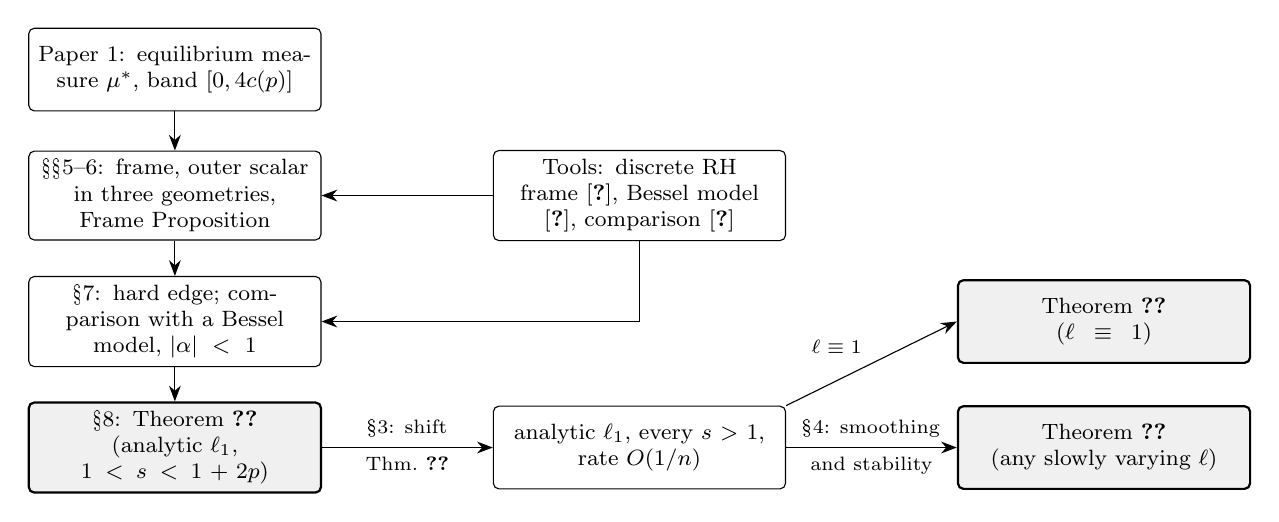
\begin{tikzpicture}[
  box/.style={draw,rounded corners=2pt,align=center,font=\footnotesize,inner sep=3pt,text width=3.5cm,
    minimum height=1.05cm},
  res/.style={box,fill=black!6,thick},
  arr/.style={-{Stealth[length=2mm]}},
  lab/.style={font=\scriptsize,align=center}]
  \node[box] (P1) at (0,0) {Paper 1: equilibrium measure $\mu^*$, band $[0,4c(p)]$};
  \node[box] (FR) at (0,-1.6) {\S\S5--6: frame, outer scalar in three geometries, Frame Proposition};
  \node[box] (HE) at (0,-3.2) {\S7: hard edge; comparison with a Bessel model, $|\alpha|<1$};
  \node[res] (T4) at (0,-4.8) {\S8: Theorem~\ref{thm:engine}\\ (analytic $\ell_1$, $1<s<1+2p$)};
  \node[box] (TL) at (5.9,-1.6) {Tools: discrete RH frame \cite{WLXZ}, Bessel model \cite{KMVV}, comparison \cite{CD}};
  \node[box] (AN) at (5.9,-4.8) {analytic $\ell_1$, every $s>1$,\\ rate $O(1/n)$};
  \node[res] (T2) at (11.8,-3.2) {Theorem~\ref{thm:pure}\\ ($\ell\equiv1$)};
  \node[res] (T1) at (11.8,-4.8) {Theorem~\ref{thm:main}\\ (any slowly varying $\ell$)};
  \draw[arr] (P1) -- (FR);
  \draw[arr] (FR) -- (HE);
  \draw[arr] (HE) -- (T4);
  \draw[arr] (TL) -- (FR);
  \draw[arr] (TL.south) |- (HE.east);
  \draw[arr] (T4) -- node[lab,above]{\S3: shift} node[lab,below]{Thm.~\ref{thm:shift}} (AN);
  \draw[arr] (AN) -- node[lab,above]{\S4: smoothing} node[lab,below]{and stability} (T1);
  \draw[arr] (AN.north east) -- node[lab,above left]{$\ell\equiv1$} (T2.west);
\end{tikzpicture}
\caption{Structure of the proof. Sections~\ref{sec:shift} and~\ref{sec:smoothing} are elementary and reduce
Theorems~\ref{thm:main} and~\ref{thm:pure} to Theorem~\ref{thm:engine}, which is proved in
Sections~\ref{sec:frame}--\ref{sec:extraction}.}
\label{fig:dependency}
\end{figure}

\subsection{Organisation}\label{sec:organisation}
Section~\ref{sec:prelim} fixes conventions, proves two facts about slowly varying sequences, quotes the input from
\cite{Paper1} (only parts (i) and (ii) of its Theorem~1.3 are used), and states the external tools with their
hypotheses. Section~\ref{sec:shift} proves Theorem~\ref{thm:shift}. Section~\ref{sec:smoothing} reduces arbitrary
slowly varying factors to analytic ones and proves Theorems~\ref{thm:main} and~\ref{thm:pure}, assuming
Theorem~\ref{thm:engine}. Sections~\ref{sec:frame}--\ref{sec:extraction} prove Theorem~\ref{thm:engine}: the common
frame (Section~\ref{sec:frame}), the outer scalar function in the three geometries $p>1$, $p=1$ and $p<1$
(Section~\ref{sec:outer}), the comparison at the hard edge (Section~\ref{sec:hardedge}), and the extraction of $a_n$ and
$b_n$ (Section~\ref{sec:extraction}). Section~\ref{sec:numerics} illustrates the results numerically, and
Section~\ref{sec:further} collects remarks and open problems. The appendices contain two $L^2$ bounds on a star of arcs
(Appendix~\ref{app:L2}), the proof of the uniform resolvent bound (Appendix~\ref{app:resolvent}) and the a priori bound
at the hard edge (Appendix~\ref{app:apriori}). A reader who is mainly interested in the Riemann--Hilbert analysis can
start at Section~\ref{sec:frame}, with the statement of Theorem~\ref{thm:engine} in hand.

Throughout, $p>0$ is fixed, $C,C'$ denote positive constants that may change from line to line (never $c$, which is
reserved for $c(p)$), and $n$ is the degree.

% Section 2: Preliminaries.
% Labels defined here: sec:prelim, sec:prelim-op, sec:prelim-sv, sec:prelim-rates, sec:prelim-eq, sec:tools,
%   eq:rec-monic, eq:rec-orth, eq:coef-int, eq:christoffel, eq:Kn-le-1, eq:regular-facts,
%   lem:potter, rem:lambda2, def:regular, rem:majorant, prop:equilibrium,
%   tool:T1, tool:T2, tool:T3, tool:T4, eq:Y-solution, eq:Y-extract, eq:CD-moments.
\makeatletter
\providecommand{\settoollabel}[2]{{\def\@currentlabel{#1}\phantomsection\label{#2}}}
\makeatother
\providecommand{\Cauchy}{\mathcal{C}}
\providecommand{\dC}{\partial\mathcal{C}}
\providecommand{\Res}{\operatorname*{Res}}
\providecommand{\Ath}[1]{\textup{(A$_{#1}$)}}

\section{Preliminaries}\label{sec:prelim}

This section fixes conventions and collects the inputs of the proof. Two elementary facts about slowly varying
sequences are used repeatedly: they are locally almost constant on dyadic scales, and they grow more slowly than any
power. We prove both in \S\ref{sec:prelim-sv}. The only input from the companion paper~\cite{Paper1} is the explicit
equilibrium measure (\S\ref{sec:prelim-eq}). Every external result used later is stated in \S\ref{sec:tools}, with its
hypotheses, under a label \ref{tool:T1}--\ref{tool:T4} by which the later sections refer to it.

\emph{Notation used throughout.} The data are $p>0$, $s>1$ and $\ell$ (\S\ref{sec:setting}); $\osc_n(\lambda)$,
$\Lambda$, $\varepsilon_\Lambda$, \Ath{\vartheta}, $L_\ell$, $G$, $\Lambda_\ell$, $\rho_\ell$ and the
regular rates $\eta_n$ are defined in \S\ref{sec:results}; the head margin $M_0$ in \S\ref{sec:smoothing-stab}. In
Sections~\ref{sec:frame}--\ref{sec:extraction} and the appendices the exponent $s$ lies in the window $(1,1+2p)$, the
analytic factor is $\ell_1=e^{\Lambda(\log\cdot)}$, and $\alpha=(s-1-p)/p\in(-1,1)$ is the Bessel order of the hard edge;
the Riemann--Hilbert notation is introduced in \S\S\ref{sec:frame-standing}--\ref{sec:frame-transf} (the chain of
matrices $Y\to U\to R\to T\to S\to V\to Q$ is displayed at the start of Section~\ref{sec:frame}), and
Table~\ref{tab:geometry} lists the quantities that depend on whether $p>1$, $p=1$ or $p<1$. Symbols used only inside
one proof are local to it.

\subsection{Orthogonal polynomials and Jacobi coefficients}\label{sec:prelim-op}

Let $\sigma$ be a positive Borel measure on $[0,\infty)$ with infinite support and finite moments. Its Hankel
determinants are positive, so the monic orthogonal polynomials $P_n$ ($\deg P_n=n$) exist for every $n\ge0$. Put
$h_n:=\int P_n^2\diff\sigma>0$, $P_{-1}:=0$ and $b_0:=0$. The polynomials satisfy the three-term recurrence
\begin{equation}\label{eq:rec-monic}
  xP_n=P_{n+1}+a_nP_n+b_n^2P_{n-1}\qquad(n\ge0),\qquad b_n^2=\frac{h_n}{h_{n-1}}\quad(n\ge1),
\end{equation}
with $a_n\in\R$ and $b_n>0$ for $n\ge1$. We call $a_n$ and $b_n$ the \emph{Jacobi coefficients} of $\sigma$.%
\footnote{The companion paper~\cite{Paper1} writes $xP_k=P_{k+1}+a_{k+1}P_k+b_k^2P_{k-1}$; its $a_{n+1}$ is our $a_n$, and $b_n$
agrees.}
Multiplying $\sigma$ by a positive constant does not change them.

The orthonormal polynomials $p_n:=P_n/\sqrt{h_n}$ satisfy
\begin{equation}\label{eq:rec-orth}
  xp_n=b_{n+1}p_{n+1}+a_np_n+b_np_{n-1}\qquad(n\ge0),
\end{equation}
as one sees by dividing \eqref{eq:rec-monic} by $\sqrt{h_n}$ and using $b_n^2\sqrt{h_{n-1}/h_n}=b_n$. Since $xp_j$ has
degree $j+1$, orthonormality gives
\begin{equation}\label{eq:coef-int}
  a_n=\int xp_n^2\diff\sigma,\qquad b_n=\int xp_{n-1}p_n\diff\sigma,\qquad \int xp_np_j\diff\sigma=0\quad(j\le n-2).
\end{equation}
In matrix form, \eqref{eq:rec-orth} says that the symmetric tridiagonal matrix $\mathcal J(\sigma)$ with diagonal
$(a_0,a_1,\dots)$ and off-diagonal $(b_1,b_2,\dots)$ is the Jacobi matrix of $\sigma$. The monic form
\eqref{eq:rec-monic} corresponds to the non-symmetric matrix $J=J(\sigma)$ with $J_{n,n}=a_n$, $J_{n,n+1}=1$ and
$J_{n+1,n}=b_{n+1}^2$; this is the form used in Section~\ref{sec:shift}.

\emph{Christoffel's extremal property.} For $y\in\R$ and $m\ge1$ let $\mathsf K_m(y):=\sum_{j<m}p_j(y)^2$. If $\deg P<m$,
then $P=\sum_{j<m}\langle P,p_j\rangle p_j$ with $\langle P,p_j\rangle:=\int Pp_j\diff\sigma$, and the Cauchy--Schwarz
inequality gives $P(y)^2\le\mathsf K_m(y)\sum_j\langle P,p_j\rangle^2=\mathsf K_m(y)\int P^2\diff\sigma$, with equality
for $\langle P,p_j\rangle=p_j(y)$. Hence
\begin{equation}\label{eq:christoffel}
  \frac1{\mathsf K_m(y)}=\min\Bigl\{\int P^2\diff\sigma:\ \deg P<m,\ P(y)=1\Bigr\}.
\end{equation}
If $\sigma$ has an atom of mass $w$ at $y$, then every competitor in \eqref{eq:christoffel} has
$\int P^2\diff\sigma\ge wP(y)^2=w$, and therefore
\begin{equation}\label{eq:Kn-le-1}
  w\,\mathsf K_m(y)\le1 .
\end{equation}

\subsection{Slow variation}\label{sec:prelim-sv}

Let $\ell$ be slowly varying (Definition~\ref{def:sv}). Each $\osc_n(\lambda)$ is a maximum of finitely many finite numbers. Put
\[
  \osc^*_n:=\sup_{m\ge n}\osc_m(2).
\]
Since $\osc_m(2)\to0$, every $\osc^*_n$ is finite, the sequence $(\osc^*_n)$ is non-increasing, and
$\osc^*_n\to0$.

\begin{lemma}[Dyadic chaining and Potter bounds]\label{lem:potter}
Let $\ell$ be slowly varying.
\begin{enumerate}
\item[\textup{(i)}] For all $n\ge1$ and all integers $k\ge n$,
  $|\log\ell(k)-\log\ell(n)|\le\osc^*_n\bigl(1+\log_2(k/n)\bigr)$.
\item[\textup{(ii)}] For every $\eta>0$ there is $A_\eta<\infty$ such that $e^{-A_\eta}k^{-\eta}\le\ell(k)\le e^{A_\eta}k^{\eta}$ for
  all $k\ge1$.
\end{enumerate}
\end{lemma}

\begin{proof}
(i) Let $j:=\lfloor\log_2(k/n)\rfloor\ge0$, so that $2^jn\le k<2^{j+1}n$. For $0\le i<j$ the integer $2^{i+1}n$ lies in
$[2^in/2,\,2\cdot2^in]$, so $|\log\ell(2^{i+1}n)-\log\ell(2^in)|\le\osc_{2^in}(2)\le\osc^*_n$. Also $k\in[2^jn,\,2\cdot
2^jn]$, so $|\log\ell(k)-\log\ell(2^jn)|\le\osc^*_n$. Summing these $j+1$ steps ($j$ dyadic steps and one final
step) gives
$|\log\ell(k)-\log\ell(n)|\le(j+1)\osc^*_n\le\osc^*_n(1+\log_2(k/n))$.

(ii) Fix $\eta>0$ and choose $m$ with $\osc^*_m\le\eta\log2$. For $k\ge m$, part (i) with $n=m$ gives
\[
  |\log\ell(k)|\le|\log\ell(m)|+\osc^*_m+\frac{\osc^*_m}{\log2}\log\frac km\le|\log\ell(m)|+\osc^*_m+\eta\log k .
\]
The finitely many $k<m$ are covered by taking
\[
  A_\eta:=\max\bigl(|\log\ell(m)|+\osc^*_m,\ \max_{k<m}|\log\ell(k)|\bigr).
\]
\end{proof}

\begin{remark}[$\lambda=2$ suffices]\label{rem:lambda2}
If $\osc_n(2)\to0$, then $\osc_n(\lambda)\to0$ for every $\lambda\ge1$. Indeed, Lemma~\ref{lem:potter}(i) uses only
$\osc(2)$. For $n\le k\le\lambda n$ it gives $|\log\ell(k)-\log\ell(n)|\le\osc^*_n(1+\log_2\lambda)$. For $n/\lambda\le
k<n$, apply it with base point $k$: $|\log\ell(n)-\log\ell(k)|\le\osc^*_k(1+\log_2(n/k))\le\osc^*_{\lceil
n/\lambda\rceil}(1+\log_2\lambda)$. Both bounds tend to $0$.
\end{remark}

For every $s>1$, Lemma~\ref{lem:potter}(ii) with $\eta<s-1$ gives $\sum_kk^{-s}\ell(k)<\infty$. So
$\sigma_{p,s,\ell}=\sum_kk^{-s}\ell(k)\delta_{k^{-p}}$ is a finite measure on $(0,1]$ with infinitely many atoms, and
\S\ref{sec:prelim-op} applies to it.

\subsection{Regular rates}\label{sec:prelim-rates}

\phantomsection\label{def:regular}%
Regular rates were defined before Theorem~\ref{thm:shift}. Every regular rate satisfies
\begin{equation}\label{eq:regular-facts}
  \frac1n\le\frac{\eta_n}{\eta_1},\qquad \eta_{n-1}\le2\eta_n\quad(n\ge2),\qquad \sum_n\eta_n=\infty .
\end{equation}
The first holds because $n\eta_n\ge\eta_1$; the second because $(n-1)\eta_{n-1}\le n\eta_n$; the third follows from
the first.

\begin{remark}[Regular majorants]\label{rem:majorant}
Every non-increasing sequence $\upsilon_n>0$ with $\upsilon_n\to0$ is dominated by a regular rate, namely
$\eta_n:=\max_{m\le n}(m\upsilon_m)/n$. Indeed $\eta_n\ge\upsilon_n$ and $n\eta_n$ is non-decreasing by construction;
$\eta_{n+1}\le\max\bigl(\eta_n\,n/(n+1),\upsilon_{n+1}\bigr)\le\eta_n$ because $\upsilon_{n+1}\le\upsilon_n\le\eta_n$; and
$\eta_n\to0$, since $m\upsilon_m/n\le\upsilon_1/\sqrt n$ for $m\le\sqrt n$ and $m\upsilon_m/n\le\upsilon_{\lceil\sqrt n\rceil}$
for $\sqrt n<m\le n$. So Theorem~\ref{thm:shift} applies to any monotone rate. We use it only with $\eta_n=1/n$.
\end{remark}

\subsection{The equilibrium measure}\label{sec:prelim-eq}

The Riemann--Hilbert analysis of Sections~\ref{sec:frame}--\ref{sec:extraction} is built on the equilibrium measure
of the constrained problem solved in~\cite{Paper1}. We use only its explicit form and the equality of its potential on the band; the optimality
statement \cite[Theorem~1.3(iii)]{Paper1} is not used anywhere in this paper.

Let $c=c(p)$ and $I(p)$ be as in \eqref{eq:cp}, let $\gamma_p:=\log c(p)+p$, and let $\lambda_p(x):=\frac1px^{-1-1/p}$ be the density
of the nodes $k^{-p}$ (the image of Lebesgue measure on $(0,\infty)$ under $u\mapsto u^{-p}$). For $V\in[0,1]$ and
$a,b>0$ write $\mathcal I_V(a,b):=B(a,b)^{-1}\int_0^Vt^{a-1}(1-t)^{b-1}\diff t$ for the regularised incomplete beta
function ($B$ is Euler's Beta function). For $\beta>0$ let $\mathrm{arc}_\beta$ be the arcsine law on $[0,\beta]$, with
density $1/(\pi\sqrt{y(\beta-y)})$, and put $\beta_\tau:=4c\tau^{-p}$ for $0<\tau\le1$.

\begin{proposition}[{\cite[Theorem~1.3(i)--(ii)]{Paper1}}]\label{prop:equilibrium}
Let $p>0$ and let $\mu^*:=\int_0^1\mathrm{arc}_{\beta_\tau}\diff\tau$, a probability measure on $(0,\infty)$.
\begin{enumerate}
\item[\textup{(i)}] $\mu^*$ has the density
  \[
    \psi^*(x)=\lambda_p(x)\,\mathcal I_{\min(1,\,x/4c)}\bigl(\tfrac1p+\tfrac12,\tfrac12\bigr),\qquad x>0 .
  \]
  In particular $\psi^*=\lambda_p$ on $[4c,\infty)$ (saturation) and $0<\psi^*<\lambda_p$ on $(0,4c)$.
\item[\textup{(ii)}] The function $U^*(x):=\int\log|x-y|\diff\mu^*(y)$ satisfies $U^*(x)=\gamma_p$ for $0<x\le4c$, and
  $U^*(x)\ge\gamma_p$ for all $x>0$.
\item[\textup{(iii)}] (Hard edge.) As $x\to0^+$,
  \[
    \psi^*(x)=C_*x^{-1/2}\bigl(1+O(x)\bigr),\qquad C_*:=\frac{(4c)^{-1/p-1/2}}{p\,a_*B(a_*,\frac12)},\quad
    a_*:=\frac1p+\frac12 .
  \]
\end{enumerate}
\end{proposition}

\begin{proof}
Parts (i) and (ii) are \cite[Theorem~1.3(i)--(ii)]{Paper1}, transported from the variable $u$ to $x=u^{-p}$: there,
$\mu^*_u$ is the image of $\mu^*$ under $x\mapsto x^{-1/p}$ and has density
$\rho^*(u)=\mathcal I_{\min(1,u^{-p}/4c)}(\frac1p+\frac12,\frac12)$, with $\rho^*=1$ exactly on $(0,(4c)^{-1/p}]$ and
$0<\rho^*<1$ on $((4c)^{-1/p},\infty)$. Since $|\diff u/\diff x|=\lambda_p(x)$, the density of $\mu^*$ in $x$ is
$\lambda_p(x)\rho^*(x^{-1/p})$, which is (i). Part (ii) is quoted verbatim, with $\gamma_p=\log c+p$. For (iii), let
$V=x/4c\le1$. Then $\int_0^Vt^{a_*-1}(1-t)^{-1/2}\diff t=\frac{V^{a_*}}{a_*}(1+O(V))$, so
$\psi^*(x)=\frac1px^{-1-1/p}(x/4c)^{1/p+1/2}\bigl(a_*B(a_*,\frac12)\bigr)^{-1}(1+O(x))$, which is (iii).
\end{proof}

The point $x=4c$ is the soft edge, $(0,4c)$ is the band, and $x=0$ is the hard edge, where $\mu^*$ has the
inverse-square-root density of (iii).

\subsection{Tools}\label{sec:tools}

This subsection states every external result used in Sections~\ref{sec:frame}--\ref{sec:extraction} and the
appendices, with its hypotheses and the equation numbers of the source; the later sections refer to the items as
\ref{tool:T1}--\ref{tool:T4}. It is needed only from Section~\ref{sec:frame} on, and a reader may skip it until then.
Throughout, the Cauchy transform on an oriented contour $\Sigma$ is
\[
  \Cauchy f(z):=\frac1{2\pi i}\int_\Sigma\frac{f(s)\diff s}{s-z},\qquad z\in\C\setminus\Sigma,
\]
and $\Cauchy_\pm f$ are its non-tangential boundary values from the left ($+$) and the right ($-$) of $\Sigma$, so that
$\Cauchy_+-\Cauchy_-=1$. For a jump matrix $v$ on $\Sigma$ we write $\Cauchy_vf:=\Cauchy_-\bigl(f(v-I)\bigr)$. Matrices
$\sigma_1,\sigma_2,\sigma_3$ are the Pauli matrices, and $\sigma_3=\mathrm{diag}(1,-1)$.

\medskip
\noindent\textbf{T1. The discrete interpolation problem
(Wu--Lin--Xu--Zhao~\cite{WLXZ}).}\settoollabel{T1}{tool:T1}
Wu, Lin, Xu and Zhao~\cite{WLXZ} develop the Riemann--Hilbert method for discrete orthogonal polynomials on infinitely
many nodes with an accumulation point, for the Tricomi--Carlitz polynomials. We apply none of their theorems to our
measures; we use the formulation of the problem and the order of the transformations, and our versions are written out
in Sections~\ref{sec:frame} and~\ref{sec:outer}.

\emph{(a) The problem and its solution.} Let $\sigma=\sum_{k\ge1}w_k\delta_{x_k}$ with distinct nodes
$x_k\in(0,1]$, $w_k>0$ and $\sum_kw_k<\infty$, and fix $n\ge1$. Following \cite[(2.14) and Theorem~2.3]{WLXZ}, put
\begin{equation}\label{eq:Y-solution}
  Y(z):=\begin{pmatrix}P_n(z) & \displaystyle\sum_k\frac{w_kP_n(x_k)}{z-x_k}\\[3mm]
  h_{n-1}^{-1}P_{n-1}(z) & \displaystyle h_{n-1}^{-1}\sum_k\frac{w_kP_{n-1}(x_k)}{z-x_k}\end{pmatrix}.
\end{equation}
Then $Y$ is analytic in $\C\setminus(\{x_k\}_k\cup\{0\})$; at each node it has a simple pole with
$\Res_{z=x_k}Y(z)=\lim_{z\to x_k}Y(z)\bigl(\begin{smallmatrix}0&w_k\\0&0\end{smallmatrix}\bigr)$ (the residue
condition \cite[(2.14)]{WLXZ}); and $Y(z)z^{-n\sigma_3}=I+Y_1/z+Y_2/z^2+O(z^{-3})$ as $z\to\infty$, with
\begin{equation}\label{eq:Y-extract}
  (Y_1)_{12}(Y_1)_{21}=b_n^2,\qquad \frac{(Y_2)_{12}}{(Y_1)_{12}}-(Y_1)_{22}=a_n .
\end{equation}
\emph{Proof.} The sums converge locally uniformly off $\{x_k\}\cup\{0\}$, which gives analyticity, the simple poles and
$\Res_{x_k}Y_{j2}=w_kY_{j1}(x_k)$. Write $P_m(x)=x^m+\pi_mx^{m-1}+\dots$. For $|z|>2$, expanding $(z-x)^{-1}$ gives
$\sum_kw_kP_m(x_k)/(z-x_k)=\sum_{i\ge0}z^{-i-1}\int P_mx^i\diff\sigma$, and $\int P_mx^i\diff\sigma$ equals $0$ for $i<m$,
$h_m$ for $i=m$ and $-\pi_{m+1}h_m$ for $i=m+1$. Hence $(Y_1)_{12}=h_n$, $(Y_1)_{21}=h_{n-1}^{-1}$,
$(Y_2)_{12}=-\pi_{n+1}h_n$ and $(Y_1)_{22}=-\pi_n$; and $\pi_n=\pi_{n+1}+a_n$ by \eqref{eq:rec-monic}. \qed

\emph{(b) Transformations.} The transformations of Section~\ref{sec:frame} follow \cite[\S\S3--5]{WLXZ}: removal of the
poles by triangular factors built from $\Pi=\sin\theta/\theta'$ and $e^{\pm i\theta}$ \cite[(3.9)--(3.15)]{WLXZ},
normalisation by the $g$-function \cite[(4.1)]{WLXZ}, the lens and saturated-region factors $V_\pm$, $V^\triangle_\pm$
\cite[(4.12)--(4.13)]{WLXZ}, and conjugation by an outer scalar \cite[(5.1)]{WLXZ}. In \cite{WLXZ} these are written in
a symmetric variable with nodes $\pm x_k$; we use only the pattern, and every jump is recomputed in
Section~\ref{sec:frame} for our one-sided problem.

\emph{(c) The soft edge.} Our Airy parametrix (Lemma~\ref{lem:airy}) follows the pattern of \cite[\S6.1,
(6.4), (6.10)--(6.12)]{WLXZ}; it is constructed from the Airy function directly (\ref{tool:T4}), and no statement of
\cite{WLXZ} is used.

\medskip
\noindent\textbf{T2. The Bessel model problem (Kuijlaars, McLaughlin, Van Assche and Vanlessen~\cite{KMVV}).}%
\settoollabel{T2}{tool:T2}
We use the explicit Bessel model of \cite[\S6]{KMVV} and its algebraic properties; we apply none of their theorems on
orthogonal polynomials, so their standing hypothesis on the weight \cite[(1.1)]{KMVV} plays no role.

\emph{(a) The model.} Let $\alpha>-1$ and let $\Sigma_\Psi$ consist of the rays $\gamma_1:\arg\zeta=2\pi/3$,
$\gamma_2:\arg\zeta=\pi$ and $\gamma_3:\arg\zeta=-2\pi/3$, all oriented towards the origin, with the $+$ side on the
left \cite[Figure~3]{KMVV}. The function
\[
  \Psi_\alpha(\zeta)=\begin{pmatrix}I_\alpha(2\zeta^{1/2}) & \frac i\pi K_\alpha(2\zeta^{1/2})\\[1mm]
  2\pi i\zeta^{1/2}I_\alpha'(2\zeta^{1/2}) & -2\zeta^{1/2}K_\alpha'(2\zeta^{1/2})\end{pmatrix},\qquad|\arg\zeta|<2\pi/3
\]
\cite[(6.23)]{KMVV}, continued to $2\pi/3<\pm\arg\zeta<\pi$ by the Hankel-function formulas \cite[(6.24)--(6.25)]{KMVV},
solves the Bessel model problem \cite[Theorem~6.3]{KMVV}, with jumps
\[
  \begin{pmatrix}1&0\\e^{\alpha\pi i}&1\end{pmatrix}\ \text{on }\gamma_1,\qquad
  \begin{pmatrix}0&1\\-1&0\end{pmatrix}\ \text{on }\gamma_2,\qquad
  \begin{pmatrix}1&0\\e^{-\alpha\pi i}&1\end{pmatrix}\ \text{on }\gamma_3
\]
\cite[(6.16)--(6.18)]{KMVV}. Uniformly as $\zeta\to\infty$ in $\C\setminus\Sigma_\Psi$,
\[
  \Psi_\alpha(\zeta)=(2\pi\zeta^{1/2})^{-\sigma_3/2}\frac1{\sqrt2}
  \begin{pmatrix}1+O(\zeta^{-1/2})&i+O(\zeta^{-1/2})\\ i+O(\zeta^{-1/2})&1+O(\zeta^{-1/2})\end{pmatrix}e^{2\zeta^{1/2}\sigma_3}
\]
\cite[(6.28)]{KMVV}, which follows from the large-argument expansions (\ref{tool:T4}) of the Bessel and Hankel
functions in (6.23)--(6.25); this also covers the rays moved by (b) (\S\ref{sec:he-model}).

\emph{(b) Angle freedom.} By the remark after \cite[(6.21)]{KMVV}, the angle $2\pi/3$ may be replaced by any angle in
$(0,\pi)$; the lens contours in the disc are then the preimages of the rays under $\zeta=n^2f(z)$, and they do not
depend on $n$. We use rays at $\pm(\pi-\vartheta_{\mathrm{lip}})$.

\emph{(c) The left endpoint.} Our hard edge has the band to its right, as the endpoint $-1$ of \cite{KMVV}. There the
conformal map reverses orientation, and the reversal is absorbed by conjugation with $\sigma_3$:
$\tilde\Psi(\zeta)=\sigma_3\Psi(\zeta;\alpha\to\beta)\sigma_3$ \cite[(6.51)]{KMVV}, with prefactor
\[
  \tilde E_n(z)=N(z)\tilde W(z)^{\sigma_3}\tfrac1{\sqrt2}\begin{pmatrix}1&i\\i&1\end{pmatrix}
  \tilde f(z)^{\sigma_3/4}(2\pi n)^{\sigma_3/2}
\]
\cite[(6.53)]{KMVV}, where $N$, $\tilde W$ and $\tilde f$ are the global parametrix, an analytic square root of the
weight and the local conformal map of \cite{KMVV} (compare the right-endpoint formulas
\cite[(6.27), (6.31)]{KMVV} and $\det E_n\equiv1$ \cite[(6.33)]{KMVV}). The prefactor is analytic by removability: its
entries have at most a square-root singularity at the endpoint and it is analytic in a punctured neighbourhood
\cite[proof of Proposition~6.5]{KMVV}. In Section~\ref{sec:hardedge} this argument is applied only to a prefactor
that does not involve the weight.

\medskip
\noindent\textbf{T3. The comparison argument (Conway--Deift~\cite{CD}).}\settoollabel{T3}{tool:T3}
The following are from \cite[\S4]{CD}, whose Cauchy operator is normalised as ours. Lebesgue exponents are written
$r,r'$ (\cite{CD} writes $p,q$).

\emph{(a) Boundedness and the class $\dC$} \cite[\S4.1]{CD}. $\Cauchy_\pm$ are bounded on $L^2(\Sigma)$ (and on
$L^r(\Sigma)$, $1<r<\infty$) if and only if $\Sigma$ is Carleson. A pair $A_\pm\in L^r(\Sigma)$ belongs to
$\dC(L^r(\Sigma))$ if $A_\pm=\Cauchy_\pm f$ for some (unique) $f\in L^r(\Sigma)$; we write $A_\pm\in I+\dC(L^r)$ if
$A_\pm-I\in\dC(L^r)$.

\emph{(b) Theorem~4.4 of \cite{CD}.} \emph{Let $v_A,v_B\in L^\infty(\Sigma)$ with $v_B^{-1}\in L^\infty(\Sigma)$. Let
$A_\pm\in I+\dC(L^r(\Sigma))$ satisfy $A_+=A_-v_A$ on $\Sigma$, and let $B_\pm\in I+\dC(L^r(\Sigma))$ satisfy
$B_+=B_-v_B$ on $\Sigma$, with $B_\pm^{-1}\in I+\dC(L^{r'}(\Sigma))$, $1/r+1/r'=1$. If $A,B$ are the analytic
extensions of $A_\pm,B_\pm$, then}
\[
  AB^{-1}=I+\Cauchy\bigl(A_-(v_Av_B^{-1}-I)B_-^{-1}\bigr).
\]
\emph{Consequence (moments at infinity).} If in addition $\Sigma$ is bounded and $A=I+A_1/z+A_2/z^2+O(z^{-3})$,
$B=I+B_1/z+B_2/z^2+O(z^{-3})$ as $z\to\infty$, then with $\mathcal E:=A_-(v_A-v_B)v_B^{-1}B_-^{-1}\in L^1(\Sigma)$
(take $r=r'=2$),
\begin{equation}\label{eq:CD-moments}
  A_1-B_1=-\frac1{2\pi i}\int_\Sigma\mathcal E(s)\diff s,\qquad
  A_2-B_2=-\frac1{2\pi i}\int_\Sigma s\mathcal E(s)\diff s+(A_1-B_1)B_1 .
\end{equation}
Indeed $v_Av_B^{-1}-I=(v_A-v_B)v_B^{-1}$; for $|z|>\max_\Sigma|s|$ expand $1/(s-z)=-\sum_{j\ge0}s^jz^{-j-1}$ in
$\Cauchy\mathcal E(z)$ and compare with $AB^{-1}=I+(A_1-B_1)z^{-1}+\bigl(A_2-B_2-(A_1-B_1)B_1\bigr)z^{-2}+O(z^{-3})$.
This is the mechanism of \cite[Proposition~4.9]{CD}, whose proof identifies $\mu=Q_-$ and
$\tilde\mu=\tilde Q_-$. Formula (4.14) of \cite{CD} is printed without the factor $v_B^{-1}$; it agrees with
\eqref{eq:CD-moments} when $(v_A-v_B)v_B^{-1}=v_A-v_B$, as in their setting. We use the form derived from
Theorem~4.4.

\emph{(c) Solution formula} \cite[\S4.2]{CD}. If $1-\Cauchy_{v}$ is invertible on $L^2(\Sigma)$, then
$\mu:=(1-\Cauchy_v)^{-1}I$ gives the unique solution $X(z)=I+\Cauchy(\mu(v-I))(z)$ of the RH problem normalised at
infinity with jump $v$.

\emph{(d) The Neumann-series step} \cite[proof of Theorem~4.7, (4.12)--(4.13)]{CD}. If
$\|(1-\Cauchy_{\tilde v})^{-1}\|_{L^2\to L^2}\le K$ and $\|\Cauchy_v-\Cauchy_{\tilde v}\|_{L^2\to L^2}\le1/(2K)$, then
\[
  (1-\Cauchy_v)^{-1}=(1-\Cauchy_{\tilde v})^{-1}\bigl(1-(\Cauchy_v-\Cauchy_{\tilde v})(1-\Cauchy_{\tilde v})^{-1}\bigr)^{-1}
\]
exists and has norm at most $2K$, since the inner factor is $1$ minus an operator of norm at most $\frac12$. In
\cite{CD} the smallness comes from $\|v-\tilde v\|_{L^\infty(\Sigma)}\to0$.

\emph{(e) Proposition~4.6 of \cite{CD}} (attributed there to Deift and Zhou). The operators $(1-\Cauchy_{h_n})^{-1}$
are bounded uniformly in $n$ if and only if the inhomogeneous problem $m_+=m_-h_n+g$ on $\Sigma$,
$m_\pm\in\dC(L^2(\Sigma))$, is uniquely solvable for every $g\in L^2(\Sigma)$ with $\|m_\pm\|_{L^2}\le C\|g\|_{L^2}$, $C$
independent of $n$ and $g$. We use only the direction ``solvable with bounds $\Rightarrow$ bounded inverse'', and we
re-prove it in Appendix~\ref{app:resolvent}.

We do \emph{not} use \cite[Theorem~4.5]{CD}, whose proof is specific to the Legendre comparison problem.

\medskip
\noindent\textbf{T4. Special functions (NIST DLMF~\cite{DLMF}).}\settoollabel{T4}{tool:T4}
Principal branches throughout. ``Uniformly in closed subsectors'' of a sector means uniformly in every closed sector
contained in it.
\begin{itemize}
\item \emph{Gamma function.} (5.5.1) $\Gamma(z+1)=z\Gamma(z)$; (5.5.3) $\Gamma(z)\Gamma(1-z)=\pi/\sin(\pi z)$,
  $z\notin\mathbb Z$; (5.11.1) $\mathrm{Ln}\,\Gamma(z)\sim(z-\frac12)\ln z-z+\frac12\ln(2\pi)+\sum_{k\ge1}
  \frac{B_{2k}}{2k(2k-1)z^{2k-1}}$ as $z\to\infty$, uniformly in closed subsectors of $|\mathrm{ph}\,z|<\pi$, where by
  \S5.11(ii) the remainder after the term $k=m-1$ is at most $\sec^{2m}(\frac12\mathrm{ph}\,z)$ times the first
  neglected term; (5.12.3), (5.12.1) $\int_0^\infty t^{a-1}(1+t)^{-a-b}\diff t=B(a,b)=\Gamma(a)\Gamma(b)/\Gamma(a+b)$ for $\Re a,\Re b>0$.
\item \emph{Airy functions} (\S\S9.2, 9.7). $\mathrm{Ai}$ is entire, and $\mathrm{Ai}(z)$, $\mathrm{Ai}(ze^{\mp2\pi i/3})$
  solve $w''=zw$; (9.2.8) $\mathcal W\{\mathrm{Ai}(z),\mathrm{Ai}(ze^{\mp2\pi i/3})\}=e^{\pm\pi i/6}/(2\pi)$; (9.2.12)
  $\mathrm{Ai}(z)+e^{-2\pi i/3}\mathrm{Ai}(ze^{-2\pi i/3})+e^{2\pi i/3}\mathrm{Ai}(ze^{2\pi i/3})=0$. By (9.7.5)--(9.7.6),
  with $u_0=v_0=1$ (9.7.2), as $z\to\infty$ uniformly in closed subsectors of $|\mathrm{ph}\,z|<\pi$,
  \[
    \mathrm{Ai}(z)=\frac{e^{-\frac23z^{3/2}}}{2\sqrt\pi\,z^{1/4}}\bigl(1+O(|z|^{-3/2})\bigr),\qquad
    \mathrm{Ai}'(z)=-\frac{z^{1/4}e^{-\frac23z^{3/2}}}{2\sqrt\pi}\bigl(1+O(|z|^{-3/2})\bigr).
  \]
\item \emph{Modified Bessel functions.} (10.25.2)
  $I_\nu(z)=(\frac12z)^\nu\sum_{k\ge0}(\frac14z^2)^k/(k!\,\Gamma(\nu+k+1))$, analytic in $\C\setminus(-\infty,0]$
  (\S10.25(ii)); (10.27.4) $K_\nu=\frac12\pi(I_{-\nu}-I_\nu)/\sin(\nu\pi)$; (10.31.2)
  $K_0(z)=-(\ln(\frac12z)+\gamma_{\mathrm E})I_0(z)+\frac14z^2+\dotsb$, $\gamma_{\mathrm E}$ being Euler's constant and the
  dots an entire function of $z^2$; (10.28.2) $\mathcal W\{K_\nu,I_\nu\}(z)=1/z$, which with (6.23) of \ref{tool:T2}
  gives $\det\Psi_\alpha=1$.
\item \emph{Large argument} (\S10.40(i), $\nu$ fixed). Let $\mathsf s_\pm(z):=\sum_k(\pm1)^ka_k(\nu)z^{-k}$,
  where $a_0(\nu)=1$ by (10.17.1). The expansions (10.40.1), (10.40.2) and (10.40.5) read
  \begin{align*}
    I_\nu(z)&\sim e^z(2\pi z)^{-1/2}\mathsf s_-(z),&&|\mathrm{ph}\,z|<\tfrac12\pi,\\
    K_\nu(z)&\sim(\pi/2z)^{1/2}e^{-z}\mathsf s_+(z),&&|\mathrm{ph}\,z|<\tfrac32\pi,\\
    I_\nu(z)&\sim(2\pi z)^{-1/2}\bigl(e^z\mathsf s_-(z)\pm ie^{\pm\nu\pi i}e^{-z}\mathsf s_+(z)\bigr),
      &&-\tfrac12\pi<\pm\mathrm{ph}\,z<\tfrac32\pi,
  \end{align*}
  uniformly in closed subsectors; and (10.40.3)--(10.40.4) are the expansions of $I_\nu',K_\nu'$ in the sectors of
  (10.40.1)--(10.40.2), with $b_k(\nu)$ in place of $a_k(\nu)$ and an overall minus sign for $K_\nu'$.
\end{itemize}

% Section 3: The Christoffel shift.
% Labels defined here: sec:shift, lem:zeros, lem:transfer, lem:chain-limit, lem:chain-rate, rem:sharp,
%   rem:converse, eq:shift-identity, eq:transfer, eq:scaled-chain, eq:chain-map.

\section{The Christoffel shift}\label{sec:shift}

Multiplying the measure by $x$ shifts the exponent $s$ by exactly $p$: for $x_k=k^{-p}$,
\begin{equation}\label{eq:shift-identity}
  x\,\sigma_{p,s,\ell}=\sum_{k\ge1}k^{-p}\,k^{-s}\ell(k)\,\delta_{k^{-p}}=\sigma_{p,s+p,\ell},
\end{equation}
with the same $\ell$. This section proves Theorem~\ref{thm:shift}: the pointwise law, with its rate, passes from
$\sigma$ to $x\sigma$. The Jacobi matrix of $x\sigma$ is obtained by factoring the Jacobi matrix of $\sigma$ as a product
$LU$ of bidiagonal matrices and multiplying the factors in the opposite order. The entries of the factors are not
known in advance, since they involve the values $P_n(0)$. The point of the section is that no information about
$P_n(0)$ is needed beyond its sign: the factors satisfy a recursion whose limiting map has a double (parabolic) fixed
point, and positivity alone forces them to converge to it.

Throughout, $a_n,b_n$ are the Jacobi coefficients of $\sigma$ (\S\ref{sec:prelim-op}), and $\tilde a_n,\tilde b_n$
are those of $x\sigma$, where $\diff(x\sigma):=x\diff\sigma(x)$. Theorem~\ref{thm:shift} states that
$|n^pa_n-2c|+|n^pb_n-c|=O(\eta_n)$ implies $|n^p\tilde a_n-2c|+|n^p\tilde b_n-c|=O(\eta_n)$ for every regular rate
$\eta_n$, and similarly without a rate.

\subsection{The transfer formulas}

\begin{lemma}\label{lem:zeros}
Let $\sigma$ be a positive Borel measure on $[0,\infty)$ with infinite support and finite moments. Then for $n\ge1$ the
polynomial $P_n$ has $n$ simple zeros, all in $(0,\infty)$. In particular $(-1)^nP_n(0)>0$ for all $n\ge0$.
\end{lemma}

\begin{proof}
Let $y_1<\dots<y_m$ be the zeros of $P_n$ in $(0,\infty)$ of odd multiplicity, and put $\pi(x):=\prod_j(x-y_j)$
($\pi:=1$ if $m=0$). Suppose $m<n$. Then $\int P_n\pi\diff\sigma=0$ by orthogonality. On the other hand, every
remaining factor of $P_n$ is of the form $(x-y)^{2i}$ with $y$ real, or $(x-y)$ with $y\le0$, or
$(x-z)(x-\bar z)=|x-z|^2$ with $z\notin\R$; each is non-negative on $[0,\infty)$. Hence $P_n\pi\ge0$ on $[0,\infty)$.
Since $P_n\pi$ is a non-zero polynomial and $\sigma$ has infinite support, $\int P_n\pi\diff\sigma>0$, a contradiction.
So $m=n$, the $n$ zeros are simple and positive, and $P_n(0)=\prod_j(-y_j)$ has the sign $(-1)^n$.
\end{proof}

By Lemma~\ref{lem:zeros} we may define
\[
  u_n:=-\frac{P_{n+1}(0)}{P_n(0)}>0\quad(n\ge0),\qquad l_0:=0,\qquad l_n:=\frac{b_n^2}{u_{n-1}}>0\quad(n\ge1).
\]

\begin{lemma}\label{lem:transfer}
Let $\sigma$ be as in Lemma~\ref{lem:zeros}. Then:
\begin{enumerate}
\item[\textup{(i)}] $a_n=u_n+l_n$ for $n\ge0$, and $b_n^2=u_{n-1}l_n$ for $n\ge1$. Equivalently, $u_0=a_0$ and
  $u_n=a_n-b_n^2/u_{n-1}$ for $n\ge1$.
\item[\textup{(ii)}] The measure $x\sigma$ has infinite support, its monic orthogonal polynomials are
  $\widetilde P_n(x):=\bigl(P_{n+1}(x)+u_nP_n(x)\bigr)/x$, and its Jacobi coefficients are
  \begin{equation}\label{eq:transfer}
    \tilde a_n=u_n+l_{n+1}\quad(n\ge0),\qquad \tilde b_n^2=u_nl_n\quad(n\ge1).
  \end{equation}
\end{enumerate}
\end{lemma}

In matrix form: $J(\sigma)=LU$, with $L$ unit lower bidiagonal with subdiagonal $(l_1,l_2,\dots)$ and $U$ upper
bidiagonal with diagonal $(u_0,u_1,\dots)$ and superdiagonal $1$; and $J(x\sigma)=UL$. This is the classical Christoffel
(or Darboux) transformation; see Derevyagin--Derkach~\cite[\S1]{DD}, where it is written $J=LU\mapsto UL$. We include
the short proof. (Equivalently, the symmetric Jacobi matrix factors as $\mathcal J(\sigma)=\mathcal L\mathcal L^{\mathsf
T}$ with $\mathcal L$ lower bidiagonal, and $\mathcal J(x\sigma)=\mathcal L^{\mathsf T}\mathcal L$; this Cholesky form
leads to a second proof of the results of this section, which we do not give.)

\begin{proof}
(i) Evaluate \eqref{eq:rec-monic} at $x=0$: $0=P_{n+1}(0)+a_nP_n(0)+b_n^2P_{n-1}(0)$. Dividing by $P_n(0)\ne0$ gives
$a_n=u_n-b_n^2P_{n-1}(0)/P_n(0)=u_n+b_n^2/u_{n-1}=u_n+l_n$ for $n\ge1$, and $a_0=u_0$ since $P_{-1}=0$. The identity
$b_n^2=u_{n-1}l_n$ is the definition of $l_n$.

(ii) The support of $x\sigma$ is $\supp\sigma\setminus\{0\}$, which is infinite, and $x\sigma$ has finite moments. The
polynomial $P_{n+1}+u_nP_n$ vanishes at $0$ by the definition of $u_n$, so $\widetilde P_n$ is a monic polynomial of
degree $n$. For $j\le n-1$, $\int\widetilde P_nx^j\diff(x\sigma)=\int(P_{n+1}+u_nP_n)x^j\diff\sigma=0$. Hence the
$\widetilde P_n$ are the monic orthogonal polynomials of $x\sigma$.

Next, for $n\ge1$ the polynomial $P_n-\widetilde P_n$ has degree at most $n-1$, and for $j\le n-2$
\[
  \int(P_n-\widetilde P_n)x^j\diff(x\sigma)=\int P_nx^{j+1}\diff\sigma-\int\widetilde P_nx^j\diff(x\sigma)=0 .
\]
So $P_n-\widetilde P_n=l_n'\widetilde P_{n-1}$ for some constant $l_n'$; put $l_0':=0$, consistent with
$P_0=\widetilde P_0=1$. Then
\[
  xP_n=x\widetilde P_n+l_n'\,x\widetilde P_{n-1}=(P_{n+1}+u_nP_n)+l_n'(P_n+u_{n-1}P_{n-1}).
\]
Comparing with \eqref{eq:rec-monic} (the $P_j$ are linearly independent) gives $a_n=u_n+l_n'$ and $b_n^2=l_n'u_{n-1}$,
so $l_n'=l_n$ by (i). Finally,
\[
  x\widetilde P_n=P_{n+1}+u_nP_n=(\widetilde P_{n+1}+l_{n+1}\widetilde P_n)+u_n(\widetilde P_n+l_n\widetilde P_{n-1}),
\]
which is the recurrence of $x\sigma$ with $\tilde a_n=u_n+l_{n+1}$ and $\tilde b_n^2=u_nl_n$.
\end{proof}

\subsection{The chain sequence converges}

Assume now that $\sigma$ satisfies the pointwise law at scale $n^p$ with constant $c>0$. We work with the rescaled
quantities
\[
  \hat a_n:=n^pa_n,\quad \hat b_n:=n^pb_n,\quad \hat u_n:=n^pu_n,\quad \hat l_n:=n^pl_n,\quad
  \kappa_n:=\Bigl(\frac{n-1}n\Bigr)^p .
\]
Multiplying the identities of Lemma~\ref{lem:transfer}(i) by $n^p$, and using $n^p\cdot(n-1)^p=n^{2p}\kappa_n$, we get
\begin{equation}\label{eq:scaled-chain}
  \hat u_n+\hat l_n=\hat a_n,\qquad \hat u_{n-1}\hat l_n=\kappa_n\hat b_n^2,\qquad\text{so}\qquad
  \hat u_n=\hat a_n-\frac{\kappa_n\hat b_n^2}{\hat u_{n-1}}\qquad(n\ge1).
\end{equation}
If $\hat a_n\to2c$, $\hat b_n\to c$ and $\hat u_{n-1}\to c$, the last identity tends to
\begin{equation}\label{eq:chain-map}
  \hat u_n\approx F(\hat u_{n-1}),\qquad F(t):=2c-\frac{c^2}t,\qquad
  F(t)-t=-\frac{(t-c)^2}t,\qquad F(c+y)=c+\frac{cy}{c+y}.
\end{equation}
The map $F$ is increasing on $(0,\infty)$, has the single fixed point $c$, and this fixed point is double: $F(t)\le t$
for every $t>0$. An orbit that settles below $c$ is therefore pushed down towards $0$, and one above $c$ is pulled down
to $c$. Positivity of $u_n$ rules out the first possibility.

\begin{lemma}\label{lem:chain-limit}
Let $\sigma$ be as in Lemma~\ref{lem:zeros}, $p>0$ and $c>0$. If $\hat a_n\to2c$ and $\hat b_n\to c$, then
$\hat u_n\to c$ and $\hat l_n\to c$.
\end{lemma}

Lemma~\ref{lem:chain-limit} is a special case of Dai--Piao--Qiao~\cite[Proposition~2.1]{DPQ}: in the variables
$\mathsf a_n:=b_n^2/(a_{n-1}a_n)$ and $\mathsf m_n:=l_n/a_n$ one has $\mathsf a_n=(1-\mathsf m_{n-1})\mathsf m_n$ with
$\mathsf m_0=0$ and $0<\mathsf m_n<1$, so $(\mathsf a_n)$ is a chain sequence with parameter sequence $(\mathsf m_n)$; the
hypothesis gives $\mathsf a_n=\kappa_n\hat b_n^2/(\hat a_{n-1}\hat a_n)\to\frac14$, and
\cite[Proposition~2.1]{DPQ} states that then every parameter sequence tends to $\frac12$. We include the short proof,
because the rate version, Lemma~\ref{lem:chain-rate}, follows the same lines.

\begin{proof}
\emph{A priori bounds.} By Lemma~\ref{lem:zeros}, $u_n,l_n>0$, so $\hat u_n<\hat a_n$ and $\hat l_n<\hat a_n$. Hence
$\hat u_{n-1}=\kappa_n\hat b_n^2/\hat l_n>\kappa_n\hat b_n^2/\hat a_n\to c/2$. So there is $n_1$ with
$\hat u_n\in[c/3,3c]$ for $n\ge n_1$.

\emph{Recursion.} For $n>n_1$, \eqref{eq:scaled-chain} reads $\hat u_n=F(\hat u_{n-1})+e_n$ with
\[
  e_n:=(\hat a_n-2c)-\frac{\kappa_n\hat b_n^2-c^2}{\hat u_{n-1}},\qquad
  |e_n|\le|\hat a_n-2c|+\frac3c\,|\kappa_n\hat b_n^2-c^2|\longrightarrow0 .
\]
Fix $\delta\in(0,c/3)$ and put $d:=\delta^2/(3c)$. By \eqref{eq:chain-map}, $F(t)\le t-d$ for every
$t\in[c/3,3c]$ with $|t-c|\ge\delta$. Choose $n_2>n_1$ with $|e_n|<\min(d/2,\delta)$ for $n\ge n_2$.

\emph{Lower bound.} Suppose $\hat u_m<c-\delta$ for some $m\ge n_2$. Then
$\hat u_{m+1}\le\hat u_m-d+|e_{m+1}|<\hat u_m-d/2<c-\delta$, and by induction $\hat u_{m+j}<\hat u_m-jd/2$ for all
$j\ge1$. This contradicts $\hat u_n\ge c/3$. So $\hat u_n\ge c-\delta$ for all $n\ge n_2$.

\emph{Upper bound.} Let $n\ge n_2$. If $\hat u_n\ge c+\delta$, then $\hat u_{n+1}<\hat u_n-d/2$. If $\hat u_n<c+\delta$,
then, $F$ being increasing, $\hat u_{n+1}<F(c+\delta)+\delta<c+2\delta$, because $F(c+\delta)<c+\delta$. The first
alternative cannot hold for all $n\ge n_2$, since $\hat u_n$ would then decrease by $d/2$ at every step while staying
above $c/3$. So $\hat u_m<c+\delta$ for some $m\ge n_2$. From then on $\hat u_n<c+2\delta$: if $\hat u_n<c+\delta$ this
was just shown, and if $c+\delta\le\hat u_n<c+2\delta$ then $\hat u_{n+1}<\hat u_n<c+2\delta$.

Hence $c-\delta\le\liminf\hat u_n\le\limsup\hat u_n\le c+2\delta$ for every small $\delta>0$, so $\hat u_n\to c$, and
$\hat l_n=\hat a_n-\hat u_n\to c$.
\end{proof}

\subsection{Rates}

With a rate, the same argument gives a rate for $\hat u_n$, but only the square root of the input rate. What saves the
transfer is that the coefficients of $x\sigma$ depend on $\hat u_n$ only through its increments, which converge at the
full rate.

\begin{lemma}\label{lem:chain-rate}
Let $\sigma$ be as in Lemma~\ref{lem:zeros}, $p>0$, $c>0$, and let $\eta_n$ be a regular rate with
$|\hat a_n-2c|+|\hat b_n-c|\le M\eta_n$ for $n\ge1$. Then
\[
  |\hat u_n-c|=O(\sqrt{\eta_n})\qquad\text{and}\qquad |\hat u_n-\hat u_{n-1}|=O(\eta_n).
\]
\end{lemma}

\begin{proof}
We keep the notation of the previous proof; in particular $\hat u_n\in[c/3,3c]$ for $n\ge n_1$, and $\hat u_n\to c$ by
Lemma~\ref{lem:chain-limit}. We first bound the perturbation $e_n$. For every $p>0$ and $n\ge2$ we have
$0\le1-\kappa_n\le\max(p,1)/n$: for $p\ge1$ by Bernoulli's inequality $(1-1/n)^p\ge1-p/n$, and for $p<1$ because
$(1-1/n)^p\ge1-1/n$. By \eqref{eq:regular-facts}, $1/n\le\eta_n/\eta_1$. Also $\hat b_n$ is bounded, so
$|\hat b_n^2-c^2|=O(\eta_n)$. Hence $|\kappa_n\hat b_n^2-c^2|\le(1-\kappa_n)\hat b_n^2+|\hat b_n^2-c^2|=O(\eta_n)$, and there is
$M_1$ with $|e_n|\le M_1\eta_n$ for $n>n_1$.

Put $y_n:=\hat u_n-c$. By \eqref{eq:chain-map},
\[
  y_{n+1}=\frac{cy_n}{c+y_n}+e_{n+1}=y_n-\frac{y_n^2}{\hat u_n}+e_{n+1}\qquad(n\ge n_1).
\]

\emph{Lower bound.} Let $\lambda_-:=\sqrt{6cM_1}$. Suppose $y_m\le-\lambda_-\sqrt{\eta_m}$ for some $m\ge n_1$. Then
$y_m^2/\hat u_m\ge\lambda_-^2\eta_m/(3c)=2M_1\eta_m$, so
$y_{m+1}\le y_m-2M_1\eta_m+M_1\eta_{m+1}\le y_m-M_1\eta_m\le-\lambda_-\sqrt{\eta_m}\le-\lambda_-\sqrt{\eta_{m+1}}$. By
induction $y_{m+j}\le y_m-M_1\sum_{i<j}\eta_{m+i}$, which tends to $-\infty$ because $\sum\eta_n=\infty$. This
contradicts $\hat u_n>0$. Hence $y_n>-\lambda_-\sqrt{\eta_n}$ for all $n\ge n_1$.

\emph{Upper bound.} Choose $n_3\ge n_1$ with $|y_n|\le c/2$ for $n\ge n_3$; then $\hat u_n\le2c$ there. Choose
$\lambda_+>0$ with $\lambda_+^2/(2c)\ge2M_1+\lambda_+/(2\sqrt{\eta_1})$ (possible, since the left side is quadratic in
$\lambda_+$), and $n_4\ge n_3$ with $\lambda_+\sqrt{\eta_n}\le c$ for $n\ge n_4$.

\emph{Step.} Let $n\ge n_4$ and $y_n\le t:=\lambda_+\sqrt{\eta_n}$. The map $y\mapsto cy/(c+y)$ is increasing on
$(-c,\infty)$ and $y_n\ge-c/2$, so
\[
  y_{n+1}\le\frac{ct}{c+t}+M_1\eta_{n+1}\le t-\frac{t^2}{2c}+M_1\eta_n
  =t-\Bigl(\frac{\lambda_+^2}{2c}-M_1\Bigr)\eta_n\le t-\frac{\lambda_+\eta_n}{2\sqrt{\eta_1}},
\]
using $t\le c$ and the choice of $\lambda_+$. On the other hand, $\eta_{n+1}\ge\eta_nn/(n+1)$ gives
$t-\lambda_+\sqrt{\eta_{n+1}}\le\lambda_+\sqrt{\eta_n}\bigl(1-\sqrt{n/(n+1)}\bigr)\le\lambda_+\sqrt{\eta_n}/(2n)$, where the last
step is $\sqrt{n(n+1)}\ge n-1$. Since $1/n\le\eta_n/\eta_1\le\sqrt{\eta_n/\eta_1}$, this is at most
$\lambda_+\eta_n/(2\sqrt{\eta_1})$. Together, $y_{n+1}\le\lambda_+\sqrt{\eta_{n+1}}$.

\emph{Entry.} If $y_n>\lambda_+\sqrt{\eta_n}$ for some $n\ge n_4$, then $y_n^2/\hat u_n\ge y_n^2/(2c)\ge2M_1\eta_n$, so
$y_{n+1}\le y_n-M_1\eta_n$. While $y$ stays above $\lambda_+\sqrt{\eta}\ge0$ it decreases by the non-summable amounts
$M_1\eta_n$, which is impossible for ever. So $y_m\le\lambda_+\sqrt{\eta_m}$ for some $m\ge n$, and by the step
$y_k\le\lambda_+\sqrt{\eta_k}$ for all $k\ge m$.

Hence $|y_n|=O(\sqrt{\eta_n})$ (the finitely many earlier terms only change the constant). Finally,
$|\hat u_n-\hat u_{n-1}|=|y_n-y_{n-1}|\le y_{n-1}^2/\hat u_{n-1}+|e_n|=O(\eta_{n-1})+O(\eta_n)=O(\eta_n)$ by
\eqref{eq:regular-facts}.
\end{proof}

\subsection{Proof of Theorem~\ref{thm:shift}}

By Lemma~\ref{lem:transfer}(ii), $x\sigma$ is again a positive measure on $[0,\infty)$ with infinite support and finite
moments, and by \eqref{eq:transfer} and \eqref{eq:scaled-chain},
\begin{align*}
  n^{2p}\tilde b_n^2&=\hat u_n\hat l_n=\frac{\kappa_n\hat b_n^2\,\hat u_n}{\hat u_{n-1}},\\
  n^p\tilde a_n&=\hat u_n+\Bigl(\frac n{n+1}\Bigr)^p\hat l_{n+1}
  =\hat a_{n+1}-(\hat u_{n+1}-\hat u_n)+\Bigl(\Bigl(\frac n{n+1}\Bigr)^p-1\Bigr)\hat l_{n+1}.
\end{align*}

\emph{Without a rate.} By Lemma~\ref{lem:chain-limit}, $\hat u_n\to c$ and $\hat l_n\to c$, so $n^p\tilde b_n\to c$ and
$n^p\tilde a_n\to2c$.

\emph{With a regular rate $\eta_n$.} By Lemma~\ref{lem:chain-rate}, $\hat u_n/\hat u_{n-1}=1+O(\eta_n)$, since
$\hat u_{n-1}\ge c/3$ for large $n$. Also $\kappa_n=1+O(1/n)=1+O(\eta_n)$ and $\hat b_n=c+O(\eta_n)$. Hence
$n^p\tilde b_n=\hat b_n\bigl(\kappa_n\hat u_n/\hat u_{n-1}\bigr)^{1/2}=c+O(\eta_n)$. For the diagonal, $\hat
a_{n+1}=2c+O(\eta_{n+1})$, $\hat u_{n+1}-\hat u_n=O(\eta_{n+1})$, $\hat l_{n+1}$ is bounded and
$(n/(n+1))^p-1=O(1/n)$. Since $\eta_{n+1}\le\eta_n$ and $1/n\le\eta_n/\eta_1$, this gives $n^p\tilde a_n=2c+O(\eta_n)$.
\qed

\medskip
For $x_k=k^{-p}$, \eqref{eq:shift-identity} shows that Theorem~\ref{thm:shift} can be iterated: the pointwise law
with a regular rate $\eta_n$ for $\sigma_{p,s,\ell}$ implies the same for $\sigma_{p,s+mp,\ell}$, $m=1,2,\dots$, with
the same $\ell$ and the rate $O(\eta_n)$. Each $x^j\sigma_{p,s,\ell}=\sigma_{p,s+jp,\ell}$ is again a positive measure on
$(0,1]$ with infinite support.

\begin{remark}[Only increments enter]\label{rem:sharp}
The bound $|\hat u_n-c|=O(\sqrt{\eta_n})$ of Lemma~\ref{lem:chain-rate} cannot be improved under the hypotheses of the
lemma. Take $\eta_n=1/n$, any $\theta_0>0$, and define $u_n:=n^{-p}(c+\theta_0 n^{-1/2})$ for $n\ge1$, $u_0:=1$, $b_n:=cn^{-p}$, $l_n:=b_n^2/u_{n-1}$
($n\ge1$), $l_0:=0$ and $a_n:=u_n+l_n$. All $u_n,l_n$ are positive. The symmetric tridiagonal matrix with diagonal $a_n$ and
off-diagonal $b_n$ equals $\mathcal L\mathcal L^{\mathsf T}$, where $\mathcal L$ is lower bidiagonal with diagonal
$\sqrt{u_n}$ and subdiagonal $\sqrt{l_{n+1}}$. It is therefore a bounded positive semi-definite operator, so it is the
Jacobi matrix of a unique positive measure with infinite compact support in $[0,\infty)$. By Lemma~\ref{lem:transfer}(i),
the $u_n$ of that measure are the ones just defined, because $u_0=a_0$ and $u_n=a_n-b_n^2/u_{n-1}$ determine them.
Clearly $\hat b_n=c$. Since $\hat l_n=n^pb_n^2/u_{n-1}=\kappa_nc^2/(c+\theta_0(n-1)^{-1/2})$, $\kappa_n=1-p/n+O(n^{-2})$
and $(n-1)^{-1/2}=n^{-1/2}+O(n^{-3/2})$, we get $\hat l_n=c-\theta_0n^{-1/2}+(\theta_0^2/c-pc)n^{-1}+O(n^{-3/2})$; the
terms $\pm\theta_0n^{-1/2}$ cancel in $\hat a_n=\hat u_n+\hat l_n$, so $\hat a_n-2c=(\theta_0^2/c-pc)/n+O(n^{-3/2})$.
Thus the law holds with rate $1/n$, while
$\hat u_n-c=\theta_0\,n^{-1/2}$. Thus the parameters $\hat u_n$ themselves converge only at the rate $\sqrt{\eta_n}$, and the
transfer keeps the full rate only because $\tilde a_n$ and $\tilde b_n$ involve $\hat u_n$ through the increments
$\hat u_n-\hat u_{n-1}$ and the ratio $\hat u_n/\hat u_{n-1}$.
\end{remark}

\begin{remark}[The converse; a point mass at $0$]\label{rem:converse}
Without a rate, the implication of Theorem~\ref{thm:shift} can be reversed: \emph{if $x\sigma$ satisfies
$n^p\tilde a_n\to2c$ and $n^p\tilde b_n\to c$, then so does $\sigma$.} This direction is also a consequence of
\cite[Proposition~2.1]{DPQ}, since that proposition covers every parameter sequence of the chain sequence, not only the
minimal one. Since $\sigma$ and $\sigma+m\delta_0$ ($m\ge0$) have the same image $x\sigma$, it follows that the pointwise law
is insensitive to a point mass at $0$: by the converse and by Theorem~\ref{thm:shift}, the laws for $\sigma$ and for
$\sigma+m\delta_0$ are both equivalent to the law for their common image $x\sigma$.

For completeness we give the argument. By \eqref{eq:transfer}, $l_{n+1}=\tilde a_n-u_n>0$ and
$u_{n+1}=\tilde b_{n+1}^2/l_{n+1}$, so $z_n:=n^pu_n/c$ satisfies
\[
  z_{n+1}=\frac{B_n}{A_n-z_n},\qquad 0<z_n<A_n,\qquad A_n:=\frac{n^p\tilde a_n}c\to2,\qquad
  B_n:=\frac{(n+1)^pn^p\tilde b_{n+1}^2}{c^2}\to1 .
\]
The limiting map $z\mapsto1/(2-z)$ has the double fixed point $1$, now with $1/(2-z)\ge z$ for $z<2$. Fix
$\delta\in(0,\frac15]$, put $\epsilon:=\delta^3/16$, and take $n_5$ with $|A_n-2|,|B_n-1|\le\epsilon$ for $n\ge n_5$. For $n\ge n_5$,
$z_{n+1}<A_{n+1}$ gives $A_n-z_n>B_n/A_{n+1}\ge(1-\epsilon)/(2+\epsilon)>0.49$; hence $z_n<1.52$, $2-z_n>0.48$, and
\[
  \Bigl|z_{n+1}-\frac1{2-z_n}\Bigr|\le\frac{|B_n-1|}{A_n-z_n}+\frac{|A_n-2|}{(A_n-z_n)(2-z_n)}\le7\epsilon .
\]
If $z_m\ge1+\delta$ for some $m\ge n_5$, then $z_{m+1}\ge z_m+(z_m-1)^2/(2-z_m)-7\epsilon\ge z_m+\delta^2-7\epsilon\ge
z_m+\delta^2/2$, and inductively $z$ would exceed $1.52$; so $z_n<1+\delta$ for $n\ge n_5$. If $z_n\le1-\delta$, then
$z_{n+1}\ge z_n+\delta^2/2-7\epsilon\ge z_n+\delta^2/4$, so $z$ enters $(1-\delta,1+\delta)$ after finitely many steps; and if
$z_n>1-\delta$, then $z_{n+1}\ge1/(1+\delta)-7\epsilon>1-\delta$, because $1/(1+\delta)-(1-\delta)=\delta^2/(1+\delta)>7\epsilon$. Hence
$z_n\to1$. Then $a_n=u_n+l_n=u_n+(\tilde a_{n-1}-u_{n-1})$ and $b_n^2=u_{n-1}l_n$ give $n^pa_n\to c+c=2c$ and
$n^{2p}b_n^2\to c^2$.
\end{remark}

% Section 4: From analytic to arbitrary slowly varying factors; proofs of Theorem 1 and Corollary 1.6 given Theorem 3.
% Labels defined here: sec:smoothing, sec:smoothing-gauss, sec:smoothing-fv, sec:smoothing-stab, sec:assembly,
%   lem:smoothing, lem:first-variation, lem:saturation, lem:apriori, prop:stability, rem:base-window,
%   eq:gauss-abs, eq:chaining, eq:fv-b, eq:fv-a, eq:diff-int, eq:gp, eq:head, eq:forms, eq:analytic-all-s.
\providecommand{\Ath}[1]{\textup{(A$_{#1}$)}}

\section{From analytic to arbitrary slowly varying factors}\label{sec:smoothing}

A slowly varying sequence is ``almost analytic''. Gaussian smoothing in the logarithmic variable turns $\log\ell$ into
an entire function $\Lambda_\ell$ whose derivatives tend to $0$ in every horizontal strip, and which differs from
$\log\ell$ by $o(1)$ at the integers (\S\ref{sec:smoothing-gauss}). The factor $\ell_1:=e^{\Lambda_\ell(\log\cdot)}$ is
therefore covered by the Riemann--Hilbert analysis, and it remains to compare the measures with factors $\ell$ and
$\ell_1$. Their ratio $\psi:=\ell/\ell_1$ tends to $1$. A multiplicative perturbation that tends to $1$ changes
$\log b_n^2$ by at most the supremum of $|\log\psi|$ over the bulk of the spectral weights, which sit at indices
$k\gtrsim n$ (\S\ref{sec:smoothing-fv}). The only danger is the head $k<n/M_0$, where $|\log\psi|$ need not be small;
there the spectral weights are exponentially small, because those atoms are saturated (\S\ref{sec:smoothing-stab}).

One cannot instead compare directly with the pure power $k^{-s}$: $\ell$ may be unbounded and need not be close to
$1$ anywhere, and controlling $\log\ell(k)-\log\ell(n)$ against the spectral weights far beyond $k\asymp n$ would require
information about the hard edge at the level of $1/n$ corrections. Comparing $\ell$ with its own smoothing avoids this.
\S\ref{sec:assembly} then proves Theorem~\ref{thm:main} and Corollary~\ref{thm:pure}, given Theorem~\ref{thm:engine}.

Throughout this section $p>0$ and $s>1$ are fixed, $x_k:=k^{-p}$, and for a positive sequence $w=(w_k)$ with
$\sum_kw_k<\infty$ we write $a_n(w)$, $b_n(w)$ for the Jacobi coefficients of $\sum_kw_k\delta_{x_k}$. With $p_n$ the
orthonormal polynomials (\S\ref{sec:prelim-op}), the spectral weights are
\[
  q_n(k):=w_k^{1/2}p_n(x_k),\qquad m_n(k):=q_n(k)^2,\qquad K_n(k):=\sum_{j<n}m_j(k)=w_k\mathsf K_n(x_k).
\]
Each $m_n$ is a probability vector on $\N$ (orthonormality of $p_n$), $0\le K_n(k)\le1$ by \eqref{eq:Kn-le-1}, and
$m_n=K_{n+1}-K_n$. For sequences $h_1,h_2$ on $\N$ we write $\langle h_1,h_2\rangle:=\sum_kh_1(k)h_2(k)$ whenever the sum converges
absolutely, and $x$ also denotes the sequence $(x_k)$.

\subsection{Gaussian smoothing}\label{sec:smoothing-gauss}

Let $L_\ell$, $G$, $\Lambda_\ell=L_\ell*G$ and $\rho_\ell$ be as in Definition~\ref{def:smoothing}; $G$ extends to an
entire function, and \Ath{\vartheta} is the hypothesis of Definition~\ref{def:A}.

Smoothing statements of this kind are familiar from the theory of regular variation; we include the short proof,
which uses only the sequence form of slow variation.

\begin{lemma}[Gaussian smoothing]\label{lem:smoothing}
Let $\ell$ be slowly varying and write $L=L_\ell$, $\Lambda=\Lambda_\ell$.
\begin{enumerate}
\item[\textup{(o)}] For every $\eta>0$, $|L(y)|\le A_\eta+\eta(|y|+\log2)$ for all $y\in\R$, with $A_\eta$ from
  Lemma~\ref{lem:potter}(ii). The function $\Lambda$ is entire and real on $\R$.
\item[\textup{(i)}] $\Lambda(\log k)-\log\ell(k)\to0$ as $k\to\infty$; that is, $\rho_\ell(m)\to0$ as $m\to\infty$.
\item[\textup{(ii)}] For every $\vartheta\ge0$, as $\Re\xi\to+\infty$ we have $\Lambda(\xi)-\Lambda(\Re\xi)\to0$ and
  $\Lambda^{(j)}(\xi)\to0$ for every $j\ge1$, uniformly in $|\Im\xi|\le\vartheta$; and $\Lambda$ is bounded on
  $\{\Re\xi\le0,\ |\Im\xi|\le\vartheta\}$.
\item[\textup{(iii)}] Consequently $\Lambda$ satisfies \Ath{\vartheta} for every $\vartheta>0$ (with any $c_0>0$). The sequence
  $\ell_1(k):=e^{\Lambda(\log k)}$ is positive, and $\psi:=\ell/\ell_1$ satisfies
  $\sup_{k\ge m}|\log\psi(k)|=\rho_\ell(m)\to0$.
\end{enumerate}
\end{lemma}

\begin{proof}
We prove (o), then (ii), from which (i) and (iii) follow.

\emph{(o).} Let $y\ge0$ and choose $k\ge1$ with $y\in[\log k,\log(k+1)]$. Then $L(y)$ is a convex combination of
$\log\ell(k)$ and $\log\ell(k+1)$, each of absolute value at most $A_\eta+\eta\log(k+1)\le A_\eta+\eta(y+\log2)$ by
Lemma~\ref{lem:potter}(ii). For $y<0$, $|L(y)|=|\log\ell(1)|\le A_\eta$. For $\xi=T+i\upsilon$ ($T,\upsilon\in\R$) and $y\in\R$,
\begin{equation}\label{eq:gauss-abs}
  |G(\xi-y)|=G(T-y)\,e^{\upsilon^2/2}.
\end{equation}
Since $L$ grows at most linearly, the integrand $L(y)G(\xi-y)$ is dominated, for $\xi$ in any bounded set, by an
integrable function of $y$; as it is entire in $\xi$ for each $y$, $\Lambda$ is entire, and its derivatives may be
taken under the integral sign. $\Lambda$ is real on $\R$ because $L$ and $G$ are.

\emph{Local oscillation of $L$.} For $T\ge T_0:=1+\log2$ put
\[
  \osc_L(T):=\sup\bigl\{|L(y)-L(y')|:\ y,y'\in[T-1,T+1]\bigr\},\qquad \osc_L^*(T):=\sup_{T'\ge T}\osc_L(T').
\]
Let $y\in[T-1,T+1]$ and $y\in[\log k,\log(k+1)]$. Then $k\ge e^{T-1}-1\ge e^{T-1}/2$ and $k+1\le e^{T+1}+1$. With
$m:=\lceil e^T\rceil$ and $\lambda:=2e^2$ we have $m/\lambda\le e^{T-2}\le e^{T-1}/2$ and $\lambda m\ge2e^{T+2}\ge
e^{T+1}+1$, so $k,k+1\in[m/\lambda,\lambda m]$. Hence $L(y)$ and $L(y')$ are convex combinations of values $\log\ell(k')$
with $k'\in[m/\lambda,\lambda m]$, and $\osc_L(T)\le2\osc_m(2e^2)$. Slow variation gives $\osc_L(T)\to0$, so
$\osc_L^*(T)$ is finite and $\osc_L^*(T)\to0$ as $T\to\infty$.

\emph{Chaining.} Let $T\ge2T_0$. If $y\ge T$, join $T$ to $y$ by $\lfloor y-T\rfloor$ steps of length $1$ and one shorter
step; every step lies in an interval $[T'-1,T'+1]$ with $T'\ge T$, so $|L(y)-L(T)|\le\osc_L^*(T)(1+|y-T|)$. If
$T/2\le y<T$, the same argument started at $y\ge T_0$ gives $|L(y)-L(T)|\le\osc_L^*(T/2)(1+|y-T|)$. If $y<T/2$, then
$|y|+T\le|y-T|+2T\le5|y-T|$, and (o) with $\eta=1$ gives $|L(y)-L(T)|\le2A_1+2\log2+|y|+T\le C_1(1+|y-T|)$ with
$C_1:=\max(2A_1+2,5)$. In all cases
\begin{equation}\label{eq:chaining}
  |L(y)-L(T)|\le\bigl(\osc_L^*(T/2)\,\mathbf 1_{\{y\ge T/2\}}+C_1\mathbf 1_{\{y<T/2\}}\bigr)(1+|y-T|).
\end{equation}

\emph{(ii).} The derivatives of $G$ are $G^{(j)}(w)=\mathsf h_j(w)G(w)$ with polynomials $\mathsf h_j$ of degree $j$.
Let $\bar{\mathsf h}_j$ be the polynomial whose coefficients are the absolute values of those of $\mathsf h_j$; then
$|\mathsf h_j(t+i\upsilon)|\le\bar{\mathsf h}_j(|t|+\vartheta)$ for $t\in\R$, $|\upsilon|\le\vartheta$. The function
$\xi\mapsto\int_\R G(\xi-y)\diff y$ is entire and equals $1$ on $\R$, hence everywhere; therefore
$\int_\R G^{(j)}(\xi-y)\diff y=\delta_{j0}$ for all $\xi\in\C$. For $\xi=T+i\upsilon$ with $|\upsilon|\le\vartheta$ and
$T\ge2T_0$, this, \eqref{eq:gauss-abs}, \eqref{eq:chaining} and the substitution $t=T-y$ give
\begin{align*}
  \bigl|\Lambda^{(j)}(\xi)-\delta_{j0}L(T)\bigr|&=\Bigl|\int_\R\bigl(L(y)-L(T)\bigr)G^{(j)}(\xi-y)\diff y\Bigr|\\
  &\le e^{\vartheta^2/2}\Bigl[\osc_L^*(T/2)\int_\R \mathsf g_j(t)\diff t+C_1\int_{|t|>T/2}\mathsf g_j(t)\diff t\Bigr],
\end{align*}
where $\mathsf g_j(t):=\bar{\mathsf h}_j(|t|+\vartheta)(1+|t|)G(t)$ is integrable. The right side tends to $0$ as $T\to\infty$, uniformly in
$|\upsilon|\le\vartheta$. For $j=0$, applying this at $\xi$ and at $T=\Re\xi$ and subtracting gives
$\sup_{|\Im\xi|\le\vartheta}|\Lambda(\xi)-\Lambda(\Re\xi)|\to0$. For $j\ge1$ it gives $\Lambda^{(j)}\to0$ uniformly in the
strip.

For the bound on $\Re\xi\le0$, note that $L(y)-L(0)=0$ for $y\le0$ and $|L(y)-L(0)|\le2A_1+2\log2+y$ for $y>0$. If
$T=\Re\xi\le0$ and $y>0$, then $|T-y|\ge y$, so $G(T-y)\le G(y)$. Hence
$|\Lambda(\xi)-L(0)|\le e^{\vartheta^2/2}\int_0^\infty(2A_1+2+y)G(y)\diff y$ for $|\Im\xi|\le\vartheta$.

\emph{(i).} Since $L(\log k)=\log\ell(k)$, the case $j=0$, $\Im\xi=0$ of the estimate in (ii) gives
$\Lambda(\log k)-\log\ell(k)\to0$.

\emph{(iii).} $\Lambda$ is entire, real on $\R$, bounded on $\{-c_0\le\Re\xi\le0,|\Im\xi|\le\vartheta\}$ by (ii), and
$\varepsilon_\Lambda(T)\to0$ by (ii) with $j=1$. So \Ath{\vartheta} holds. Finally
$\log\psi(k)=\log\ell(k)-\Lambda(\log k)$, so $\sup_{k\ge m}|\log\psi(k)|=\rho_\ell(m)$, which tends to $0$ by (i).
\end{proof}

\subsection{First variation}\label{sec:smoothing-fv}

The comparison of $\ell$ and $\ell_1$ runs along the path $w^{(\tau)}:=w^{(0)}\psi^\tau$, $\tau\in[0,1]$. The next lemma
computes the derivatives of the Jacobi coefficients along such a path. It is classical in substance (for $h=x$ it is
the Toda flow); we give the short proof.

\begin{lemma}[First variation]\label{lem:first-variation}
Let $x_k\in(0,1]$ be distinct, $v_k>0$ with $\sum_kv_k<\infty$, and let $h:\N\to\R$ be bounded. For $\tau\in\R$ put
$w^{(\tau)}_k:=v_ke^{\tau h(k)}$, and let $a_n,b_n,q_n,m_n$ denote the quantities of $w^{(\tau)}$. Then
$\tau\mapsto a_n$ ($n\ge0$) and $\tau\mapsto\log b_n^2$ ($n\ge1$) are $C^1$ on $\R$, and
\begin{align}
  \frac{\diff}{\diff\tau}\log b_n^2&=\langle h,m_n-m_{n-1}\rangle, \label{eq:fv-b}\\
  \frac{\diff}{\diff\tau}a_n&=\langle(x-a_n)h,m_n\rangle-2b_n\langle h,q_{n-1}q_n\rangle. \label{eq:fv-a}
\end{align}
\end{lemma}

\begin{proof}
Write $\sigma_\tau:=\sum_kw^{(\tau)}_k\delta_{x_k}$ and $\|h\|_\infty:=\sup_k|h(k)|$.

\emph{Smoothness.} The moments $\int x^i\diff\sigma_\tau=\sum_kv_ke^{\tau h(k)}x_k^i$ are $C^\infty$ in $\tau$, with
derivatives computed term by term: the $r$-th termwise derivative is bounded by $v_k\|h\|_\infty^re^{|\tau|\|h\|_\infty}$, which is summable
uniformly for $\tau$ in compact sets. The coefficients of $P_n$ solve the linear system $\int P_nx^i\diff\sigma_\tau=0$
($i<n$), whose determinant is the Hankel determinant $D_n(\sigma_\tau)>0$; by Cramer's rule they are $C^\infty$ in
$\tau$. So are $h_n=\int P_n^2\diff\sigma_\tau>0$, $p_n=P_n/\sqrt{h_n}$, $a_n$ and $b_n^2=h_n/h_{n-1}$. Moreover, if
$g(x;\tau)$ is a polynomial in $x$ whose coefficients are $C^1$ in $\tau$, then
\begin{equation}\label{eq:diff-int}
  \frac{\diff}{\diff\tau}\int g\diff\sigma_\tau=\int\partial_\tau g\diff\sigma_\tau+\sum_kh(k)w^{(\tau)}_kg(x_k;\tau),
\end{equation}
since $\int g\diff\sigma_\tau$ is a finite linear combination of moments.

\emph{The $b$-formula.} Apply \eqref{eq:diff-int} to $g=P_n^2$. Since $P_n$ is monic, $\partial_\tau P_n$ has degree
less than $n$ and is orthogonal to $P_n$. Hence $\frac{\diff}{\diff\tau}h_n=\sum_kh(k)w^{(\tau)}_kP_n(x_k)^2=h_n\langle
h,m_n\rangle$, i.e.\ $\frac{\diff}{\diff\tau}\log h_n=\langle h,m_n\rangle$. Since $\log b_n^2=\log h_n-\log h_{n-1}$, this
is \eqref{eq:fv-b}.

\emph{The $a$-formula.} Write $\dot p_n:=\partial_\tau p_n$, a polynomial of degree at most $n$, and expand
$\dot p_n=\sum_{j\le n}\mathsf c_jp_j$ with $\mathsf c_j=\int\dot p_np_j\diff\sigma_\tau$. Differentiating
$\int p_np_j\diff\sigma_\tau=\delta_{nj}$ with \eqref{eq:diff-int} gives
$\int\dot p_np_j\diff\sigma_\tau+\int p_n\dot p_j\diff\sigma_\tau+\langle h,q_nq_j\rangle=0$. For $j<n$ the middle term
vanishes ($\deg\dot p_j\le j<n$), so $\mathsf c_j=-\langle h,q_nq_j\rangle$; for $j=n$ we get $\mathsf c_n=-\frac12\langle
h,m_n\rangle$. Now $a_n=\int xp_n^2\diff\sigma_\tau$ by \eqref{eq:coef-int}, and by \eqref{eq:diff-int} and
\eqref{eq:coef-int},
\begin{align*}
  \frac{\diff a_n}{\diff\tau}&=2\int xp_n\dot p_n\diff\sigma_\tau+\langle xh,m_n\rangle
  =2\mathsf c_na_n+2\mathsf c_{n-1}b_n+\langle xh,m_n\rangle\\
  &=-a_n\langle h,m_n\rangle-2b_n\langle h,q_{n-1}q_n\rangle+\langle xh,m_n\rangle,
\end{align*}
which is \eqref{eq:fv-a}. (For $n=0$ the term with $\mathsf c_{n-1}$ is absent, consistent with $b_0=0$.) All the sums
converge absolutely, since $h$ and $x$ are bounded, $m_n$ is a probability vector and $|q_{n-1}q_n|\le\frac12(m_{n-1}+m_n)$.
\end{proof}

\subsection{\texorpdfstring{The head is saturated; stability under $\ell/\ell_1\to1$}{The head is saturated; stability}}\label{sec:smoothing-stab}

For $p>0$ and $0<y<1$ let
\begin{equation}\label{eq:gp}
  g_p(y):=(p-y)\log\frac1y+(1-y)\log(1-y)-p+(p-1)y,\qquad
  g_p^+:=\begin{cases}g_p,&p\ge1,\\ g_p-\log\frac1p,&0<p<1.\end{cases}
\end{equation}
For $y<p/2$ the first term is at least $\frac p2\log\frac1y$, and the other terms are bounded; so
$g_p^+(y)\to+\infty$ as $y\to0^+$. Hence there is $y_1>0$ with $g_p^+\ge1$ on $(0,y_1]$. We fix the \emph{head margin} $M_0=M_0(p)$ used in
the rate \eqref{eq:main-rate}: it is the least integer $M_0\ge4$ such that $g_p^+\ge1$ on $(0,2/M_0]$.

The next lemma says that the atoms $x_k$ with $k$ much smaller than $n$ are almost fully occupied by the first $n$
orthonormal polynomials. Its proof combines Christoffel's extremal property with a Lagrange test polynomial.

\begin{lemma}[Saturation of the head]\label{lem:saturation}
Let $w_k>0$ with $\|w\|_1:=\sum_kw_k<\infty$, and consider $\sum_kw_k\delta_{k^{-p}}$. For integers $1\le k<n$ and $y:=k/n$,
\[
  1-K_n(k)\le\frac{\|w\|_1}{w_k}\Bigl(\frac{n+1}k\Bigr)^{2(1-p)_+}e^{-2ng_p^+(y)} .
\]
Moreover $m_n(k)\le1-K_n(k)$ for all $k$ and $n$.
\end{lemma}

\begin{proof}
The last statement holds because $m_n(k)=K_{n+1}(k)-K_n(k)$ and $K_{n+1}(k)\le1$. For the main bound we use the test
polynomial
\[
  P(x):=\prod_{j\le n,\,j\ne k}\frac{x-x_j}{x_k-x_j},
\]
which has degree $n-1$, satisfies $P(x_k)=1$, and vanishes at $x_j$ for $j\le n$, $j\ne k$. For $i>n$ and $j\le n$ we have
$0<x_i<x_j$, so $|x_i-x_j|\le x_j$ and $|P(x_i)|\le\mathcal P:=\prod_{j\le n,\,j\ne k}x_j/|x_k-x_j|$. Therefore
$\int P^2\diff\sigma\le w_k+\|w\|_1\mathcal P^2$, and \eqref{eq:christoffel} gives $1/\mathsf K_n(x_k)\le w_k+\|w\|_1\mathcal P^2$. Hence
$K_n(k)=w_k\mathsf K_n(x_k)\ge w_k/(w_k+\|w\|_1\mathcal P^2)$ and
\[
  1-K_n(k)\le\frac{\|w\|_1\mathcal P^2}{w_k+\|w\|_1\mathcal P^2}\le\frac{\|w\|_1}{w_k}\mathcal P^2 .
\]

It remains to bound $\mathcal P$. Here $x_j/|x_k-x_j|=k^p/|k^p-j^p|$. Put $\varsigma_p:=\min(1,p)$. We claim
$|k^p-j^p|\ge \varsigma_p\max(j,k)^{p-1}|k-j|$. For $p\ge1$ and $j<k$: $k^p-j^p=k^{p-1}k-j^{p-1}j\ge k^{p-1}(k-j)$; for $p\ge1$
and $j>k$ the same computation gives $j^p-k^p\ge j^{p-1}(j-k)$. For $p<1$ the mean value theorem gives
$|k^p-j^p|=p\xi^{p-1}|k-j|$ with $\xi$ between $j$ and $k$, and $\xi^{p-1}\ge\max(j,k)^{p-1}$. Hence
\[
  \mathcal P\le \varsigma_p^{-(n-1)}\prod_{j<k}\frac k{k-j}\prod_{j=k+1}^n\frac{k^p}{j^{p-1}(j-k)}
  =\varsigma_p^{-(n-1)}\,\frac{k^{k-1}}{(k-1)!}\cdot\frac{k^{p(n-k)}\,(n!/k!)^{1-p}}{(n-k)!} .
\]
We bound the three factors. First, $k^{k-1}/(k-1)!=k^k/k!\le e^k$. Second, $\log(n-k)!\ge(n-k)\log(n-k)-(n-k)$.
Third, $S:=\log(n!/k!)=\sum_{j=k+1}^n\log j$ satisfies
\[
  I_{k,n}:=\int_k^n\log t\diff t\le S\le I_{k,n}+\log\frac{n+1}k,
\]
because $\log$ is increasing ($\log j\ge\int_{j-1}^j\log$ and $\log j\le\int_j^{j+1}\log$). We use the lower bound if
$p\ge1$ (then $1-p\le0$) and the upper bound if $p<1$; in both cases $(1-p)S\le(1-p)I_{k,n}+(1-p)_+\log\frac{n+1}k$.
With $I_{k,n}=n\log n-n-k\log k+k$ and $k=yn$, the terms in $\log n$ cancel and
\[
  k+p(n-k)\log k+(1-p)I_{k,n}-(n-k)\log(n-k)+(n-k)=-n\,g_p(y),
\]
as a direct expansion shows. (The coefficient of $n\log n$ is $p(1-y)+(1-p)(1-y)-(1-y)=0$.) Hence
\[
  \log\mathcal P\le-n\,g_p(y)+(n-1)\log\frac1{\varsigma_p}+(1-p)_+\log\frac{n+1}k .
\]
For $p\ge1$, $\varsigma_p=1$ and squaring gives the claim. For $p<1$, $\varsigma_p=p$ and $(n-1)\log\frac1p\le n\log\frac1p$, so
$\mathcal P^2\le e^{-2n(g_p(y)-\log(1/p))}((n+1)/k)^{2(1-p)}$, which is the claim with $g_p^+$.
\end{proof}

We now fix the setting of the comparison. Let $\ell$ be slowly varying, let $\Lambda_\ell$, $\ell_1$, $\psi=\ell/\ell_1$
be as in Lemma~\ref{lem:smoothing}, and put
\[
  \bar\rho:=\sup_k|\log\psi(k)|=\rho_\ell(1)<\infty,\qquad
  w^{(\tau)}_k:=k^{-s}\ell_1(k)\psi(k)^\tau\quad(\tau\in[0,1]).
\]
So $w^{(0)}$ is the weight of $\sigma_{p,s,\ell_1}$ and $w^{(1)}$ that of $\sigma_{p,s,\ell}$. Since
$\ell_1\psi^\tau=\ell\psi^{\tau-1}$, we have $e^{-\bar\rho}\ell(k)\le\ell_1(k)\psi(k)^\tau\le e^{\bar\rho}\ell(k)$, so every
$w^{(\tau)}$ has finite total mass. We call the indices $k<n/M_0$ the \emph{head}, and let
\[
  \mathfrak h_n:=\sup_{\tau\in[0,1]}\ \max_{m\in\{n-1,n\}}\ \sum_{k<n/M_0}m^{(\tau)}_m(k)
\]
be the largest head mass of the spectral weights $m^{(\tau)}_{n-1}$, $m^{(\tau)}_n$ of $w^{(\tau)}$.

\begin{lemma}[A priori size]\label{lem:apriori}
In this setting there are constants $C$ and $n_0$, depending on $p,s,\ell$, such that for all $n\ge2$
\begin{equation}\label{eq:head}
  \mathfrak h_n\le Cn^{s+5}e^{-2n},
\end{equation}
and for all $n\ge n_0$ and $\tau\in[0,1]$,
\[
  a_n(w^{(\tau)})\le2M_0^pn^{-p},\qquad b_n(w^{(\tau)})\le2M_0^pn^{-p}.
\]
\end{lemma}

\begin{proof}
\emph{Head.} By Lemma~\ref{lem:potter}(ii) with $\eta=1$, we have
$\|w^{(\tau)}\|_1\le e^{\bar\rho}\sigma_{p,s,\ell}(\R)<\infty$ and
$w^{(\tau)}_k\ge e^{-\bar\rho}k^{-s}\ell(k)\ge e^{-\bar\rho-A_1}k^{-s-1}$, so $\|w^{(\tau)}\|_1/w^{(\tau)}_k\le C'k^{s+1}$ with
$C':=e^{2\bar\rho+A_1}\sigma_{p,s,\ell}(\R)$. Let $n\ge2$, $m\in\{n-1,n\}$ and $k<n/M_0$. Then $k<n/4<m$, and $k/m\le
n/(M_0(n-1))\le2/M_0$, so $g_p^+(k/m)\ge1$. Lemma~\ref{lem:saturation}, with $(m+1)/k\le n+1$ and $2(1-p)_+\le2$, gives
\[
  m^{(\tau)}_m(k)\le1-K^{(\tau)}_m(k)\le C'k^{s+1}(n+1)^2e^{-2(n-1)} .
\]
Summing over the fewer than $n$ indices $k<n/M_0$ gives \eqref{eq:head}.

\emph{Size.} By \eqref{eq:coef-int}, $a_m=\langle x,m_m\rangle$ and $b_n=\langle xq_{n-1},q_n\rangle\le\frac12\langle
x,m_{n-1}+m_n\rangle$, since $x\ge0$ and $|q_{n-1}q_n|\le\frac12(m_{n-1}+m_n)$. For $k\ge n/M_0$ we have
$x_k=k^{-p}\le(M_0/n)^p$, and $x_k\le1$ always. Hence, for $m\in\{n-1,n\}$,
$\langle x,m^{(\tau)}_m\rangle\le(M_0/n)^p+\mathfrak h_n$, and both $a_n$ and $b_n$ are at most $(M_0/n)^p+\mathfrak h_n$. By
\eqref{eq:head}, $\mathfrak h_n\le(M_0/n)^p$ for $n\ge n_0$.
\end{proof}

\begin{proposition}[Stability under $\ell/\ell_1\to1$]\label{prop:stability}
Let $p>0$, $s>1$, let $\ell$ be slowly varying, and let $\ell_1:=e^{\Lambda_\ell(\log\cdot)}$. There are constants $C$ and
$n_0$, depending on $p,s,\ell$, such that for $n\ge n_0$
\begin{align*}
  \bigl|\log b_n^2(\sigma_{p,s,\ell})-\log b_n^2(\sigma_{p,s,\ell_1})\bigr|
    &\le2\rho_\ell(\lceil n/M_0\rceil)+Cn^{s+5}e^{-2n},\\
  n^p\bigl|a_n(\sigma_{p,s,\ell})-a_n(\sigma_{p,s,\ell_1})\bigr|
    &\le6M_0^p\,\rho_\ell(\lceil n/M_0\rceil)+Cn^{p+s+5}e^{-2n}.
\end{align*}
\end{proposition}

\begin{proof}
Apply Lemma~\ref{lem:first-variation} with $v_k=k^{-s}\ell_1(k)$ and $h=\log\psi$, which is bounded by $\bar\rho$; then
$w^{(\tau)}$ is the path defined above. Write $\rho:=\rho_\ell(\lceil n/M_0\rceil)$. For $k\ge n/M_0$ we have
$k\ge\lceil n/M_0\rceil$, so $|h(k)|\le\rho$; for $k<n/M_0$, $|h(k)|\le\bar\rho$.

\emph{The $b$-part.} By \eqref{eq:fv-b} and the fundamental theorem of calculus,
\[
  \bigl|\log b_n^2(w^{(1)})-\log b_n^2(w^{(0)})\bigr|\le\sup_{\tau\in[0,1]}\sum_k|h(k)|\bigl(m^{(\tau)}_n(k)+m^{(\tau)}_{n-1}(k)\bigr)
  \le2\rho+2\bar\rho\mathfrak h_n,
\]
because $m^{(\tau)}_n$ and $m^{(\tau)}_{n-1}$ are probability vectors. Lemma~\ref{lem:apriori} bounds $\mathfrak h_n$.

\emph{The $a$-part.} By \eqref{eq:fv-a} and $2|q_{n-1}q_n|\le m_{n-1}+m_n$,
\[
  \Bigl|\frac{\diff a_n}{\diff\tau}\Bigr|\le\sum_k|h(k)|\Bigl(|x_k-a_n|\,m_n(k)+b_n\bigl(m_{n-1}(k)+m_n(k)\bigr)\Bigr).
\]
Let $n\ge n_0$, where $n_0$ is as in Lemma~\ref{lem:apriori}, enlarged so that $2M_0^pn_0^{-p}\le1$. For $k\ge n/M_0$, $0\le x_k\le(M_0/n)^p$ and $0\le a_n\le2M_0^pn^{-p}$,
so $|x_k-a_n|\le2M_0^pn^{-p}$; also $b_n\le2M_0^pn^{-p}$. These $k$ contribute at most
$\rho\bigl(2M_0^pn^{-p}+2\cdot2M_0^pn^{-p}\bigr)=6M_0^p\rho\,n^{-p}$. For $k<n/M_0$ use $|x_k-a_n|\le1$ and
$b_n\le1$; these contribute at most $3\bar\rho\mathfrak h_n$. Integrating over $\tau\in[0,1]$ and
multiplying by $n^p$ gives the second bound, again with Lemma~\ref{lem:apriori}.
\end{proof}


\subsection{\texorpdfstring{Proof of Theorem~\ref{thm:main}, assuming Theorem~\ref{thm:engine}}{Proof of Theorem 1, assuming Theorem 3}}\label{sec:assembly}

For a sequence of measures with Jacobi coefficients $a_n,b_n$ and a constant $c>0$, the two forms of the rate
statement are equivalent:
\begin{equation}\label{eq:forms}
  \Bigl\{n^pb_n=c\bigl(1+O(1/n)\bigr),\ \ \frac{a_n}{2b_n}=1+O(1/n)\Bigr\}
  \iff |n^pa_n-2c|+|n^pb_n-c|=O(1/n).
\end{equation}
Indeed, from the left side, $n^pa_n=2n^pb_n\cdot a_n/(2b_n)=2c(1+O(1/n))^2$; from the right side,
$n^pb_n=c+O(1/n)$ and $a_n/(2b_n)=(2c+O(1/n))/(2c+O(1/n))$. We write $c=c(p)$.

\emph{Step 1: analytic factors, every $s>1$.} Let $\ell_1$ satisfy \Ath{\vartheta} for some $\vartheta>0$ and let $s>1$. We claim
\begin{equation}\label{eq:analytic-all-s}
  |n^pa_n(\sigma_{p,s,\ell_1})-2c|+|n^pb_n(\sigma_{p,s,\ell_1})-c|=O(1/n).
\end{equation}
Let $m\ge0$ be the least integer with $s_0:=s-mp<1+2p$. If $m=0$ then $s_0=s>1$; if $m\ge1$ then $s-(m-1)p\ge1+2p$, so
$s_0\ge1+p$. In both cases $s_0\in(1,1+2p)$. Theorem~\ref{thm:engine} at $s_0$ and \eqref{eq:forms} give
\eqref{eq:analytic-all-s} for $\sigma_{p,s_0,\ell_1}$. By \eqref{eq:shift-identity},
$\sigma_{p,s,\ell_1}=x^m\sigma_{p,s_0,\ell_1}$, and each $x^j\sigma_{p,s_0,\ell_1}=\sigma_{p,s_0+jp,\ell_1}$ is a positive
measure on $(0,1]$ with infinite support and finite moments. Theorem~\ref{thm:shift}, applied $m$ times with the regular
rate $\eta_n=1/n$, gives \eqref{eq:analytic-all-s} for $\sigma_{p,s,\ell_1}$.

\emph{Step 2: Theorem~\ref{thm:main}(ii).} If $\ell$ itself satisfies \Ath{\vartheta} for some $\vartheta>0$, Step 1 with $\ell_1=\ell$ and
\eqref{eq:forms} give $n^pb_n=c(1+O(1/n))$ and $a_n/(2b_n)=1+O(1/n)$.

\emph{Step 3: Corollary~\ref{thm:pure}.} The constant sequence $\ell\equiv1$ is $e^{\Lambda(\log k)}$ with $\Lambda\equiv0$,
which satisfies \Ath{\vartheta} for every $\vartheta$ (with $\varepsilon_\Lambda\equiv0$). Step 2 applies.

\emph{Step 4: the rate \eqref{eq:main-rate}.} Let $\ell$ be slowly varying and $\ell_1:=e^{\Lambda_\ell(\log\cdot)}$. By
Lemma~\ref{lem:smoothing}(iii), $\Lambda_\ell$ satisfies \Ath{\vartheta} for every $\vartheta>0$, so Step 1 gives
\eqref{eq:analytic-all-s} for $\sigma_{p,s,\ell_1}$. Write $\rho:=\rho_\ell(\lceil n/M_0\rceil)$ and
$\Delta_n:=\log b_n^2(\sigma_{p,s,\ell})-\log b_n^2(\sigma_{p,s,\ell_1})$. By Proposition~\ref{prop:stability},
$|\Delta_n|\le2\rho+Cn^{s+5}e^{-2n}$ for $n\ge n_0$; in particular $|\Delta_n|$ is bounded, since $\rho\le\rho_\ell(1)$.
Hence $|e^{\Delta_n/2}-1|\le C'|\Delta_n|$ and
\[
  |n^pb_n(\sigma_{p,s,\ell})-c|\le|n^pb_n(\sigma_{p,s,\ell_1})-c|+n^pb_n(\sigma_{p,s,\ell_1})\,|e^{\Delta_n/2}-1|
  =O(1/n)+O(\rho)+O(n^{s+5}e^{-2n}).
\]
Similarly, by the second bound of Proposition~\ref{prop:stability},
$|n^pa_n(\sigma_{p,s,\ell})-2c|\le|n^pa_n(\sigma_{p,s,\ell_1})-2c|+6M_0^p\rho+Cn^{p+s+5}e^{-2n}$. The exponentially small
terms are $O(1/n)$, and finitely many $n$ only affect the constant. This is
\[
  |n^pb_n(\sigma_{p,s,\ell})-c|+|n^pa_n(\sigma_{p,s,\ell})-2c|=O\bigl(1/n+\rho_\ell(\lceil n/M_0\rceil)\bigr).
\]

\emph{Step 5: Theorem~\ref{thm:main}(i)} follows from \eqref{eq:main-rate}, because $\rho_\ell(m)\to0$ by Lemma~\ref{lem:smoothing}(i).
\qed

\medskip
\emph{On the order of the steps.} The smoothing is applied last, at the final exponent $s$, after the shift. This is
possible because Proposition~\ref{prop:stability} holds for every $p>0$ and $s>1$, while Theorem~\ref{thm:shift} is
applied only to the analytic factor $\ell_1$, with the rate $1/n$ of Theorem~\ref{thm:engine}. Smoothing first and
shifting afterwards would also work, but the shift would then have to carry the rate $1/n+\rho_\ell(\lceil n/M_0\rceil)$,
which in general is not regular and must be replaced by a regular majorant (Remark~\ref{rem:majorant}).

\begin{remark}[Which part of Theorem~\ref{thm:engine} is used]\label{rem:base-window}
Any half-open $s$-window of length $p$ inside $(1,1+2p)$ can serve as the base in Step 1. For $s>1+p/2$ one may take
$s_0$ to be the unique point of $s-p\N_0$ in $(1+p/2,1+3p/2]$, so that $\alpha=(s_0-1-p)/p\in(-\frac12,\frac12]$. Thus for
every $s>1+p/2$ only the case $|\alpha|\le\frac12$ of Theorem~\ref{thm:engine} is used, and the range $\frac12<|\alpha|<1$
is needed only for $1<s\le1+p/2$, where no shift takes place. The case $\alpha=0$ cannot be avoided: for
$s\in1+p+p\N_0$ every admissible base point has $s_0\in1+p\mathbb Z$, i.e.\ $\alpha\in\mathbb Z\cap(-1,1)=\{0\}$.
\end{remark}

% ===================================================================================
% Section 5 (chunk C): the Riemann--Hilbert problem and the common frame.
% Labels defined here: sec:frame, sec:frame-*, lem:interp, lem:bandweight, lem:gfunction,
% lem:signs, lem:weightdomain, lem:pottersector, lem:jumpsV, tab:geometry, eq:*, fig:geometry.
% External labels used: prop:equilibrium (Prop. 2.2), lem:potter (Lemma 2.1), tool:T1..T4 (Sect. 2.5).
% ===================================================================================
\providecommand{\eps}{\varepsilon}
\providecommand{\Log}{\operatorname{Log}}
\providecommand{\re}{\operatorname{Re}}
\providecommand{\im}{\operatorname{Im}}
\providecommand{\Res}{\operatorname*{Res}}
\providecommand{\thlip}{\vartheta_{\mathrm{lip}}}
\providecommand{\thseam}{\vartheta_{\mathrm{seam}}}
\providecommand{\thw}{\vartheta_{\mathrm{w}}}
\providecommand{\Ob}{\Omega_{\mathrm{b}}}
\providecommand{\Osat}{\Omega^{\triangle}}
\providecommand{\Oinf}{\Omega_{\infty}}
\providecommand{\Sin}{S_{\mathrm{in}}}
\providecommand{\Sout}{S_{\mathrm{out}}}
\providecommand{\Zn}{\mathcal{Z}_n}
\providecommand{\Nn}{\mathcal{N}}
\providecommand{\tvphi}{\tilde\varphi}
\providecommand{\Fi}[1]{\textup{(F#1)}}

\section{The Riemann--Hilbert problem and the common frame}\label{sec:frame}

This section and the next prove the part of Theorem~\ref{thm:engine} that does not concern the hard edge. We
encode the discrete measure by a meromorphic interpolation problem of Fokas--Its--Kitaev type, rescale it by $n^p$,
and normalise it with the $g$-function of the equilibrium measure $\mu^*$ of Paper~1. After rescaling, the nodes
fill $(0,n^p]$. On the band $(0,4c)$ the orthogonal polynomials oscillate; on the saturated region $(4c,n^p)$ the
nodes are as dense as the equilibrium measure allows, and the problem is close to a pure interpolation problem;
near $0$ the band meets infinitely many nodes, and $0$ is a hard edge. The frame is that of Wu, Lin, Xu and Zhao
for the Tricomi--Carlitz polynomials (\ref{tool:T1}), written in the one-sided variable $x$.

Almost every step is the same for all $p>0$. The only geometry-dependent ingredient is a scalar function $F$, the
\emph{outer scalar}, which removes the Gamma-function growth of the node masses away from the hard edge. We list
in~\S\ref{sec:frame-outer} the five properties of $F$ that the analysis uses, and we construct $F$ in
\S\ref{sec:outer} separately for $p>1$, $p=1$ and $0<p<1$. Table~\ref{tab:geometry} at the end of this section
collects everything that depends on the geometry.

\subsection{Standing assumptions}\label{sec:frame-standing}
Throughout \S\S\ref{sec:frame}--\ref{sec:outer} and Appendix~\ref{app:apriori} we fix $p>0$ and $1<s<1+2p$, and we
put
\begin{equation}\label{eq:alpha}
  \alpha:=\frac{s-1-p}{p}\in(-1,1).
\end{equation}
We fix $\ell_1(t)=e^{\Lambda(\log t)}$ satisfying $(\mathrm A_{\vartheta_p})$, with the strip half-width
$\vartheta_p=\pi/p$ for $p>1$ and $\vartheta_p=\pi/2$ for $0<p\le1$, and with the constant $c_0>0$ of that
hypothesis. We write $\sigma:=\sigma_{p,s,\ell_1}=\sum_{k\ge1}w_k\delta_{x_k}$, with $x_k=k^{-p}$ and
$w_k=k^{-s}\ell_1(k)$, and $c=c(p)$, $\gamma_p=\log c+p$. The degree $n$ is large, $n\ge n_0$, where $n_0$ may
increase from line to line. Constants $C,c',\dots$ (never the letter $c$, which is $c(p)$) depend only on $p$, $s$,
$\ell_1$ and the contour parameters fixed in~\S\ref{sec:frame-contour}; they do not depend on $n$ unless they carry
the subscript $n$. We put
\begin{equation}\label{eq:thetaw}
  \thw:=\begin{cases}7\pi/16,&p\ge1,\\ 3\pi p/8,&0<p<1,\end{cases}\qquad\qquad
  \thlip:=\begin{cases}\pi/3,&p\ge1,\\ \pi p/4,&0<p<1,\end{cases}
\end{equation}
so that $0<\thlip<\thw$ and $\thw/p<\vartheta_p$ in all three cases ($\thw/p=7\pi/(16p)<\pi/p$ for $p>1$, $\thw=7\pi/16<\pi/2$ for $p=1$, and
$\thw/p=3\pi/8<\pi/2$ for $p<1$); moreover $\frac54\thlip<\thw$, and for $p<1$, $\thw<\pi p/2$. The angle $\thw$ bounds the arguments at which the weight is ever evaluated
(Lemma~\ref{lem:weightdomain}); $\thlip$ is the angle at which the lens leaves the hard edge.

\subsection{The interpolation problem}\label{sec:frame-interp}
Let $P_n$ be the monic orthogonal polynomials of $\sigma$ and $h_n=\int P_n^2\diff\sigma$. For a $2\times2$ matrix
function $X$ with an expansion $X(z)=I+X_1/z+X_2/z^2+O(z^{-3})$ at $\infty$ we write
\begin{equation}\label{eq:functional-a}
  \mathsf a(X):=\frac{(X_2)_{12}}{(X_1)_{12}}-(X_1)_{22}\qquad\text{(when $(X_1)_{12}\ne0$).}
\end{equation}

\begin{lemma}[The interpolation problem]\label{lem:interp}
Let $Y$ be the matrix \eqref{eq:Y-solution} of \ref{tool:T1}(a), built from the monic orthogonal polynomials $P_n$,
$P_{n-1}$ of $\sigma$ and $h_{n-1}=\int P_{n-1}^2\diff\sigma$. Then $\det Y\equiv1$. The rescaled matrix
\begin{equation}\label{eq:U}
  U(z):=n^{pn\sigma_3}\,Y(zn^{-p})
\end{equation}
is analytic off $\{X_k\}_{k\ge1}\cup\{0\}$, where
\begin{equation}\label{eq:Xk}
  X_k:=n^px_k=(n/k)^p\quad(k\ge1),\qquad X_1=n^p\ \text{(the top node)};
\end{equation}
it has simple poles at the $X_k$ in its second column only, with $\Res_{z=X_k}U_{j2}=n^pw_k\,U_{j1}(X_k)$ ($j=1,2$);
and $U(z)z^{-n\sigma_3}=I+U_1/z+U_2/z^2+\dots$ for $|z|>n^p$, with
\begin{equation}\label{eq:extractU}
  (U_1)_{12}(U_1)_{21}=n^{2p}b_n^2,\qquad \mathsf a(Uz^{-n\sigma_3})=n^pa_n .
\end{equation}
\end{lemma}
% src: RH_px.md §1, §5 "Extraction"; WLXZ Thm 2.3 (T1); review REVIEW_RHpx "Extraction indices"

\begin{proof}
For the determinant, write $h_{n-1}\det Y$ as
\begin{align*}
  \int\frac{P_n(z)P_{n-1}(x)-P_{n-1}(z)P_n(x)}{z-x}\diff\sigma(x)
  &=\int\frac{P_n(z)-P_n(x)}{z-x}P_{n-1}(x)\diff\sigma(x)\\
  &\quad-\int\frac{P_{n-1}(z)-P_{n-1}(x)}{z-x}P_n(x)\diff\sigma(x).
\end{align*}
The first difference quotient is a polynomial in $x$ of degree $n-1$ with leading coefficient $1$, so the first
integral is $h_{n-1}$; the second has degree $n-2$ in $x$, so the second integral vanishes. Hence $\det Y\equiv1$.
The statements for $U$ follow from those of \ref{tool:T1}(a) by the substitution $z=n^p\zeta$: the residue picks up
the factor $n^p$ from $\diff z=n^p\diff\zeta$, and $U_j=n^{jp}\,n^{pn\sigma_3}Y_jn^{-pn\sigma_3}$ ($j=1,2$). The
conjugation multiplies the $(1,2)$ entries by $n^{2pn}$ and the $(2,1)$ entries by $n^{-2pn}$; this cancels in the
product and in the ratio in~\eqref{eq:functional-a}, and \eqref{eq:Y-extract} gives~\eqref{eq:extractU}.
\end{proof}

We never use that $Y$ is the \emph{unique} solution of an interpolation problem: every object below is built from
$Y$, and only its explicit properties are used. In particular no existence theorem for a Riemann--Hilbert problem
is needed.

\subsection{The index function and the band weight}\label{sec:frame-weight}
The node set $\{X_k\}$ is the set of points where the \emph{index function}
\begin{equation}\label{eq:t}
  t(z):=nz^{-1/p}\qquad(z\in\C\setminus(-\infty,0],\ \text{principal power})
\end{equation}
takes positive integer values: $t(X_k)=k$. We put
\begin{equation}\label{eq:theta}
  \theta(z):=\pi t(z),\qquad \Pi(z):=\frac{\sin\theta(z)}{\theta'(z)},\qquad \theta'(z)=-\frac{\pi}{p}\,\frac{t(z)}{z},
\end{equation}
so that $\Pi$ has simple zeros at the nodes. On $\C\setminus(-\infty,0]$ we have $\arg t=-\arg z/p$, hence
\begin{equation}\label{eq:imtheta}
  \pm\im\theta(z)<0\quad\text{for }0<\pm\arg z<\min(\pi,\pi p),\qquad
  |e^{\mp2i\theta(z)}|=\exp\bigl(-2\pi n|z|^{-1/p}\sin(|\arg z|/p)\bigr).
\end{equation}
The weight enters through the log variable $\xi:=\log t=\log n-(\Log z)/p$. Let
\begin{equation}\label{eq:Zn}
  \Zn:=\{z:\ 0<|z|<e^{pc_0}n^p,\ |\arg z|<\thw\}.
\end{equation}
For $z\in\Zn$ we have $|\im\xi|<\thw/p<\vartheta_p$ and $\re\xi>-c_0$, so $\xi\in S_{\vartheta_p}$ and the
\emph{residue weight} and the \emph{slowly varying factor}
\begin{equation}\label{eq:w-rn}
  w(z):=n^p\,t(z)^{-s}\,\ell_1(t(z)),\qquad r_n(z):=\frac{\ell_1(t(z))}{\ell_1(n)}=e^{\Lambda(\xi)-\Lambda(\log n)}
\end{equation}
are analytic on $\Zn$. By Lemma~\ref{lem:interp}, $\Res_{X_k}U_{j2}=w(X_k)U_{j1}(X_k)$. The combination that appears
in all jumps is
\begin{equation}\label{eq:W}
  W(z):=2i\theta'(z)w(z)\qquad(z\in\Zn).
\end{equation}

\begin{lemma}[Band weight]\label{lem:bandweight}
On $\Zn$,
\begin{equation}\label{eq:Wformula}
  W(z)=C_n'\,z^{\alpha}\,r_n(z),\qquad C_n':=-\frac{2\pi i}{p}\,n^{1+p-s}\ell_1(n),
\end{equation}
with the principal power. In particular $|W(x)|=\frac{2\pi}{p}n^{1+p-s}\ell_1(n)\,x^\alpha r_n(x)$ and
$\arg W(x)=-\pi/2$ for $x\in(0,e^{pc_0}n^p)$, where $r_n(x)>0$. The weight has a hard edge at $0$ with Bessel order
$\alpha$, and $\alpha>-1$ if and only if $s>1$.
\end{lemma}
% src: RH_px Lemma 1.2; ROUTE2 §2 table row "Lemma 1.2"; xframe §2 row L1.2

\begin{proof}
By~\eqref{eq:theta}, $2i\theta'w=-\frac{2\pi i}{p}\frac{t}{z}n^pt^{-s}\ell_1(t)$, and $t^{1-s}=n^{1-s}z^{(s-1)/p}$.
The exponent of $z$ is $(s-1)/p-1=\alpha$. Finally $\ell_1(t)=\ell_1(n)r_n$, and $r_n>0$ on $(0,\infty)$ because
$\Lambda$ is real on the real axis.
\end{proof}

\subsection{The $g$-function}\label{sec:frame-g}
We use the equilibrium measure of Paper~1 exactly as quoted in Proposition~\ref{prop:equilibrium}: $\mu^*=\int_0^1
\omega_{\beta_\tau}\diff\tau$ with $\beta_\tau:=4c\tau^{-p}$ and $\omega_\beta$ the arcsine law on $[0,\beta]$; its
density $\psi^*$ satisfies $\psi^*=\lambda_p$ on $[4c,\infty)$ and $0<\psi^*<\lambda_p$ on $(0,4c)$, where
$\lambda_p(x)=\frac1px^{-1-1/p}$ is the node density; and $U^*(x)=\int\log|x-y|\diff\mu^*(y)$ equals $\gamma_p$ on
$(0,4c]$. Note $\int_x^\infty\lambda_p=x^{-1/p}=t(x)/n$. Put
\begin{equation}\label{eq:g}
  g(z):=\int\log(z-y)\diff\mu^*(y)\quad(z\in\C\setminus\R),\qquad
  \varphi:=\gamma_p-g,\qquad \tvphi:=\varphi\pm\frac{i\theta}{n}\ \text{ in }\C_\pm,
\end{equation}
with principal logarithms. Nothing here depends on $\ell_1$: the external field of the weight is
$\frac1n\log w=O(\frac{\log n}{n})$ on the contour (Lemma~\ref{lem:pottersector}) and is not put into $g$.

\begin{lemma}[$g$-function]\label{lem:gfunction}
\begin{enumerate}
\item[(i)] $g$ has continuous boundary values $g_\pm$ on $\R\setminus\{0\}$, $g_+-g_-=2\pi i$ on $(-\infty,0)$ and
  $g_+-g_-=2\pi i\mu^*((x,\infty))$ on $(0,\infty)$. In particular $\varphi_++\varphi_-=0$ on $(0,4c)$, and $\tvphi$
  has no jump on $(4c,\infty)$.
\item[(ii)] $g(z)-\Log z\to0$ as $z\to\infty$, uniformly in $\C\setminus\R$.
\item[(iii)] $U^*$ is strictly increasing on $[4c,\infty)$, and $U^*(x)=\log x+o(1)$ as $x\to\infty$. Hence
  $\re\tvphi(x)=\gamma_p-U^*(x)<0$ for $x>4c$, and $\re\tvphi(x)\le-\frac12\log x$ for $x\ge x_0$.
\end{enumerate}
\end{lemma}
% src: RH_px Lemma 2.1 and §4.3; review REVIEW_RHpx (strictness); REVIEW_Plan54 F1 (rate at p = 1)

\begin{proof}
(i) For $y>0$, $\log(z-y)$ jumps by $2\pi i$ across $(-\infty,y)$. Integrating against $\mu^*$ gives the jumps;
continuity of the boundary values follows from the continuity of $\psi^*$ on $(0,\infty)$. On $(0,4c)$,
$g_++g_-=2U^*=2\gamma_p$, so $\varphi_++\varphi_-=0$. On $(4c,\infty)$, $\mu^*((x,\infty))=\int_x^\infty\lambda_p=
t(x)/n$, so $g_+-g_-=2i\theta/n$, and $\tvphi_+-\tvphi_-=-(g_+-g_-)+2i\theta/n=0$.

(ii) For $z\in\C_+$ and $y>0$ we have $\Log(z-y)=\Log z+\Log(1-y/z)$, because $\arg(z-y)-\arg z\in(0,\pi)$; the
case $z\in\C_-$ is the mirror image. So $g(z)-\Log z=\int\Log(1-y/z)\diff\mu^*(y)$. On $\{y\le|z|/2\}$ we use
$|\Log(1-y/z)|\le2y/|z|$ and $\int_{y\le R}y\diff\mu^*\le1+\int_1^Ry\lambda_p(y)\diff y=o(R)$ (as $\psi^*\le\lambda_p$). On
$\{y>|z|/2\}$ we use $\psi^*\le\lambda_p\le C|z|^{-1-1/p}$ there and
$|\Log(1-y/z)|\le\pi+\log(1+u)+|\log|1-u||$ with $u=y/|z|$, which follows from
$|1-u|\le|1-y/z|\le1+u$. The resulting integral is $O(|z|^{-1/p})$. Both parts tend to $0$ uniformly.

(iii) For $\beta>0$ put $G_\beta(z):=2\log\bigl((\sqrt z+\sqrt{z-\beta})/2\bigr)$. It is analytic off
$(-\infty,\beta]$, equals $\log z+o(1)$ at $\infty$, and $G_\beta'(z)=1/\sqrt{z(z-\beta)}=\int\diff\omega_\beta(y)/(z-y)$,
the Stieltjes transform of the arcsine law. Hence $G_\beta(z)=\int\log(z-y)\diff\omega_\beta(y)$. Taking real parts,
$u_\beta(x):=\int\log|x-y|\diff\omega_\beta(y)$ equals $\log(\beta/4)$ on $[0,\beta]$ (there
$|\sqrt x+i\sqrt{\beta-x}|^2=\beta$), and it is strictly increasing on $[\beta,\infty)$. So
$U^*=\int_0^1u_{\beta_\tau}\diff\tau$ is non-decreasing on $(0,\infty)$. For $x>4c$ the set of $\tau$ with
$\beta_\tau<x$ is the interval $((4c/x)^{1/p},1]$, of positive length, on which $u_{\beta_\tau}$ is strictly
increasing at $x$. So $U^*$ is strictly increasing on $[4c,\infty)$. For the asymptotics, $U^*(x)-\log
x=\int\log|1-y/x|\diff\mu^*(y)$, and the argument of~(ii) on the real axis shows that this tends to $0$. Finally,
$\re\tvphi=\re\varphi=\gamma_p-U^*$ on $(4c,\infty)$, because $\theta$ is real there; $U^*(4c)=\gamma_p$, which gives
the sign, and $U^*(x)\ge\frac12\log x+\gamma_p$ for large $x$.
\end{proof}

At $p=1$ the first moment of $\mu^*$ diverges and $g(z)-\Log z=O(|z|^{-1}\log|z|)$; for $p>1$ it is
$O(|z|^{-1/p})$ and for $p<1$ it is $O(|z|^{-1})$. Only~(ii) is used.

\subsection{Signs and the local variables at the two edges}\label{sec:frame-signs}
The lens opening needs $\re\varphi<0$ off the band, and the triangular factors that appear later need
$\re\tvphi>0$ just above and below the band. Near the edges we need the local variables of the Bessel and Airy
models.

\begin{lemma}[Signs and local variables]\label{lem:signs}
\begin{enumerate}
\item[(i)] $\re\varphi(z)<0$ for every $z\in\C\setminus[0,4c]$ (for $z$ on $(4c,\infty)$ and $(-\infty,0)$ this
  refers to the common real part of the two boundary values), and $\re\varphi_\pm=0$ on $(0,4c)$.
\item[(ii)] For every compact $K\subset(0,4c)$ there is $y_K>0$ such that $\re\tvphi(x\pm iy)>0$ for $x\in K$ and
  $0<y\le y_K$. Moreover $\partial_y\re\tvphi(x+iy)|_{y=0^+}=\pi(\lambda_p-\psi^*)(x)>0$ on $(0,4c)$.
\item[(iii)] (Hard edge.) There are $\delta_0>0$ and a function $f$, analytic and univalent on $U(0,2\delta_0)$,
  real on the real axis, with $f(0)=0$ and $f'(0)<0$, such that $(\varphi\pm i\pi)^2=4f$ on $U(0,2\delta_0)\cap\C_\pm$.
  More precisely $\varphi=\mp i\pi-2f^{1/2}$ in $\C_\pm$, with the principal root. In particular $f$ does not
  depend on $n$, $|\re\varphi(z)|\le C|z|^{1/2}$ on $U(0,\delta_0)$, and $\re\tvphi(z)\ge\pi|z|^{-1/p}\sin(|\arg
  z|/p)-C|z|^{1/2}$ for $z\in U(0,\delta_0)$, $0<|\arg z|\le\thw$.
\item[(iv)] (Soft edge.) There are $\eps_0>0$ and a function $f_r$, analytic and univalent on $U(4c,2\eps_0)$, real
  on the real axis, with $f_r(4c)=0$ and $f_r'(4c)>0$, such that $\tvphi^2=\frac49f_r^3$ on $U(4c,2\eps_0)$, and
  $\tvphi=-\frac23f_r^{3/2}$ (principal branch, cut along $f_r^{-1}((-\infty,0])$). In particular
  $\re\tvphi>0$ on $\{z\in U(4c,\eps_0):\ \pi/3<|\arg(z-4c)|<\pi\}$ and $\re\tvphi<0$ for $|\arg(z-4c)|<\pi/3$.
\end{enumerate}
\end{lemma}
% src: RH_px Lemma 2.2, Lemma 4.1, §4.2; review REVIEW_RHpx ("Near 0, Re phi < 0 everywhere off the band")

\begin{proof}
(i) We have $\re\varphi(z)=\gamma_p-\int\log|z-y|\diff\mu^*(y)$. If $\re z>0$ and $\im z\ne0$, then
$|z-y|>|\re z-y|$ for all $y$, so $\re g(z)>U^*(\re z)\ge\gamma_p$ (Proposition~\ref{prop:equilibrium} and
Lemma~\ref{lem:gfunction}(iii)). On $(4c,\infty)$, $\re g_\pm=U^*>\gamma_p$ by Lemma~\ref{lem:gfunction}(iii). If
$\re z\le0$ and $z\ne0$, choose $0<\eps\le\min(|z|/2,4c)$; then $|z-y|\ge y>y-\eps$ for $y\ge\eps$, and $|z-y|\ge|z|>\eps\ge
|\eps-y|$ for $0<y<\eps$, so $\re g(z)>U^*(\eps)=\gamma_p$. On $(0,4c)$, $\re g_\pm=U^*=\gamma_p$.

(ii) In $\C_+$, $\tvphi=\varphi+i\theta/n=\gamma_p-g+i\pi z^{-1/p}$. Since $\psi^*$ is real-analytic on $(0,4c)$ (it is
$\lambda_p$ times a regularised incomplete beta function of $x/4c$), $g|_{\C_+}$ continues analytically across
$(0,4c)$, and so does $\tvphi$. By the Cauchy--Riemann equations, $\partial_y\re g(x+i0)=-\im g'(x+i0)=\pi\psi^*(x)$
and $\partial_y\re(i\pi z^{-1/p})|_{z=x}=-\pi\,\frac{\diff}{\diff x}x^{-1/p}=\pi\lambda_p(x)$. Since $\re\tvphi=0$ on
$(0,4c)$, a Taylor expansion with a uniform remainder on $K$ gives the claim. $\C_-$ is the mirror image.

(iii) On $(0,4c)$, $\varphi_+(x)=\gamma_p-U^*(x)-i\pi\mu^*((x,\infty))=-i\pi+i\pi\mu^*((0,x])$. By
Proposition~\ref{prop:equilibrium}, $\psi^*(x)=\lambda_p(x)\,\mathcal B_{x/4c}(\frac1p+\frac12,\frac12)$ near $0$,
and $\mathcal B_y(a,\frac12)=y^aA_0(y)$ with $A_0$ analytic near $0$ and $A_0(0)>0$. Since
$\lambda_p(x)(x/4c)^{1/p+1/2}=Cx^{-1/2}$, we get $\mu^*((0,x])=x^{1/2}A(x)$ with $A$ analytic near $0$ and $A(0)>0$.
Put $f(z):=-\frac{\pi^2}{4}zA(z)^2$. Then $f$ is analytic and real on the real axis, $f(0)=0$, $f'(0)=-\pi^2A(0)^2/4<0$,
so $f$ is univalent on a disc $U(0,2\delta_0)$. The functions $(\varphi+i\pi)^2$ (on $\C_+$) and $4f$ are analytic in
$U(0,2\delta_0)\cap\C_+$ and have the same continuous boundary values $-\pi^2xA(x)^2$ on $(0,2\delta_0)$; by the
reflection principle they coincide. The same holds in $\C_-$ with $\varphi-i\pi$. On the band, $f(x+i0)$ lies on the
negative axis approached from below, and the principal root gives $f^{1/2}=-\frac{i\pi}2x^{1/2}A(x)$, so
$\varphi_++i\pi=-2f^{1/2}$; by continuity $\varphi=-i\pi-2f^{1/2}$ in $U(0,2\delta_0)\cap\C_+$. The remaining claims
follow from $|f(z)|\le C|z|$, from $\tvphi=\varphi\pm i\pi z^{-1/p}$ and from
$\re(\pm i\pi z^{-1/p})=\pi|z|^{-1/p}\sin(|\arg z|/p)$.

(iv) On $(4c-2\eps_0,4c)$ we have $\tvphi_++\tvphi_-=\varphi_++\varphi_-=0$ and, using
Lemma~\ref{lem:gfunction}(i), $\tvphi_+-\tvphi_-=2\pi i\int_x^\infty(\lambda_p-\psi^*)=2\pi i\int_x^{4c}(\lambda_p-\psi^*)$.
Near $y=1$, $1-\mathcal B_y(a,\frac12)=(1-y)^{1/2}A_1(y)$ with $A_1$ analytic and $A_1(1)>0$, so
$\tvphi_+(x)=i\pi(4c-x)^{3/2}A_2(x)$ with $A_2$ analytic near $4c$ and $A_2(4c)>0$. As in~(iii), $\tvphi^2$ and
$h(z):=\pi^2(z-4c)^3A_2(z)^2$ are analytic in $U(4c,2\eps_0)\setminus[4c-2\eps_0,4c+2\eps_0]$ with equal boundary
values on $(4c-2\eps_0,4c)$, and $\tvphi$ has no jump on $(4c,4c+2\eps_0)$ (Lemma~\ref{lem:gfunction}(i)). So
$\tvphi^2=h$. Put $f_r:=(9h/4)^{1/3}=(\frac{3\pi}{2})^{2/3}(z-4c)A_2(z)^{2/3}$. On $(4c,\infty)$, $\tvphi$ is real and
negative (Lemma~\ref{lem:gfunction}(iii)), which fixes the branch $\tvphi=-\frac23f_r^{3/2}$. The sign statements
follow from $\arg f_r^{3/2}=\frac32\arg(z-4c)+o(1)$.
\end{proof}

\subsection{The contour}\label{sec:frame-contour}
We fix, once and for all and independently of $n$, numbers $\delta,\eps,h_0,\delta'$ with
\[
  0<\eps<h_0<\eps_0,\qquad 0<\delta<\min(\delta_0,\tfrac14,\tfrac c2),\qquad h_0\le\tfrac12\delta\tan\thw,\qquad 0<\delta'<1,
\]
and the following arcs (Figure~\ref{fig:geometry}).
\begin{itemize}
\item The \emph{band} $[0,4c]$, the \emph{saturated segment} $(4c,n^p+\delta')$ and the \emph{top segment}
  $\Sigma_{\mathrm{top}}:=\{n^p+\delta'+iy:\ 0<|y|\le h_0\}$. The top node $X_1=n^p$ lies inside, and no node lies on
  $[n^p+\delta',\infty)$.
\item The \emph{lips} $\Sigma_{\mathrm{lip}}^\pm$, $C^2$ arcs in $\C_\pm$ from $0$ to $4c\pm ih_0$. In $U(0,\delta)$
  they are the preimages under $\zeta=n^2f(z)$ of the rays $\arg\zeta=\mp(\pi-\thlip)$; since $f'(0)<0$, they leave
  $0$ at the angles $\pm\thlip$, and they do not depend on $n$. Outside $U(0,\delta)$
  they run in $\C_\pm\cap\{|\arg z|<\thw\}$, inside the domain where $\re\tvphi>0$ (such arcs exist by
  Lemma~\ref{lem:signs}(ii)--(iv): near $0$ the last inequality of~(iii) gives $\re\tvphi>0$ on
  $\{\delta\le|z|\le\delta_0,\ \frac34\thlip\le|\arg z|\le\thw\}$ if $\delta_0$ is small, so the lips can descend
  to a small height there, follow the band at a height where~(ii) applies, and rise to $4c\pm ih_0$ along
  $|z-4c|=h_0$, where~(iv) applies). They stay outside $U(4c,h_0)$ except at their endpoint. We take $\delta$ so small that $\frac34\thlip\le|\arg z|\le\frac54\thlip$ on
  $\Sigma^\pm_{\mathrm{lip}}\cap U(0,\delta)$.
\item The \emph{vertical segments} $\Sigma_v^\pm:=\{4c\pm iy:\ 0<y\le h_0\}$.
\item The \emph{saturated lips} $\Sigma^{\triangle\pm}:=\{x\pm ih_0:\ 4c\le x\le n^p+\delta'\}$.
\end{itemize}
These arcs bound the \emph{lens} $\Ob^\pm$ (between the band and $\Sigma^\pm_{\mathrm{lip}}$, left of
$\Sigma^\pm_v$) and the \emph{saturated regions} $\Osat_\pm:=\{4c<\re z<n^p+\delta',\ 0<\pm\im z<h_0\}$. The rest of
$\C$ is $\Oinf$. We write $\Sigma$ for the union of all these arcs. Only finitely many arcs meet at each vertex, and
for fixed $n$, $\Sigma$ is bounded. In $U(4c,\eps)$ the only arcs are the band, the saturated segment and
$\Sigma^\pm_v$; at $0$ only the band and the two lips meet. Nothing lies on $(-\infty,0)$ or on
$(n^p+\delta',\infty)$.

The closures of $\Ob^\pm$ and $\Osat_\pm$, minus the point $0$, lie in $\Zn$. Indeed, near $0$ the lens lies in
$|\arg z|<\thw$ by construction of the lips; every point of $\Osat$ has $\re z\ge4c$ and $|\im z|\le h_0<4c\tan\thw$,
so $|\arg z|<\thw$; and $|z|\le n^p+\delta'+h_0
<e^{pc_0}n^p$ for $n\ge n_0$.

\begin{figure}[ht]
\centering
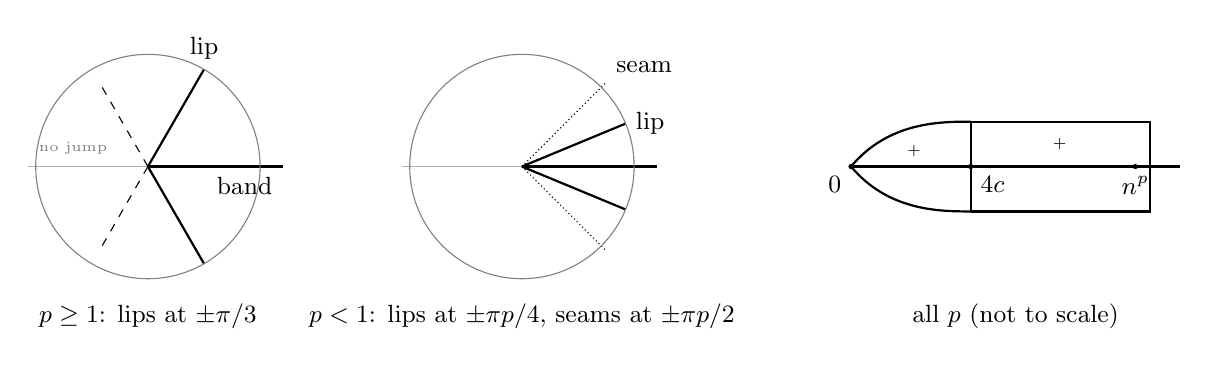
\begin{tikzpicture}[scale=0.95,>=Stealth]
  % panel 1: p >= 1
  \begin{scope}
    \draw[gray!60] (-1.6,0)--(0,0);
    \draw[thick] (0,0)--(1.8,0) node[below left]{\small band};
    \draw[thick] (0,0)--(60:1.5) node[above]{\small lip};
    \draw[thick] (0,0)--(-60:1.5);
    \draw[dashed] (0,0)--(120:1.3);
    \draw[dashed] (0,0)--(-120:1.3);
    \draw[gray] (0,0) circle (1.5);
    \node at (0,-2.0) {\small $p\ge1$: lips at $\pm\pi/3$};
    \node[gray] at (-1.0,0.25) {\tiny no jump};
  \end{scope}
  % panel 2: p < 1
  \begin{scope}[xshift=5cm]
    \draw[gray!60] (-1.6,0)--(0,0);
    \draw[thick] (0,0)--(1.8,0);
    \draw[thick] (0,0)--(22.5:1.5) node[right]{\small lip};
    \draw[thick] (0,0)--(-22.5:1.5);
    \draw[densely dotted] (0,0)--(45:1.6) node[above right]{\small seam};
    \draw[densely dotted] (0,0)--(-45:1.6);
    \draw[gray] (0,0) circle (1.5);
    \node at (0,-2.0) {\small $p<1$: lips at $\pm\pi p/4$, seams at $\pm\pi p/2$};
    \node[gray] at (-0.9,0.9) {\small $\Sout$};
    \node[gray] at (0.9,0.25) {\tiny $\Sin$};
  \end{scope}
  % panel 3: global
  \begin{scope}[xshift=9.4cm,yshift=0cm]
    \draw[thick] (0,0)--(4.4,0);
    \draw[thick] (0,0) .. controls (0.5,0.6) and (1.2,0.6) .. (1.6,0.6);
    \draw[thick] (0,0) .. controls (0.5,-0.6) and (1.2,-0.6) .. (1.6,-0.6);
    \draw[thick] (1.6,-0.6)--(1.6,0.6);
    \draw[thick] (1.6,0.6)--(4.0,0.6)--(4.0,-0.6)--(1.6,-0.6);
    \fill (0,0) circle (1pt) node[below left]{\small $0$};
    \fill (1.6,0) circle (1pt) node[below right]{\small $4c$};
    \fill (3.8,0) circle (1pt) node[below]{\small $n^p$};
    \node at (0.85,0.18) {\tiny $\Ob^+$};
    \node at (2.8,0.3) {\tiny $\Osat_+$};
    \node at (2.4,1.0) {\small $\Oinf$};
    \node at (2.2,-2.0) {\small all $p$ (not to scale)};
  \end{scope}
\end{tikzpicture}
\caption{The contour near the hard edge for $p\ge1$ and $p<1$ (Bessel rays dashed), and the whole contour. The
negative axis and, for $p<1$, the seams carry no jump of $V$ or $Q$. The seams are used only to construct the outer
scalar (\S\ref{sec:outer-plt1}).}
\label{fig:geometry}
\end{figure}

\subsection{The transformations}\label{sec:frame-transf}
We now remove the poles, normalise at infinity and open the lens. The pattern is that of \ref{tool:T1}(b); since we
work in a one-sided variable, we write every factor out. Put, in $\C_\pm$,
\begin{equation}\label{eq:kappa}
  \kappa_\pm:=\frac1{1-e^{\mp2i\theta}},\qquad\text{so that}\qquad \kappa_\pm-1=e^{\mp2i\theta}\kappa_\pm,
\end{equation}
and note $|e^{\mp2i\theta}|<1$ in $\C_\pm\cap\Zn$ by~\eqref{eq:imtheta}, so $\kappa_\pm$ is analytic there. Define,
on $\Zn\cap\C_\pm$,
\begin{equation}\label{eq:LA}
  L_\pm:=\begin{pmatrix}1&\mp We^{\mp2i\theta}\kappa_\pm\\0&1\end{pmatrix},\qquad
  A_\pm:=\begin{pmatrix}1&0\\\mp e^{2n\varphi}/W&1\end{pmatrix},\qquad
  A^\triangle_\pm:=\begin{pmatrix}1&0\\\mp1/(\kappa_\pm W)&1\end{pmatrix}.
\end{equation}

\emph{Step 1: removal of the poles.} Let
\begin{equation}\label{eq:R}
  R:=U\ \text{in }\Oinf,\qquad R:=UL_\pm\ \text{in }\Ob^\pm,\qquad R:=UA^\triangle_\pm\,\kappa_\pm^{\sigma_3}\ \text{in }\Osat_\pm .
\end{equation}
The restriction of $R$ to each of the four regions $\Ob^\pm$, $\Osat_\pm$ extends continuously to the real axis,
including the nodes. Indeed, near $X_k$ all factors are meromorphic, and $1-e^{\mp2i\theta}=\pm2i\theta'(X_k)
(z-X_k)(1+O(z-X_k))$ because $e^{2i\theta(X_k)}=1$. In $\Ob^\pm$ the entry $\mp We^{\mp2i\theta}\kappa_\pm$ then has the
simple pole $W(X_k)/(2i\theta'(X_k)(z-X_k))=w(X_k)/(z-X_k)$, and $R_{j2}=U_{j2}-U_{j1}w(X_k)/(z-X_k)+O(1)$ is regular
by Lemma~\ref{lem:interp}. In $\Osat_\pm$, $\kappa_\pm^{-1}$ vanishes simply at $X_k$, which removes the pole of the
second column; the first column is $\kappa_\pm(U_{j1}\mp U_{j2}/(\kappa_\pm W))$, and the bracket vanishes at $X_k$
since $U_{j2}/(\kappa_\pm W)\to\pm U_{j1}(X_k)$, so the first column is regular too.

\emph{Step 2: normalisation.} $T:=e^{-n\gamma_p\sigma_3}Re^{n\varphi\sigma_3}$.

\emph{Step 3: the lens.} $S:=TA_\pm$ in $\Ob^\pm$, and $S:=T$ elsewhere.

\emph{Step 4: the outer scalar.} Given a function $F$ with the properties (O1)--(O2) of~\S\ref{sec:frame-outer}
below and its lens version $\tilde F$, let
\begin{equation}\label{eq:V}
  V:=C_\infty\,S\,\tilde F^{\sigma_3}\ \text{in }\Ob\cup\Osat,\qquad V:=C_\infty\,S\,F^{\sigma_3}\ \text{in }\Oinf,
\end{equation}
with a constant diagonal matrix $C_\infty$ fixed in Lemma~\ref{lem:normalisation}.

Composing the four steps, and using $\kappa_\pm^{\sigma_3}\tilde F^{\sigma_3}=F^{\sigma_3}$ in $\Osat_\pm$
(definition~\eqref{eq:Ftilde} below),
\begin{equation}\label{eq:VM}
  V=C_\infty e^{-n\gamma_p\sigma_3}\,U\,M,\qquad
  M:=\begin{cases}e^{n\varphi\sigma_3}F^{\sigma_3}&\text{in }\Oinf,\\
  L_\pm e^{n\varphi\sigma_3}A_\pm\tilde F^{\sigma_3}&\text{in }\Ob^\pm,\\
  A^\triangle_\pm e^{n\varphi\sigma_3}F^{\sigma_3}&\text{in }\Osat_\pm.\end{cases}
\end{equation}
Since $U$ is analytic off the nodes, the jump of $V$ on any arc of $\Sigma$ away from the nodes is $M_-^{-1}M_+$.

The factor in $\Osat_\pm$ is the product of the factors $\Pi^{-\sigma_3}(\cdot)$ and $V^\triangle_\pm$ of \ref{tool:T1}(b),
moved into one step, except that in $\Osat_-$ we have changed it by the scalar $-1$. With the literal product a constant
jump $-I$ would appear on the saturated segment.

\subsection{Where the weight is evaluated}\label{sec:frame-where}
The following bookkeeping explains why the three strips $\vartheta_p$ of Table~\ref{tab:geometry} differ.

\begin{lemma}[Where the weight is evaluated]\label{lem:weightdomain}
The functions $w$, $W$, $r_n$ and $W_0$ (defined in~\eqref{eq:W0}) are evaluated in this paper only at points of
$\Zn$: in the closures of $\Ob$ and $\Osat$ (minus the point $0$), which contain the band, the saturated segment,
the lips, the vertical segments, $\Sigma^{\triangle\pm}$ and the top segment, and at the points of the lips and of the sectors $\{|\arg z|\le\frac54\thlip\}\cap U(0,\delta)$ used in
\S\ref{sec:hardedge} and Appendix~\ref{app:apriori}, and on the top segment. The region $\Oinf$ never uses the
weight: there $M=e^{n\varphi\sigma_3}F^{\sigma_3}$ contains neither $w$ nor $W$. Consequently, for every such point
$\xi(z)=\log t(z)$ lies in $\{\re\xi\ge-c_0,\ |\im\xi|\le\thw/p\}\subset S_{\vartheta_p}$.
\end{lemma}
% src: ROUTE2 §2 (H_an) note (REVIEW_Plan48 F4); ROUTE2_plt1 §1 Lemma S_w; ROUTE2_xframe1 §2 "Strip needed"

\begin{proof}
By~\eqref{eq:VM}, $w$ and $W$ enter $V$ only in $\Ob\cup\Osat$, whose closure minus $\{0\}$ lies in $\Zn$
(\S\ref{sec:frame-contour}); the top segment has $|z|\le n^p+\delta'+h_0<e^{pc_0}n^p$ and $|\arg z|<\thw$. The sectors
used near $0$ lie in $\Zn$ because $\frac54\thlip<\thw$. For $z\in\Zn$, $\re\xi=\log n-\frac1p\log|z|>-c_0$ and
$|\im\xi|=|\arg z|/p<\thw/p$.
\end{proof}

For $p>1$ every argument up to $\thw<\pi$ would be allowed, and the hypothesis is the full strip $\pi/p$. For $p<1$
the same bookkeeping keeps all evaluations in the inner sector $|\arg z|<\pi p/2$, so the strip $\pi/2$ suffices; the
strip $\pi/p$ would be wider than needed, and wider than the strip on which, for example,
$\Lambda(\xi)=\sqrt{\log(e^\xi+e)}$ is analytic. At $p=1$ the strip is $\pi/2$ for the same reason.

\begin{lemma}[Potter bounds in the sector]\label{lem:pottersector}
For every $\eta>0$ there is $C_\eta$ such that:
\begin{enumerate}
\item[(i)] $|\Lambda(\xi)|\le C_\eta+\eta\re\xi$ for $\xi\in S_{\vartheta_p}$, $\re\xi\ge0$, and $|\Lambda|\le C$ on
  $S_{\vartheta_p}\cap\{\re\xi\le0\}$. Hence $|\ell_1(t)|^{\pm1}\le C_\eta|t|^\eta$ for $|\arg t|\le\vartheta_p$,
  $|t|\ge1$.
\item[(ii)] $|r_n(z)|^{\pm1}\le C_\eta n^{2\eta}(1+|z|^{-\eta/p})$ for $z\in\Zn$.
\item[(iii)] For $R\ge1$, $z\in\Zn$ with $|z|\le R$ and $x\in(0,R]$,
  \begin{gather*}
    |\log r_n(z)-\log r_n(x)|\le\frac{\eps_\Lambda(T)}p\bigl(|\arg z|+|\log(x/|z|)|\bigr),\\
    |\log r_n(z)|\le\frac{\eps_\Lambda(T)}p\bigl(|\arg z|+|\log|z||\bigr),
  \end{gather*}
  with $T:=\log n-\frac1p\log R$. Here $\log r_n=\Lambda(\xi)-\Lambda(\log n)$.
\end{enumerate}
\end{lemma}
% src: ROUTE2 §2 "Consequences ... Potter in the sector"; ROUTE2 §3.3 (path); ROUTE2_plt1 §1

\begin{proof}
(i) For $\re\xi\ge T_0$, integrate $\Lambda'$ along the horizontal segment from $T_0+i\im\xi$ to $\xi$:
$|\Lambda(\xi)-\Lambda(T_0+i\im\xi)|\le\eps_\Lambda(T_0)\re\xi$. Choose $T_0$ with $\eps_\Lambda(T_0)\le\eta$; $\Lambda$ is
bounded on the compact set $S_{\vartheta_p}\cap\{0\le\re\xi\le T_0\}$ and, by hypothesis, on $\re\xi\le0$. Then
$|\ell_1(t)|^{\pm1}=e^{\pm\re\Lambda(\log t)}$.
(ii) $|r_n|^{\pm1}=|\ell_1(t)|^{\pm1}\ell_1(n)^{\mp1}$ with $|t|=n|z|^{-1/p}$; apply~(i) to both factors (for $|t|\le1$ use
the bound on $\re\xi\le0$).
(iii) Join $\xi(x)$ to $\xi(z)$ by the horizontal segment from $\log n-\frac1p\log x$ to $\log n-\frac1p\log|z|$
followed by the vertical segment to $\xi(z)$. Along this path $\re\xi\ge T$ and $|\im\xi|\le|\arg z|/p$, and its length
is $(|\log(x/|z|)|+|\arg z|)/p$. The second inequality is the case $x=1$, since $r_n(1)=1$.
\end{proof}

\subsection{The outer scalar and the jumps of $V$}\label{sec:frame-outer}
\S\ref{sec:outer} constructs, for each geometry, a function $F$ with the following five properties. The constants in
(O3) and (O4) do not depend on $n$; $\nu_p:=\min(1/p,\frac12)$, and $\eta_0\in(0,\delta]$ is fixed.
\begin{enumerate}
\item[(O1)] $F$ is analytic and zero-free in $\C\setminus[0,\infty)$ (in particular, it has no jump on $(-\infty,0)$),
  it has continuous boundary values on $(0,\infty)\setminus\{X_k\}$, and $F_+=F_-e^{2i\theta}$ on
  $(4c,\infty)\setminus\{X_k\}$.
\item[(O2)] The \emph{lens scalar}
  \begin{equation}\label{eq:Ftilde}
    \tilde F:=(1-e^{\mp2i\theta})F=F/\kappa_\pm\qquad\text{in }\C_\pm\cap\Zn
  \end{equation}
  extends to an analytic, zero-free function on $\Zn\setminus[4c,\infty)$, with $\tilde F_+=-\tilde F_-$ on
  $(4c,e^{pc_0}n^p)$. Thus $\tilde F^2$ is analytic and zero-free on $\Zn$, and so is the \emph{band factor}
  \begin{equation}\label{eq:Hn}
    H_n(z):=\frac1{(4c-z)\tilde F(z)^2}\qquad(z\in\Zn).
  \end{equation}
  We require $H_n>0$ on $(0,e^{pc_0}n^p)$ and that $H_n(0^+):=\lim_{z\to0,\,z\in\Zn}H_n(z)$ exists in $(0,\infty)$.
\item[(O3)] For $z\in\Zn$ with $|z|\le\eta_0$:
  $|\log H_n(z)-\log H_n(0^+)|\le C|z|^{\nu_p}$ and $|(\log H_n)'(z)|\le C|z|^{\nu_p-1}$.
\item[(O4)] For $z\in\Zn$ with $|z|\ge\eta_0$: $|\log H_n(z)-\log H_n(0^+)|\le C\bigl(1+\log(1+|z|)\bigr)^2$.
\item[(O5)] (For each fixed $n$.) $|F|^{\pm1}$ is bounded on $U(0,\delta)\setminus(\overline{\Ob}\cup[0,\infty))$, and
  $\tilde F^{\pm1}$ is bounded on $U(0,\delta)\cap\Ob$. There is $m_n$ with $|F(z)|^{\pm1}\le C_n|z|^{m_n}$ for
  $|z|\ge n^p+\delta'$, $z\notin\R$, and $F(iy)$ is bounded and bounded away from $0$ as $y\to\pm\infty$.
\end{enumerate}
The \emph{band weight} is
\begin{equation}\label{eq:W0}
  W_0:=\frac W{\tilde F^2}=C_n\,z^\alpha(4c-z)H_n(z)r_n(z)\quad\text{on }\Zn,\qquad C_n:=C_n'
\end{equation}
(Lemma~\ref{lem:bandweight}). On $(0,4c)$ it equals $C_n$ times a positive function.

\begin{lemma}[Jumps of $V$]\label{lem:jumpsV}
Assume (O1) and (O2). Then $V$ is analytic in $\C\setminus\Sigma$, has continuous boundary values on $\Sigma$ minus its
vertices (including at the nodes), and $V_+=V_-v_V$ with
\begin{enumerate}
\item[(a)] on the band $(0,4c)$: $v_V=\begin{pmatrix}0&W_0\\-1/W_0&0\end{pmatrix}$;
\item[(b)] on $\Sigma^\pm_{\mathrm{lip}}$ (oriented away from $0$), with $\epsilon_+=1$ and $\epsilon_-=0$:
  \[
    v_V=\begin{pmatrix}1&0\\e^{2n\varphi}/W_0&1\end{pmatrix}
    +\begin{pmatrix}\epsilon_\pm(\kappa_\pm-1)&W_0e^{-2n\tvphi}\\(\kappa_\pm-1)e^{2n\varphi}/W_0&\epsilon_\mp(\kappa_\pm-1)\end{pmatrix};
  \]
\item[(c)] on $\Sigma_v^\pm$ (oriented away from the real axis): $v_V=\begin{pmatrix}1&-W_0e^{-2n\tvphi}\\0&1\end{pmatrix}$;
\item[(d)] on the saturated segment $(4c,n^p+\delta')$: $v_V=\begin{pmatrix}1&0\\e^{2n\tvphi}/W_0&1\end{pmatrix}$;
\item[(e)] on $\Sigma^{\triangle\pm}$ (oriented from left to right): $v_V=\begin{pmatrix}1&0\\\kappa_\pm e^{2n\varphi}/W_0&1\end{pmatrix}$;
\item[(f)] on $\Sigma_{\mathrm{top}}\cap\C_\pm$ (oriented upwards): $v_V=\begin{pmatrix}1&0\\\mp\kappa_\pm e^{2n\varphi}/W_0&1\end{pmatrix}$;
\item[(g)] there is no jump on $(-\infty,0)$ or on $(n^p+\delta',\infty)$.
\end{enumerate}
\end{lemma}
% src: RH_px §3 "Facts about the jumps", §4.2, §4.3; RH_zeta_close §1.0; WLXZ (6.4) (T1); all recomputed here.

\begin{proof}
We use $M_-^{-1}M_+$ from~\eqref{eq:VM} and the identities
\begin{equation}\label{eq:identities}
  e^{\mp2i\theta}e^{-2n\varphi}=e^{-2n\tvphi},\qquad F=\kappa_\pm\tilde F,\qquad W/\tilde F^2=W_0\qquad\text{in }\C_\pm .
\end{equation}
For a diagonal matrix $D=\mathrm{diag}(d_1,d_2)$, conjugation $D^{-1}XD$ multiplies the $(1,2)$ entry by $d_2/d_1$ and the
$(2,1)$ entry by $d_1/d_2$.

(a) $L_-^{-1}L_+=\bigl(\begin{smallmatrix}1&W\\0&1\end{smallmatrix}\bigr)$: its $(1,2)$ entry is
$-W(e^{-2i\theta}\kappa_++e^{2i\theta}\kappa_-)=-W\bigl(\frac{e^{-2i\theta}}{1-e^{-2i\theta}}+\frac1{e^{-2i\theta}-1}\bigr)=W$. Conjugating by $e^{n\varphi_\pm\sigma_3}$ and using $\varphi_-=-\varphi_+$
(Lemma~\ref{lem:gfunction}(i)) gives $\bigl(\begin{smallmatrix}e^{2n\varphi_+}&W\\0&e^{2n\varphi_-}\end{smallmatrix}\bigr)$, and
\[
  A_-^{-1}\begin{pmatrix}e^{2n\varphi_+}&W\\0&e^{2n\varphi_-}\end{pmatrix}A_+=\begin{pmatrix}0&W\\-1/W&0\end{pmatrix}.
\]
Since $\tilde F$ has no jump on the band (O2), the final conjugation gives~(a) by~\eqref{eq:identities}.

(b) Upper lip: the $+$ side is $\Oinf$, so $v_V=M_{\Ob}^{-1}M_{\Oinf}=\tilde F^{-\sigma_3}A_+^{-1}\bigl(e^{-n\varphi\sigma_3}
L_+^{-1}e^{n\varphi\sigma_3}\bigr)F^{\sigma_3}$. The bracket is $\bigl(\begin{smallmatrix}1&W\kappa_+e^{-2n\tvphi}\\0&1
\end{smallmatrix}\bigr)$, and
\[
  A_+^{-1}\begin{pmatrix}1&W\kappa_+e^{-2n\tvphi}\\0&1\end{pmatrix}=
  \begin{pmatrix}1&W\kappa_+e^{-2n\tvphi}\\e^{2n\varphi}/W&\kappa_+\end{pmatrix},
\]
because $1+\kappa_+e^{2n\varphi}e^{-2n\tvphi}=1+\kappa_+e^{-2i\theta}=\kappa_+$. Conjugating with $\tilde F^{-\sigma_3}(\cdot)F^{\sigma_3}$,
$F=\kappa_+\tilde F$, gives $\bigl(\begin{smallmatrix}\kappa_+&W_0e^{-2n\tvphi}\\\kappa_+e^{2n\varphi}/W_0&1\end{smallmatrix}\bigr)$,
which is~(b). The lower lip (where the $+$ side is the lens) is the mirror computation and gives
$\bigl(\begin{smallmatrix}1&W_0e^{-2n\tvphi}\\\kappa_-e^{2n\varphi}/W_0&\kappa_-\end{smallmatrix}\bigr)$.

(c) Upper segment, $+$ side $=\Ob^+$: $v_V=M_{\Osat}^{-1}M_{\Ob}=F^{-\sigma_3}e^{-n\varphi\sigma_3}(A^\triangle_+)^{-1}L_+
e^{n\varphi\sigma_3}A_+\tilde F^{\sigma_3}$. One checks $(A^\triangle_+)^{-1}L_+=\bigl(\begin{smallmatrix}1&-We^{-2i\theta}
\kappa_+\\1/(\kappa_+W)&1-e^{-2i\theta}\end{smallmatrix}\bigr)$, and after the conjugation by $e^{n\varphi\sigma_3}$ and right
multiplication by $A_+$ the $(2,1)$ entry vanishes and the diagonal becomes $(\kappa_+,\kappa_+^{-1})$; the final
conjugation with $F=\kappa_+\tilde F$ removes the diagonal and gives~(c). The lower segment is the mirror image.

(d) On $(4c,n^p+\delta')$ both sides lie in $\Osat$. Since $\kappa_\pm^{-1}=1-e^{\mp2i\theta}$,
$(A^\triangle_-)^{-1}A^\triangle_+=\bigl(\begin{smallmatrix}1&0\\-(\kappa_+^{-1}+\kappa_-^{-1})/W&1\end{smallmatrix}\bigr)$, and
$\kappa_+^{-1}+\kappa_-^{-1}=2-2\cos2\theta=\kappa_+^{-1}\kappa_-^{-1}$. Conjugating by $e^{n\varphi\sigma_3}F^{\sigma_3}$ with
boundary values, the diagonal is $(e^{n(\varphi_+-\varphi_-)}F_+/F_-)^{\sigma_3}=(e^{-2i\theta}e^{2i\theta})^{\sigma_3}=I$
by Lemma~\ref{lem:gfunction}(i) and (O1), and the $(2,1)$ entry is
$-e^{n(\varphi_++\varphi_-)}F_+F_-/(\kappa_+\kappa_-W)=-e^{2n\tvphi}\tilde F_+\tilde F_-/W$. By (O2),
$-\tilde F_+\tilde F_-=\tilde F^2$, which gives~(d).

(e), (f) Here $v_V=(F^{-\sigma_3}e^{-n\varphi\sigma_3})(A^\triangle_\pm)^{\pm1}(e^{n\varphi\sigma_3}F^{\sigma_3})$ with the
exponent fixed by the orientation, and the $(2,1)$ entry $\mp1/(\kappa_\pm W)$ of $A^\triangle_\pm$ becomes
$\mp F^2e^{2n\varphi}/(\kappa_\pm W)=\mp\kappa_\pm e^{2n\varphi}/W_0$.

(g) On $(-\infty,0)$: $U$ has no jump, $e^{n\varphi}$ jumps by $e^{-2\pi in}=1$ (Lemma~\ref{lem:gfunction}(i)) and $F$ has no
jump (O1). On $(n^p+\delta',\infty)$ there are no nodes, and $M_-^{-1}M_+=(e^{n(\varphi_+-\varphi_-)}F_+/F_-)^{\sigma_3}=I$ as
in~(d).

Continuity at the nodes: in~(a) and~(d) all entries are analytic across the real axis; together with Step~1 this shows
that $V$ has continuous boundary values there.
\end{proof}

\begin{table}[ht]
\centering\small
\renewcommand{\arraystretch}{1.25}
\begin{tabular}{@{}p{3.4cm}p{3.2cm}p{3.2cm}p{3.6cm}@{}}
\toprule
& $p>1$ & $p=1$ & $0<p<1$\tabularnewline
\midrule
\raggedright $\arg t$ on $\C\setminus(-\infty,0]$ & \raggedright $(-\pi/p,\pi/p)\subset(-\pi,\pi)$ & \raggedright $(-\pi,\pi)$, open & \raggedright wider than $(-\pi,\pi)$; poles of $\Gamma(t)$ on $\arg z=\pm\pi p$\tabularnewline
\raggedright where $\tilde D=e^{-j(t)}$ is used & \raggedright slit plane & \raggedright $|\arg z|\le\thw=7\pi/16$ & \raggedright inner sector $\Sin=\{|\arg z|<\pi p/2\}$\tabularnewline
\raggedright outer scalar $F$ & \raggedright $DBK$, Binet-cut scalar $B$ (Lemma~\ref{lem:binetcut}) & \raggedright $DK$, $D=e^{j(-n/z)}$, no cut (Lemma~\ref{lem:reflection}) & \raggedright $DB_{\mathrm{in}}Ke^{\chi}$ in $\Sin$, $B_{\mathrm{out}}Ke^{\chi}$ in $\Sout$ (Lemma~\ref{lem:seam})\tabularnewline
\raggedright $|\log\frac{H_n(z)}{H_n(0^+)}|$ near $0$ & \raggedright $\le C|z|^{1/p}$ & \raggedright $\le C|z|$ & \raggedright $\le C|z|(1+\log\frac1{|z|})$\tabularnewline
\raggedright $g(z)-\log z$ at $\infty$ & \raggedright $O(|z|^{-1/p})$ & \raggedright $O(|z|^{-1}\log|z|)$ & \raggedright $O(|z|^{-1})$\tabularnewline
\raggedright lip angle $\thlip$; Bessel rays & \raggedright $\pi/3$; $\pm2\pi/3$ & \raggedright $\pi/3$; $\pm2\pi/3$ & \raggedright $\pi p/4$; $\pm(\pi-\pi p/4)$\tabularnewline
\raggedright angle $\thw$ (weight evaluated) & \raggedright $7\pi/16$ & \raggedright $7\pi/16$ & \raggedright $3\pi p/8$\tabularnewline
\raggedright super-small entries $|e^{\mp2i\theta}|$ on the lips & \raggedright $e^{-2\pi n\sin(\frac{\pi}{3p})|z|^{-1/p}}$ & \raggedright $e^{-\sqrt3\pi n/|z|}$ & \raggedright $e^{-\sqrt2\pi n|z|^{-1/p}}$\tabularnewline
\raggedright strip $\vartheta_p$ for $\ell_1$ & \raggedright $\pi/p$ & \raggedright $\pi/2$ & \raggedright $\pi/2$\tabularnewline
\raggedright $\nu_p$ (in $\eps'_n=n^{-2\nu_p}\log n+\eps_\Lambda(T_n)$) & \raggedright $\min(1/p,\frac12)$ & \raggedright $\frac12$ & \raggedright $\frac12$\tabularnewline
\raggedright classical quotient parametrix at $0$ & \raggedright works for pure powers (not used) & \raggedright fails (Remark~\ref{rem:quotient-p1}) & \raggedright works with a seam glue (not used)\tabularnewline
\bottomrule
\end{tabular}
\caption{The ingredients of the Riemann--Hilbert analysis that depend on the geometry. Everything else in
\S\S\ref{sec:frame}--\ref{sec:extraction} is the same for all $p>0$. The super-small entries are evaluated on the rays
$\arg z=\pm\thlip$; $\eps'_n$ is the lip-mismatch size of \S\ref{sec:hardedge}.}
\label{tab:geometry}
\end{table}

% ===================================================================================
% Section 6 (chunk C): the outer scalar in the three geometries; the Frame Proposition.
% Labels defined here: sec:outer, sec:outer-pgt1, sec:outer-p1, sec:outer-plt1, sec:outer-common,
%   lem:binetcut, lem:reflection, rem:quotient-p1, lem:seam, lem:corner, lem:szego, lem:normalisation,
%   lem:supersmall, prop:frame, eq:*.
% Uses: sec_5.tex (lem:interp, lem:bandweight, lem:gfunction, lem:signs, lem:weightdomain, lem:pottersector,
%   lem:jumpsV, (O1)-(O5)), tool:T1, tool:T2, tool:T3, tool:T4, lem:invariance (Sect. 8), lem:B-block (App. B).
% ===================================================================================
\providecommand{\eps}{\varepsilon}
\providecommand{\Log}{\operatorname{Log}}
\providecommand{\re}{\operatorname{Re}}
\providecommand{\im}{\operatorname{Im}}
\providecommand{\thlip}{\vartheta_{\mathrm{lip}}}
\providecommand{\thseam}{\vartheta_{\mathrm{seam}}}
\providecommand{\thw}{\vartheta_{\mathrm{w}}}
\providecommand{\Ob}{\Omega_{\mathrm{b}}}
\providecommand{\Osat}{\Omega^{\triangle}}
\providecommand{\Oinf}{\Omega_{\infty}}
\providecommand{\Sin}{S_{\mathrm{in}}}
\providecommand{\Sout}{S_{\mathrm{out}}}
\providecommand{\Zn}{\mathcal{Z}_n}
\providecommand{\tvphi}{\tilde\varphi}
\providecommand{\Fi}[1]{\textup{(F#1)}}
\providecommand{\Cauchy}{\mathcal{C}}
\providecommand{\dC}{\partial\mathcal{C}}

\section{The outer scalar in three geometries}\label{sec:outer}

The transformations of \S\ref{sec:frame} reduce everything away from the hard edge to one scalar problem: find an
outer scalar $F$ with the properties (O1)--(O5) of \S\ref{sec:frame-outer}. The natural candidate comes from
Stirling's formula. The node masses carry the factor $1/\Gamma(t)$ through $\Pi=\sin\theta/\theta'$, and
\[
  \tilde D(z):=e^{-j(t(z))},\qquad j(t):=\operatorname{Ln}\Gamma(t)-\bigl(t-\tfrac12\bigr)\ln t+t-\tfrac12\ln(2\pi),
\]
removes this growth. Here $j$ is Binet's function, $\operatorname{Ln}\Gamma$ is the branch analytic on
$\C\setminus(-\infty,0]$ and real on $(0,\infty)$, and $\ln t$ is principal; so
$\tilde D=\sqrt{2\pi}\,t^{t-1/2}e^{-t}/\Gamma(t)$, and this sign convention is used throughout. Then
\begin{equation}\label{eq:D}
  D:=\kappa_\pm\tilde D=\frac{\tilde D}{1-e^{\mp2i\theta}}\quad\text{in }\C_\pm
\end{equation}
satisfies $D_+/D_-=(1-e^{2i\theta})/(1-e^{-2i\theta})=-e^{2i\theta}$ on $(0,\infty)$ off the nodes, and
$K(z):=(4c-z)^{-1/2}$ (principal branch, cut $[4c,\infty)$) supplies the missing factor $-1$, so that $DK$ has the
jump required in (O1).

The difficulty is the cut of $t(z)$ on $(-\infty,0)$. How it is handled depends on how far the sector of $t$ reaches.
For $p>1$, $|\arg t|<\pi/p<\pi$ on the slit plane: $\Gamma(t)$ has no poles there, and $DK$ has a jump on
$(-\infty,0)$ which is removed exactly by a Cauchy integral, the Binet-cut scalar $B$ (\S\ref{sec:outer-pgt1}). At
$p=1$ the sector is exactly $|\arg t|<\pi$, and the reflection formula shows that $D$ has no jump at all on
$(-\infty,0)$ (\S\ref{sec:outer-p1}). For $p<1$ the sector of $t$ is wider than $(-\pi,\pi)$ and the poles of $\Gamma$
enter; we then use $D$ only in the inner sector $|\arg z|<\pi p/2$ and glue it to an elementary function outside
along two seams, with an exact scalar $\chi$ (\S\ref{sec:outer-plt1}). \S\ref{sec:outer-common} is common to all
geometries: Szeg\H{o} functions, the normalisation at infinity, the super-small entries, the two parametrices away from
$0$, and the Frame Proposition, which is the only input of \S\S\ref{sec:hardedge}--\ref{sec:extraction} from this
section.

Two facts about $j$ are used in all three geometries. By \ref{tool:T4} (DLMF 5.11.1 with the remainder bound of
\S5.11(ii), first term $1/(12t)$), for every $\vartheta<\pi$,
\begin{equation}\label{eq:binet-bound}
  |j(t)|\le\frac{\sec^2(\vartheta/2)}{12|t|},\qquad |j'(t)|\le\frac{C_\vartheta}{|t|^2}\qquad(|\arg t|\le\vartheta,\ |t|\ge1),
\end{equation}
the second by Cauchy's estimate on a disc of radius $c_\vartheta|t|$ in a slightly larger sector. And for $|t|\le1$,
$\re t\ge0$, $t\ne0$, DLMF 5.5.1 gives $\operatorname{Ln}\Gamma(t)=\operatorname{Ln}\Gamma(1+t)-\ln t$, hence
\begin{equation}\label{eq:binet-small}
  j(t)=-\tfrac12\ln t-\tfrac12\ln(2\pi)+O(|t|\log(2/|t|))\qquad(t\to0,\ \re t\ge0).
\end{equation}

\subsection{The case $p>1$: the Binet-cut scalar}\label{sec:outer-pgt1}

\begin{lemma}[Binet-cut scalar]\label{lem:binetcut}
Let $p>1$.
\begin{enumerate}
\item[(i)] $\tilde D$ is analytic and zero-free on $\C\setminus(-\infty,0]$, and $D$ is analytic and zero-free in
  $\C_\pm$, with continuous boundary values on $\R\setminus(\{X_k\}\cup\{0\})$. On $(-\infty,0)$, $D_-=\overline{D_+}$.
\item[(ii)] Let $\hat\ell(y):=2\im\bigl(-j(t_+(y))-\Log(1-e^{-2i\theta_+(y)})\bigr)$ for $y<0$, where $t_+,\theta_+$
  are boundary values from $\C_+$. Then $D_+/D_-=e^{i\hat\ell}$ on $(-\infty,0)$; $\hat\ell$ is real-analytic,
  $|\hat\ell(y)|\le C\min(1,|y|^{1/p})$ with $C$ independent of $n$, $|\hat\ell'(y)|\le C_n|y|^{1/p-1}$ for $-1\le y<0$,
  $\hat\ell'$ is bounded on $(-\infty,-\frac12]$, and $\hat\ell(y)\to\pi/p-\pi$ as $y\to-\infty$, with
  $\int_{-\infty}^{-1}|\hat\ell(y)-\pi/p+\pi|\,|y|^{-1}\diff y<\infty$.
\item[(iii)] The function
  \begin{equation}\label{eq:B}
    B(z):=\exp\Bigl(-\frac1{2\pi}\int_{-\infty}^0\hat\ell(y)\Bigl[\frac1{y-z}-\frac1{y-1}\Bigr]\diff y\Bigr)
  \end{equation}
  is analytic and zero-free on $\C\setminus(-\infty,0]$, positive on $(0,\infty)$, has continuous boundary values on
  $(-\infty,0)$ with $B_+=B_-e^{-i\hat\ell}$, and $DB$ extends analytically across $(-\infty,0)$. For $z\in\Zn$, with
  $C$ independent of $n$,
  \begin{equation}\label{eq:B-bounds}
  \begin{gathered}
    |\log B(z)-\log B(0)|\le C|z|^{1/p},\quad |(\log B)'(z)|\le C|z|^{1/p-1}\quad(|z|\le1),\\
    |\log B(z)|\le C(1+\log(1+|z|)).
  \end{gathered}
  \end{equation}
\item[(iv)] $F:=DBK$ satisfies (O1)--(O5), with $\tilde F=\tilde DBK$ and $H_n=(\tilde DB)^{-2}$.
\end{enumerate}
\end{lemma}
% src: RH_px Lemmas 1.1, 3.1, 3.2(i)-(iv), 3.3, 3.4 ("Consequence"); review REVIEW_RHpx (F4(b), exponent 1/2-1/(2p)).
% Lemma 3.2(v) of RH_px is not needed (OUTLINE §5, §6.1).

\begin{proof}
(i) On the slit plane $|\arg t|<\pi/p<\pi$, so $\Gamma(t)$ has neither zeros nor poles and $\tilde D$ is analytic and
zero-free. By~\eqref{eq:imtheta}, $|e^{\mp2i\theta}|<1$ in $\C_\pm$ (here $\pi p>\pi$), so $D$ is analytic and
zero-free in $\C_\pm$. On $(-\infty,0)$, $t_-=\overline{t_+}$ and $\Gamma$, $j$ are real on the real axis, so
$D_-=\overline{D_+}$.

(ii) Since $|e^{-2i\theta_+}|<1$ on $(-\infty,0)$, $\log D_+:=-j(t_+)-\Log(1-e^{-2i\theta_+})$ is a continuous
logarithm, real-analytic in $y$, and $D_+/D_-=e^{2i\im\log D_+}=e^{i\hat\ell}$. With $|t_+|=n|y|^{-1/p}$ and
$\arg t_+=-\pi/p$: for $|t_+|\ge1$, \eqref{eq:binet-bound} and
$|\Log(1-e^{-2i\theta_+})|\le2\exp(-2\pi\sin(\pi/p)|t_+|)$ give $|\hat\ell|\le C/|t_+|=C|y|^{1/p}/n$. For $|t_+|\le1$ the
expansion~\eqref{eq:binet-small} and $\Log(1-e^{-2\pi it})=\log(2\pi|t|)+i(\frac\pi2+\arg t)+O(t)$ (note
$\frac\pi2+\arg t_+\in(-\frac\pi2,\frac\pi2)$) show that $\hat\ell$ is bounded and
\[
  \hat\ell(y)=2\bigl(\tfrac12\arg t_+-\tfrac\pi2-\arg t_+\bigr)+O(|t_+|\log(2/|t_+|))=\frac\pi p-\pi+O\bigl(n|y|^{-1/p}\log|y|\bigr).
\]
This gives the bounds on $\hat\ell$ and the integrability. For the derivative, $\diff t_+/\diff y=-t_+/(py)$, and
$\frac{\diff}{\diff t}\bigl(j(t)+\Log(1-e^{-2\pi it})\bigr)$ is $O(|t|^{-2})$ for $|t|\ge1$ and $O(|t|^{-1})$ for
$|t|\le1$; multiplied by $|t|/|y|$ this gives $|\hat\ell'(y)|\le C|y|^{1/p-1}/n$ for $|y|\le n^p$ and
$|\hat\ell'(y)|\le C/|y|$ otherwise.

(iii) The integral converges absolutely, since $\hat\ell$ is bounded and the bracket is $(z-1)/((y-z)(y-1))$. By the
Sokhotski--Plemelj formula (the density is real-analytic on $(-\infty,0)$), $\log B$ has continuous boundary values
and $(\log B)_+-(\log B)_-=-i\hat\ell$. So $(DB)_+=(DB)_-$ on $(-\infty,0)$, and $DB$, being continuous across, is
analytic there by Morera's theorem. $B$ is positive on $(0,\infty)$ because the integrand is real there.

For~\eqref{eq:B-bounds}, let $z\in\Zn$. Then $|y-z|^2=y^2+|z|^2+2|y||z|\cos(\arg z)\ge\frac12(|y|+|z|)^2$ for $y<0$, since $|\arg z|<\thw<\pi/2$.
We have $\log B(z)-\log B(0)=-\frac z{2\pi}\int_{-\infty}^0\frac{\hat\ell(y)\diff y}{y(y-z)}$, so by~(ii), for $|z|\le1$,
\[
  |\log B(z)-\log B(0)|\le C|z|\int_0^\infty\frac{\min(1,u^{1/p})}{u(u+|z|)}\diff u\le
  C|z|\Bigl(\int_0^1\frac{u^{1/p-1}\diff u}{u+|z|}+1\Bigr)\le C|z|^{1/p},
\]
because $1/p-1\in(-1,0)$. The same splitting applied to $(\log B)'(z)=-\frac1{2\pi}\int\hat\ell(y)(y-z)^{-2}\diff y$
gives $C|z|^{1/p-1}$, and applied to the original integral gives $C(1+\log(1+|z|))$.

(iv) \emph{(O1).} $F$ is analytic and zero-free off $[0,\infty)$ by~(i), (iii) and the choice of $K$. On
$(4c,\infty)$ off the nodes, $F_+/F_-=(D_+/D_-)(K_+/K_-)=(-e^{2i\theta})(-1)$, since $B$ is analytic there.

\emph{(O2).} $\tilde F=F/\kappa_\pm=\tilde DBK$ is analytic and zero-free on $\C\setminus\bigl((-\infty,0]\cup[4c,\infty)\bigr)$,
and $\tilde F_+=-\tilde F_-$ on $(4c,\infty)$ because of $K$. Thus $H_n=1/((4c-z)\tilde F^2)=(\tilde DB)^{-2}$, which is
positive on $(0,\infty)$, and $H_n(0^+)=B(0)^{-2}$ because $\tilde D(z)\to1$ as $z\to0$ in $\Zn$ by~\eqref{eq:binet-bound}.

\emph{(O3), (O4).} $\log H_n-\log H_n(0^+)=2j(t)-2(\log B-\log B(0))$. For $z\in\Zn$, $|z|\le1$, we have $|t|\ge n$ and
$|\arg t|\le\thw/p$, so $|j(t)|\le C|z|^{1/p}/n$ and $|\frac{\diff}{\diff z}j(t)|=|j'(t)||t|/(p|z|)\le C|z|^{1/p-1}/n$.
Together with~\eqref{eq:B-bounds} and $\nu_p\le1/p$, this is (O3). For $|z|\ge1$ in $\Zn$ we have $|t|\ge e^{-c_0}$, so
$j(t)$ is bounded (by~\eqref{eq:binet-bound} for $|t|\ge1$ and by continuity on the compact set
$\{e^{-c_0}\le|t|\le1,\ |\arg t|\le\thw/p\}$), and~\eqref{eq:B-bounds} gives (O4).

\emph{(O5).} Fix $n$. Near $0$ and outside the lens, $|\arg z|\ge\frac34\thlip$, so $\kappa_\pm\to1$ by~\eqref{eq:imtheta}
and $\tilde D\to1$; $K$ is bounded; and $\log B$ is bounded on $U(0,\delta)\setminus(-\delta,0]$ uniformly up to the cut.
For the last point split $\int\hat\ell(y)/(y-z)\diff y$ into the window $|y-\re z|\le|\re z|/2$ and the rest. On the
window write $\hat\ell(y)=\hat\ell(\re z)+O(|y-\re z|\,|\re z|^{1/p-1})$ by~(ii); the constant part integrates to
$\hat\ell(\re z)\Log(\cdot)$ with a bounded logarithm (the endpoints of the window are at comparable distances from $z$),
and the rest is bounded; outside the window $|y-z|\ge c(|y|+|z|)$ and $|\hat\ell(y)|\le C|y|^{1/p}$ give a bounded
contribution. In the lens, $\tilde F=\tilde DBK$ is bounded above and below by the same facts.

Near $\infty$, the same window argument on $(-\infty,-\frac12]$, where $\hat\ell'$ is bounded, gives
$|\log B(z)|\le C_n(1+\log|z|)$ for $|z|\ge2$ off the cut. For $|z|\ge n^p+\delta'$ we have $|t|<1$, and $t$ stays away from
$1$, so $D$ is bounded above and below by a power of $|z|$; hence $|F|^{\pm1}\le C_n|z|^{m_n}$. Finally, along $z=iy$,
$y\to\pm\infty$: by~\eqref{eq:binet-small}, $|D(iy)|=|t|^{-1/2}(2\pi)^{-1/2}(1+o(1))\asymp|y|^{1/(2p)}$; $|K(iy)|\asymp|y|^{-1/2}$;
and splitting $\hat\ell=(\pi/p-\pi)\mathbf 1_{(-\infty,-1)}+e$, the first part contributes
$-\frac{\pi/p-\pi}{2\pi}\Log\frac{z+1}{2}$ to $\log B$ (an explicit integral), while the second contributes a quantity with a
finite limit, by dominated convergence and the integrability in~(ii). So $|B(iy)|\asymp|y|^{\frac12-\frac1{2p}}$, and
$|F(iy)|\asymp1$.
\end{proof}

\subsection{The case $p=1$: reflection}\label{sec:outer-p1}
At $p=1$ the cut of $D$ disappears. This makes $p=1$ a simplification of the case $p>1$, not a special case.

\begin{lemma}[Reflection]\label{lem:reflection}
Let $p=1$, so $t=n/z$. For $z\in\C_\pm$,
\begin{equation}\label{eq:reflection}
  D(z)=\frac{e^{-j(t)}}{1-e^{\mp2\pi it}}=e^{j(-n/z)} .
\end{equation}
Hence $D$ extends analytically to $\C\setminus[0,\infty)$, and it is real and positive on $(-\infty,0)$. The function
$F:=DK$ satisfies (O1)--(O5), with $\tilde F=\tilde DK$ and $H_n=e^{2j(n/z)}$.
\end{lemma}
% src: ROUTE2_xframe1 §1 Lemma X1 (REVIEWED; DLMF 5.5.1, 5.5.3, 5.11.1); REVIEW_Plan54 §2, F1, F8.

\begin{proof}
Let $z\in\C_+$, so $\arg t\in(-\pi,0)$ and $t\notin\R$. By DLMF 5.5.3 (\ref{tool:T4}), $1/\Gamma(t)=\Gamma(1-t)\sin(\pi
t)/\pi$, and $\sin(\pi t)/(1-e^{-2\pi it})=e^{i\pi t}/(2i)$. Hence
$D=\sqrt{2\pi}\,t^{t-1/2}e^{-t}\Gamma(1-t)e^{i\pi t}/(2\pi i)$. Put $u:=-t=-n/z$; then $\arg u=\arg t+\pi\in(0,\pi)$, so
$\ln u=\ln t+i\pi$ for the principal branches, and
$t^{t-1/2}e^{i\pi t}=\exp((t-\frac12)(\ln u-i\pi)+i\pi t)=e^{i\pi/2}u^{-u-1/2}$. So $D=u^{-u-1/2}e^u\Gamma(1+u)/\sqrt{2\pi}$,
and DLMF 5.5.1 ($\Gamma(1+u)=u\Gamma(u)$) together with the definition of $j$ gives $D=e^{j(u)}$. For $z\in\C_-$ the same
computation with $\sin(\pi t)/(1-e^{2\pi it})=-e^{-i\pi t}/(2i)$ and $\ln u=\ln t-i\pi$ gives the same result. Since $j$ is
analytic on $\C\setminus(-\infty,0]$ and $u\in(-\infty,0]$ exactly when $z\in(0,\infty)$, $e^{j(-n/z)}$ is analytic on
$\C\setminus[0,\infty)$; on $(-\infty,0)$, $u>0$ and $j(u)$ is real.

\emph{(O1).} $F=DK$ is analytic and zero-free off $[0,\infty)$, and $F_+/F_-=(-e^{2i\theta})(-1)$ on $(4c,\infty)$ off the
nodes, as for $p>1$.

\emph{(O2).} $\tilde F=F/\kappa_\pm=\tilde DK$ with $\tilde D=e^{-j(t)}$ analytic and zero-free on $\C\setminus(-\infty,0]$.
So $H_n=\tilde D^{-2}=e^{2j(n/z)}>0$ on $(0,\infty)$, and $H_n(0^+)=1$.

\emph{(O3), (O4).} On $\Zn$, $|\arg t|=|\arg z|\le\thw=7\pi/16$. For $|z|\le1$, $|t|\ge n$ and~\eqref{eq:binet-bound}
gives $|\log H_n|=2|j(t)|\le C|z|/n$ and $|(\log H_n)'|\le C/n$; since $\nu_1=\frac12$, this is (O3). For $|z|\ge1$,
$|t|\ge e^{-c_0}$ and $j(t)$ is bounded, which is (O4).

\emph{(O5).} Fix $n$. Near $0$ outside the lens, $u=-n/z$ has $|u|\to\infty$ and $|\arg u|=\pi-|\arg z|\le\pi-\frac34\thlip$,
so $j(u)\to0$ by~\eqref{eq:binet-bound} and $D\to1$; $K$ is bounded. In the lens $\tilde F=\tilde DK$ with $\tilde D\to1$.
For $|z|\ge n+\delta'$ we have $|u|\le n/(n+\delta')<1$ and $|1+u|\ge\delta'/(2n)$, and
$D=u^{-u-1/2}e^u\Gamma(1+u)/\sqrt{2\pi}$ is bounded above and below by $C_n|z|^{\pm1}$. Along $z=iy$, $D(iy)=(-iy/n)^{1/2}
(2\pi)^{-1/2}(1+o(1))$ by~\eqref{eq:binet-small}, and $K(iy)=(-iy)^{-1/2}(1+o(1))$, so $F(iy)\to(2\pi n)^{-1/2}$.
\end{proof}

\begin{remark}[The classical hard-edge parametrix at $p=1$]\label{rem:quotient-p1}
For pure powers and $p\ne1$, one can also build the hard-edge parametrix in the classical way, as in \ref{tool:T2}, from
a square root $\tilde W$ of the band weight continued to a full neighbourhood of $0$; for $p>1$ its jump on
$(-\delta,0)$ is super-exponentially close to $I$, because $|e^{\mp2i\theta}|=\exp(-2\pi n\sin(\pi/p)|x|^{-1/p})$ there. At
$p=1$ this particular construction fails, already for $\ell_1\equiv1$. On $(-\delta,0)$, $\theta=\pi n/x$ is real, and
the continuations of the lens scalar from the two half-planes differ by
$\tilde F_+/\tilde F_-=(1-e^{-2i\theta})/(1-e^{2i\theta})=-e^{-2i\theta}$ (because $F$ has no jump there): a unimodular factor
that is not close to $1$. Moreover the continuation of $H_n=e^{2j(n/z)}$ across $(-\delta,0)$ has double poles at the
points $z=-n/m$, $m\in\N$, which accumulate at $0$. Our route never uses this construction: the comparison parametrix
of \S\ref{sec:hardedge} uses only the Szeg\H{o} function $D_W$ of the band values, which has no jump on
$(-\delta,0)$, and nothing is continued across $(-\delta,0)$. The obstruction concerns this classical construction
as written, not every quotient construction.
\end{remark}
% src: ROUTE2_xframe1 §1 Lemma X2 + Scope; REVIEW_Plan54 F2 (scope wording).

\subsection{The case $0<p<1$: seams}\label{sec:outer-plt1}
For $p<1$ the poles $t=-1,-2,\dots$ of $\Gamma$ lie on the rays $\arg z=\pm\pi p$, inside the slit plane, and $D$ has
no useful continuation to the negative axis. We use $D$ only in the inner sector, where $|\arg t|<\pi/2$, and an
elementary function outside; a Cauchy integral $\chi$ over the two separating rays glues them together exactly. Put
\begin{gather*}
  \thseam:=\tfrac{\pi p}2,\qquad \Sin:=\{z\ne0:\ |\arg z|<\thseam\},\qquad \Sout:=\C\setminus(\overline{\Sin}\cup\{0\}),\\
  \Gamma_\pm:=\{re^{\pm i\thseam}:\ r>0\},
\end{gather*}
both seams oriented away from $0$, and
\[
  \varpi:=\tfrac12-\tfrac1{2p}<0,\qquad B_{\mathrm{in}}(z):=(1+z)^{\varpi},\qquad B_{\mathrm{out}}(z):=\Bigl(1-\frac z{2\pi n}\Bigr)^{1/2},
\]
with principal powers; the cut $(-\infty,-1]$ of $B_{\mathrm{in}}$ lies in $\Sout$, and the cut $[2\pi n,\infty)$ of
$B_{\mathrm{out}}$ lies in $\Sin$. The lens, the saturated regions and the top segment lie in $\Zn\subset\Sin$, since
$\thw=3\pi p/8<\thseam$.

\begin{lemma}[Seam scalar]\label{lem:seam}
Let $0<p<1$.
\begin{enumerate}
\item[(i)] On $\Sin$, $|\arg t|<\pi/2$; $\tilde D=e^{-j(t)}$ is analytic and zero-free there, and $D=\kappa_\pm\tilde D$ is
  analytic and zero-free in $\Sin\cap\C_\pm$.
\item[(ii)] On $\Gamma_\pm$ put, with principal logarithms,
  \begin{equation}\label{eq:Lpm}
    L_\pm(\zeta):=-j(t(\zeta))-\Log\bigl(1-e^{\mp2\pi it(\zeta)}\bigr)+\varpi\Log(1+\zeta)-\tfrac12\Log\Bigl(1-\frac\zeta{2\pi n}\Bigr).
  \end{equation}
  Then $L_\pm$ is real-analytic on the open ray, $e^{L_\pm}=DB_{\mathrm{in}}/B_{\mathrm{out}}$ there, $L_\pm(\zeta)\to0$ as
  $\zeta\to0$, and $L_\pm(\zeta)=O\bigl(n|\zeta|^{-1/p}\log|\zeta|+n|\zeta|^{-1}\bigr)$ as $\zeta\to\infty$. In particular
  $L_\pm$ has no winding: it is the continuous logarithm of $DB_{\mathrm{in}}/B_{\mathrm{out}}$ that vanishes at both ends.
  Moreover $L_-(\bar\zeta)=\overline{L_+(\zeta)}$.
\item[(iii)] The \emph{seam scalar}
  \begin{equation}\label{eq:chi}
    \chi(z):=\frac1{2\pi i}\Bigl[\int_{\Gamma_+}\frac{L_+(\zeta)\diff\zeta}{\zeta-z}-\int_{\Gamma_-}\frac{L_-(\zeta)\diff\zeta}{\zeta-z}\Bigr]
  \end{equation}
  is analytic off $\Gamma_+\cup\Gamma_-$, real on $\R\setminus\{0\}$, tends to $0$ at $\infty$, has continuous boundary
  values on the open seams, and $\chi_{\mathrm{out}}-\chi_{\mathrm{in}}=L_\pm$ on $\Gamma_\pm$, where ``out'' and ``in''
  refer to the boundary values from $\Sout$ and $\Sin$.
\item[(iv)] The function
  \begin{equation}\label{eq:F-seam}
    F:=DB_{\mathrm{in}}Ke^{\chi}\ \text{in }\Sin,\qquad F:=B_{\mathrm{out}}Ke^{\chi}\ \text{in }\Sout,
  \end{equation}
  extends analytically across $\Gamma_\pm$ and satisfies (O1)--(O5), with $\tilde F=\tilde DB_{\mathrm{in}}Ke^\chi$ and
  $H_n=(\tilde DB_{\mathrm{in}}e^\chi)^{-2}$, $H_n(0^+)=e^{-2\chi(0)}$.
\end{enumerate}
\end{lemma}
% src: RH_plt1b §1 (Lemma S, X, F), §2 (containment); ROUTE2_plt1 §2 ("Do the seams ... see Psi_1? No");
% REVIEW_Plan51 F2 (Binet sign: we use Binet's j throughout; RH_plt1b's displayed definition of mu had the opposite sign).

\begin{proof}
(i) $|\arg t|=|\arg z|/p<\pi/2$ on $\Sin$, so $\Gamma(t)$ has no poles or zeros there; and $\pm\im\theta<0$ in
$\Sin\cap\C_\pm$ by~\eqref{eq:imtheta}.

(ii) Each term of~\eqref{eq:Lpm} is continuous on the open ray $\Gamma_+$: $j$ is analytic off $(-\infty,0]$;
$\arg t=-\pi/2$, so $e^{-2\pi it}=e^{-2\pi|t|}\in(0,1)$; $1+\zeta\notin(-\infty,0]$ since $\arg\zeta\in(0,\pi)$; and
$1-\zeta/(2\pi n)$ has non-zero imaginary part. The exponential of the sum is $\tilde D\kappa_+B_{\mathrm{in}}/B_{\mathrm{out}}$.
As $\zeta\to0$, $|t|\to\infty$ and each term tends to $0$ (by~\eqref{eq:binet-bound} for $j$). As $\zeta\to\infty$, $t\to0$ and,
by~\eqref{eq:binet-small}, using $\arg t=-\pi/2$, $\arg\zeta=\thseam$ and $\Log t=\log n-\frac1p\Log\zeta$:
\begin{align*}
  -j(t)&=\tfrac12\Log t+\tfrac12\log(2\pi)+O(|t|\log(2/|t|)),\\
  -\Log(1-e^{-2\pi it})&=-\log(2\pi)-\Log t-\tfrac{i\pi}2+O(|t|),\\
  \varpi\Log(1+\zeta)&=\varpi\Log\zeta+O(|\zeta|^{-1}),\\
  -\tfrac12\Log\bigl(1-\tfrac\zeta{2\pi n}\bigr)&=-\tfrac12\Log\zeta+\tfrac12\log(2\pi n)+\tfrac{i\pi}2+O(n|\zeta|^{-1});
\end{align*}
the second line uses $1-e^{-2\pi it}=2\pi it(1+O(t))$ and $\arg(it)=0$, the last uses
$\arg(-\zeta/(2\pi n))=\thseam-\pi\in(-\pi,0)$. The sum of the main terms is
$-\frac12\Log t+\frac12\log n+(\varpi-\frac12)\Log\zeta=\bigl(\frac1{2p}+\varpi-\frac12\bigr)\Log\zeta=0$. The symmetry
follows from $\overline{t(\bar\zeta)}=t(\zeta)$ and the reality of $j$.

(iii) By~(ii), $L_\pm(\zeta)/\zeta$ is integrable on $\Gamma_\pm$ near $0$ and $L_\pm(\zeta)/\zeta$ is integrable at
$\infty$ (since $1/p>1$), so the integrals converge and $\chi\to0$ at $\infty$. The Sokhotski--Plemelj formula gives the
jumps: $\Gamma_+$ is oriented outwards with $\Sout$ on its left, so $\chi_{\mathrm{out}}-\chi_{\mathrm{in}}=L_+$; on
$\Gamma_-$ the left side is $\Sin$ and the density carries a minus sign, so again $\chi_{\mathrm{out}}-\chi_{\mathrm{in}}=L_-$.
Reality on $\R$ follows from the symmetry in~(ii).

(iv) On $\Gamma_\pm$, $F_{\mathrm{in}}/F_{\mathrm{out}}=DB_{\mathrm{in}}e^{\chi_{\mathrm{in}}}/(B_{\mathrm{out}}e^{\chi_{\mathrm{out}}})
=e^{L_\pm}e^{-L_\pm}=1$, so $F$ is continuous, hence analytic, across the seams.

\emph{(O1).} In $\Sout$ every factor is analytic and zero-free, and $(-\infty,0)\subset\Sout$. In $\Sin\setminus[0,\infty)$
the same holds by~(i). On $(4c,\infty)$, $B_{\mathrm{in}}$ and $\chi$ are analytic, so $F_+/F_-=(-e^{2i\theta})(-1)$.

\emph{(O2).} $\tilde F=\tilde DB_{\mathrm{in}}Ke^\chi$ on $\Sin\supset\Zn$, analytic and zero-free off $[4c,\infty)$, with
$\tilde F_+=-\tilde F_-$ there. $H_n=(\tilde DB_{\mathrm{in}}e^{\chi})^{-2}>0$ on $(0,\infty)$ by~(iii), and
$H_n(0^+)=e^{-2\chi(0)}$, where $\chi(0):=\lim_{z\to0}\chi(z)$ exists by Lemma~\ref{lem:corner}.

\emph{(O3), (O4).} Points of $\Zn$ satisfy $|\arg z|\le3\pi p/8$, hence $\mathrm{dist}(z,\Gamma_+\cup\Gamma_-)\ge\sin(\pi p/8)|z|$.
So Lemma~\ref{lem:corner}(ii) applies with $\kappa=\sin(\pi p/8)$. For $|z|\le1$:
$|\log H_n-\log H_n(0^+)|\le2(|j(t)|+|\varpi||\Log(1+z)|+|\chi-\chi(0)|)\le C(|z|^{1/p}/n+|z|+|z|(1+\log\frac1{|z|}))
\le C|z|^{1/2}$, and similarly $|(\log H_n)'|\le C(|z|^{1/p-1}/n+1+\log\frac1{|z|})\le C|z|^{-1/2}$. Since $\nu_p=\frac12$,
this is (O3). For $|z|\ge1$ in $\Zn$, $j(t)$ is bounded, $|\Log(1+z)|\le C(1+\log|z|)$, and
$|\chi-\chi(0)|\le C(1+\log|z|)^2$ by Lemma~\ref{lem:corner}(ii); this is (O4).

\emph{(O5).} Fix $n$. Near $0$: in $\Sin$ outside the lens, $\kappa_\pm\to1$ (as $\frac34\thlip/p=3\pi/16$ bounds
$|\arg t|$ from below) and $\tilde D,B_{\mathrm{in}}\to1$; in $\Sout$, $B_{\mathrm{out}}\to1$; $K$ is bounded; and $\chi$ is
bounded near $0$ uniformly up to the seams by Lemma~\ref{lem:corner}(iii). In the lens, $\tilde F$ is bounded above and
below by the same facts. Near $\infty$: in $\Sout$ (which contains the imaginary axis, as $\thseam<\pi/2$),
$F=B_{\mathrm{out}}Ke^\chi\to(2\pi n)^{-1/2}$, because $B_{\mathrm{out}}(z)K(z)=\bigl(\frac{-z}{2\pi n}\bigr)^{1/2}(-z)^{-1/2}(1+o(1))$
with consistent principal branches in $\Sout$. In $\Sin\cap\{|z|\ge n^p+\delta'\}$, $|t|<1$ and $t$ stays away from $1$, so
$D$, $B_{\mathrm{in}}$, $K$ and $e^\chi$ are bounded above and below by powers of $|z|$.
\end{proof}

The seams carry no weight: $L_\pm$ and $\chi$ are built from $j$, $e^{\mp2\pi it}$, $B_{\mathrm{in}}$ and
$B_{\mathrm{out}}$ only, and $F$ has no jump across them. Neither $V$ nor $Q$ has a jump on the seams, and the
comparison parametrix of \S\ref{sec:hardedge} has none either, since it is built from $D_W$. The only trace of the
seams in the hard-edge analysis is the factor $e^{-2\chi}$ in $H_n$, which is controlled by the following lemma.

\begin{lemma}[Corner modulus of the seam scalar]\label{lem:corner}
Let $0<p<1$ and $\kappa\in(0,1)$. There are $C=C(p,\kappa)$ and $n_0$ such that for $n\ge n_0$:
\begin{enumerate}
\item[(i)] $|L_\pm(\zeta)|\le C|\zeta|$ for $\zeta\in\Gamma_\pm$, $|\zeta|\le1$; $|L_\pm(\zeta)|\le C(1+\log|\zeta|)$ for
  $|\zeta|\ge1$; and $|L_\pm'(\zeta)|\le C$ for $|\zeta|\le2$.
\item[(ii)] For $z$ with $\mathrm{dist}(z,\Gamma_+\cup\Gamma_-)\ge\kappa|z|$:
  $|\chi(z)-\chi(0)|\le C|z|(1+\log\frac1{|z|})$ and $|\chi'(z)|\le C(1+\log\frac1{|z|})$ if $|z|\le1$, and
  $|\chi(z)-\chi(0)|\le C(1+\log|z|)^2$ if $|z|\ge1$. Here
  $\chi(0):=\frac1{2\pi i}\bigl[\int_{\Gamma_+}L_+(\zeta)\frac{\diff\zeta}\zeta-\int_{\Gamma_-}L_-(\zeta)\frac{\diff\zeta}\zeta\bigr]$.
\item[(iii)] For each fixed $n$, $\chi$ is bounded on $U(0,1)\setminus(\Gamma_+\cup\Gamma_-)$, uniformly up to the seams.
\end{enumerate}
\end{lemma}
% src: ROUTE2_plt1 §3.2 Lemma X0 (REVIEWED; DLMF 5.5.1, 5.11.1 + §5.11(ii)); REVIEW_Plan51 F3 (squared log for |z| >= 1).
% Part (iii) and the bound on L' are added here (needed for the a priori bound of App. C, fixed n).

\begin{proof}
(i) On $\Gamma_+$, $t=-i|t|$ with $|t|=n|\zeta|^{-1/p}$. If $|\zeta|\le1$, then $|t|\ge n$; by~\eqref{eq:binet-bound} with
$\vartheta=\pi/2$, $|j(t)|\le\frac1{6|t|}\le|\zeta|^{1/p}/n\le|\zeta|$; $|\Log(1-e^{-2\pi|t|})|\le2e^{-2\pi n|\zeta|^{-1/p}}\le C|\zeta|$;
$|\varpi\Log(1+\zeta)|\le C|\zeta|$; $|\Log(1-\zeta/(2\pi n))|\le C|\zeta|/n$. If $|\zeta|\ge1$ and $|t|\ge1$, then
$|j(t)|\le\frac16$; if $|t|<1$, then~\eqref{eq:binet-small} (with a bounded remainder on $\{|t|\le1,\re t\ge0\}$) and
$|\log|t||\le\frac1p\log|\zeta|$ give $|j(t)|\le C(1+\log|\zeta|)$. Next $|\Log(1-e^{-2\pi|t|})|\le C(1+|\log|t||)\le C(1+\log|\zeta|)$,
since $1-e^{-y}\ge(1-e^{-2\pi})y/(2\pi)$ for $0<y\le2\pi$. Finally $|1-\zeta/(2\pi n)|$ lies between $\sin\thseam$ and
$1+|\zeta|$, because $\zeta/(2\pi n)$ lies on the ray of angle $\thseam\in(0,\pi/2)$. For the derivative on $|\zeta|\le2$
(where $|t|\ge n2^{-1/p}\ge1$): $\frac{\diff}{\diff\zeta}j(t)=-j'(t)t/(p\zeta)=O(|t|^{-1}|\zeta|^{-1})=O(|\zeta|^{1/p-1}/n)$, which is
bounded since $1/p>1$; the derivative of $\Log(1-e^{-2\pi it})$ is $O(|t||\zeta|^{-1}e^{-2\pi|t|})$, also bounded; the other two
terms have bounded derivatives. $\Gamma_-$ follows by conjugation.

(ii) For $z\notin\Gamma_\pm$,
$\chi(z)-\chi(0)=\frac z{2\pi i}\sum_\pm(\pm1)\int_{\Gamma_\pm}\frac{L_\pm(\zeta)\diff\zeta}{\zeta(\zeta-z)}$ and
$\chi'(z)=\frac1{2\pi i}\sum_\pm(\pm1)\int_{\Gamma_\pm}\frac{L_\pm(\zeta)\diff\zeta}{(\zeta-z)^2}$. Under the hypothesis,
$|\zeta-z|\ge\kappa|z|$, and $|\zeta-z|\ge|\zeta|/2$ if $|\zeta|\ge2|z|$; hence $|\zeta-z|\ge\frac\kappa3(|\zeta|+|z|)$.
With~(i), for $|z|\le1$,
\[
  |\chi(z)-\chi(0)|\le C|z|\Bigl[\int_0^1\frac{\diff\rho}{\rho+|z|}+\int_1^\infty\frac{1+\log\rho}{\rho^2}\diff\rho\Bigr]\le C|z|\bigl(1+\log\tfrac1{|z|}\bigr),
\]
and $|\chi'(z)|\le C[\int_0^1\rho(\rho+|z|)^{-2}\diff\rho+\int_1^\infty(1+\log\rho)\rho^{-2}\diff\rho]\le C(1+\log\frac1{|z|})$. For
$|z|\ge1$ the same splitting gives $|z|\int_0^1\frac{\diff\rho}{|z|}+|z|\int_1^\infty\frac{(1+\log\rho)\diff\rho}{\rho(\rho+|z|)}\le C(1+\log|z|)^2$.

(iii) Let $z\in U(0,1)$ be close to $\Gamma_+$, with nearest point $z^*\in\Gamma_+$, $r:=|z^*|$ (other $z$ are covered
by~(ii)). Split $\int_{\Gamma_+}L_+(\zeta)\frac{\diff\zeta}{\zeta-z}$ into the part $|\zeta-z^*|\le r/2$ and the rest. On the
first part write $L_+(\zeta)=L_+(z^*)+O(|\zeta-z^*|)$ by~(i): the constant contributes $L_+(z^*)$ times a logarithm whose
modulus is at most $\pi+\log C$, because the two endpoints $z^*\pm\frac r2e^{i\thseam}$ are at comparable distances from $z$;
since $|L_+(z^*)|\le Cr$, this is bounded, and so is the Lipschitz part. On the rest, $|\zeta-z|\ge c(|\zeta|+r)$, and the contribution is at most
$C\int_{\Gamma_+}|L_+(\zeta)|(|\zeta|+r)^{-1}|\diff\zeta|$, which is finite for fixed $n$ because $L_+(\zeta)=O(|\zeta|)$ at $0$ and
$L_+(\zeta)/\zeta$ is integrable at $\infty$ (Lemma~\ref{lem:seam}(ii)). The integral over $\Gamma_-$ is bounded in the
same way, since $|\zeta-z|\ge c(|\zeta|+|z|)$ for $\zeta\in\Gamma_-$.
\end{proof}

\subsection{Common steps: Szeg\H{o} functions, normalisation, parametrices}\label{sec:outer-common}
From now on $F$ is the outer scalar of Lemma~\ref{lem:binetcut}, \ref{lem:reflection} or~\ref{lem:seam}, according to
$p$. Everything in this subsection uses only (O1)--(O5).

\emph{Szeg\H{o} functions.} Let $\mathcal R(z):=(z(z-4c))^{1/2}$, analytic off $[0,4c]$ with $\mathcal R(z)\sim z$ at
$\infty$, so that $\mathcal R_\pm(x)=\pm i\sqrt{x(4c-x)}$ on $(0,4c)$. For a function $q=c_qq_0$ on $(0,4c)$ with
$c_q\in\C\setminus\{0\}$, $q_0>0$ and $\log q_0\in L^1(\diff x/\sqrt{x(4c-x)})$, put (with a fixed value of $\log c_q$)
\begin{equation}\label{eq:szego}
  D_q(z):=\exp\Bigl(\frac{\mathcal R(z)}{2\pi}\int_0^{4c}\frac{\log q(x)}{\sqrt{x(4c-x)}}\frac{\diff x}{z-x}\Bigr),\qquad
  D_q(\infty)=\exp\Bigl(\frac1{2\pi}\int_0^{4c}\frac{\log q(x)\diff x}{\sqrt{x(4c-x)}}\Bigr).
\end{equation}
$D_q$ is analytic and zero-free off $[0,4c]$, $D_{q_1q_2}=D_{q_1}D_{q_2}$, and $D_{c_q}=c_q^{1/2}$. Where $\log q_0$ is
H\"older continuous, the Sokhotski--Plemelj formula and $\mathcal R_+=-\mathcal R_-$ give $D_{q,+}D_{q,-}=q$. Since
$\frac1\pi\int_0^{4c}\frac{\diff x}{\sqrt{x(4c-x)}(z-x)}=\frac1{\mathcal R(z)}$ (the Stieltjes transform of the arcsine law,
as in the proof of Lemma~\ref{lem:gfunction}), we have for every $z\notin[0,4c]$ and every number $\Theta$
\begin{equation}\label{eq:szego-repr}
  \log D_q(z)^2-\Theta=\frac{\mathcal R(z)}\pi\int_0^{4c}\frac{(\log q(x)-\Theta)\diff x}{\sqrt{x(4c-x)}\,(z-x)} .
\end{equation}
We use it with $\Theta=\log q(z)$, the value of an analytic continuation of $\log q$. Put $\eta_*:=\min(1,2c)$ and
$Z(r):=\{z:\ 0<|z|<r,\ |\arg z|<\thw\}$.

\emph{The band weight and its Szeg\H{o} function.} Let $W_0$ be the band weight~\eqref{eq:W0}, $D_W:=D_{W_0}$ and
$D_\infty:=D_W(\infty)$. Writing $\mathcal H_n:=H_n/H_n(0^+)$,
\begin{equation}\label{eq:DW-factor}
  D_W=\bigl(C_nH_n(0^+)\bigr)^{1/2}\,D_{x^\alpha}\,D_{4c-x}\,D_{\mathcal H_n}\,D_{r_n}.
\end{equation}
All factors are defined: $\log\mathcal H_n$ is bounded on $(0,4c)$ by (O3)--(O4), and $|\log r_n(x)|\le
C\eps_\Lambda(T)(1+|\log x|)$ by Lemma~\ref{lem:pottersector}(iii). The constant $C_nH_n(0^+)$ cancels in the ratio
\begin{equation}\label{eq:omega}
  \omega(z):=\frac{D_W(z)^2}{W_0(z)}
  =\frac{D_{x^\alpha}^2}{z^\alpha}\cdot\frac{D_{4c-x}^2}{4c-z}\cdot\frac{D_{\mathcal H_n}^2}{\mathcal H_n}\cdot\frac{D_{r_n}^2}{r_n},
\end{equation}
defined wherever $W_0$ is, i.e.\ on $\Zn\setminus[0,4c]$.

\begin{lemma}[Szeg\H{o} function estimates]\label{lem:szego}
The constants below depend only on $c$, the stated $M$, and $\eps_1$ in~(iv).
\begin{enumerate}
\item[(i)] With $\Phi(z):=2z-4c+2\mathcal R(z)$ and principal powers, $D_{x^\alpha}(z)^2=(4cz/\Phi(z))^\alpha$ and
  $D_{4c-x}(z)^2=4c(z-4c)/\Phi(z)$. $\Phi$ is analytic and zero-free off $[0,4c]$, with continuous non-zero boundary
  values, $\Phi(0)=-4c$, $\Phi(4c)=4c$. In particular $|D_{x^\alpha}(z)^2|\asymp|z|^\alpha$ and
  $|D_{4c-x}(z)^2|\asymp|z-4c|$ for $|z|\le8c$, $z\notin[0,4c]$.
\item[(ii)] (H\"older type at $0$.) Let $\nu\in(0,1]$, $M\ge0$, $\Theta_0\in\C$. Suppose $\log q$ continues analytically to
  $Z(\eta_*)$ and continuously to $(0,\eta_*)$, with $|\log q(z)-\Theta_0|\le M|z|^\nu$ and $|(\log q)'(z)|\le M|z|^{\nu-1}$
  there, and $|\log q(x)-\Theta_0|\le M(1+|\log(4c-x)|)$ for $\frac12\eta_*\le x<4c$. Then for
  $z\in Z(\frac14\eta_*)\setminus(0,\infty)$,
  \[
    |\log D_q(z)^2-\log q(z)|\le CM|z|^{\min(\nu,1/2)}\log(2/|z|).
  \]
\item[(iii)] (Logarithmic type at $0$.) Suppose $\log q$ continues analytically to $Z(\eta_*)$ and continuously to
  $(0,\eta_*)$, with $|(\log q)'(z)|\le M/|z|$ there and $|\log q(x)-\log q(z)|\le M(1+|\log(x/|z|)|)$ for $z\in Z(\eta_*)$,
  $x\in(0,4c)$. Then $|\log D_q(z)^2-\log q(z)|\le CM$ for $z\in Z(\frac14\eta_*)\setminus(0,\infty)$.
\item[(iv)] (Near $4c$.) Suppose $\log q$ continues analytically to $U(4c,2\eps_1)$, with $|\log q-\Theta_1|\le M$ there and
  $|\log q(x)-\Theta_1|\le M(1+|\log x|)$ on $(0,4c)$. Then $|\log D_q(z)^2-\log q(z)|\le CM$ for
  $z\in U(4c,\eps_1)\setminus[0,4c]$.
\item[(v)] (Away from the band.) If $|\log q(x)-\Theta_1|\le M(1+|\log x|+|\log(4c-x)|)$ on $(0,4c)$, then
  $|\log D_q(z)^2-\Theta_1|\le C_dM$ for $\mathrm{dist}(z,[0,4c])\ge d$.
\item[(vi)] (The band weight.) For $n\ge n_0$, with $C$ independent of $n$:
(a) $|\omega(z)|^{\pm1}\le C$ for $z\in Z(\frac14\eta_*)\setminus(0,\infty)$, in particular on the lips in $U(0,\delta)$;
(b) $|\omega(z)|^{\pm1}\le C$ for $z\in U(4c,\eps)\setminus[0,4c]$;
(c) $|\log\omega(z)|\le C_d\bigl(1+\log(1+|z|)\bigr)^2$ for $z\in\Zn$ with $\mathrm{dist}(z,[0,4c])\ge d$.
Moreover, for each fixed $n$, $|D_W(z)|^{\pm1}\le C_{n,\eta}|z|^{\pm\alpha/2-\eta}$ for every $\eta>0$ and
$0<|z|<\frac14\eta_*$, $z\notin[0,\infty)$.
\end{enumerate}
\end{lemma}
% src: RH_px Lemma 3.4 (Hölder endpoint bound) and "Consequence"; ROUTE2 §3.3 (explicit D_{x^alpha}, representation);
% ROUTE2_plt1 §3.3. Parts (iii)-(v) are the same splitting, recorded here for use in Sect. 7 and App. C.

\begin{proof}
(i) Write $\Phi=z(1+w)^2$ with $w:=\mathcal R(z)/z=\sqrt{1-4c/z}$, which has $\re w>0$ off $[0,4c]$. Then
$4cz/\Phi=4c/(1+w)^2$ and $4c(z-4c)/\Phi=4c\,(w/(1+w))^2$; both $1/(1+w)$ and $w/(1+w)$ lie in the disc
$|\cdot-\frac12|<\frac12$, so their squares avoid $(-\infty,0]$ and the principal powers are analytic off $[0,4c]$. On the
band, $\Phi_\pm=(\sqrt x\pm i\sqrt{4c-x})^2$, so $\Phi_+\Phi_-=16c^2$, the two boundary values of each expression are
complex conjugates, and the product of their principal powers is $x^{2\alpha}$, respectively $(4c-x)^2$. The expressions
tend to $c$ at $\infty$. Hence they are the Szeg\H{o} functions squared (the quotient of two functions with the same
jump, bounded at $\infty$ and of at most logarithmic growth at $0$ and $4c$, is constant). The values of $\Phi$ at $0$ and
$4c$ are read off.

(ii) Fix $z\in Z(\frac14\eta_*)\setminus(0,\infty)$ and use~\eqref{eq:szego-repr} with $\Theta=\log q(z)$. Note
$|\mathcal R(z)|\le C|z|^{1/2}$. Split $(0,4c)$ into $N_z:=\{x:|x-z|<\frac12|z|\}$ and the rest. For $x\in N_z$ the segment
$[x,z]$ lies in $Z(\eta_*)$ (the sector is convex since $\thw<\pi/2$) and at distance $\ge\frac12|z|$ from $0$, so
$|\log q(x)-\log q(z)|\le M(|z|/2)^{\nu-1}|x-z|$, and the contribution is at most
$C|z|^{1/2}M|z|^{\nu-1}\int_{N_z}x^{-1/2}\diff x\le CM|z|^\nu$. Off $N_z$, $|x-z|\ge\frac18(x+|z|)$ (if $x\le3|z|$ then
$|x-z|\ge\frac12|z|$; otherwise $|x-z|\ge x-|z|\ge\frac12x$). On $(0,\frac12\eta_*)$ we have
$|\log q(x)-\log q(z)|\le M(x^\nu+|z|^\nu)$, and
\[
  |z|^{1/2}\int_0^{\eta_*/2}\frac{M(x^\nu+|z|^\nu)\diff x}{x^{1/2}(x+|z|)}\le CM|z|^{\min(\nu,1/2)}\log(2/|z|),
\]
by the substitution $x=|z|u$: the term $|z|^\nu$ gives $CM|z|^\nu$; the term $x^\nu$ gives $CM|z|^\nu$ if $\nu<\frac12$,
$CM|z|^{1/2}\log(2/|z|)$ if $\nu=\frac12$, and $CM|z|^{1/2}$ if $\nu>\frac12$. On $[\frac12\eta_*,4c)$, $|x-z|\ge\frac14\eta_*$ and
$\int(1+|\log(4c-x)|)(4c-x)^{-1/2}\diff x<\infty$ give $CM|z|^{1/2}$.

(iii) The same splitting. On $N_z$ the derivative bound gives $|\log q(x)-\log q(z)|\le2M|x-z|/|z|$ and a contribution
$CM$. Off $N_z$ the contribution is at most $CM|z|^{1/2}\int_0^{4c}\frac{(1+|\log(x/|z|)|)\diff x}{\sqrt{x(4c-x)}\,(x+|z|)}$, and
the substitution $x=|z|u$ bounds the part $x\le2c$ by $CM\int_0^\infty(1+|\log u|)u^{-1/2}(1+u)^{-1}\diff u$; the part
$x\ge2c$ is $O(M|z|^{1/2}\log(2/|z|))$.

(iv) By Cauchy's estimate $|(\log q)'|\le 2M/\eps_1$ on $U(4c,\frac32\eps_1)$. For $x\in(4c-\frac32\eps_1,4c)$ and
$z\in U(4c,\eps_1)$, $|\log q(x)-\log q(z)|\le CM|x-z|$, which cancels the kernel's singularity, and
$\int(4c-x)^{-1/2}\diff x<\infty$. For $x\le4c-\frac32\eps_1$, $|z-x|\ge\frac12\eps_1$ and the integrand is
$\le CM(1+|\log x|)x^{-1/2}$.

(v) In~\eqref{eq:szego-repr} with $\Theta=\Theta_1$, $|\mathcal R(z)/(z-x)|\le C_d$ for all $x\in[0,4c]$ when
$\mathrm{dist}(z,[0,4c])\ge d$, and the remaining integral is finite.


(vi)(a) Use the four factors of~\eqref{eq:omega}. The first two are bounded above and below by Lemma~\ref{lem:szego}(i), since
$z^\alpha$ and $(4cz/\Phi)^\alpha$ differ by a bounded factor $(4c/\Phi)^\alpha e^{2\pi ik\alpha}$. The third is bounded by
Lemma~\ref{lem:szego}(ii) with $q=\mathcal H_n$, $\Theta_0=0$, $\nu=\nu_p$ and $M=C$ from (O3)--(O4). The fourth is bounded by
Lemma~\ref{lem:szego}(iii) with $q=r_n$: by Lemma~\ref{lem:pottersector}(iii) with $R=4c$, the hypotheses hold with
$M=C\eps_\Lambda(\log n-\frac1p\log(4c))\le C$, and $|(\log r_n)'(z)|=|\Lambda'(\xi)|/(p|z|)$.
(b) $D_{4c-x}^2/(4c-z)=-4c/\Phi$ is bounded above and below near $4c$ by Lemma~\ref{lem:szego}(i). For $q_1:=x^\alpha
\mathcal H_nr_n$, Lemma~\ref{lem:szego}(iv) applies with $M=C$: near $4c$, $\mathcal H_n$ and $r_n$ are analytic with $|\log
\mathcal H_n|\le C$ and $|\log r_n|\le C$ (O4, Lemma~\ref{lem:pottersector}(iii)).
(c) Lemma~\ref{lem:szego}(v) with $q=W_0/(C_nH_n(0^+))$ bounds $\log D_W^2-\log(C_nH_n(0^+))$, and
$|\log(W_0(z)/(C_nH_n(0^+)))|\le C(1+\log(1+|z|))^2$ on $\Zn$ by (O3), (O4) and Lemma~\ref{lem:pottersector}(iii) with
$R=e^{pc_0}n^p$ (here $|\log r_n(z)|\le\frac1p\eps_\Lambda(-c_0)(\thw+|\log|z||)$).
For the last claim, fix $n$ and $\eta>0$. By Lemma~\ref{lem:pottersector}(i),
$|\log r_n(x)|\le C_{n,\eta}+\eta|\log x|$ for $x\in(0,4c)$, and $|r_n(z)|^{\pm1}\le C_{n,\eta}|z|^{-\eta}$ for $z\in\Zn$. For
$|\arg z|<\thw$ the claim follows from~(a) and $|W_0|\asymp|z|^\alpha|r_n|$. For $|\arg z|\ge\frac12\thlip$ we have
$|x-z|\ge c'(x+|z|)$ for $x>0$, and~\eqref{eq:szego-repr} with $\Theta=0$ gives $|\log D_{\mathcal H_n}(z)|\le C$ and
$|\log D_{r_n}(z)^2|\le C|z|^{1/2}\int_0^{4c}\frac{C_{n,\eta}+\eta|\log x|}{\sqrt{x(4c-x)}(x+|z|)}\diff x\le C_{n,\eta}+C\eta\log\frac1{|z|}$;
together with~(i) for $D_{x^\alpha}$ and $D_{4c-x}$ this gives the claim (after renaming $\eta$).
\end{proof}



\emph{The global parametrix.} Let $a(z):=((z-4c)/z)^{1/4}$, analytic off $[0,4c]$ with $a(\infty)=1$, and
\begin{equation}\label{eq:Pinf0}
  P^\infty_0(z):=\begin{pmatrix}\frac{a+a^{-1}}2&\frac{a-a^{-1}}{2i}\\[1mm]-\frac{a-a^{-1}}{2i}&\frac{a+a^{-1}}2\end{pmatrix},\qquad
  P^\infty:=D_\infty^{\sigma_3}P^\infty_0D_W^{-\sigma_3}.
\end{equation}
Then $\det P^\infty_0=1$, $P^\infty_{0,+}=P^\infty_{0,-}J$ on $(0,4c)$ with $J=\bigl(\begin{smallmatrix}0&1\\-1&0\end{smallmatrix}\bigr)$
(because $a_+=ia_-$ there), and $P^\infty_0(z)=I+O(1/z)$. Since $|a(z)|^{\pm1}=|z-4c|^{\pm1/4}|z|^{\mp1/4}$,
\begin{equation}\label{eq:Pinf0-bound}
  |P^\infty_0(z)|\le C|z|^{-1/4}|z-4c|^{-1/4}(1+|z|)^{1/2}.
\end{equation}
As $D_{W,+}D_{W,-}=W_0$, $P^\infty$ has the band jump of $V$ (Lemma~\ref{lem:jumpsV}(a)). In the frame of
$Q:=D_\infty^{-\sigma_3}VD_W^{\sigma_3}$ the global parametrix is $P^\infty_0$, which does not involve the weight.

\begin{lemma}[Normalisation at infinity]\label{lem:normalisation}
Let $\kappa_\infty(z):=F(z)^{-1}e^{n(g(z)-\Log z)}$ for $|z|>n^p+\delta'$, $z\notin\R$. Then $\kappa_\infty$ extends to an
analytic function on $\{|z|>n^p+\delta'\}\cup\{\infty\}$ with $\kappa_\infty(\infty)\ne0$. With
$C_\infty:=\kappa_\infty(\infty)^{\sigma_3}$ in~\eqref{eq:V}, $V(z)=I+O(1/z)$ and $Q(z)=I+O(1/z)$ as $z\to\infty$, and for
$|z|>n^p+\delta'+h_0$
\begin{equation}\label{eq:Q-at-infinity}
  Q(z)=k_\infty^{-\sigma_3}\bigl(U(z)z^{-n\sigma_3}\bigr)k(z)^{\sigma_3},\qquad k:=\frac{e^{n\gamma_p}D_W}{\kappa_\infty},
\end{equation}
where $k$ is analytic at $\infty$ with $k_\infty:=k(\infty)=e^{n\gamma_p}D_\infty/\kappa_\infty(\infty)\ne0$.
\end{lemma}
% src: RH_px Lemma 3.5; REVIEW_Plan54 F1 (at p = 1, g - log z = O(|z|^{-1} log|z|)); RH_plt1 amendments (p < 1).

\begin{proof}
On $(-\infty,-n^p-\delta')$, $g$ and $\Log z$ both jump by $2\pi i$ and $F$ has no jump (O1). On $(n^p+\delta',\infty)$,
$e^{n(g-\Log z)}$ jumps by $e^{2\pi in\mu^*((x,\infty))}=e^{2i\theta}$ (Lemma~\ref{lem:gfunction}(i)) and so does $F$ (O1). So
$\kappa_\infty$ has continuous boundary values that agree, and is analytic in $\{|z|>n^p+\delta'\}$ by Morera's theorem. By
Lemma~\ref{lem:gfunction}(ii) and (O5), $|\kappa_\infty(z)|\le C_n|z|^{m_n}$, so $\infty$ is at most a pole; since
$\kappa_\infty(iy)$ is bounded and bounded away from $0$ as $y\to\pm\infty$, it is a removable singularity and
$\kappa_\infty(\infty)\ne0$.

In $\Oinf$, by~\eqref{eq:VM}, $V=C_\infty e^{-n\gamma_p\sigma_3}(Uz^{-n\sigma_3})(z^ne^{n\varphi}F)^{\sigma_3}$, and
$z^ne^{n\varphi}F=e^{n\gamma_p}e^{-n(g-\Log z)}F=e^{n\gamma_p}/\kappa_\infty$. Hence
$V=\kappa_\infty(\infty)^{\sigma_3}e^{-n\gamma_p\sigma_3}(Uz^{-n\sigma_3})e^{n\gamma_p\sigma_3}\kappa_\infty^{-\sigma_3}=I+O(1/z)$,
by Lemma~\ref{lem:interp}. Multiplying by $D_\infty^{-\sigma_3}$ on the left and $D_W^{\sigma_3}$ on the right gives
\eqref{eq:Q-at-infinity}, and $D_W(z)/D_\infty=1+O(1/z)$ gives $Q=I+O(1/z)$.
\end{proof}

\begin{lemma}[Lip exponentials and super-small entries]\label{lem:supersmall}
Let $s_p:=\sin(\frac34\thlip/p)>0$. For $n\ge n_0$ and $z\in\Sigma^\pm_{\mathrm{lip}}\cap U(0,\delta)$:
\begin{enumerate}
\item[(a)] $|\kappa_\pm(z)-1|\le2\exp(-2\pi s_pn|z|^{-1/p})$;
\item[(b)] $|e^{-2n\tvphi(z)}|\le\exp(-\pi s_pn|z|^{-1/p})$;
\item[(c)] $|e^{2n\varphi(z)}|\le\exp(-c_fn|z|^{1/2})$, with $c_f:=2\sin(\thlip/2)\inf_{U(0,\delta)}|f(z)/z|^{1/2}>0$.
\end{enumerate}
\end{lemma}
% src: RH_px Lemma 4.3 (first bullet); ROUTE2_xframe1 §2 row L4.3; ROUTE2_plt1 §3.1 (REVIEW_Plan51 F4: exponent -1/p).

\begin{proof}
On these lips $\frac34\thlip\le|\arg z|\le\frac54\thlip$ (\S\ref{sec:frame-contour}), and $\frac54\thlip/p<\pi/2$ in all
cases, so $\sin(|\arg z|/p)\ge s_p$. (a) follows from~\eqref{eq:imtheta} and $|\kappa_\pm-1|=|e^{\mp2i\theta}|/|1-e^{\mp2i\theta}|$.
(b) $e^{-2n\tvphi}=e^{-2n\varphi}e^{\mp2i\theta}$ and $|\re\varphi|\le C|z|^{1/2}$ (Lemma~\ref{lem:signs}(iii)), so
$|e^{-2n\tvphi}|\le\exp(2Cn|z|^{1/2}-2\pi s_pn|z|^{-1/p})$, and $2C|z|^{1/2}\le\pi s_p|z|^{-1/p}$ for $|z|\le\delta$ small.
(c) By Lemma~\ref{lem:signs}(iii), $\re\varphi=-2\re f^{1/2}$, and on the lip $\arg f=\mp(\pi-\thlip)$, so
$\re f^{1/2}=|f|^{1/2}\sin(\thlip/2)$.
\end{proof}

\emph{The soft edge.} In $U(4c,\eps)$ the jumps of $Q$ are, by Lemma~\ref{lem:jumpsV}(a), (c), (d) and the conjugation
by $D_W^{\sigma_3}$: $J$ on $(4c-\eps,4c)$, $\bigl(\begin{smallmatrix}1&0\\\omega e^{2n\tvphi}&1\end{smallmatrix}\bigr)$ on
$(4c,4c+\eps)$ and $\bigl(\begin{smallmatrix}1&-\omega^{-1}e^{-2n\tvphi}\\0&1\end{smallmatrix}\bigr)$ on $\Sigma^\pm_v$, with
$\omega=D_W^2/W_0$ as in~\eqref{eq:omega}. This is the jump structure of \ref{tool:T1}(c) (\cite[(6.4)]{WLXZ}), in which
their $w_0/\tilde D^2=\tilde w/\tilde D^2$ plays the role of our $W_0$ (in the frame of $V$), and $\tilde\varphi$ is the same
soft-edge phase, $\tvphi=-\frac23f_r^{3/2}$ with $f_r$ conformal and independent of $n$ (Lemma~\ref{lem:signs}(iv)). The
only hypotheses of that construction are that the scalar data are analytic and zero-free in the disc; here $\omega$ is
analytic in $U(4c,2\eps)\setminus[4c-2\eps,4c]$, satisfies $\omega_+\omega_-=1$ on the band and is bounded above and below
uniformly in $n$ (Lemma~\ref{lem:szego}(vi)(b)), and $W$, $\tilde F$ are analytic and zero-free in $U(4c,2\eps)$ with
$n$-uniform bounds after division by constants ((O2)--(O4), Lemma~\ref{lem:pottersector}(iii)). Written in the frame of $Q$,
the construction of \ref{tool:T1}(c) reads
\begin{equation}\label{eq:airy}
\begin{gathered}
  \hat P_r(z)=A_r(z)\,n^{\sigma_3/6}M_{r,n}(z),\qquad A_r:=P^\infty_0\,\omega^{-\sigma_3/2}N_r^{-1}f_r^{\sigma_3/4},\\
  M_{r,n}(z):=\Psi_r\bigl(n^{2/3}f_r(z)\bigr)\bigl(\omega(z)^{1/2}e^{n\tvphi(z)}\bigr)^{\sigma_3},
\end{gathered}
\end{equation}
where $\Psi_r$ is the Airy model matrix of \ref{tool:T1}(c) (\cite[(6.12)]{WLXZ}, there written $\sigma_2\Psi\sigma_2$), with the
sectorial constants and the branch of $\omega^{1/2}$ chosen as there, and $N_r$ is the constant matrix in its expansion
$\Psi_r(\zeta)=\zeta^{-\sigma_3/4}N_r(I+O(\zeta^{-3/2}))e^{\frac23\zeta^{3/2}\sigma_3}$. Since $\frac23(n^{2/3}f_r)^{3/2}=-n\tvphi$, the
exponentials cancel in $M_{r,n}$ for $|n^{2/3}f_r|\ge2$, which leaves $M_{r,n}=\zeta^{-\sigma_3/4}N_r(I+O(\zeta^{-3/2}))\omega^{\sigma_3/2}$;
and for $|\zeta|\le3$, $M_{r,n}$ is an entire matrix of Airy functions times bounded factors. $A_r$ is analytic in
$U(4c,\eps)$ (its jumps on the band cancel, and its singularity at $4c$ is at most $|z-4c|^{-1/2}$, hence removable, as in
\ref{tool:T2}), with $\det A_r=1$ and $|A_r^{\pm1}|\le C$ uniformly in $n$. In the frame of $Q$ the global parametrix is the
weight-free $P^\infty_0$, so no constant diagonal prefactor appears in $A_r$: the matching holds directly in this frame: on $\partial U(4c,\eps)$, $|n^{2/3}f_r|\asymp n^{2/3}$ and
\[
  \hat P_r(P^\infty_0)^{-1}=P^\infty_0\,\omega^{-\sigma_3/2}N_r^{-1}\bigl(I+O(n^{-1})\bigr)N_r\,\omega^{\sigma_3/2}(P^\infty_0)^{-1}=I+O(1/n),
\]
since $P^\infty_0$ and $\omega^{\pm1/2}$ are bounded there uniformly in $n$.

\medskip
We now collect what \S\S\ref{sec:hardedge}--\ref{sec:extraction} use.

\begin{proposition}[Frame Proposition]\label{prop:frame}
Let $p>0$, $1<s<1+2p$, $\alpha=(s-1-p)/p$, let $\ell_1$ satisfy $(\mathrm A_{\vartheta_p})$, and let $F$ be the outer scalar of
Lemma~\ref{lem:binetcut} ($p>1$), Lemma~\ref{lem:reflection} ($p=1$) or Lemma~\ref{lem:seam} ($p<1$). The radii $\delta,\eps$
and the contour of \S\ref{sec:frame-contour} may be taken as small as we wish (but fixed, independent of $n$). Put
$Q:=D_\infty^{-\sigma_3}VD_W^{\sigma_3}$. There is $n_0$ such that for $n\ge n_0$:
\begin{enumerate}
\item[\Fi1] (Contour and jumps.) $Q$ is analytic in $\C\setminus\Sigma$, $Q(z)=I+O(1/z)$ at $\infty$, $Q$ has continuous boundary
  values on $\Sigma$ minus its vertices, and $Q_+=Q_-v$ with $\det v=1$ and
  \begin{itemize}
  \item band $(0,4c)$, oriented from left to right: $v=J=\bigl(\begin{smallmatrix}0&1\\-1&0\end{smallmatrix}\bigr)$;
  \item lips $\Sigma^\pm_{\mathrm{lip}}$, oriented away from $0$: $v=\bigl(\begin{smallmatrix}1&0\\\omega e^{2n\varphi}&1\end{smallmatrix}\bigr)+E$,
    $\omega=D_W^2/W_0$, where $W_0$ on a lip is the analytic continuation of $W_0$ from the band and
    $E=\bigl(\begin{smallmatrix}\epsilon_\pm(\kappa_\pm-1)&\omega^{-1}e^{-2n\tvphi}\\(\kappa_\pm-1)\omega e^{2n\varphi}&\epsilon_\mp(\kappa_\pm-1)\end{smallmatrix}\bigr)$
    ($\epsilon_+=1$, $\epsilon_-=0$);
  \item $\Sigma_v^\pm$ (oriented away from the axis): $v=\bigl(\begin{smallmatrix}1&-\omega^{-1}e^{-2n\tvphi}\\0&1\end{smallmatrix}\bigr)$;
    saturated segment $(4c,n^p+\delta')$: $v=\bigl(\begin{smallmatrix}1&0\\\omega e^{2n\tvphi}&1\end{smallmatrix}\bigr)$;
  \item $\Sigma^{\triangle\pm}$ (left to right): $v=\bigl(\begin{smallmatrix}1&0\\\kappa_\pm\omega e^{2n\varphi}&1\end{smallmatrix}\bigr)$;
    the top segment in $\C_\pm$ (oriented upwards): $v=\bigl(\begin{smallmatrix}1&0\\\mp\kappa_\pm\omega e^{2n\varphi}&1\end{smallmatrix}\bigr)$;
  \item no jump on $(-\infty,0)$, on $(n^p+\delta',\infty)$, or (for $p<1$) on the seams.
  \end{itemize}
  $|v^{\pm1}|\le C$ on $\Sigma$. $\Sigma$ is a finite union of $C^2$ arcs; $\Sigma\cap(U(0,2\delta)\cup U(4c,2\eps))$ does not
  depend on $n$; the length of $\Sigma$ is $O(n^p)$; $|\Sigma\cap U(z,\rho)|\le C\rho$ for all $z,\rho$; and
  $\|\Cauchy_\pm\|_{L^2(\Sigma)\to L^2(\Sigma)}\le C$.
\item[\Fi2] (Band weight.) $W_0=C_nx^\alpha(4c-x)H_n(x)r_n(x)$ with $C_n\ne0$ constant,
  $r_n(z)=\exp(\Lambda(\log n-\frac1p\log z)-\Lambda(\log n))$, and $H_n>0$ on $(0,4c+\eps]$. $H_n$ and $r_n$ are analytic on
  $\Zn$, which contains the closed sectors $\{0<|z|\le\delta,\ |\arg z|\le\frac54\thlip\}$ and a neighbourhood of
  $(0,4c+\eps]$, and, uniformly in $n$,
  \begin{gather*}
    |\log H_n(z)-\log H_n(0^+)|\le C|z|^{\nu_p},\quad |(\log H_n)'(z)|\le C|z|^{\nu_p-1}\qquad(z\in\Zn,\ |z|\le1),\\
    |\log H_n(x)-\log H_n(0^+)|\le C\qquad(0<x\le4c+\eps).
  \end{gather*}
  The constant $C_nH_n(0^+)$ cancels in $\omega=D_W^2/W_0$; $D_W$ is given by~\eqref{eq:szego} with $q=W_0$.
\item[\Fi3] (Lips.) In $U(0,\delta)$ the lips are the preimages under $\zeta=n^2f(z)$ of the rays $\arg\zeta=\mp(\pi-\thlip)$
  (the upper lip is mapped to the lower ray); they leave $0$ at the angles $\pm\thlip$ and satisfy
  $\frac34\thlip\le|\arg z|\le\frac54\thlip$; the Bessel rays are $\arg\zeta=\pm(\pi-\thlip)$.
\item[\Fi4] (Super-small entries.) $|E(z)|\le C\exp(-n|z|^{-1/p}/C)$ on the lips in $U(0,\delta)$.
\item[\Fi5] (Parametrices away from $0$.) $P^\infty_0$ is given by~\eqref{eq:Pinf0}: $\det P^\infty_0=1$, $P^\infty_{0,+}=
  P^\infty_{0,-}J$ on $(0,4c)$, and~\eqref{eq:Pinf0-bound} holds. On $\Sigma\setminus(U(0,\delta)\cup U(4c,\eps)\cup[0,4c])$,
  $|v-I|\le Ce^{-n/C}$. In $U(4c,\eps)$, $\hat P_r=D_\infty^{-\sigma_3}P_rD_W^{\sigma_3}$ of~\eqref{eq:airy} has exactly the jumps $v$,
  $\det\hat P_r=1$, $\hat P_r(P^\infty_0)^{-1}=I+O(1/n)$ uniformly on $\partial U(4c,\eps)$, and $\hat P_r=A_rn^{\sigma_3/6}M_{r,n}$
  with $A_r^{\pm1}$ analytic and bounded uniformly in $n$, $f_r$ conformal and independent of $n$, and $M_{r,n}$ satisfying
  (B2), (B3) of Lemma~\ref{lem:B-block} with $\mathcal P=I$ and $\zeta=n^{2/3}f_r(z)$.
\item[\Fi6] (Hard-edge map.) $f$ is conformal on a neighbourhood of $\overline{U(0,\delta)}$, independent of $n$ and of the
  weight, real on $(-\delta,\delta)$, $f(0)=0$, $f'(0)<0$, $f=(\varphi\pm i\pi)^2/4$ in $U(0,\delta)\cap\C_\pm$; $\re\varphi<0$ on
  the lips and $|e^{2n\varphi}|\le e^{-n|z|^{1/2}/C}$ on the lips in $U(0,\delta)$.
\item[\Fi7] (A priori bound.) $Q_\pm$ and $(Q^{-1})_\pm$ belong to $I+\dC(L^2(\Sigma))$. For each fixed $n$ and every
  $\eta>0$, $|Q(z)|\le C_{n,\eta}(1+|z|^{-|\alpha|/2-\eta})$ for $z\notin\Sigma$.
\item[\Fi8] (Extraction.) For $|z|>n^p+\delta'+h_0$, $Q=k_\infty^{-\sigma_3}(Uz^{-n\sigma_3})k^{\sigma_3}$ with a scalar $k$ analytic
  at $\infty$, $k(\infty)=k_\infty\ne0$ \eqref{eq:Q-at-infinity}. Consequently, with $Q=I+Q_1/z+Q_2/z^2+\dots$,
  $(Q_1)_{12}(Q_1)_{21}=n^{2p}b_n^2$ and $\mathsf a(Q)=(Q_2)_{12}/(Q_1)_{12}-(Q_1)_{22}=n^pa_n$ (by Lemma~\ref{lem:interp} and the
  invariance Lemma~\ref{lem:invariance}).
\end{enumerate}
\end{proposition}
% src: union of Lemmas 5.1-5.7, 6.1-6.8; ROUTE2 §2 table; ROUTE2_plt1 §2 table; ROUTE2_xframe1 §2 table; ROUTE2 §4.3 "(Q in L^2)";
% RH_zeta_close §1.0 (frame); RH_px §§4.2-4.3, §5 (small norm, top end, extraction).

\begin{proof}
\Fi1. The jumps are those of Lemma~\ref{lem:jumpsV} conjugated by $D_W^{\sigma_3}$, which has no jump off $[0,4c]$; on the band
$D_{W,-}^{-\sigma_3}\bigl(\begin{smallmatrix}0&W_0\\-1/W_0&0\end{smallmatrix}\bigr)D_{W,+}^{\sigma_3}=J$ because $D_{W,+}D_{W,-}=W_0$;
on the seams there is no jump by Lemma~\ref{lem:seam}(iv). The behaviour at $\infty$ is Lemma~\ref{lem:normalisation}.
Boundedness of $v^{\pm1}$ (note $\det v=1$): on the band $v=J$; on the lips in $U(0,\delta)$ by Lemma~\ref{lem:szego}(vi)(a)
and Lemma~\ref{lem:supersmall}; on the remaining arcs it follows from the bounds in~\Fi5 below, from
Lemma~\ref{lem:szego}(vi)(b) in $U(4c,\eps)$, and from $\re\tvphi\le0$ on $(4c,4c+\eps)$, $\re\tvphi\ge0$ on $\Sigma_v$ near
$4c$ (Lemma~\ref{lem:signs}(iv)). The arcs inside $\{\re z\le4c+1\}$ do not depend on $n$; the rest of $\Sigma$ consists of
pieces of the three lines $\im z\in\{0,\pm h_0\}$ and the top segment. Hence $|\Sigma\cap U(z,\rho)|\le C\rho$. For the Cauchy
operator, split $\Sigma=\Sigma_1\cup\Sigma_2\cup\Sigma_3$ according to $\re z\le4c+1$, $4c+1<\re z<4c+3$, $\re z\ge4c+3$
($n\ge n_0$). The blocks between $\Sigma_1\cup\Sigma_2$ and itself are bounded because this curve is fixed and Carleson
(\ref{tool:T3}). $\Sigma_2\cup\Sigma_3$ is contained in a translate of the fixed curve consisting of three horizontal half-lines
ending on a vertical segment of length $2h_0$, and the Cauchy operator is translation invariant, so these blocks are bounded
uniformly in $n$. The blocks between $\Sigma_1$ and $\Sigma_3$ have kernels bounded by $|s-z|^{-1}$ with $|s-z|\ge2$, and
$\int_{\Sigma_1}\int_{\Sigma_3}|s-z|^{-2}|\diff s||\diff z|\le C$, so they are Hilbert--Schmidt with a uniform bound.

\Fi2. This is~\eqref{eq:W0} and (O2)--(O4); the sectors lie in $\Zn$ because $\frac54\thlip<\thw$, and
$|\log H_n-\log H_n(0^+)|\le C$ on $[1,4c+\eps]$ by (O4). The cancellation is~\eqref{eq:omega}.

\Fi3. This is the construction of \S\ref{sec:frame-contour}.

\Fi4. By Lemma~\ref{lem:supersmall}(a), (b), Lemma~\ref{lem:szego}(vi)(a) and $|e^{2n\varphi}|\le1$, every entry of $E$ is at most
$C\exp(-\pi s_pn|z|^{-1/p})$.

\Fi5. The properties of $P^\infty_0$ were shown above. We bound $|v-I|$ arc by arc, using Lemma~\ref{lem:szego}(vi)(c) for
$\omega$ (all these arcs have distance $\ge d>0$ from $[0,4c]$, except the parts near $4c$, where (vi)(b) applies).
\emph{Lips outside $U(0,\delta)$:} this part of the lips is compact and does not meet $[0,4c]$, so $\re\varphi\le-c'$ there
(Lemma~\ref{lem:signs}(i)), $|\im\theta|\ge c'n$ (by~\eqref{eq:imtheta}, since $|\arg z|$ is bounded below and $|z|\le4c+h_0$),
and $\re\tvphi\ge c'$ by the choice of the lips; so all entries of $v-I$ are $O(e^{-c'n})$. \emph{$\Sigma_v$ outside
$U(4c,\eps)$:} $\re\tvphi\ge c'$. \emph{Saturated segment beyond $4c+\eps$:} $|e^{2n\tvphi}|=e^{2n(\gamma_p-U^*(x))}$ is at most
$e^{-c'n}$ for $x\le x_0$ and at most $x^{-n}$ for $x\ge x_0$ (Lemma~\ref{lem:gfunction}(iii)), while
$|\omega|\le\exp(C(1+\log(1+x))^2)$ and $\log x\le C\log n$; so $|v-I|\le Ce^{-c'n}$. \emph{$\Sigma^{\triangle\pm}$ and the top
segment:} for $z=x\pm iy$ with $x>4c$, $\re g(z)\ge U^*(x)$, so $\re\varphi(z)\le\gamma_p-U^*(x)$, which is $\le-c'$ for
$x\ge4c+\eps$ and $\le-\frac12\log x$ for $x\ge x_0$; near $x=4c$ the bound $\re\varphi\le-c'$ on $\Sigma^{\triangle\pm}$
follows from Lemma~\ref{lem:signs}(i) by compactness. Moreover $|\im\theta(x\pm ih_0)|\ge c'h_0n\,x^{-1-1/p}$, so
$|\kappa_\pm|\le Cn^p$ on these arcs (and on the top segment, where $t$ is close to $1$, $|1-e^{\mp2i\theta}|\ge c'n^{-p}$). With
$|\omega|\le\exp(C\log^2n)$ this gives $|v-I|\le Cn^pe^{C\log^2n}e^{-c'n}\le Ce^{-c'n/2}$, and $\le Cn^{-pn/4}$ on the top segment.
The statements about $\hat P_r$ are the construction~\eqref{eq:airy} above, with \ref{tool:T1}(c); (B2) and (B3) with
$\mathcal P=I$ are the two descriptions of $M_{r,n}$ given there.

\Fi6. Lemma~\ref{lem:signs}(i), (iii) and Lemma~\ref{lem:supersmall}(c); $f$ is built from $\mu^*$ alone.

\Fi7. This is Proposition~\ref{prop:apriori} and Corollary~\ref{cor:L2} of Appendix~\ref{app:apriori}.

\Fi8. The first statement is Lemma~\ref{lem:normalisation}. By Lemma~\ref{lem:interp}, $Uz^{-n\sigma_3}=I+U_1/z+\dots$ satisfies
\eqref{eq:extractU}, and both functionals are invariant under $X\mapsto k_\infty^{-\sigma_3}Xk^{\sigma_3}$ for a scalar $k$
analytic at $\infty$: the constant conjugation multiplies the $(1,2)$ and $(2,1)$ entries by reciprocal factors, and if
$k/k_\infty=1+k_1/z+O(z^{-2})$, then right multiplication by $(k/k_\infty)^{\sigma_3}$ changes $(X_2)_{12}$ by
$-k_1(X_1)_{12}$ and $(X_1)_{22}$ by $-k_1$, and leaves $(X_1)_{12}$, $(X_1)_{21}$ unchanged (Lemma~\ref{lem:invariance}).
\end{proof}

\noindent\emph{Remarks on the Frame Proposition.} (1) Everything in~\Fi1--\Fi8 that depends on the geometry is the
outer scalar (through $H_n$ in~\Fi2), the lip angle $\thlip$ in~\Fi3, and the exponent in~\Fi4; the rest is literally the
same for all $p>0$. (2) Neither $V$ nor $Q$ has a jump on $(-\infty,0)$, and the comparison parametrix of
\S\ref{sec:hardedge} is built from $D_W$, which uses band values only. So nothing is ever continued across $(-\delta,0)$;
this is why Remark~\ref{rem:quotient-p1} does not affect $p=1$. (3) For $\ell_1\equiv1$ we have $\Lambda\equiv0$, $r_n\equiv1$
and $\eps_\Lambda\equiv0$; the proposition then describes the pure power $\sigma_{p,s}$.

% Section 7: the hard edge, comparison with a Bessel model.
\providecommand{\Cauchy}{\mathcal{C}}
\providecommand{\dC}{\partial\mathcal{C}}
\providecommand{\Sighat}{\hat\Sigma}
\providecommand{\Sigcirc}{\Sigma_{\circ}}
\providecommand{\Fi}[1]{\textup{(F#1)}}
\providecommand{\Ath}[1]{\textup{(A$_{#1}$)}}
\providecommand{\varthetalip}{\vartheta_{\mathrm{lip}}}
\providecommand{\thw}{\vartheta_{\mathrm{w}}}
\providecommand{\Pinfz}{P^\infty_0}
\providecommand{\Phat}{\hat P}
\providecommand{\Ehat}{\hat E_n}
\providecommand{\epsp}{\varepsilon'_n}
\providecommand{\Hc}{H^{\circ}_n}

\section{The hard edge: comparison with a Bessel model}\label{sec:hardedge}

After Sections~\ref{sec:frame} and~\ref{sec:outer} the orthogonal polynomials of $\sigma_{p,s,\ell_1}$ are encoded in a
matrix $Q$, normalised at infinity, whose jumps are listed in the Frame Proposition (Proposition~\ref{prop:frame}).
Away from the two endpoints $0$ and $4c$ of the band these jumps are those of an explicit global parametrix, up to
exponentially small errors. At the soft edge $4c$ the Airy parametrix of Lemma~\ref{lem:airy} applies. This section
treats the hard edge $0$. We compare $Q$ with an explicitly solvable \emph{comparison problem} and show that the two
have the same first two moments at infinity up to $O(1/n)$; Section~\ref{sec:extraction} then reads off $a_n$ and $b_n$.

\emph{Why the usual local parametrix fails.} The slowly varying factor enters the band weight
$W_0=\mathsf w_nx^\alpha(4c-x)H_n(x)r_n(x)$ through $r_n(z)=\ell_1(nz^{-1/p})/\ell_1(n)$. In the variable
$\xi=\log n-(\log z)/p$ the point $z=0$ corresponds to $\xi=+\infty$, where $\Lambda$ has no expansion: $r_n$ is neither
analytic at $0$ nor of Fisher--Hartwig type. The Bessel parametrix of \ref{tool:T2} needs a square root $\tilde W$ of
$W_0$ continued around $0$ across $(-\delta,0)$. Continuing $r_n^{1/2}$ from the two half-planes produces two values on
$(-\delta,0)$ whose ratio is $\exp\bigl(\frac12(\Lambda(\xi-i\pi/p)-\Lambda(\xi+i\pi/p))\bigr)=1+O(\varepsilon_\Lambda)$
(this even presupposes that $\Lambda$ is analytic on the strip $|\Im\xi|\le\pi/p$, which \Ath{\vartheta} does not
provide). This tends to $0$ with no rate in $n$, and after
conjugation by the Bessel model at the scale $|z|\asymp n^{-2}$ it becomes $O(n\varepsilon_\Lambda)$, so a quotient
argument does not close. A Bessel order that drifts with $n$ removes only the power-like part
$z^{-\Lambda'(\log n)/p}$ of $r_n$. This is the situation of \cite[Remark~4.10]{CD}.

\emph{The remedy, due to Conway and Deift.} We build the Bessel parametrix with $\tilde W:=D_W$, the Szeg\H{o}
function of the whole band weight. It has exactly the band jump of $Q$ and no jump on $(-\delta,0)$, and it differs
from $Q$ only on the lips of the lens, where the true jump contains $\omega=D_W^2/W_0$ and the model jump contains the
constant $\varrho_\pm=e^{\mp i\pi\alpha}$. The difference $\omega-\varrho_\pm$ is $o(1)$ uniformly on the lips, without
a rate (\S\ref{sec:he-mismatch}). That suffices for a Neumann series once the comparison resolvent is bounded uniformly
in $n$ (\S\ref{sec:he-resolvent}), and the difference formula of Conway and Deift turns the mismatch into a change of the
moments (\S\ref{sec:he-moments}). The factor $1/n$ comes from \emph{Bessel localisation}: the mismatch carries the factor
$e^{2n\varphi}$, which confines it to $|z|\lesssim n^{-2}$ up to a tail, and there the comparison solution has size
$n^{1/2}|n^2z|^{-|\alpha|/2}$; so a mismatch $\varepsilon'_n=o(1)$ produces an error $O(\varepsilon'_n/n)$.

Unlike \cite{CD}, our comparison problem is an explicit matrix (the global parametrix with the two local parametrices),
so the matching errors on the two circles are part of the comparison and give the $O(1/n)$ terms as explicit integrals.
The restriction $|\alpha|<1$ enters only through square integrability and power-weighted Cauchy bounds at the Bessel
scale (Remark~\ref{rem:alpha-ge-1}).

\subsection{Conventions}\label{sec:he-conv}

The standing assumptions of~\S\ref{sec:frame-standing} hold. All matrices are $2\times2$, $|\cdot|$ is a fixed matrix
norm, $e_1,e_2$ are the standard basis vectors and
\[
  J:=\begin{pmatrix}0&1\\-1&0\end{pmatrix},\qquad M=\frac1{\sqrt2}\begin{pmatrix}1&i\\i&1\end{pmatrix},\qquad
  \varrho_\pm:=e^{\mp i\pi\alpha}.
\]
Constants $C$ may depend on $p$, $s$, $\ell_1$ and on the radii $\delta$ (at $0$) and $\varepsilon$ (at $4c$), but never
on $n$ or on the point $z$; they may change from line to line. Exponentially small factors are written $e^{-n/C}$.
Powers and logarithms are principal unless said otherwise. The Cauchy transform $\Cauchy$, its boundary values
$\Cauchy_\pm$, the operator $\Cauchy_vf=\Cauchy_-(f(v-I))$ and the class $I+\dC(L^2)$ are as in \ref{tool:T3}.

We work in the frame of $Q$ (see~\eqref{eq:Q}) and use only the items \Fi1--\Fi8 of the Frame Proposition, for fixed
radii $\delta,\varepsilon$ that may be taken as small as we wish. In $U(0,\delta)$ the contour consists of the band and
two lips, with $v=J$ on $(0,\delta)$ and $v=\bigl(\begin{smallmatrix}1&0\\\omega e^{2n\varphi}&1\end{smallmatrix}\bigr)+E$ on
the lips, where $\omega=D_W^2/W_0$ \Fi1; there is no jump on $(-\delta,0)$. Since $f'(0)<0$ and $f$ is real on
$(-\delta,\delta)$ \Fi6, $f$ maps $U(0,\delta)\cap\C_\pm$ into $\C_\mp$, the band $(0,\delta)$ into $(-\infty,0)$ and
$(-\delta,0)$ into $(0,\infty)$; and $|f(z)|\ge|z|/C$, $|f'|+|f'|^{-1}\le C$ on $U(0,\delta)$. On the lips in $U(0,\delta)$
\begin{equation}\label{eq:he-lipangle}
  \tfrac34\varthetalip\le|\arg z|\le\tfrac54\varthetalip
\end{equation}
by \Fi3. Finally, with the H\"older exponent $\nu_p=\min(1/p,\frac12)$ of~\S\ref{sec:frame-outer}, put
$T_n:=\log n-\frac1p\log\max(4c,1)$ and
\begin{equation}\label{eq:he-epsprime}
  \varepsilon'_n:=n^{-2\nu_p}\log n+\varepsilon_\Lambda(T_n)\ \longrightarrow\ 0 .
\end{equation}

\subsection{The Bessel model and its local form}\label{sec:he-model}

Let $\Psi_\alpha$ be the Bessel model of \ref{tool:T2}, built on the three rays $\arg\zeta=\pm(\pi-\varthetalip)$ and
$\arg\zeta=\pi$ (angle freedom, \ref{tool:T2}(b); for $\varthetalip=\pi/3$ these are the rays of \cite[\S6]{KMVV}). We orient them
as in \ref{tool:T2}(a): all three rays point towards the origin, with the $+$ side on the left. Thus $\Psi_\alpha$ is given by (6.23) of \ref{tool:T2} in the sector
$|\arg\zeta|<\pi-\varthetalip$ and by the Hankel formulas in the two thin sectors, it has the jumps (6.16)--(6.18) on the
three rays, and it satisfies the large-$\zeta$ expansion (6.28). We have $\det\Psi_\alpha\equiv1$: in the central
sector this is the Wronskian identity of \ref{tool:T4}, and the jump matrices have determinant $1$.

In the central sector $|\arg2\zeta^{1/2}|<\pi/2$, so all Bessel functions there are principal branches
(\ref{tool:T4}, \S10.25(ii)); and (6.28) remains valid for the rays at $\pm(\pi-\varthetalip)$, since the Bessel and
Hankel functions in (6.23)--(6.25) are then evaluated in closed subsectors of the sectors of validity of the
large-argument expansions \ref{tool:T4}, (10.40.1)--(10.40.5); for instance $|\arg2\zeta^{1/2}|\le\frac12(\pi-\varthetalip)
<\frac12\pi$ in the central sector.

\begin{lemma}[local form of the Bessel model]\label{lem:bessel-local}
Let $\alpha\in(-1,1)$ and let $\mathcal S_\pm$ denote the thin sectors $\pi-\varthetalip<\pm\arg\zeta<\pi$.
\begin{enumerate}
\item[(i)] If $\alpha\ne0$, there is an entire matrix function $\hat\Psi_\alpha$ with $\det\hat\Psi_\alpha=-2i\sin\pi\alpha$
  such that
  \[
    \Psi_\alpha(\zeta)=\hat\Psi_\alpha(\zeta)\,\zeta^{\alpha\sigma_3/2}\,\mathsf S,\qquad
    \mathsf S:=\begin{pmatrix}1&-\frac{i}{2\sin\pi\alpha}\\[1mm]0&\frac{i}{2\sin\pi\alpha}\end{pmatrix},
  \]
  in $|\arg\zeta|<\pi-\varthetalip$, while in $\mathcal S_\pm$ the constant $\mathsf S$ is replaced by $\mathsf S$ times
  a constant jump matrix of $\Psi_\alpha$.
\item[(ii)] If $\alpha=0$, there is an entire $\hat\Psi_0$ with $\det\hat\Psi_0=1$ such that
  \[
    \Psi_0(\zeta)=\hat\Psi_0(\zeta)\begin{pmatrix}1&\mathsf k_0\log\zeta\\0&1\end{pmatrix},\qquad \mathsf k_0:=-\frac{i}{2\pi},
  \]
  in $|\arg\zeta|<\pi-\varthetalip$, while in $\mathcal S_\pm$ the right-hand side is multiplied on the right by a
  constant jump matrix.
\item[(iii)] Consequently, for $0<|\zeta|\le3$ off the rays,
  \[
    |\Psi_\alpha(\zeta)^{\pm1}|\le C|\zeta|^{-|\alpha|/2},\qquad
    |\Psi_\alpha(\zeta)e_2e_1^{\mathsf T}\Psi_\alpha(\zeta)^{-1}|\le C|\zeta|^{-|\alpha|}\qquad(\alpha\ne0),
  \]
  and the same with $|\zeta|^{-|\alpha|/2}$, $|\zeta|^{-|\alpha|}$ replaced by $1+|\log|\zeta||$ and
  $(1+|\log|\zeta||)^2$ if $\alpha=0$. The same bounds hold for the boundary values on the rays.
\end{enumerate}
\end{lemma}

\begin{proof}
We expand the entries of (6.23) by the power series \ref{tool:T4}(10.25.2) and read off the singular factors.

(i) Let $\nu=\pm\alpha$. By (10.25.2) with $x=2\zeta^{1/2}$ we have $(\frac12x)^{\nu+2k}=\zeta^{\nu/2+k}$, hence
\[
  I_\nu(2\zeta^{1/2})=\zeta^{\nu/2}\mathfrak p_\nu(\zeta),\qquad
  2\pi i\zeta^{1/2}I_\nu'(2\zeta^{1/2})=\pi i\zeta^{\nu/2}\sum_{k\ge0}\frac{(\nu+2k)\zeta^k}{k!\,\Gamma(\nu+k+1)}
  =:\zeta^{\nu/2}\mathfrak q_\nu(\zeta),
\]
with $\mathfrak p_\nu(\zeta)=\sum_k\zeta^k/(k!\Gamma(\nu+k+1))$; $\mathfrak p_\nu$ and $\mathfrak q_\nu$ are entire because $1/\Gamma$ is entire.
Write $\mathbf u_\nu:=(\mathfrak p_\nu,\mathfrak q_\nu)^{\mathsf T}$, so that the first column of (6.23) is $\zeta^{\alpha/2}\mathbf u_\alpha$. By (10.27.4),
$\frac i\pi K_\alpha=\frac{i}{2\sin\pi\alpha}(I_{-\alpha}-I_\alpha)$, and differentiating,
$-2\zeta^{1/2}K_\alpha'(2\zeta^{1/2})=\frac{i}{2\sin\pi\alpha}\cdot2\pi i\zeta^{1/2}(I'_{-\alpha}-I'_\alpha)(2\zeta^{1/2})$
(both sides equal $-\frac{\pi}{\sin\pi\alpha}\zeta^{1/2}(I'_{-\alpha}-I'_\alpha)$). So the second column of (6.23) is
$\frac{i}{2\sin\pi\alpha}(\zeta^{-\alpha/2}\mathbf u_{-\alpha}-\zeta^{\alpha/2}\mathbf u_\alpha)$, and
\[
  \Psi_\alpha=\bigl(\mathbf u_\alpha\ \ \mathbf u_{-\alpha}\bigr)\begin{pmatrix}\zeta^{\alpha/2}&-\frac{i}{2\sin\pi\alpha}\zeta^{\alpha/2}\\
  0&\frac{i}{2\sin\pi\alpha}\zeta^{-\alpha/2}\end{pmatrix}=\hat\Psi_\alpha\,\zeta^{\alpha\sigma_3/2}\mathsf S,\qquad
  \hat\Psi_\alpha:=\bigl(\mathbf u_\alpha\ \ \mathbf u_{-\alpha}\bigr).
\]
Since $\det\Psi_\alpha=1$ and $\det\mathsf S=i/(2\sin\pi\alpha)$, $\det\hat\Psi_\alpha=-2i\sin\pi\alpha\ne0$. In a thin
sector, $\Psi_\alpha$ is the continuation of the central formula multiplied on the right by a constant jump matrix,
because the jumps of $\Psi_\alpha$ are constant and $\hat\Psi_\alpha\zeta^{\alpha\sigma_3/2}\mathsf S$ is analytic in
$\C\setminus(-\infty,0]$.

(ii) By (10.31.2), $K_0(x)=-(\ln\frac x2+\gamma_{\mathrm E})I_0(x)+S_0(\frac14x^2)$ with $S_0$ entire. At $x=2\zeta^{1/2}$,
$\ln\frac x2=\frac12\log\zeta$, so $\frac i\pi K_0(2\zeta^{1/2})=-\frac{i}{2\pi}\log\zeta\cdot \mathfrak p_0(\zeta)+\text{(entire)}$.
Differentiating the same identity, $-2\zeta^{1/2}K_0'(2\zeta^{1/2})=I_0(2\zeta^{1/2})+(\frac12\log\zeta+\gamma_{\mathrm E})\,
2\zeta^{1/2}I_0'(2\zeta^{1/2})-2\zeta S_0'(\zeta)$, and $2\zeta^{1/2}I_0'(2\zeta^{1/2})=\mathfrak q_0(\zeta)/(\pi i)$. Hence the
second column equals $\mathsf k_0\log\zeta\cdot\mathbf u_0(\zeta)+\mathbf h(\zeta)$ with $\mathsf k_0=-i/(2\pi)$ and $\mathbf h$ entire, and
$\Psi_0=(\mathbf u_0\ \ \mathbf h)\bigl(\begin{smallmatrix}1&\mathsf k_0\log\zeta\\0&1\end{smallmatrix}\bigr)$; $\det(\mathbf u_0\ \mathbf h)=\det\Psi_0=1$.
The thin sectors are treated as in (i).

(iii) On $|\zeta|\le3$ the entire factors and their inverses are bounded, and the constant matrices are bounded. The
middle factors satisfy $|\zeta^{\pm\alpha\sigma_3/2}|\le C|\zeta|^{-|\alpha|/2}$, respectively
$|\bigl(\begin{smallmatrix}1&\mathsf k_0\log\zeta\\0&1\end{smallmatrix}\bigr)^{\pm1}|\le C(1+|\log|\zeta||)$. For the
rank-one product write
\[
  \Psi_\alpha e_2e_1^{\mathsf T}\Psi_\alpha^{-1}=\hat\Psi_\alpha\,\zeta^{\alpha\sigma_3/2}
  (\mathsf S_je_2)(e_1^{\mathsf T}\mathsf S_j^{-1})\zeta^{-\alpha\sigma_3/2}\,\hat\Psi_\alpha^{-1};
\]
the entries of the middle matrix are constants times $1,\zeta^{\alpha},\zeta^{-\alpha}$, whence the bound $C|\zeta|^{-|\alpha|}$; for $\alpha=0$ the
same computation gives entries of size $(1+|\log|\zeta||)^2$.
\end{proof}

\emph{The model in the normalisation used below.} Put
\begin{equation}\label{eq:he-Phi}
  \Phi_\alpha(\zeta):=\sigma_3\Psi_\alpha(\zeta)\sigma_3\,e^{-2\zeta^{1/2}\sigma_3}.
\end{equation}
This is the left-endpoint model of \ref{tool:T2}(c) with the exponential factor attached; it does not depend on $n$.
Orient the three rays $\Gamma_\alpha:=(-\infty,0]\cup\{\arg\zeta=\pm(\pi-\varthetalip)\}$ \emph{away} from the origin.
Reversing the orientation of a ray interchanges its $\pm$ sides, and $\sigma_3J^{-1}\sigma_3=J$,
$\sigma_3\bigl(\begin{smallmatrix}1&0\\x&1\end{smallmatrix}\bigr)^{-1}\sigma_3=\bigl(\begin{smallmatrix}1&0\\x&1\end{smallmatrix}\bigr)$,
and $e^{2w\sigma_3}\bigl(\begin{smallmatrix}1&0\\x&1\end{smallmatrix}\bigr)e^{-2w\sigma_3}
=\bigl(\begin{smallmatrix}1&0\\xe^{-4w}&1\end{smallmatrix}\bigr)$. With (6.16)--(6.18) this gives:
\begin{equation}\label{eq:he-Phi-jumps}
  \Phi_{\alpha,+}=\Phi_{\alpha,-}J\ \text{on }(-\infty,0),\qquad
  \Phi_{\alpha,+}=\Phi_{\alpha,-}\begin{pmatrix}1&0\\e^{\mp i\pi\alpha}e^{-4\zeta^{1/2}}&1\end{pmatrix}\ \text{on }
  \arg\zeta=\mp(\pi-\varthetalip).
\end{equation}
On $(-\infty,0)$ we used that the two boundary values $w_\pm$ of $\zeta^{1/2}$ satisfy $w_+=-w_-$, so that
$e^{2w_-\sigma_3}Je^{-2w_+\sigma_3}=J$. Moreover $\det\Phi_\alpha=1$, and $\Phi_\alpha$ has the two-scale structure
\begin{align}
  \Phi_\alpha(\zeta)&=\zeta^{-\sigma_3/4}\Theta_\infty(\zeta),\quad
  \Theta_\infty=(2\pi)^{-\sigma_3/2}\bigl(M^{-1}+O(\zeta^{-1/2})\bigr),\quad |\Theta_\infty^{\pm1}|\le C
  &&(|\zeta|\ge2),\label{eq:he-Phi-large}\\
  \Phi_\alpha(\zeta)&=\hat A(\zeta)\,\mathsf P(\zeta)\,\Theta_0(\zeta),\quad |\Theta_0^{\pm1}|\le C
  &&(|\zeta|\le3),\label{eq:he-Phi-small}
\end{align}
where $\hat A=\sigma_3\hat\Psi_\alpha\sigma_3$ is entire with entire inverse, $\Theta_0=\sigma_3\mathsf S_j\sigma_3
e^{-2\zeta^{1/2}\sigma_3}$ in the $j$-th sector, and $\mathsf P(\zeta)=\zeta^{\alpha\sigma_3/2}$ for $\alpha\ne0$,
$\mathsf P(\zeta)=I-\mathsf k_0(\log\zeta)e_1e_2^{\mathsf T}$ for $\alpha=0$. Indeed \eqref{eq:he-Phi-large} follows from
(6.28), since $\sigma_3M\sigma_3=M^{-1}$ and the exponential factors cancel; the bound on $\Theta_\infty^{-1}$ holds for
large $|\zeta|$ by the expansion and for $2\le|\zeta|\le R$ because $\det\Theta_\infty=1$ and $\Theta_\infty$ is
bounded. \eqref{eq:he-Phi-small} is Lemma~\ref{lem:bessel-local} conjugated by $\sigma_3$.

\subsection{The comparison parametrix and the comparison problem}\label{sec:he-comparison}

We first relate $e^{n\varphi}$ to the Bessel variable $\zeta=n^2f(z)$. In $U(0,\delta)\cap\C_+$ both $(\varphi+i\pi)/2$ and
the principal root $f^{1/2}$ are analytic (the latter because $f$ avoids $(-\infty,0]$ there), and their squares agree
by \Fi{6}. So $(\varphi+i\pi)/2=\pm f^{1/2}$ with a fixed sign. On the upper lip $\Re\varphi<0$ while $\Re f^{1/2}>0$, so the
sign is $-$. The lower half-disc is treated in the same way, and we obtain, with $\zeta^{1/2}=nf^{1/2}$,
\begin{equation}\label{eq:he-ephi}
  e^{n\varphi(z)}=(-1)^ne^{-2\zeta^{1/2}},\qquad e^{2n\varphi(z)}=e^{-4\zeta^{1/2}}\qquad(z\in U(0,\delta)\setminus[0,\delta)).
\end{equation}
On the lips $\arg\zeta=\mp(\pi-\varthetalip)$, so $\Re\zeta^{1/2}=|\zeta|^{1/2}\sin(\varthetalip/2)$ and
\begin{equation}\label{eq:he-localisation}
  |e^{2n\varphi(z)}|=e^{-4\sin(\varthetalip/2)|\zeta|^{1/2}}\le e^{-n|z|^{1/2}/C}\qquad\text{on the lips in }U(0,\delta).
\end{equation}

Following \ref{tool:T2}(c) with $\tilde W$ replaced by $D_W$, define in $U(0,\delta)$
\begin{equation}\label{eq:he-P0}
  \tilde P_0:=(-1)^nE_n\,\sigma_3\Psi_\alpha(n^2f)\sigma_3\,D_W^{-\sigma_3}e^{n\varphi\sigma_3},\qquad
  E_n:=D_\infty^{\sigma_3}\Pinfz Mf^{\sigma_3/4}(2\pi n)^{\sigma_3/2}.
\end{equation}
In the frame of $Q$ this becomes, by \eqref{eq:he-ephi},
\begin{equation}\label{eq:he-P0hat}
  \Phat_0:=D_\infty^{-\sigma_3}\tilde P_0D_W^{\sigma_3}=\Ehat\,\Phi_\alpha(n^2f),\qquad
  \Ehat:=\Pinfz Mf^{\sigma_3/4}(2\pi n)^{\sigma_3/2}=A_0\,(2\pi n)^{\sigma_3/2},
\end{equation}
where $A_0:=\Pinfz Mf^{\sigma_3/4}$. Note that $\Phat_0$ contains neither $D_W$ nor any other trace of the weight.

\begin{lemma}[the comparison parametrix]\label{lem:comparison-parametrix}
\begin{enumerate}
\item[(i)] The matrix $A_0$ has a removable singularity at $0$, so it is analytic on $U(0,\delta)$; and $\det A_0=1$.
  It depends neither on $n$ nor on the
  weight, and $|A_0^{\pm1}|\le C$ there. In particular $E_n$ is analytic in $U(0,\delta)$, $\det E_n=1$, and
  $D_\infty^{-\sigma_3}E_n(2\pi n)^{-\sigma_3/2}=A_0$.
\item[(ii)] $\Phat_0$ is analytic in $U(0,\delta)\setminus\Sigma$, $\det\Phat_0=1$, and
  \[
    \Phat_{0,+}=\Phat_{0,-}J\ \text{on }(0,\delta),\qquad
    \Phat_{0,+}=\Phat_{0,-}\begin{pmatrix}1&0\\\varrho_\pm e^{2n\varphi}&1\end{pmatrix}\ \text{on the lips in }U(0,\delta)\cap\C_\pm;
  \]
  it has no jump on $(-\delta,0)$. Equivalently, $\tilde P_0$ has the band jump of $V$, no jump on $(-\delta,0)$ (nor on
  the seams if $p<1$), and the lip jump $\bigl(\begin{smallmatrix}1&0\\\varrho_\pm e^{2n\varphi}/D_W^2&1\end{smallmatrix}\bigr)$.
\item[(iii)] Uniformly for $\frac12\delta\le|z|\le\delta$ off $\Sigma$, $\Phat_0(z)\Pinfz(z)^{-1}=I+O(1/n)$, and
  $|\Phat_0^{\pm1}(z)|\le C$.
\end{enumerate}
\end{lemma}

\begin{proof}
(i) On $(0,\delta)$, $P^\infty_{0,+}=P^\infty_{0,-}J$, and since $f$ is negative there and maps $\C_+$ to $\C_-$,
$f_+^{\sigma_3/4}=f_-^{\sigma_3/4}\mathrm{diag}(-i,i)$. A direct computation gives $M^{-1}JM=\mathrm{diag}(i,-i)$, so
$A_{0,+}=P^\infty_{0,-}JMf_-^{\sigma_3/4}\mathrm{diag}(-i,i)=P^\infty_{0,-}M\,\mathrm{diag}(i,-i)\mathrm{diag}(-i,i)f_-^{\sigma_3/4}
=A_{0,-}$. On $(-\delta,0)$ both $\Pinfz$ and $f^{1/4}$ are analytic. So $A_0$ is analytic in $U(0,\delta)\setminus\{0\}$.
At $0$, $|\Pinfz|\le C|z|^{-1/4}$ by \Fi{5} and $|f^{\pm1/4}|\le C|z|^{\pm1/4}$, so $|A_0(z)|\le C|z|^{-1/2}$; an isolated
singularity with this growth is removable. This is the removability argument of \ref{tool:T2}(c), applied to a matrix
that involves only $\Pinfz$, $M$ and $f$, and therefore neither $n$ nor the weight; in particular the hypothesis of
\cite{KMVV} that the weight be analytic at the endpoint plays no role. $\det A_0=1$ since each factor has determinant
$1$, and $A_0^{-1}$ is the adjugate of $A_0$. Shrinking $\delta$ slightly, $A_0^{\pm1}$ are bounded on $U(0,\delta)$.

(ii) $\Ehat$ is analytic, so the jumps of $\Phat_0$ are those of $\zeta\mapsto\Phi_\alpha(\zeta)$ at $\zeta=n^2f(z)$. The
map $z\mapsto n^2f(z)$ is conformal, hence preserves the sides of an oriented curve; it maps the band (left to right)
onto part of $(-\infty,0)$ traversed away from $0$, the lips (away from $0$) onto the rays at $\mp(\pi-\varthetalip)$
traversed away from $0$, and $(-\delta,0)$ into $(0,\infty)$, where $\Phi_\alpha$ is analytic. So
\eqref{eq:he-Phi-jumps} and \eqref{eq:he-ephi} give the stated jumps. For $\tilde P_0=D_\infty^{\sigma_3}\Phat_0
D_W^{-\sigma_3}$, conjugation by the diagonal matrix $D_W^{-\sigma_3}$ turns $J$ into the band jump of $V$ because
$D_{W,+}D_{W,-}=W_0$, turns the lip jump into the stated one, and creates no jump on $(-\delta,0)$ because $D_W$ is
analytic off $[0,4c]$.

(iii) For $\frac12\delta\le|z|\le\delta$ we have $|\zeta|=n^2|f(z)|\ge n^2\delta/C\ge2$. By \eqref{eq:he-Phi-large} and
$(n^2f)^{-\sigma_3/4}=n^{-\sigma_3/2}f^{-\sigma_3/4}$,
\begin{align*}
  \Phat_0&=A_0(2\pi n)^{\sigma_3/2}(n^2f)^{-\sigma_3/4}(2\pi)^{-\sigma_3/2}\bigl(M^{-1}+O(n^{-1})\bigr)\\
  &=\Pinfz Mf^{\sigma_3/4}f^{-\sigma_3/4}\bigl(M^{-1}+O(n^{-1})\bigr)=\Pinfz\bigl(I+O(n^{-1})\bigr),
\end{align*}
and $\Pinfz$, $(\Pinfz)^{-1}$ are bounded on the annulus. Both claims follow.
\end{proof}

\emph{The comparison problem.} Let $\Sigcirc:=\partial U(0,\delta)\cup\partial U(4c,\varepsilon)$, with both circles
oriented clockwise (so that their $+$ side is the outside), and $\Sighat:=\Sigma\cup\Sigcirc$. Define
\begin{equation}\label{eq:he-Qtilde}
  \tilde Q(z):=\begin{cases}\Phat_0(z),& z\in U(0,\delta),\\ \Phat_r(z),& z\in U(4c,\varepsilon),\\
  \Pinfz(z),& \text{otherwise},\end{cases}\qquad z\notin\Sighat .
\end{equation}
Then $\tilde Q$ is analytic off $\Sighat$, $\det\tilde Q=1$, $\tilde Q\to I$ at infinity, and
$\tilde Q_+=\tilde Q_-\tilde v$ on $\Sighat$ with
\begin{equation}\label{eq:he-vtilde}
  \tilde v=\begin{cases}J & \text{on }(0,4c),\\
  \bigl(\begin{smallmatrix}1&0\\\varrho_\pm e^{2n\varphi}&1\end{smallmatrix}\bigr) & \text{on the lips in }U(0,\delta)\cap\C_\pm,\\
  v & \text{on }\Sigma\cap U(4c,\varepsilon),\\
  I & \text{on }\Sigma\setminus\bigl(U(0,\delta)\cup U(4c,\varepsilon)\cup[0,4c]\bigr),\\
  \tilde Q_{\mathrm{in}}^{-1}\tilde Q_{\mathrm{out}} & \text{on }\Sigcirc,
  \end{cases}
\end{equation}
by Lemma~\ref{lem:comparison-parametrix}(ii), \Fi{5}, and the fact that $\Pinfz$ has only the band jump $J$. Here
$\tilde Q_{\mathrm{in}}$, $\tilde Q_{\mathrm{out}}$ are the values from inside and outside the circle. We extend $v$ by
$I$ to $\Sigcirc$; $Q$ has no jump there. We call the problem ``$\tilde Q_+=\tilde Q_-\tilde v$ on $\Sighat$,
$\tilde Q\to I$'' the \emph{comparison problem}; it is solved explicitly by \eqref{eq:he-Qtilde}.

The two problems differ in three places. On the circles, $v-\tilde v=I-\tilde Q_{\mathrm{in}}^{-1}\tilde
Q_{\mathrm{out}}=O(1/n)$, by Lemma~\ref{lem:comparison-parametrix}(iii) and \Fi{5}. On
$\Sigma\setminus(U(0,\delta)\cup U(4c,\varepsilon)\cup[0,4c])$, $|v-\tilde v|\le Ce^{-n/C}$ by \Fi{5}. On the lips in
$U(0,\delta)$, $v-\tilde v=d_ne_2e_1^{\mathsf T}+E$ with
\begin{equation}\label{eq:he-dn}
  d_n(z):=\Bigl(\frac{D_W(z)^2}{W_0(z)}-\varrho_\pm\Bigr)e^{2n\varphi(z)} .
\end{equation}
This last difference is the subject of the next subsection.


\subsection{The lip mismatch}\label{sec:he-mismatch}

\begin{lemma}[lip mismatch]\label{lem:lip-mismatch}
For $n\ge n_0$ and $z$ on the lips in $U(0,\delta)\cap\C_\pm$,
\begin{equation}\label{eq:he-mismatch}
  \bigl|\omega(z)-\varrho_\pm\bigr|\le C\bigl(|z|^{\nu_p}\log(2/|z|)+\varepsilon_\Lambda(T_n)\bigr),\qquad \omega=\frac{D_W^2}{W_0}.
\end{equation}
Consequently $\sup_{\mathrm{lips}}|d_n|\le C\varepsilon'_n$, and
\begin{equation}\label{eq:he-vdiff}
  \|v-\tilde v\|_{L^\infty(\Sighat)}\le C\bigl(\varepsilon'_n+n^{-1}\bigr)\longrightarrow0 .
\end{equation}
The convergence in \eqref{eq:he-vdiff} has no rate beyond that of $\varepsilon_\Lambda(T_n)$, about which nothing is
assumed.
\end{lemma}

The proof treats the four factors of $\omega$ in~\eqref{eq:omega} separately, by Lemma~\ref{lem:szego}. The first two
are explicit; the third is H\"older at $0$; the fourth, the slowly varying factor, is handled by the scale-invariant
path bound of Lemma~\ref{lem:pottersector}(iii), which is the point of the lemma: its right side depends on $x$ and $z$
only through $\arg z$ and $x/|z|$.

\begin{proof}
Let $z$ be on a lip in $U(0,\delta)\cap\C_\pm$. Since $\delta\le\frac14\eta_*$ and~\eqref{eq:he-lipangle} holds, $z\in
Z(\frac14\eta_*)$ (notation of Lemma~\ref{lem:szego}). We write $\log\omega$ as the sum of the logarithms of the four
factors in~\eqref{eq:omega}.

\emph{The factor $x^\alpha$.} By Lemma~\ref{lem:szego}(i), $D_{x^\alpha}^2=(4cz/\Upsilon)^\alpha$ and
$4cz/\Upsilon=(-z)(1+O(|z|^{1/2}))$. On the lips $|\arg(-z)|\le\pi-\frac34\varthetalip$, so for $\delta$ small the principal
powers multiply, $(4cz/\Upsilon)^\alpha=(-z)^\alpha(1+O(|z|^{1/2}))$, and $(-z)^\alpha=e^{\mp i\pi\alpha}z^\alpha$ in $\C_\pm$.
Hence $D_{x^\alpha}(z)^2/z^\alpha=\varrho_\pm(1+O(|z|^{1/2}))$.

\emph{The factor $4c-x$.} By Lemma~\ref{lem:szego}(i), $D_{4c-x}^2/(4c-z)=-4c/\Upsilon=1+O(|z|^{1/2})$.

\emph{The factor $\Hc$.} By (O3)--(O4), Lemma~\ref{lem:szego}(ii) applies to $q=\Hc$ with $\mathfrak c_0=0$, $\nu=\nu_p$ and
$\mathfrak M=C$, and gives $|\log(D_{\Hc}^2/\Hc)|\le C|z|^{\nu_p}\log(2/|z|)$.

\emph{The slowly varying factor.} By Lemma~\ref{lem:pottersector}(iii) with $R=\max(4c,1)$, for $z'\in Z(\eta_*)$ and
$x\in(0,4c)$,
\[
  |\log r_n(x)-\log r_n(z')|\le\frac{\varepsilon_\Lambda(T_n)}p\bigl(\thw+|\log(x/|z'|)|\bigr),\qquad
  |(\log r_n)'(z')|=\frac{|\Lambda'(\xi(z'))|}{p|z'|}\le\frac{\varepsilon_\Lambda(T_n)}{p|z'|},
\]
since $\re\xi\ge T_n$ and $|\im\xi|\le\thw/p\le\vartheta$ on $Z(\eta_*)$. So Lemma~\ref{lem:szego}(iii) applies to $q=r_n$
with $\mathfrak M=C\varepsilon_\Lambda(T_n)$ and gives $|\log(D_{r_n}^2/r_n)|\le C\varepsilon_\Lambda(T_n)$.

\emph{Conclusion.} Hence $\omega=\varrho_\pm e^{w}$ with
$|w|\le C(|z|^{1/2}+|z|^{\nu_p}\log(2/|z|)+\varepsilon_\Lambda(T_n))\le C_0$; since $|e^w-1|\le e^{C_0}|w|$, $|\varrho_\pm|=1$
and $|z|^{1/2}\le|z|^{\nu_p}$, \eqref{eq:he-mismatch} follows. By \eqref{eq:he-localisation},
\[
  |d_n(z)|\le C\bigl(|z|^{\nu_p}\log(2/|z|)+\varepsilon_\Lambda(T_n)\bigr)e^{-n|z|^{1/2}/C}\le C\varepsilon'_n,
\]
because with $t=n|z|^{1/2}$ the first term is $t^{2\nu_p}n^{-2\nu_p}(\log2+2\log n-2\log t)e^{-t/C}\le Cn^{-2\nu_p}\log n$.
On the lips $|E|\le C\exp(-n|z|^{-1/p}/C)\le C\exp(-n\delta^{-1/p}/C)$ by \Fi4. Together with the bounds on the circles and
on the rest of $\Sigma$ stated at the end of \S\ref{sec:he-comparison} this gives \eqref{eq:he-vdiff}.
\end{proof}


\subsection{Uniform invertibility}\label{sec:he-resolvent}

The comparison problem is explicit, but its solution is unbounded near $0$ at the Bessel scale: on $|\zeta|\le2$ it has
size $n^{1/2}|\zeta|^{-|\alpha|/2}$. The following proposition says that, nevertheless, the singular integral operator
attached to it is boundedly invertible on $L^2$, uniformly in $n$.

\begin{proposition}[uniform resolvent bound for the comparison problem]\label{prop:UR-comparison}
There are $n_0$ and $C$ such that for $n\ge n_0$:
\begin{enumerate}
\item[(i)] $\tilde Q_\pm\in I+\dC(L^2(\Sighat))$ and $\tilde Q_\pm^{-1}\in I+\dC(L^2(\Sighat))$;
\item[(ii)] $\|\Cauchy_\pm\|_{L^2(\Sighat)\to L^2(\Sighat)}\le C$, and $1-\Cauchy_{\tilde v}$ is invertible on
  $L^2(\Sighat)$ with $\|(1-\Cauchy_{\tilde v})^{-1}\|\le C$.
\end{enumerate}
\end{proposition}

The proof is in Appendix~\ref{app:resolvent}; we sketch it (the uses of $|\alpha|<1$ are listed in
Remark~\ref{rem:alpha-ge-1}). By the easy half of \ref{tool:T3}(e) it suffices to solve $m_+=m_-\tilde v+\mathfrak g$,
$m_\pm\in\dC(L^2)$, with $\|m_\pm\|\le C\|\mathfrak g\|$ for $\mathfrak g$ in a dense subspace, and to show uniqueness,
which follows from \ref{tool:T3}(b) once (i) is known. The explicit candidate is $m:=\Cauchy(\mathfrak g\tilde
Q_+^{-1})\tilde Q$. Away from the two discs $\tilde Q^{\pm1}$ is bounded and the bound reduces to that of $\Cauchy_\pm$.
Near $0$ we write $\tilde Q=A_0(2\pi)^{\sigma_3/2}n^{\sigma_3/2}\Phi_\alpha(n^2f)$ and pass to the variable $\zeta$: the
analytic prefactor contributes Hilbert--Schmidt commutators, and what remains is, on a star of three rays, the Cauchy
operator conjugated by $|\zeta|^{\pm1/4}$ for $|\zeta|\ge2$ and by $|\zeta|^{\pm\alpha/2}$ for $|\zeta|\le3$
(Lemma~\ref{lem:A-power} with $\beta=\pm\alpha/2$; at $\alpha=0$ a logarithmic commutator, Lemma~\ref{lem:A-log}). These
operators are dilation invariant, so their norms do not depend on $n$. The soft edge is treated in the same way with the
Airy model; no $\alpha$ is involved there. Membership of $m_\pm$ in $\dC(L^2)$ is checked for smooth data vanishing near
the vertices by Cauchy's integral formula, and the uniform bound extends the inverse to all of $L^2$.

\begin{theorem}[uniform resolvent bound for the true problem]\label{thm:UR-true}
Extend $v$ by $I$ to $\Sigcirc$. There is $n_1$ such that for $n\ge n_1$ the operator $1-\Cauchy_v$ is invertible on
$L^2(\Sighat)$ and $\|(1-\Cauchy_v)^{-1}\|\le2C$, with $C$ from Proposition~\ref{prop:UR-comparison}. Moreover
$Q_\pm\in I+\dC(L^2(\Sighat))$ and $Q_-=(1-\Cauchy_v)^{-1}I$.
\end{theorem}

\begin{proof}
Since $\Cauchy_vf-\Cauchy_{\tilde v}f=\Cauchy_-(f(v-\tilde v))$, Proposition~\ref{prop:UR-comparison}(ii) and
\eqref{eq:he-vdiff} give $\|\Cauchy_v-\Cauchy_{\tilde v}\|\le C(\varepsilon'_n+n^{-1})$, which is at most $1/(2C)$ for
large $n$. The Neumann-series step \ref{tool:T3}(d) of Conway and Deift then gives the bound. Here only the convergence
$\varepsilon'_n\to0$ is used, not its rate.

By \Fi{7}, $Q-I=\Cauchy_\Sigma(Q_+-Q_-)$. On $\Sigcirc$ the function $Q$ has no jump, and it is bounded there by \Fi{7}
(the circles stay away from $0$), so its values on $\Sigcirc$ are the boundary values of the same Cauchy integral, now
regarded on $\Sighat$ with density $0$ on $\Sigcirc$. Hence $Q_\pm\in I+\dC(L^2(\Sighat))$. Then
$Q_--I=\Cauchy_-(Q_+-Q_-)=\Cauchy_-(Q_-(v-I))$, i.e.\ $(1-\Cauchy_v)Q_-=I$ in $L^2(\Sighat)$ ($\Sighat$ has finite length,
so $I\in L^2(\Sighat)$), and $Q_-=(1-\Cauchy_v)^{-1}I$.
\end{proof}

\subsection{The effect of the mismatch on the moments}\label{sec:he-moments}

Write $Q=I+Q_1/z+Q_2/z^2+O(z^{-3})$ and $\Pinfz=I+P_1/z+P_2/z^2+O(z^{-3})$ at infinity; outside the discs $\tilde Q=\Pinfz$,
so $\tilde Q_k=P_k$. The circle terms
\begin{equation}\label{eq:he-Xi}
  \Xi_k:=-\frac1{2\pi i}\oint_{\Sigcirc}s^{k-1}\bigl(\tilde Q_{\mathrm{in}}(s)\tilde Q_{\mathrm{out}}(s)^{-1}-I\bigr)\diff s
  \qquad(k=1,2)
\end{equation}
are $O(1/n)$ by Lemma~\ref{lem:comparison-parametrix}(iii) and \Fi{5}; they are the first-order corrections of the
comparison problem itself.

\begin{proposition}[the mismatch moves the moments by $O(\varepsilon'_n/n)$]\label{prop:moments}
For $n\ge n_1$,
\begin{align*}
  Q_1&=P_1+\Xi_1+O\bigl(\varepsilon'_n/n+n^{-2}\bigr),\\
  Q_2&=P_2+\Xi_2+(Q_1-P_1)P_1+O\bigl(\varepsilon'_n/n+n^{-2}\bigr).
\end{align*}
The lip mismatch $d_n$ contributes $O(\varepsilon'_n/n)$; the remaining errors come from the interaction of the circle
terms with themselves and are $O(n^{-2})$. In particular $Q_k=P_k+O(1/n)$ for $k=1,2$.
\end{proposition}

\begin{proof}
We split $v-\tilde v$ into the lip mismatch, the circle terms and an exponentially small rest; the lip mismatch
is estimated pointwise and then integrated using Bessel localisation, and the correction term is bounded by
Cauchy--Schwarz. We apply \ref{tool:T3}(b) and its consequence \eqref{eq:CD-moments} with $A=Q$, $B=\tilde Q$, $v_A=v$, $v_B=\tilde v$ on
$\Sighat$, with exponents $r=r'=2$. The hypotheses hold: $v,\tilde v^{\pm1}\in L^\infty$, $Q_\pm\in I+\dC(L^2)$ by
Theorem~\ref{thm:UR-true}, and $\tilde Q_\pm^{\pm1}\in I+\dC(L^2)$ by Proposition~\ref{prop:UR-comparison}(i). With
$\mathcal E:=Q_-(v-\tilde v)\tilde v^{-1}\tilde Q_-^{-1}$, \eqref{eq:CD-moments} reads
\[
  Q_1-P_1=-\frac1{2\pi i}\int_{\Sighat}\mathcal E\diff s,\qquad
  Q_2-P_2=-\frac1{2\pi i}\int_{\Sighat}s\,\mathcal E\diff s+(Q_1-P_1)P_1 .
\]
Split $(v-\tilde v)\tilde v^{-1}=\Delta_1+\Delta_2+\Delta_3$, where $\Delta_1:=d_ne_2e_1^{\mathsf T}$ on the lips in
$U(0,\delta)$ (we used $e_1^{\mathsf T}\tilde v^{-1}=e_1^{\mathsf T}$ there), $\Delta_2:=\tilde v^{-1}-I$ on $\Sigcirc$, and
$\Delta_3$ is the rest: $E\tilde v^{-1}$ on the lips and $v-I$ on $\Sigma\setminus(U(0,\delta)\cup U(4c,\varepsilon)
\cup[0,4c])$. Then $\|\Delta_3\|_{L^\infty}\le Ce^{-n/C}$, on a set of length $O(n^p)$. Write $Q_-=\tilde Q_-+(Q_--\tilde
Q_-)$.

\emph{Pointwise bounds on the lips.} On the lips in $U(0,\delta)$ we have, by \eqref{eq:he-P0hat} and \eqref{eq:he-ephi},
\[
  \tilde Q_-\Delta_1\tilde Q_-^{-1}=\bigl(\omega-\varrho_\pm\bigr)e^{-4\zeta^{1/2}}\,A_0(2\pi)^{\sigma_3/2}
  \Bigl[n^{\sigma_3/2}\Phi_{\alpha,-}e_2e_1^{\mathsf T}\Phi_{\alpha,-}^{-1}n^{-\sigma_3/2}\Bigr](2\pi)^{-\sigma_3/2}A_0^{-1}.
\]
If $|\zeta|\ge2$, then $n^{\sigma_3/2}\Phi_\alpha=f^{-\sigma_3/4}\Theta_\infty$ by \eqref{eq:he-Phi-large}, so the bracket
is at most $C|f|^{-1/2}\le C|z|^{-1/2}$, and $|e^{-4\zeta^{1/2}}|\le e^{-n|z|^{1/2}/C}$ by \eqref{eq:he-localisation}. If
$|\zeta|\le2$, the identity
\[
  \Phi_\alpha e_2e_1^{\mathsf T}\Phi_\alpha^{-1}=-e^{4\zeta^{1/2}}\sigma_3\Psi_\alpha e_2e_1^{\mathsf T}\Psi_\alpha^{-1}\sigma_3
\]
and Lemma~\ref{lem:bessel-local}(iii) bound the bracket times $e^{-4\zeta^{1/2}}$ by
$Cn|\zeta|^{-|\alpha|}$. With the right side of~\eqref{eq:he-mismatch},
\[
  \mathfrak m_n(z):=|z|^{\nu_p}\log(2/|z|)+\varepsilon_\Lambda(T_n),
\]
we obtain
\begin{equation}\label{eq:he-main-bound}
  |\tilde Q_-\Delta_1\tilde Q_-^{-1}|\le C\mathfrak m_n(z)\cdot\begin{cases}n|\zeta|^{-|\alpha|},&|\zeta|\le2,\\
  |z|^{-1/2}e^{-n|z|^{1/2}/C},&|\zeta|\ge2.\end{cases}
\end{equation}
In the same way, $\Phi_\alpha e_2=\zeta^{-\sigma_3/4}\Theta_\infty e_2$ and $e_1^{\mathsf T}\Phi_\alpha^{-1}=e_1^{\mathsf T}
\Theta_\infty^{-1}\zeta^{\sigma_3/4}$ for $|\zeta|\ge2$, and $|\Phi_\alpha^{\pm1}|\le C|\zeta|^{-|\alpha|/2}$ for
$|\zeta|\le2$, give
\begin{equation}\label{eq:he-column-bound}
  |d_n\tilde Q_-e_2|+|d_ne_1^{\mathsf T}\tilde Q_-^{-1}|\le C\mathfrak m_n(z)\cdot\begin{cases}n^{1/2}|\zeta|^{-|\alpha|/2},&|\zeta|\le2,\\
  |z|^{-1/4}e^{-n|z|^{1/2}/C},&|\zeta|\ge2.\end{cases}
\end{equation}
For $\alpha=0$, replace $|\zeta|^{-|\alpha|}$ by $(1+|\log|\zeta||)^2$ and $|\zeta|^{-|\alpha|/2}$ by
$1+|\log|\zeta||$.

\emph{Bessel localisation.} We integrate \eqref{eq:he-main-bound} along the lips, on which $|\diff z|\le C\diff|z|$ and
$|\zeta|\ge n^2|z|/C$. The region $|\zeta|\le2$ lies in $|z|\le Cn^{-2}$, where $\mathfrak m_n\le C\varepsilon'_n$; its
contribution is at most
\[
  C\varepsilon'_n\int_0^{Cn^{-2}}n\,(n^2r/C)^{-|\alpha|}\diff r=\frac{C\varepsilon'_n}{n}\int_0^{C}u^{-|\alpha|}\diff u
  =O(\varepsilon'_n/n),
\]
because $|\alpha|<1$. In the region $|\zeta|\ge2$ substitute $t=nr^{1/2}$:
\begin{align*}
  \int_0^\delta\mathfrak m_n(r)r^{-1/2}e^{-nr^{1/2}/C}\diff r&=\frac2n\int_0^{n\delta^{1/2}}\mathfrak m_n(t^2/n^2)e^{-t/C}\diff t\\
  &\le\frac Cn\bigl(\varepsilon_\Lambda(T_n)+n^{-2\nu_p}\log n\bigr)=O(\varepsilon'_n/n).
\end{align*}
So $\int|\tilde Q_-\Delta_1\tilde Q_-^{-1}||\diff s|=O(\varepsilon'_n/n)$; the same computation applied to the square of
\eqref{eq:he-column-bound} gives
\begin{equation}\label{eq:he-L2-columns}
  \|d_n\tilde Q_-e_2\|_{L^2}^2+\|d_ne_1^{\mathsf T}\tilde Q_-^{-1}\|_{L^2}^2=O(\varepsilon_n'^2/n).
\end{equation}
(For $\alpha=0$ the factor $\int_0^Cu^{-|\alpha|}\diff u$ becomes $\int_0^C(1+|\log u|)^2\diff u<\infty$.)

\emph{The other main terms.} On $\Sigcirc$, $\tilde Q_-\Delta_2\tilde Q_-^{-1}=\tilde Q_{\mathrm{in}}\tilde
Q_{\mathrm{out}}^{-1}-I$, whose integrals are exactly the circle terms $\Xi_k$. The term $\Delta_3$ contributes
$O(e^{-n/C})$: on $\Sigma\setminus(U(0,\delta)\cup U(4c,\varepsilon))$, $\tilde Q^{\pm1}=(\Pinfz)^{\pm1}$ is bounded and
$|s|\le Cn^p$, and on the lips $|\tilde Q_-^{\pm1}|\le Cn^{1/2}|z|^{-1/2}$ (by~\eqref{eq:he-Phi-large}, \eqref{eq:he-Phi-small} and
Lemma~\ref{lem:bessel-local}(iii)), so $|E||\tilde Q_-||\tilde Q_-^{-1}|\le C\exp(-n|z|^{-1/p}/C)\,n|z|^{-1}$ by \Fi4, whose integral is
$O(e^{-n/C})$.

\emph{The correction term.} By Theorem~\ref{thm:UR-true} and \ref{tool:T3}(c) applied to both problems, $Q_-=I+\Cauchy_v
Q_-$ and $\tilde Q_-=I+\Cauchy_{\tilde v}\tilde Q_-$, so $(1-\Cauchy_v)(Q_--\tilde Q_-)=\Cauchy_-(\tilde Q_-(v-\tilde v))$ and
\[
  \|Q_--\tilde Q_-\|_{L^2}\le2C\,\|\Cauchy_-\|\,\|\tilde Q_-(v-\tilde v)\|_{L^2}
  \le C\bigl(\|d_n\tilde Q_-e_2\|_{L^2}+n^{-1}+e^{-n/C}\bigr)\le C\bigl(\varepsilon'_nn^{-1/2}+n^{-1}\bigr),
\]
using \eqref{eq:he-L2-columns}, the bound $O(1/n)$ for $v-\tilde v$ on the circles (where $\tilde Q_-$ is bounded), and
$\Delta_3$. Similarly $\|(v-\tilde v)\tilde v^{-1}\tilde Q_-^{-1}\|_{L^2}\le C(\varepsilon'_nn^{-1/2}+n^{-1})$. By the
Cauchy--Schwarz inequality,
\[
  \Bigl|\int(Q_--\tilde Q_-)(v-\tilde v)\tilde v^{-1}\tilde Q_-^{-1}\diff s\Bigr|\le C\bigl(\varepsilon'_nn^{-1/2}+n^{-1}\bigr)^2
  \le C\bigl(\varepsilon_n'^2/n+n^{-2}\bigr).
\]
The factor $s$ in the second moment is bounded on the lips and the circles, and costs at most $n^p$ on the rest, where
everything is exponentially small. Collecting terms gives the proposition.
\end{proof}

\begin{remark}[what is not proved]\label{rem:not-proved}
Relative to the comparison problem, the lip mismatch moves $Q_1$ and $Q_2$ by $O(\varepsilon'_n/n)$. The comparison
problem itself depends on $\ell_1$ at order $1/n$, but only through the soft edge: on $\partial U(0,\delta)$,
$\tilde Q_{\mathrm{in}}\tilde Q_{\mathrm{out}}^{-1}=\Phat_0(\Pinfz)^{-1}$ involves only $\alpha$, $f$ and $c$, whereas the
Airy parametrix contains $\omega=D_W^2/W_0$ \eqref{eq:airy}, so the circle terms $\Xi_k$ may depend on $\ell_1$. We do
not analyse them; this is why the $O(1/n)$ in Theorem~\ref{thm:engine} is absolute, not relative
(Remark~\ref{rem:main-rate}).
\end{remark}

\begin{remark}[Where $|\alpha|<1$ is used; the case $\alpha\ge1$]\label{rem:alpha-ge-1}
The restriction $|\alpha|<1$ is used in an essential way in the following three places, and nowhere else. (The
vertex conditions in Appendix~\ref{app:resolvent} need only $|\alpha|<2$, and the bound on $\Delta_3$ in the proof of
Proposition~\ref{prop:moments} uses $|\alpha|\le1$ only to bound a power of $|z|$ that is multiplied by an exponentially
small factor.)
(a) Square integrability at the Bessel scale: $|z|^{-|\alpha|/2-\eta}$ is square integrable on the lips near $0$ for small
$\eta$, which gives $Q_\pm\in I+\dC(L^2)$ \Fi7 (Appendix~\ref{app:apriori}) and $\tilde Q_\pm^{\pm1}\in I+\dC(L^2)$
(Proposition~\ref{prop:UR-comparison}(i)); these are the hypotheses of \ref{tool:T3}(b) with $r=r'=2$, used in
Theorem~\ref{thm:UR-true} and Proposition~\ref{prop:moments}.
(b) The power-weighted Cauchy bound, Lemma~\ref{lem:A-power} with $\beta=\pm\alpha/2$, $|\beta|<\frac12$, in the uniform bound
near $0$ (Lemma~\ref{lem:B-block}).
(c) The integrability of $|\zeta|^{-|\alpha|}$ on a ray near $0$: the Hilbert--Schmidt bounds of Lemma~\ref{lem:B-block}
and the Bessel localisation in Proposition~\ref{prop:moments}.
For $\alpha\ge1$ all three fail: $\tilde Q$ is of size $n^{1/2}|\zeta|^{-\alpha/2}$ at the Bessel scale and is not square
integrable on the lips near $0$; Lemma~\ref{lem:A-power} needs $|\beta|=\alpha/2<\frac12$; and $\int_0^2u^{-\alpha}\diff u$
diverges. (Since $s>1$, always $\alpha>-1$.) This is why the base window $|\alpha|<1$ is combined with the Christoffel
shift (Theorem~\ref{thm:shift}). It is consistent with the remark of Deift and Piorkowski quoted in~\S\ref{sec:context},
that for a weight vanishing to first order at an endpoint the crucial step of \cite{CD} requires a different proof. An
analysis of the weight itself for $\alpha\ge1$ remains open (Section~\ref{sec:further}).
\end{remark}

% Section 8: extraction; proof of the Riemann--Hilbert engine (thm:engine).
\providecommand{\Pinfz}{P^\infty_0}
\providecommand{\Fi}[1]{\textup{(F#1)}}
\providecommand{\Ath}[1]{\textup{(A$_{#1}$)}}

\section{\texorpdfstring{Extraction: proof of Theorem~\ref{thm:engine}}{Extraction: proof of the Riemann-Hilbert theorem}}\label{sec:extraction}

The recurrence coefficients are read off from the first two coefficients at infinity, through the functionals
$\mathsf a$ and $\mathsf b$ of~\eqref{eq:functional-a}: by \Fi8, $\mathsf b(Q)=n^{2p}b_n^2$ and $\mathsf a(Q)=n^pa_n$. Both
come from the \emph{same} matrix of degree $n$, so the ratio $a_n/(2b_n)$ in Theorem~\ref{thm:engine} pairs the diagonal
entry at $P_n$ with the off-diagonal entry $b_n$ between $P_{n-1}$ and $P_n$, as in~\eqref{eq:rec-monic}; this matters for
any statement about the $1/n$ terms (\S\ref{sec:tilt}).

\begin{proof}[Proof of Theorem~\ref{thm:engine}]
Let $p>0$, $1<s<1+2p$ and let $\ell_1$ satisfy \Ath{\vartheta_p}. For $n\ge n_1$, Proposition~\ref{prop:moments}
gives $Q_1=P_1+O(1/n)$ and $Q_2=P_2+O(1/n)$, where $P_1,P_2$ are the coefficients of the global parametrix
\eqref{eq:Pinf0}. We compute them. With $a(z)=(1-4c/z)^{1/4}$,
\[
  a=1-\frac cz-\frac{3c^2}{2z^2}+O(z^{-3}),\qquad a^{-1}=1+\frac cz+\frac{5c^2}{2z^2}+O(z^{-3}),
\]
so $\frac12(a+a^{-1})=1+\frac{c^2}{2z^2}+O(z^{-3})$ and $\frac1{2i}(a-a^{-1})=\frac{ic}z+\frac{2ic^2}{z^2}+O(z^{-3})$. Hence
\[
  (P_1)_{12}=ic,\quad (P_1)_{21}=-ic,\quad (P_1)_{22}=0,\quad (P_2)_{12}=2ic^2,
\]
and $\mathsf b(\Pinfz)=c^2$, $\mathsf a(\Pinfz)=2c$. By \Fi8,
\[
  n^{2p}b_n^2=(Q_1)_{12}(Q_1)_{21}=\bigl(ic+O(\tfrac1n)\bigr)\bigl(-ic+O(\tfrac1n)\bigr)=c^2\bigl(1+O(\tfrac1n)\bigr),
\]
so $n^pb_n=c(1+O(1/n))$ since $b_n>0$. Since $(Q_1)_{12}=ic+O(1/n)\ne0$ for large $n$,
\[
  n^pa_n=\mathsf a(Q)=\frac{2ic^2+O(1/n)}{ic+O(1/n)}-O(\tfrac1n)=2c\bigl(1+O(\tfrac1n)\bigr),
\]
and therefore $a_n/(2b_n)=1+O(1/n)$. The constants depend on $p$, $s$ and $\ell_1$.
\end{proof}

The limits come entirely from the global parametrix: $\mathsf b(\Pinfz)=c^2$ and $\mathsf a(\Pinfz)=2c$ are the squared
off-diagonal and the diagonal entry of the constant Jacobi matrix with diagonal $2c$ and off-diagonal $c$, whose spectrum
is the band $[0,4c]$; the length
$4c(p)$ of the band is fixed by the saturation of the constrained equilibrium problem
(Proposition~\ref{prop:equilibrium}). The weight, including the slowly varying factor, affects only the $O(1/n)$ terms.


% Sections 9 (numerical illustrations) and 10 (further remarks and open problems).
% Labels defined here: sec:numerics, tab:numerics, sec:further, sec:tilt, conj:tilt, sec:rough, sec:nodes,
%   sec:p1-routes (= sec:nodes).

\makeatletter
\@ifundefined{conjecture}{\theoremstyle{plain}\newtheorem{conjecture}[theorem]{Conjecture}}{}
\makeatother
\providecommand{\Ath}[1]{\textup{(A$_{#1}$)}}

\section{Numerical illustrations}\label{sec:numerics}

The computations in this section are floating-point computations; they illustrate the theorems and play no role in
their proofs. They were carried out with scripts that will be made available as supplementary material (repository
URL and commit hash: to be supplied before submission).

\emph{What is shown.} Table~\ref{tab:numerics} compares the slowly varying factor
$\ell(k)=\exp\sqrt{\log(k+e)}$, which satisfies \Ath{\vartheta_p} for every $p>0$, with the pure power $\ell\equiv1$,
in the three geometries $p=\frac12$, $p=1$ and $p=2$, all with $s=2$. By Theorem~\ref{thm:main}(ii) and
Corollary~\ref{thm:pure}, the four quantities
\[
  n\Bigl(\frac{n^pb_n}{c(p)}-1\Bigr)\qquad\text{and}\qquad n\Bigl(\frac{a_n}{2b_n}-1\Bigr),
\]
for $\ell$ and for $\ell\equiv1$, stay bounded. The Bessel orders are $\alpha=1$, $0$ and $-\frac12$. The first case
lies outside the window $|\alpha|<1$ of Theorem~\ref{thm:engine} and is reached only through the shift
(Theorem~\ref{thm:shift}, from $s=\frac32$, where $\alpha=0$). The second is the case $\alpha=0$, which needs the
logarithmic form of the Bessel model. The third lies inside the window.

\emph{How the numbers were computed.} The recurrence coefficients cannot be computed from the atoms $k\le K$ alone.
The spectral weight of $P_n$ near the hard edge sits at indices $k\asymp n^{1+2/p}$, which is about $10^{16}$ for
$p=\frac12$ and $n=1600$, far beyond any truncation. Without a tail the truncated measure has a soft edge at its
smallest atom, and its coefficients obey a different law; for example, for $p=\frac12$, $s=\frac32$, the same $\ell$ and
the atoms $k\le2\cdot10^5$ alone, $n(n^pb_n/c(p)-1)$ equals $-1.81$, $-13.3$ and $-105.9$ at $n=100$, $400$ and
$1600$. This is a property of the truncation, not a counterexample.

We therefore used the atoms $k\le K$ exactly, together with a Gauss--Legendre quadrature of the continuous tail
$\int_{K+1/2}^{T}t^{-s}\ell(t)\,\delta_{t^{-p}}\diff t$ on logarithmic panels (ratio $1.02$, eight nodes per panel),
with $T=10^{48}$ for $p=\frac12$ and $T=10^{16}$ for $p=1,2$. The Jacobi matrix of the resulting discrete measure was
computed in extended (long double) precision by the updating algorithm that adds one atom at a time and restores
tridiagonal form by plane rotations. Each entry was computed for $K=10^5$ and $K=2\cdot10^5$, and for $K=2\cdot10^5$
with $T$ reduced by a factor $10^4$. The largest change of any tabulated entry under these variations is $10^{-7}$ for
$p=\frac12$, $2\cdot10^{-8}$ for $p=1$ and $2\cdot10^{-11}$ for $p=2$, so all digits shown are stable. As a further
check, the column $\ell\equiv1$ at $p=2$ agrees in every digit shown with the closed form of
Remark~\ref{rem:pure-lommel}.

\begin{table}[ht]
\centering
\small
\begin{tabular}{rrrrr}
\toprule
 & \multicolumn{2}{c}{$n\bigl(n^pb_n/c(p)-1\bigr)$} & \multicolumn{2}{c}{$n\bigl(a_n/(2b_n)-1\bigr)$}\\
\cmidrule(lr){2-3}\cmidrule(lr){4-5}
$n$ & $\ell$ & $\ell\equiv1$ & $\ell$ & $\ell\equiv1$\\
\midrule
\multicolumn{5}{l}{$p=\frac12$, $s=2$, $\alpha=1$ (reached through the shift)}\\
 100 & $-0.4039$ & $-0.5069$ & $-0.2442$ & $-0.2408$\\
 200 & $-0.4069$ & $-0.5052$ & $-0.2470$ & $-0.2453$\\
 400 & $-0.4101$ & $-0.5039$ & $-0.2484$ & $-0.2477$\\
 800 & $-0.4133$ & $-0.5028$ & $-0.2492$ & $-0.2488$\\
1600 & $-0.4163$ & $-0.5020$ & $-0.2496$ & $-0.2494$\\
\midrule
\multicolumn{5}{l}{$p=1$, $s=2$, $\alpha=0$}\\
  50 & $-0.3821$ & $-0.4934$ & $-0.4954$ & $-0.4950$\\
 100 & $-0.3893$ & $-0.4967$ & $-0.4978$ & $-0.4975$\\
 200 & $-0.3958$ & $-0.4983$ & $-0.4989$ & $-0.4987$\\
 400 & $-0.4015$ & $-0.4992$ & $-0.4994$ & $-0.4994$\\
 800 & $-0.4065$ & $-0.4996$ & $-0.4997$ & $-0.4997$\\
\midrule
\multicolumn{5}{l}{$p=2$, $s=2$, $\alpha=-\frac12$}\\
  50 & $-0.3794$ & $-0.4938$ & $-0.9756$ & $-0.9780$\\
 100 & $-0.3868$ & $-0.4969$ & $-0.9878$ & $-0.9889$\\
 200 & $-0.3936$ & $-0.4984$ & $-0.9939$ & $-0.9944$\\
 400 & $-0.3995$ & $-0.4992$ & $-0.9970$ & $-0.9972$\\
 800 & $-0.4046$ & $-0.4996$ & $-0.9985$ & $-0.9986$\\
\bottomrule
\end{tabular}
\caption{Normalised deviations from the pointwise law for $\sigma_{p,2,\ell}$, with $\ell(k)=e^{\sqrt{\log(k+e)}}$ and
for $\ell\equiv1$, computed in extended precision from the
atoms $k\le K$ and a quadrature of the continuous tail; all entries are stable under doubling of $K$ and under a change
of the tail cut-off (see the text). The limits $-(s-1)/2$ and $-p/2$ in the columns $\ell\equiv1$ are observed, not
proved. The slow drift of the first column is the effect of $\Lambda'(\log n)$
(\S\ref{sec:tilt}). Source: supplementary script \texttt{table2}.}
\label{tab:numerics}
\end{table}

\emph{What the table shows.} All entries stay bounded, as the theorems require. For the pure powers the two
normalised deviations approach $-(s-1)/2=-\frac12$ and $-p/2$ in all three geometries. For $\ell$ the deviation of
$n^pb_n$ is smaller in absolute value, and the difference from the pure power drifts slowly towards $0$, roughly like
$\frac12\Lambda'(\log n)$ with $\Lambda(\xi)=\sqrt{\log(e^\xi+e)}$; see \S\ref{sec:tilt}. The factor $\ell$ has almost
no effect on $a_n/(2b_n)$ at order $1/n$.

\section{Further remarks and open problems}\label{sec:further}

\subsection{\texorpdfstring{The $1/n$ term}{The 1/n term}}\label{sec:tilt}
Theorem~\ref{thm:main}(ii) and Corollary~\ref{thm:pure} give the rate $O(1/n)$ but not the coefficient of $1/n$. The
computations of Section~\ref{sec:numerics}, and similar ones for other $s$ (for $p=\frac12$,
$s\in\{1.5,1.75,2,2.5\}$; for $p=1$, $s\in\{2,2.5,3\}$), suggest the following. Throughout, $a_n/(2b_n)$ pairs the
diagonal entry at $P_n$ with the off-diagonal entry $b_n$ between $P_{n-1}$ and $P_n$, as in \eqref{eq:jacobi}; in
the other pairing $a_n/(2b_{n+1})$ the coefficient $-p/2$ below becomes $+p/2$, since $b_{n+1}/b_n=1-p/n+O(n^{-2})$.

\begin{conjecture}\label{conj:tilt}
\textup{(a)} For every $p>0$ and $s>1$, the pure powers satisfy
\[
  \frac{n^pb_n(\sigma_{p,s})}{c(p)}=1-\frac{s-1}{2n}+o\Bigl(\frac1n\Bigr),\qquad
  \frac{a_n(\sigma_{p,s})}{2b_n(\sigma_{p,s})}=1-\frac{p}{2n}+o\Bigl(\frac1n\Bigr).
\]
\textup{(b)} If $\ell$ satisfies \Ath{\vartheta_p} with $\ell(k)=\exp\Lambda(\log k)$, then
\[
  \frac{n^pb_n(\sigma_{p,s,\ell})}{c(p)}=1-\frac{s-1-\Lambda'(\log n)}{2n}+o\Bigl(\frac{\Lambda'(\log n)}{n}\Bigr)
  \qquad\text{whenever}\quad n\Lambda'(\log n)\to\infty.
\]
\end{conjecture}

Part (a) holds for $(p,s)=(2,2)$, by the closed form of Remark~\ref{rem:pure-lommel}. Part (b) says that, at order
$1/n$, a slowly varying factor acts like a change of the exponent $s$ by the local logarithmic derivative
$\Lambda'(\log n)$, i.e.\ like a hard-edge Bessel order that drifts with $n$. In Table~\ref{tab:numerics} the
difference between the first two columns is $0.91$ to $0.99$ times $\frac12\Lambda'(\log n)$, and this ratio
increases with $n$ in all three geometries. The $1/n$ coefficient behaves well under the shift: by the identities of
Section~\ref{sec:shift}, (a) at $s$ implies (a) at $s+p$ provided the chain-sequence parameters of
Section~\ref{sec:shift} have increments $n^pu_n-(n-1)^pu_{n-1}=o(1/n)$, a condition we can only check numerically.
Within our method, (b) amounts to computing the main term of the comparison estimate of Section~\ref{sec:hardedge}, as
Conway and Deift do for their weight \cite[(5.5)]{CD}; this would need a Bessel parametrix with a drifting order.

\subsection{Rough weights}\label{sec:rough}
The announcement in \S\ref{sec:context} shows that the pointwise law can fail for weights $k^{-s}e^{\epsilon_k}$ with
$|\epsilon_k|\le\varepsilon$, although the averaged law holds for them. Two questions remain. First, between slow
variation and arbitrary bounded oscillation there is a range of regularity conditions for which we do not know the
answer. A simple test case is $\epsilon_k=\varepsilon\sin\log k$: its increments $\epsilon_{k+1}-\epsilon_k$ tend to
$0$, but $e^{\epsilon_k}$ is not slowly varying, so Theorem~\ref{thm:main} does not apply. Second, for bounded rough
$\epsilon_k$ one may ask whether the law holds along a subsequence of density one; we do not know.

\subsection{Other nodes, other frames, larger Bessel orders}\label{sec:nodes}\label{sec:p1-routes}
Our nodes are exact powers $k^{-p}$. For nodes $x_k$ that are regularly varying in $k$ of index $-p$ the averaged
law is known \cite{Paper1}, but the pointwise law is open. Heuristically one expects $b_n/x_n\to c(p)$ under smooth
regular variation of the nodes, and failure under rough displacements of the nodes, in analogy with the weights.

For Bessel orders $\alpha\ge1$ we pass through the shift (Theorem~\ref{thm:shift}). An RH analysis of the weight itself
for $\alpha\ge1$ would require a different comparison frame (Remark~\ref{rem:alpha-ge-1}); it would be needed to compute
the $1/n$ term directly in that range.

At $p=1$ one can also work in the symmetric variable $y=\pm x^{1/2}$ of \cite{WLXZ}, where $0$ is an interior
Fisher--Hartwig point of the band; the comparison method then covers only $1<s<2$ directly, and $1<s<3$ after folding.
We do not pursue this. For pure powers and $p\ne1$ a classical quotient parametrix also works
(Remark~\ref{rem:quotient-p1}).

\appendix
% Appendix: construction of the outer scalar for p different from 1.
\providecommand{\eps}{\varepsilon}
\providecommand{\Log}{\operatorname{Log}}
\providecommand{\re}{\operatorname{Re}}
\providecommand{\im}{\operatorname{Im}}
\providecommand{\thlip}{\vartheta_{\mathrm{lip}}}
\providecommand{\thseam}{\vartheta_{\mathrm{seam}}}
\providecommand{\thw}{\vartheta_{\mathrm{w}}}
\providecommand{\Ob}{\Omega_{\mathrm{b}}}
\providecommand{\Sin}{S_{\mathrm{in}}}
\providecommand{\Sout}{S_{\mathrm{out}}}
\providecommand{\Zn}{\mathcal{Z}_n}
\providecommand{\Sseam}{\Sigma^{\mathrm{s}}}

\section{\texorpdfstring{Construction of the outer scalar for $p\ne1$}{Construction of the outer scalar for p different from 1}}\label{app:outer}

This appendix proves Lemma~\ref{lem:outer} for $p>1$ (\S\ref{sec:outer-pgt1}) and for $0<p<1$
(\S\ref{sec:outer-plt1}). We use the notation of Section~\ref{sec:outer}: Binet's function $j$, $\tilde D=e^{-j(t)}$,
$D=\kappa_\pm\tilde D$, $K=(4c-z)^{-1/2}$, and the bounds~\eqref{eq:binet-bound}, \eqref{eq:binet-small}. In both cases
the difficulty is the cut of $t(z)$ on $(-\infty,0)$, where $D$ has a jump that is not of the form required by (O1).
For $p>1$ the jump is removed exactly by a Cauchy integral; for $p<1$, $D$ is used only in an inner sector and glued
to an elementary function outside.

\subsection{\texorpdfstring{The case $p>1$: the Binet-cut scalar}{The case p>1: the Binet-cut scalar}}\label{sec:outer-pgt1}
For $p>1$, $|\arg t|<\pi/p<\pi$ on the slit plane, so $\Gamma(t)$ has no poles there, and the jump of $D$ on
$(-\infty,0)$ is a bounded phase $e^{i\mathfrak b}$.

\begin{lemma}[Binet-cut scalar]\label{lem:binetcut}
Let $p>1$.
\begin{enumerate}
\item[(i)] $\tilde D$ is analytic and zero-free on $\C\setminus(-\infty,0]$, and $D$ is analytic and zero-free in
  $\C_\pm$, with continuous boundary values on $\R\setminus(\{X_k\}\cup\{0\})$. On $(-\infty,0)$, $D_-=\overline{D_+}$.
\item[(ii)] Let $\mathfrak b(y):=2\im\bigl(-j(t_+(y))-\Log(1-e^{-2i\theta_+(y)})\bigr)$ for $y<0$, where $t_+,\theta_+$
  are boundary values from $\C_+$. Then $D_+/D_-=e^{i\mathfrak b}$ on $(-\infty,0)$; $\mathfrak b$ is real-analytic,
  $|\mathfrak b(y)|\le C\min(1,|y|^{1/p})$ with $C$ independent of $n$, $|\mathfrak b'(y)|\le C_n|y|^{1/p-1}$ for
  $-1\le y<0$, $\mathfrak b'$ is bounded on $(-\infty,-\frac12]$, and $\mathfrak b(y)\to\pi/p-\pi$ as $y\to-\infty$, with
  $\int_{-\infty}^{-1}|\mathfrak b(y)-\pi/p+\pi|\,|y|^{-1}\diff y<\infty$.
\item[(iii)] The function
  \begin{equation}\label{eq:B}
    B(z):=\exp\Bigl(-\frac1{2\pi}\int_{-\infty}^0\mathfrak b(y)\Bigl[\frac1{y-z}-\frac1{y-1}\Bigr]\diff y\Bigr)
  \end{equation}
  is analytic and zero-free on $\C\setminus(-\infty,0]$, positive on $(0,\infty)$, has continuous boundary values on
  $(-\infty,0)$ with $B_+=B_-e^{-i\mathfrak b}$, and $DB$ extends analytically across $(-\infty,0)$. For $z\in\Zn$, with
  $C$ independent of $n$,
  \begin{equation}\label{eq:B-bounds}
  \begin{gathered}
    |\log B(z)-\log B(0)|\le C|z|^{1/p},\quad |(\log B)'(z)|\le C|z|^{1/p-1}\quad(|z|\le1),\\
    |\log B(z)|\le C(1+\log(1+|z|)).
  \end{gathered}
  \end{equation}
\item[(iv)] $F:=DBK$ satisfies (O1)--(O5), with $\tilde F=\tilde DBK$ and $H_n=(\tilde DB)^{-2}$, $H_n(0^+)=B(0)^{-2}$.
\end{enumerate}
\end{lemma}

\begin{proof}
Part~(i) is the absence of poles of $\Gamma$ in the sector; (ii) estimates the jump $\mathfrak b$ by Stirling's formula
for large $|t|$ and by~\eqref{eq:binet-small} for small $|t|$; (iii) is the Sokhotski--Plemelj formula together with a
splitting of the Cauchy integral at $|y|=|z|$; (iv) checks (O1)--(O5) one by one.

(i) On the slit plane $|\arg t|<\pi/p<\pi$, so $\Gamma(t)$ has neither zeros nor poles and $\tilde D$ is analytic and
zero-free. By~\eqref{eq:imtheta}, $|e^{\mp2i\theta}|<1$ in $\C_\pm$ (here $\pi p>\pi$), so $D$ is analytic and
zero-free in $\C_\pm$. On $(-\infty,0)$, $t_-=\overline{t_+}$ and $\Gamma$, $j$ are real on the real axis, so
$D_-=\overline{D_+}$.

(ii) Since $|e^{-2i\theta_+}|<1$ on $(-\infty,0)$, $\log D_+:=-j(t_+)-\Log(1-e^{-2i\theta_+})$ is a continuous
logarithm, real-analytic in $y$, and $D_+/D_-=e^{2i\im\log D_+}=e^{i\mathfrak b}$. With $|t_+|=n|y|^{-1/p}$ and
$\arg t_+=-\pi/p$: for $|t_+|\ge1$, \eqref{eq:binet-bound} and
$|\Log(1-e^{-2i\theta_+})|\le2\exp(-2\pi\sin(\pi/p)|t_+|)$ give $|\mathfrak b|\le C/|t_+|=C|y|^{1/p}/n$. For $|t_+|\le1$
the expansion~\eqref{eq:binet-small} and $\Log(1-e^{-2\pi it})=\log(2\pi|t|)+i(\frac\pi2+\arg t)+O(t)$ (note
$\frac\pi2+\arg t_+\in(-\frac\pi2,\frac\pi2)$) show that $\mathfrak b$ is bounded and
\[
  \mathfrak b(y)=2\bigl(\tfrac12\arg t_+-\tfrac\pi2-\arg t_+\bigr)+O(|t_+|\log(2/|t_+|))=\frac\pi p-\pi+O\bigl(n|y|^{-1/p}\log|y|\bigr).
\]
This gives the bounds on $\mathfrak b$ and the integrability. For the derivative, $\diff t_+/\diff y=-t_+/(py)$, and
$\frac{\diff}{\diff t}\bigl(j(t)+\Log(1-e^{-2\pi it})\bigr)$ is $O(|t|^{-2})$ for $|t|\ge1$ and $O(|t|^{-1})$ for
$|t|\le1$; multiplied by $|t|/|y|$ this gives $|\mathfrak b'(y)|\le C|y|^{1/p-1}/n$ for $|y|\le n^p$ and
$|\mathfrak b'(y)|\le C/|y|$ otherwise.

(iii) The integral converges absolutely, since $\mathfrak b$ is bounded and the bracket is $(z-1)/((y-z)(y-1))$. By the
Sokhotski--Plemelj formula (the density is real-analytic on $(-\infty,0)$), $\log B$ has continuous boundary values
and $(\log B)_+-(\log B)_-=-i\mathfrak b$. So $(DB)_+=(DB)_-$ on $(-\infty,0)$, and $DB$, being continuous across, is
analytic there by Morera's theorem. $B$ is positive on $(0,\infty)$ because the integrand is real there.

For~\eqref{eq:B-bounds}, let $z\in\Zn$. Then $|y-z|^2=y^2+|z|^2+2|y||z|\cos(\arg z)\ge\frac12(|y|+|z|)^2$ for $y<0$,
since $|\arg z|<\thw<\pi/2$. We have $\log B(z)-\log B(0)=-\frac z{2\pi}\int_{-\infty}^0\frac{\mathfrak b(y)\diff y}{y(y-z)}$, so
by~(ii), for $|z|\le1$,
\[
  |\log B(z)-\log B(0)|\le C|z|\int_0^\infty\frac{\min(1,u^{1/p})}{u(u+|z|)}\diff u\le
  C|z|\Bigl(\int_0^1\frac{u^{1/p-1}\diff u}{u+|z|}+1\Bigr)\le C|z|^{1/p},
\]
because $1/p-1\in(-1,0)$. The same splitting applied to $(\log B)'(z)=-\frac1{2\pi}\int\mathfrak b(y)(y-z)^{-2}\diff y$
gives $C|z|^{1/p-1}$, and applied to the original integral gives $C(1+\log(1+|z|))$.

(iv) \emph{(O1).} $F$ is analytic and zero-free off $[0,\infty)$ by~(i), (iii) and the choice of $K$. On
$(4c,\infty)$ off the nodes, $F_+/F_-=(D_+/D_-)(K_+/K_-)=(-e^{2i\theta})(-1)$, since $B$ is analytic there.

\emph{(O2).} $\tilde F=F/\kappa_\pm=\tilde DBK$ is analytic and zero-free on $\C\setminus\bigl((-\infty,0]\cup[4c,\infty)\bigr)$,
and $\tilde F_+=-\tilde F_-$ on $(4c,\infty)$ because of $K$. Thus $H_n=1/((4c-z)\tilde F^2)=(\tilde DB)^{-2}$, which is
positive on $(0,\infty)$, and $H_n(0^+)=B(0)^{-2}$ because $\tilde D(z)\to1$ as $z\to0$ in $\Zn$ by~\eqref{eq:binet-bound}.

\emph{(O3), (O4).} $\log H_n-\log H_n(0^+)=2j(t)-2(\log B-\log B(0))$. For $z\in\Zn$, $|z|\le1$, we have $|t|\ge n$ and
$|\arg t|\le\thw/p$, so $|j(t)|\le C|z|^{1/p}/n$ and $|\frac{\diff}{\diff z}j(t)|=|j'(t)||t|/(p|z|)\le C|z|^{1/p-1}/n$.
Together with~\eqref{eq:B-bounds} and $\nu_p\le1/p$, this is (O3). For $|z|\ge1$ in $\Zn$ we have $|t|\ge e^{-c_0}$, so
$j(t)$ is bounded (by~\eqref{eq:binet-bound} for $|t|\ge1$ and by continuity on the compact set
$\{e^{-c_0}\le|t|\le1,\ |\arg t|\le\thw/p\}$), and~\eqref{eq:B-bounds} gives (O4).

\emph{(O5).} Fix $n$. Near $0$ and outside the lens, $|\arg z|\ge\frac34\thlip$, so $\kappa_\pm\to1$ by~\eqref{eq:imtheta}
and $\tilde D\to1$; $K$ is bounded; and $\log B$ is bounded on $U(0,\delta)\setminus(-\delta,0]$ uniformly up to the cut.
For the last point split $\int\mathfrak b(y)/(y-z)\diff y$ into the window $|y-\re z|\le|\re z|/2$ and the rest. On the
window write $\mathfrak b(y)=\mathfrak b(\re z)+O(|y-\re z|\,|\re z|^{1/p-1})$ by~(ii); the constant part integrates to
$\mathfrak b(\re z)\Log(\cdot)$ with a bounded logarithm (the end points of the window are at comparable distances from
$z$), and the rest is bounded; outside the window $|y-z|\ge(|y|+|z|)/C$ and $|\mathfrak b(y)|\le C|y|^{1/p}$ give a
bounded contribution. In the lens, $\tilde F=\tilde DBK$ is bounded above and below by the same facts.

Near $\infty$, the same window argument on $(-\infty,-\frac12]$, where $\mathfrak b'$ is bounded, gives
$|\log B(z)|\le C_n(1+\log|z|)$ for $|z|\ge2$ off the cut. For $|z|\ge n^p+\delta'$ we have $|t|<1$, and $t$ stays away from
$1$, so $D$ is bounded above and below by a power of $|z|$; hence $|F|^{\pm1}\le C_n|z|^{N_n}$. Finally, along $z=iy$,
$y\to\pm\infty$: by~\eqref{eq:binet-small}, $|D(iy)|=|t|^{-1/2}(2\pi)^{-1/2}(1+o(1))\asymp|y|^{1/(2p)}$; $|K(iy)|\asymp|y|^{-1/2}$;
and splitting $\mathfrak b=(\pi/p-\pi)\mathbf 1_{(-\infty,-1)}+\mathfrak e$, the first part contributes
$-\frac{\pi/p-\pi}{2\pi}\Log\frac{z+1}{2}$ to $\log B$ (an explicit integral), while the second contributes a quantity with
a finite limit, by dominated convergence and the integrability in~(ii). So $|B(iy)|\asymp|y|^{\frac12-\frac1{2p}}$, and
$|F(iy)|\asymp1$.
\end{proof}

\subsection{\texorpdfstring{The case $0<p<1$: seams}{The case 0<p<1: seams}}\label{sec:outer-plt1}
For $p<1$ the poles $t=-1,-2,\dots$ of $\Gamma$ lie on the rays $\arg z=\pm\pi p$, inside the slit plane, and $D$ has
no useful continuation to the negative axis. We use $D$ only in the inner sector, where $|\arg t|<\pi/2$, and an
elementary function outside; a Cauchy integral $\chi$ over the two separating rays glues them together exactly. Put
\begin{gather*}
  \thseam:=\tfrac{\pi p}2,\qquad \Sin:=\{z\ne0:\ |\arg z|<\thseam\},\qquad \Sout:=\C\setminus(\overline{\Sin}\cup\{0\}),\\
  \Sseam_\pm:=\{re^{\pm i\thseam}:\ r>0\},
\end{gather*}
both seams oriented away from $0$, and
\[
  \varpi:=\tfrac12-\tfrac1{2p}<0,\qquad B_{\mathrm{in}}(z):=(1+z)^{\varpi},\qquad B_{\mathrm{out}}(z):=\Bigl(1-\frac z{2\pi n}\Bigr)^{1/2},
\]
with principal powers; the cut $(-\infty,-1]$ of $B_{\mathrm{in}}$ lies in $\Sout$, and the cut $[2\pi n,\infty)$ of
$B_{\mathrm{out}}$ lies in $\Sin$. The lens, the saturated regions and the top segment lie in $\Zn\subset\Sin$, since
$\thw<\thseam$ by~\eqref{eq:angles}.

\begin{lemma}[Seam scalar]\label{lem:seam}
Let $0<p<1$.
\begin{enumerate}
\item[(i)] On $\Sin$, $|\arg t|<\pi/2$; $\tilde D=e^{-j(t)}$ is analytic and zero-free there, and $D=\kappa_\pm\tilde D$ is
  analytic and zero-free in $\Sin\cap\C_\pm$.
\item[(ii)] On $\Sseam_\pm$ put, with principal logarithms,
  \begin{equation}\label{eq:Lpm}
    \chi_\pm(\zeta):=-j(t(\zeta))-\Log\bigl(1-e^{\mp2\pi it(\zeta)}\bigr)+\varpi\Log(1+\zeta)-\tfrac12\Log\Bigl(1-\frac\zeta{2\pi n}\Bigr).
  \end{equation}
  Then $\chi_\pm$ is real-analytic on the open ray, $e^{\chi_\pm}=DB_{\mathrm{in}}/B_{\mathrm{out}}$ there,
  $\chi_\pm(\zeta)\to0$ as $\zeta\to0$, and $\chi_\pm(\zeta)=O\bigl(n|\zeta|^{-1/p}\log|\zeta|+n|\zeta|^{-1}\bigr)$ as
  $\zeta\to\infty$. In particular $\chi_\pm$ has no winding: it is the continuous logarithm of
  $DB_{\mathrm{in}}/B_{\mathrm{out}}$ that vanishes at both ends. Moreover $\chi_-(\bar\zeta)=\overline{\chi_+(\zeta)}$.
\item[(iii)] The \emph{seam scalar}
  \begin{equation}\label{eq:chi}
    \chi(z):=\frac1{2\pi i}\Bigl[\int_{\Sseam_+}\frac{\chi_+(\zeta)\diff\zeta}{\zeta-z}-\int_{\Sseam_-}\frac{\chi_-(\zeta)\diff\zeta}{\zeta-z}\Bigr]
  \end{equation}
  is analytic off $\Sseam_+\cup\Sseam_-$, real on $\R\setminus\{0\}$, tends to $0$ at $\infty$, has continuous boundary
  values on the open seams, and $\chi_{\mathrm{out}}-\chi_{\mathrm{in}}=\chi_\pm$ on $\Sseam_\pm$, where ``out'' and
  ``in'' refer to the boundary values from $\Sout$ and $\Sin$.
\item[(iv)] The function
  \begin{equation}\label{eq:F-seam}
    F:=DB_{\mathrm{in}}Ke^{\chi}\ \text{in }\Sin,\qquad F:=B_{\mathrm{out}}Ke^{\chi}\ \text{in }\Sout,
  \end{equation}
  extends analytically across $\Sseam_\pm$ and satisfies (O1)--(O5), with $\tilde F=\tilde DB_{\mathrm{in}}Ke^\chi$ and
  $H_n=(\tilde DB_{\mathrm{in}}e^\chi)^{-2}$, $H_n(0^+)=e^{-2\chi(0)}$.
\end{enumerate}
\end{lemma}

\begin{proof}
(i) $|\arg t|=|\arg z|/p<\pi/2$ on $\Sin$, so $\Gamma(t)$ has no poles or zeros there; and $\pm\im\theta<0$ in
$\Sin\cap\C_\pm$ by~\eqref{eq:imtheta}.

(ii) Each term of~\eqref{eq:Lpm} is continuous on the open ray $\Sseam_+$: $j$ is analytic off $(-\infty,0]$;
$\arg t=-\pi/2$, so $e^{-2\pi it}=e^{-2\pi|t|}\in(0,1)$; $1+\zeta\notin(-\infty,0]$ since $\arg\zeta\in(0,\pi)$; and
$1-\zeta/(2\pi n)$ has non-zero imaginary part. The exponential of the sum is $\tilde D\kappa_+B_{\mathrm{in}}/B_{\mathrm{out}}$.
As $\zeta\to0$, $|t|\to\infty$ and each term tends to $0$ (by~\eqref{eq:binet-bound} for $j$). As $\zeta\to\infty$,
$t\to0$ and, by~\eqref{eq:binet-small}, using $\arg t=-\pi/2$, $\arg\zeta=\thseam$ and $\Log t=\log n-\frac1p\Log\zeta$:
\begin{align*}
  -j(t)&=\tfrac12\Log t+\tfrac12\log(2\pi)+O(|t|\log(2/|t|)),\\
  -\Log(1-e^{-2\pi it})&=-\log(2\pi)-\Log t-\tfrac{i\pi}2+O(|t|),\\
  \varpi\Log(1+\zeta)&=\varpi\Log\zeta+O(|\zeta|^{-1}),\\
  -\tfrac12\Log\bigl(1-\tfrac\zeta{2\pi n}\bigr)&=-\tfrac12\Log\zeta+\tfrac12\log(2\pi n)+\tfrac{i\pi}2+O(n|\zeta|^{-1});
\end{align*}
the second line uses $1-e^{-2\pi it}=2\pi it(1+O(t))$ and $\arg(it)=0$, the last uses
$\arg(-\zeta/(2\pi n))=\thseam-\pi\in(-\pi,0)$. The sum of the main terms is
$-\frac12\Log t+\frac12\log n+(\varpi-\frac12)\Log\zeta=\bigl(\frac1{2p}+\varpi-\frac12\bigr)\Log\zeta=0$. The symmetry
follows from $\overline{t(\bar\zeta)}=t(\zeta)$ and the reality of $j$.

(iii) By~(ii), $\chi_\pm(\zeta)/\zeta$ is integrable on $\Sseam_\pm$ near $0$ and at $\infty$ (since $1/p>1$), so the
integrals converge and $\chi\to0$ at $\infty$. The Sokhotski--Plemelj formula gives the jumps: $\Sseam_+$ is oriented
outwards with $\Sout$ on its left, so $\chi_{\mathrm{out}}-\chi_{\mathrm{in}}=\chi_+$; on $\Sseam_-$ the left side is
$\Sin$ and the density carries a minus sign, so again $\chi_{\mathrm{out}}-\chi_{\mathrm{in}}=\chi_-$. Reality on $\R$
follows from the symmetry in~(ii).

(iv) On $\Sseam_\pm$, $F_{\mathrm{in}}/F_{\mathrm{out}}=DB_{\mathrm{in}}e^{\chi_{\mathrm{in}}}/(B_{\mathrm{out}}e^{\chi_{\mathrm{out}}})
=e^{\chi_\pm}e^{-\chi_\pm}=1$, so $F$ is continuous, hence analytic, across the seams.

\emph{(O1).} In $\Sout$ every factor is analytic and zero-free, and $(-\infty,0)\subset\Sout$. In $\Sin\setminus[0,\infty)$
the same holds by~(i). On $(4c,\infty)$, $B_{\mathrm{in}}$ and $\chi$ are analytic, so $F_+/F_-=(-e^{2i\theta})(-1)$.

\emph{(O2).} $\tilde F=\tilde DB_{\mathrm{in}}Ke^\chi$ on $\Sin\supset\Zn$, analytic and zero-free off $[4c,\infty)$, with
$\tilde F_+=-\tilde F_-$ there. $H_n=(\tilde DB_{\mathrm{in}}e^{\chi})^{-2}>0$ on $(0,\infty)$ by~(iii), and
$H_n(0^+)=e^{-2\chi(0)}$, where $\chi(0):=\lim_{z\to0}\chi(z)$ exists by Lemma~\ref{lem:corner}.

\emph{(O3), (O4).} Points of $\Zn$ satisfy $|\arg z|<\thw$, hence $\mathrm{dist}(z,\Sseam_+\cup\Sseam_-)\ge\sin(\thseam-\thw)|z|$
(note $0<\thseam-\thw<\pi/2$). So Lemma~\ref{lem:corner}(ii) applies with $\tau_0=\sin(\thseam-\thw)$. For $|z|\le1$,
\begin{align*}
  |\log H_n-\log H_n(0^+)|&\le2\bigl(|j(t)|+|\varpi||\Log(1+z)|+|\chi-\chi(0)|\bigr)\\
  &\le C\bigl(|z|^{1/p}/n+|z|+|z|(1+\log\tfrac1{|z|})\bigr)\le C|z|^{1/2},
\end{align*}
and similarly $|(\log H_n)'|\le C(|z|^{1/p-1}/n+1+\log\frac1{|z|})\le C|z|^{-1/2}$. Since $\nu_p=\frac12$, this is (O3). For
$|z|\ge1$ in $\Zn$, $j(t)$ is bounded, $|\Log(1+z)|\le C(1+\log|z|)$, and $|\chi-\chi(0)|\le C(1+\log|z|)^2$ by
Lemma~\ref{lem:corner}(ii); this is (O4).

\emph{(O5).} Fix $n$. Near $0$: in $\Sin$ outside the lens, $\kappa_\pm\to1$ (as $\frac34\thlip/p\le|\arg t|<\frac\pi2$ there, so that
$\sin|\arg t|\ge\sin(\frac34\thlip/p)>0$ in~\eqref{eq:imtheta}) and $\tilde D,B_{\mathrm{in}}\to1$; in $\Sout$, $B_{\mathrm{out}}\to1$; $K$ is bounded; and $\chi$ is
bounded near $0$ uniformly up to the seams by Lemma~\ref{lem:corner}(iii). In the lens, $\tilde F$ is bounded above and
below by the same facts. Near $\infty$: in $\Sout$ (which contains the imaginary axis, as $\thseam<\pi/2$),
$F=B_{\mathrm{out}}Ke^\chi\to(2\pi n)^{-1/2}$, because $B_{\mathrm{out}}(z)K(z)=\bigl(\frac{-z}{2\pi n}\bigr)^{1/2}(-z)^{-1/2}(1+o(1))$
with consistent principal branches in $\Sout$. In $\Sin\cap\{|z|\ge n^p+\delta'\}$, $|t|<1$ and $t$ stays away from $1$, so
$D$, $B_{\mathrm{in}}$, $K$ and $e^\chi$ are bounded above and below by powers of $|z|$.
\end{proof}

The seams carry no weight: $\chi_\pm$ and $\chi$ are built from $j$, $e^{\mp2\pi it}$, $B_{\mathrm{in}}$ and
$B_{\mathrm{out}}$ only, and $F$ has no jump across them. Neither $V$ nor $Q$ has a jump on the seams, and the
comparison parametrix of Section~\ref{sec:hardedge} has none either, since it is built from $D_W$. The only trace of the
seams in the hard-edge analysis is the factor $e^{-2\chi}$ in $H_n$, which is controlled by the following lemma. The
constant $\chi(0)$ depends on $n$, but no bound on it is needed: it enters only through $H_n(0^+)=e^{-2\chi(0)}$, hence
only through the constant $\mathsf w_nH_n(0^+)$, which cancels in $\omega=D_W^2/W_0$ (see~\eqref{eq:DW-factor}).

\begin{lemma}[Corner modulus of the seam scalar]\label{lem:corner}
Let $0<p<1$ and $\tau_0\in(0,1)$. There are $C=C(p,\tau_0)$ and $n_0$ such that for $n\ge n_0$:
\begin{enumerate}
\item[(i)] $|\chi_\pm(\zeta)|\le C|\zeta|$ for $\zeta\in\Sseam_\pm$, $|\zeta|\le1$; $|\chi_\pm(\zeta)|\le C(1+\log|\zeta|)$ for
  $|\zeta|\ge1$; and $|\chi_\pm'(\zeta)|\le C$ for $|\zeta|\le2$.
\item[(ii)] For $z$ with $\mathrm{dist}(z,\Sseam_+\cup\Sseam_-)\ge\tau_0|z|$:
  $|\chi(z)-\chi(0)|\le C|z|(1+\log\frac1{|z|})$ and $|\chi'(z)|\le C(1+\log\frac1{|z|})$ if $|z|\le1$, and
  $|\chi(z)-\chi(0)|\le C(1+\log|z|)^2$ if $|z|\ge1$. Here
  $\chi(0):=\frac1{2\pi i}\bigl[\int_{\Sseam_+}\chi_+(\zeta)\frac{\diff\zeta}\zeta-\int_{\Sseam_-}\chi_-(\zeta)\frac{\diff\zeta}\zeta\bigr]$.
\item[(iii)] For each fixed $n$, $\chi$ is bounded on $U(0,1)\setminus(\Sseam_+\cup\Sseam_-)$, uniformly up to the seams.
\end{enumerate}
\end{lemma}

\begin{proof}
(i) On $\Sseam_+$, $t=-i|t|$ with $|t|=n|\zeta|^{-1/p}$. If $|\zeta|\le1$, then $|t|\ge n$; by~\eqref{eq:binet-bound} with
$\phi=\pi/2$, $|j(t)|\le\frac1{6|t|}\le|\zeta|^{1/p}/n\le|\zeta|$; $|\Log(1-e^{-2\pi|t|})|\le2e^{-2\pi n|\zeta|^{-1/p}}\le C|\zeta|$;
$|\varpi\Log(1+\zeta)|\le C|\zeta|$; $|\Log(1-\zeta/(2\pi n))|\le C|\zeta|/n$. If $|\zeta|\ge1$ and $|t|\ge1$, then
$|j(t)|\le\frac16$; if $|t|<1$, then~\eqref{eq:binet-small} (with a bounded remainder on $\{|t|\le1,\re t\ge0\}$) and
$|\log|t||\le\frac1p\log|\zeta|$ give $|j(t)|\le C(1+\log|\zeta|)$. Next $|\Log(1-e^{-2\pi|t|})|\le C(1+|\log|t||)\le
C(1+\log|\zeta|)$, since $1-e^{-y}\ge(1-e^{-2\pi})y/(2\pi)$ for $0<y\le2\pi$. Finally $|1-\zeta/(2\pi n)|$ lies between
$\sin\thseam$ and $1+|\zeta|$, because $\zeta/(2\pi n)$ lies on the ray of angle $\thseam\in(0,\pi/2)$. For the derivative on
$|\zeta|\le2$ (where $|t|\ge n2^{-1/p}\ge1$): $\frac{\diff}{\diff\zeta}j(t)=-j'(t)t/(p\zeta)=O(|t|^{-1}|\zeta|^{-1})=
O(|\zeta|^{1/p-1}/n)$, which is bounded since $1/p>1$; the derivative of $\Log(1-e^{-2\pi it})$ is
$O(|t||\zeta|^{-1}e^{-2\pi|t|})$, also bounded; the other two terms have bounded derivatives. $\Sseam_-$ follows by
conjugation.

(ii) For $z\notin\Sseam_\pm$,
$\chi(z)-\chi(0)=\frac z{2\pi i}\sum_\pm(\pm1)\int_{\Sseam_\pm}\frac{\chi_\pm(\zeta)\diff\zeta}{\zeta(\zeta-z)}$ and
$\chi'(z)=\frac1{2\pi i}\sum_\pm(\pm1)\int_{\Sseam_\pm}\frac{\chi_\pm(\zeta)\diff\zeta}{(\zeta-z)^2}$. Under the hypothesis,
$|\zeta-z|\ge\tau_0|z|$, and $|\zeta-z|\ge|\zeta|/2$ if $|\zeta|\ge2|z|$; hence $|\zeta-z|\ge\frac{\tau_0}3(|\zeta|+|z|)$.
With~(i), for $|z|\le1$,
\[
  |\chi(z)-\chi(0)|\le C|z|\Bigl[\int_0^1\frac{\diff\rho}{\rho+|z|}+\int_1^\infty\frac{1+\log\rho}{\rho^2}\diff\rho\Bigr]\le
  C|z|\bigl(1+\log\tfrac1{|z|}\bigr),
\]
and $|\chi'(z)|\le C[\int_0^1\rho(\rho+|z|)^{-2}\diff\rho+\int_1^\infty(1+\log\rho)\rho^{-2}\diff\rho]\le C(1+\log\frac1{|z|})$.
For $|z|\ge1$ the same splitting gives
$|z|\int_0^1\frac{\diff\rho}{|z|}+|z|\int_1^\infty\frac{(1+\log\rho)\diff\rho}{\rho(\rho+|z|)}\le C(1+\log|z|)^2$.

(iii) Let $z\in U(0,1)$ be close to $\Sseam_+$, with nearest point $z^*\in\Sseam_+$, $r:=|z^*|$ (other $z$ are covered
by~(ii)). Split $\int_{\Sseam_+}\chi_+(\zeta)\frac{\diff\zeta}{\zeta-z}$ into the part $|\zeta-z^*|\le r/2$ and the rest. On
the first part write $\chi_+(\zeta)=\chi_+(z^*)+O(|\zeta-z^*|)$ by~(i): the constant contributes $\chi_+(z^*)$ times a
logarithm whose modulus is at most $\pi+\log C$, because the two end points $z^*\pm\frac r2e^{i\thseam}$ are at comparable
distances from $z$; since $|\chi_+(z^*)|\le Cr$, this is bounded, and so is the Lipschitz part. On the rest,
$|\zeta-z|\ge(|\zeta|+r)/C$, and the contribution is at most $C\int_{\Sseam_+}|\chi_+(\zeta)|(|\zeta|+r)^{-1}|\diff\zeta|$, which
is finite for fixed $n$ because $\chi_+(\zeta)=O(|\zeta|)$ at $0$ and $\chi_+(\zeta)/\zeta$ is integrable at $\infty$
(Lemma~\ref{lem:seam}(ii)). The integral over $\Sseam_-$ is bounded in the same way, since
$|\zeta-z|\ge(|\zeta|+|z|)/C$ for $\zeta\in\Sseam_-$.
\end{proof}

% ===================================================================================
% Appendix C (chunk C): the a priori bound at the hard edge, and Q in I + dC(L^2).
% Labels: app:apriori, prop:apriori, cor:L2, lem:sumbound, lem:lenssector.
% ===================================================================================
\providecommand{\eps}{\varepsilon}
\providecommand{\re}{\operatorname{Re}}
\providecommand{\im}{\operatorname{Im}}
\providecommand{\Res}{\operatorname*{Res}}
\providecommand{\thlip}{\vartheta_{\mathrm{lip}}}
\providecommand{\Ob}{\Omega_{\mathrm{b}}}
\providecommand{\Osat}{\Omega^{\triangle}}
\providecommand{\Oinf}{\Omega_{\infty}}
\providecommand{\Cauchy}{\mathcal{C}}
\providecommand{\dC}{\partial\mathcal{C}}

\section{The a priori bound at the hard edge}\label{app:apriori}
% src: RH_px §5 "(Y4)_x" (one-sided nodes; review REVIEW_RHpx F9); ROUTE2 §4.3 "(Q in L^2)" (Potter loss);
% RH_plt1b §2 (lens sector needs only phi_0 < pi p); ROUTE2_xframe1 §2 row "§5 (Y4)_x"; RH_zeta_close §1.6 (vertex list).

The comparison argument of \S\ref{sec:hardedge} applies Theorem~4.4 of Conway and Deift (\ref{tool:T3}) to $Q$. Its hypothesis is
$Q_\pm\in I+\dC(L^2(\Sigma))$: the boundary values of $Q-I$ must be Cauchy integrals of $L^2$ functions. We never solve a
Riemann--Hilbert problem for $Q$; $Q$ is built from the orthogonal polynomials, and we only have to check that it is not too
singular at the vertices of $\Sigma$. The only delicate vertex is the hard edge $0$, where infinitely many nodes accumulate.
There we bound the Cauchy sums in $Y$ directly (Lemma~\ref{lem:sumbound}), except in thin sectors around the band, where the
poles are removed by $R$ and a contour argument is needed (Lemma~\ref{lem:lenssector}). Throughout this appendix $n\ge n_0$ is
\emph{fixed}, and constants may depend on $n$.

Recall from Lemma~\ref{lem:interp} that
\begin{equation}\label{eq:U-sum}
  U_{j2}(z)=\sum_{k\ge1}\frac{w(X_k)\,U_{j1}(X_k)}{z-X_k}\qquad(j=1,2),\qquad w(X_k)=n^pw_k,
\end{equation}
and that $U_{11},U_{21}$ are polynomials. Put $\varphi_1:=\frac12\thlip$.

\begin{lemma}[Sum bound]\label{lem:sumbound}
For every $\eta>0$ there is $C$ (depending on $n$ and $\eta$) such that $|U_{j2}(z)|\le C|z|^{-\eta}(1+|z|^{\alpha})$ for
$0<|z|\le1$, $\varphi_1\le|\arg z|\le\pi$.
\end{lemma}

\begin{proof}
For such $z$ and $X>0$, $|z-X|\ge\sin\varphi_1\max(|z|,X)$. By Lemma~\ref{lem:potter} (or Lemma~\ref{lem:pottersector}(i)),
$w_k\le C_\eta k^{-s+\eta}$, and $U_{j1}$ is bounded on $[0,n^p]$. Let $K:=n|z|^{-1/p}$, so that $X_k\ge|z|$ if and only if
$k\le K$. Then
\[
  |U_{j2}(z)|\le C\sum_{k\le K}\frac{k^{-s+\eta}}{(n/k)^p}+\frac C{|z|}\sum_{k>K}k^{-s+\eta}
  \le C\bigl(1+K^{1+p-s+\eta}+\log K\bigr)+C|z|^{-1}K^{1-s+\eta}.
\]
Since $K^{1+p-s}=n^{1+p-s}|z|^{\alpha}$ and $|z|^{-1}K^{1-s}=n^{1-s}|z|^{\alpha}$ (recall $(s-1)/p-1=\alpha$), and
$K^\eta=n^\eta|z|^{-\eta/p}$, the claim follows after renaming $\eta$.
\end{proof}

\begin{lemma}[Lens sectors]\label{lem:lenssector}
For every $\eta>0$ there are $b\in(0,\delta)$ and $C$ such that $|R_{j2}(z)|\le C|z|^{-\eta}(1+|z|^\alpha)$ for $0<|z|\le b/2$,
$0<|\arg z|<\varphi_1$, and also for $z\in\Ob\cap U(0,b/2)$.
\end{lemma}

\begin{proof}
Take $z$ with $0<\arg z<\varphi_1$; the case $\arg z<0$ is the mirror image. In $\Ob^+$, $R_{j2}=U_{j2}-U_{j1}We^{-2i\theta}\kappa_+$
by~\eqref{eq:R}. Put
\[
  \mathcal K_j(s):=\frac{U_{j1}(s)W(s)}{e^{2i\theta(s)}-1},\qquad s\in G:=\{s:\ r<|s|<b,\ |\arg s|<\thlip\},
\]
where $b$ and $r$ are chosen with $t(b),t(r)\in\N+\frac12$, and $r<\frac12|z|$, $|z|<\frac12b$. Note $e^{-2i\theta}\kappa_+=1/(e^{2i\theta}-1)$,
so $R_{j2}(z)=U_{j2}(z)-\mathcal K_j(z)$. The function $\mathcal K_j$ is meromorphic on a neighbourhood of $\overline G$: $W$ is
analytic there (Lemma~\ref{lem:weightdomain}), and $e^{2i\theta}=1$ only where $t\in\mathbb Z$, i.e.\ at the nodes (the points with
$t\in-\N$ have $|\arg s|=\pi p>\thlip$). At a node, $e^{2i\theta(s)}-1=2i\theta'(X_k)(s-X_k)(1+O(s-X_k))$, so
$\Res_{X_k}\mathcal K_j=U_{j1}(X_k)W(X_k)/(2i\theta'(X_k))=w(X_k)U_{j1}(X_k)$. The residue theorem on $\partial G$ (positively
oriented) and~\eqref{eq:U-sum} give
\begin{equation}\label{eq:R-contour}
  R_{j2}(z)=\sum_{X_k\notin G}\frac{w(X_k)U_{j1}(X_k)}{z-X_k}-\frac1{2\pi i}\oint_{\partial G}\frac{\mathcal K_j(s)\diff s}{s-z}.
\end{equation}
We bound the terms. (1) The nodes with $X_k\ge b$ are finitely many and at distance $\ge b/2$ from $z$; those with $X_k\le r$
contribute at most $\frac2{|z|}\sum_{X_k\le r}w(X_k)|U_{j1}(X_k)|$, which tends to $0$ as $r\to0$. (2) On the ray
$\arg s=\thlip$, $|e^{2i\theta}-1|^{-1}=|e^{-2i\theta}|/|1-e^{-2i\theta}|\le2\exp(-2\pi n|s|^{-1/p}\sin(\thlip/p))$ by~\eqref{eq:imtheta},
which beats $|W(s)|\le C|s|^{\alpha-\eta}$ (Lemmas~\ref{lem:bandweight}, \ref{lem:pottersector}(ii)); and $|s-z|\ge|s|\sin(\thlip-\varphi_1)$.
So this part is bounded. (3) On the ray $\arg s=-\thlip$ we write $1/(e^{2i\theta}-1)=-1-e^{2i\theta}/(1-e^{2i\theta})$, where now
$|e^{2i\theta}|<1$ is super-small, so $\mathcal K_j=-U_{j1}W+(\text{bounded})$. Since $|s-z|\ge c'(|s|+|z|)$,
\[
  \int_0^b\frac{|W(\rho e^{-i\thlip})|\diff\rho}{\rho+|z|}\le C\int_0^b\frac{\rho^{\alpha-\eta}\diff\rho}{\rho+|z|}\le C|z|^{-\eta}(1+|z|^{\alpha}),
\]
because $\alpha-\eta>-1$. (4) On the arcs $|s|=r$ and $|s|=b$, $|t|\in\N+\frac12$. For such $t=u+iv$ we have
$|e^{2\pi it}-1|\ge c'>0$: if $|v|\ge\frac14$ this is clear, and if $|v|<\frac14$ then $u$ is at distance at least $\frac38$ from
$\mathbb Z$, so $|e^{2\pi it}-1|=2e^{-\pi v}|\sin\pi t|\ge2e^{-\pi/4}\sin(3\pi/8)$. Hence $|\mathcal K_j|\le C|W|\le C|s|^{\alpha-\eta}$
there. The arc $|s|=r$ has length $\le2\thlip r$ and $|s-z|\ge\frac12|z|$, so its contribution is $\le Cr^{1+\alpha-\eta}/|z|\to0$
as $r\to0$; the arc $|s|=b$ contributes a bounded amount. Letting $r\to0$ in~\eqref{eq:R-contour} proves the bound for
$0<\arg z<\varphi_1$. For $z\in\Ob\cap U(0,b/2)$ with $\varphi_1\le|\arg z|<\frac54\thlip$, $R_{j2}=U_{j2}-U_{j1}We^{\mp2i\theta}\kappa_\pm$
is bounded by Lemma~\ref{lem:sumbound} plus a super-small term.
\end{proof}

\begin{proposition}[A priori bound]\label{prop:apriori}
Fix $n\ge n_0$. Then $\det Q\equiv1$, and:
\begin{enumerate}
\item[(i)] for every $\eta>0$ there is $C_{n,\eta}$ with $|Q(z)|\le C_{n,\eta}|z|^{-|\alpha|/2-\eta}$ for $z\in U(0,\delta)\setminus\Sigma$;
\item[(ii)] $Q$ is bounded on every bounded set at positive distance from $0$, and $Q(z)\to I$ as $z\to\infty$;
\item[(iii)] $Q$ has continuous boundary values on $\Sigma$ minus its vertices.
\end{enumerate}
The same holds for $Q^{-1}$.
\end{proposition}

\begin{proof}
$\det U=\det Y=1$ (Lemma~\ref{lem:interp}), and every other factor in~\eqref{eq:VM} and in $Q=D_\infty^{-\sigma_3}VD_W^{\sigma_3}$ has
determinant $1$; so $\det Q=1$ and $Q^{-1}$ has the same entries up to sign and order.

(i) Let $\eta>0$ and $|z|<\min(\delta,b/2)$ (the annulus $b/2\le|z|<\delta$ is covered by~(ii)). Write
$Q=E_\infty\,U\,M\,D_W^{\sigma_3}$ with the constant $E_\infty:=D_\infty^{-\sigma_3}C_\infty e^{-n\gamma_p\sigma_3}$ and $M$
from~\eqref{eq:VM}. We use: $|e^{\pm n\varphi}|\le e^{Cn|z|^{1/2}}\le C$ (Lemma~\ref{lem:signs}(iii)); $|F|^{\pm1}\le C$ outside
the lens and $|\tilde F|^{\pm1}\le C$ in the lens near $0$ (O5); $|D_W(z)|^{\pm1}\le C|z|^{\pm\alpha/2-\eta}$
(Lemma~\ref{lem:szego}(vi)); $|1/W(z)|\le C|z|^{-\alpha-\eta}$ in the lens (Lemmas~\ref{lem:bandweight},
\ref{lem:pottersector}(ii)); and $U_{j1}$ bounded.

\emph{Outside the lens} ($z\in\Oinf$), $|\arg z|\ge\frac34\thlip>\varphi_1$ and $M=e^{n\varphi\sigma_3}F^{\sigma_3}$. The first column of
$Q$ is a constant times $U_{\cdot1}e^{n\varphi}FD_W$, of size $\le C|z|^{\alpha/2-\eta}$; the second is a constant times
$U_{\cdot2}e^{-n\varphi}F^{-1}D_W^{-1}$, of size $\le C|z|^{-\eta}(1+|z|^\alpha)|z|^{-\alpha/2-\eta}$ by Lemma~\ref{lem:sumbound}. Both are
$\le C|z|^{-|\alpha|/2-2\eta}$.

\emph{In the lens} $\Ob^\pm$, $UM=R\,e^{n\varphi\sigma_3}A_\pm\tilde F^{\sigma_3}$, and
$e^{n\varphi\sigma_3}A_\pm=\bigl(\begin{smallmatrix}e^{n\varphi}&0\\\mp e^{n\varphi}/W&e^{-n\varphi}\end{smallmatrix}\bigr)$. The first column of
$R$ is that of $U$, and the second is bounded by Lemma~\ref{lem:lenssector}. Hence the first column of $Q$ is at most
$C(1+|z|^{-\alpha-\eta}|z|^{-\eta}(1+|z|^\alpha))|z|^{\alpha/2-\eta}\le C|z|^{-|\alpha|/2-3\eta}$, and the second is at most
$C|z|^{-\eta}(1+|z|^\alpha)|z|^{-\alpha/2-\eta}\le C|z|^{-|\alpha|/2-2\eta}$. Renaming $\eta$ gives~(i).

(ii) Away from $0$ each of $U$ (meromorphic, with finitely many nodes in any compact set not containing $0$), the triangular
and diagonal factors in~\eqref{eq:R}--\eqref{eq:V}, $F$, $\tilde F$ and $D_W$ is analytic in each region up to its boundary, except
for the poles of $U$ and of $\kappa_\pm$ at the nodes, which cancel in $R$ (Step~1 of \S\ref{sec:frame-transf}). Near $4c$ the
only singular factors are $\tilde F\sim(4c-z)^{-1/2}$ and $D_W\sim(4c-z)^{1/2}$, and they occur only in the product
$\tilde FD_W$, whose square $(\tilde FD_W)^2=C_nz^\alpha r_n\omega$ is bounded above and below on $U(4c,\eps)$
(Lemma~\ref{lem:szego}(vi)(b)). At the remaining vertices ($4c\pm ih_0$, $n^p+\delta'\pm ih_0$, $n^p+\delta'$) all factors are
analytic and bounded. At $\infty$, $Q\to I$ by Lemma~\ref{lem:normalisation}. (iii) follows from the same description and
Lemma~\ref{lem:jumpsV}.
\end{proof}

\begin{corollary}[$Q$ is an admissible solution]\label{cor:L2}
For each fixed $n\ge n_0$, $f:=Q_+-Q_-\in L^2(\Sigma)$, $Q_\pm=I+\Cauchy_\pm f$, and $Q=I+\Cauchy f$ off $\Sigma$. Thus
$Q_\pm\in I+\dC(L^2(\Sigma))$ in the sense of \ref{tool:T3}, and the same holds for $Q^{-1}$.
\end{corollary}

\begin{proof}
For fixed $n$, $\Sigma$ is bounded, $|Q_\pm|$ is bounded away from $0$, and $|Q_\pm(z)|\le C|z|^{-(1+|\alpha|)/4}$ near $0$ by
Proposition~\ref{prop:apriori} with $\eta=(1-|\alpha|)/4$. Since $(1+|\alpha|)/4<\frac12$, $f\in L^2(\Sigma)$. Put
$H:=Q-I-\Cauchy f$ on $\C\setminus\Sigma$.

\emph{$H$ has no jump.} On each open arc of $\Sigma$, $Q_\pm$ are real-analytic (each region's formula for $Q$ continues
analytically across the arc, the poles at the nodes having been removed), so $f$ is locally H\"older and $\Cauchy f$ has
continuous boundary values with $\Cauchy_+f-\Cauchy_-f=f$ (Sokhotski--Plemelj). Hence $H_+=H_-$ on open arcs, and $H$ is
analytic across them by Morera's theorem. So $H$ is analytic in $\C$ minus the finitely many vertices.

\emph{The vertices are removable.} Let $z_0$ be a vertex. By Cauchy--Schwarz and $|\Sigma\cap U(z,\rho)|\le C\rho$,
$|\Cauchy f(z)|\le\|f\|_2(\int_\Sigma|s-z|^{-2}|\diff s|)^{1/2}\le C\|f\|_2\,\mathrm{dist}(z,\Sigma)^{-1/2}$. Near $z_0$, $\Sigma$
consists of finitely many $C^2$ arcs, so $\iint_{\rho<|z-z_0|<2\rho}\mathrm{dist}(z,\Sigma)^{-1/2}\diff A=O(\rho^{3/2})$, while
$\iint_{\rho<|z-z_0|<2\rho}|Q-I|\diff A=O(\rho^{2-(1+|\alpha|)/4})$. Hence $\iint_{\rho<|z-z_0|<2\rho}|H|\diff A=o(\rho)$. Choosing
$r\in(\rho,2\rho)$ with $\oint_{|z-z_0|=r}|H||\diff z|\le\rho^{-1}\iint_{\rho<|z-z_0|<2\rho}|H|\diff A$, the Laurent coefficients
satisfy $|c_{-k}|\le\frac1{2\pi}r^{k-1}\oint_{|z-z_0|=r}|H||\diff z|=o(\rho^{k-1})$, so $c_{-k}=0$ for $k\ge1$.

\emph{Liouville.} $H$ is entire and tends to $0$ at $\infty$ (both $Q-I$ and $\Cauchy f$ are $O(1/z)$, $\Sigma$ being bounded),
so $H\equiv0$. The boundary values give $Q_\pm=I+\Cauchy_\pm f$. The argument for $Q^{-1}$ is identical.
\end{proof}

\noindent This is the content of~\Fi7. For $\eta$ in~\Fi7 any value in $(0,\frac{1-|\alpha|}2)$ makes the boundary values of $Q$
square integrable at $0$; this is the place where $|\alpha|<1$ enters the a priori bound.

% ============================================================================================================
% Appendix A (chunk D): two L^2 bounds on a star of arcs.
% Labels: app:L2, lem:A-power, lem:A-log, eq:A-*.
% ============================================================================================================
\providecommand{\Cauchy}{\mathcal{C}}

\section{Two \texorpdfstring{$L^2$}{L2} bounds on a star of arcs}\label{app:L2}
% src: RH_zeta_close.md §1.4 Lemma W; ROUTE2.md §4.2 Lemma W' (incl. the flattening step, REVIEW_Plan48 F10).

The uniform resolvent bound of Appendix~\ref{app:resolvent} reduces, at the two edges, to two operators on a star of
arcs through a point: a Cauchy operator conjugated by a power weight, and a Cauchy operator with a logarithmic
commutator. Both are dilation invariant, which is what makes the bounds uniform in $n$. We prove them here.

\emph{Setting.} A \emph{star} is a set $\Gamma=\bigcup_{j=1}^m\gamma_j([0,R_j])$ of finitely many $C^2$ arcs
$\gamma_j$, parametrised by arc length, with $\gamma_j(0)=0$, pairwise disjoint except at $0$, and with distinct
tangent directions $\gamma_j'(0)=e^{i\theta_j}$. Each arc carries an orientation, and $\Cauchy_\pm$ are the boundary
values of $\Cauchy$ on $\Gamma$ as in \ref{tool:T3}. By compactness and transversality there are $K,c_1>0$ with
\begin{equation}\label{eq:A-geom}
  |\gamma_j'(\rho)-e^{i\theta_j}|\le K\rho,\qquad |\gamma_j(\rho)-\gamma_i(r)|\ge c_1(\rho+r)\ (i\ne j),\qquad
  |\gamma_j(\rho)-\gamma_j(r)|\ge c_1|\rho-r| .
\end{equation}
A finite union of $C^2$ arcs is a Carleson curve, so $\Cauchy_\pm$ are bounded on $L^2(\Gamma)$ by \ref{tool:T3}(a). For
$\lambda>0$ the dilation $(U_\lambda\mathfrak h)(z):=\lambda^{-1/2}\mathfrak h(z/\lambda)$ is unitary from $L^2(\Gamma)$ onto
$L^2(\lambda\Gamma)$, and since $\diff s/(s-z)$ is invariant under $(s,z)\mapsto(\lambda s,\lambda z)$, $U_\lambda$
intertwines the Cauchy operators of $\Gamma$ and $\lambda\Gamma$. The same holds for the operators below, whose kernels
are $\diff s/(s-z)$ times a function of $(s/|s|,\,z/|z|,\,|z|/|s|)$.

We use one elementary bound repeatedly. Let $\mathfrak k$ be measurable on $(0,\infty)$ with
\[
  \|\mathfrak k\|_*:=\int_0^\infty|\mathfrak k(u)|u^{-1/2}\diff u<\infty,\qquad
  (K\mathfrak h)(r):=\int_0^\infty\mathfrak k(\rho/r)\mathfrak h(\rho)\frac{\diff\rho}r .
\]
Then
\begin{equation}\label{eq:A-minkowski}
  \|K\mathfrak h\|_{L^2(0,\infty)}\le\|\mathfrak k\|_*\,\|\mathfrak h\|_{L^2(0,\infty)} .
\end{equation}
Indeed $(K\mathfrak h)(r)=\int_0^\infty\mathfrak k(u)\mathfrak h(ru)\diff u$, and $\|\mathfrak h(\cdot\,u)\|_{L^2}=u^{-1/2}
\|\mathfrak h\|_{L^2}$, so \eqref{eq:A-minkowski} is Minkowski's integral inequality. (Equivalently, the Mellin symbol of
$K$ is bounded by $\|\mathfrak k\|_*$ on the line $\Re s=\frac12$, cf.\ \ref{tool:T4}, (1.14.38)--(1.14.40).) Operators
with kernels that are bounded on a bounded set are Hilbert--Schmidt, and we use that without comment.

\begin{lemma}[power-weighted Cauchy operator on a star]\label{lem:A-power}
% src: RH_zeta_close.md §1.4 Lemma W (proof re-organised: Minkowski bound + Carleson boundedness of C_pm).
Let $\Gamma$ be a star and $|\beta|<\frac12$. Then the operators
\[
  \mathfrak h\ \longmapsto\ |z|^{\beta}\,\Cauchy_\pm\bigl(|s|^{-\beta}\mathfrak h\bigr)(z)
\]
are bounded on $L^2(\Gamma)$, with a norm $N_\beta$ that depends only on $\beta$ and $\Gamma$. The same bound holds on
$\lambda\Gamma$ for every $\lambda>0$, on every subset $\Gamma'\subset\lambda\Gamma$ (functions supported on, and
evaluated on, $\Gamma'$), and for the weights $z^{\beta}$, $s^{-\beta}$ (any fixed continuous branches of the argument
on each arc) in place of $|z|^\beta$, $|s|^{-\beta}$, with $N_\beta$ multiplied by $e^{4\pi|\beta|}$.
\end{lemma}

\begin{proof}
The plan is to split off the plain Cauchy operator, which is bounded, and to compare the remainder, which has a kernel
regular on the diagonal, with its analogue on the star of tangent rays.

Write $T_\pm\mathfrak h:=|z|^\beta\Cauchy_\pm(|s|^{-\beta}\mathfrak h)=\Cauchy_\pm\mathfrak h+R\mathfrak h$, where
\[
  (R\mathfrak h)(z)=\frac1{2\pi i}\int_\Gamma\Bigl(\frac{|z|^\beta}{|s|^\beta}-1\Bigr)\frac{\mathfrak h(s)\diff s}{s-z}.
\]
The kernel of $R$ is bounded near the diagonal of each arc (see below), so $R\mathfrak h$ has no boundary-value
ambiguity, and it suffices to bound $R$. In arc-length coordinates, $z=\gamma_i(r)$, $s=\gamma_j(\rho)$, the kernel of
$R$ is
\[
  \mathfrak r_{ij}(\rho,r)=\frac1{2\pi i}\Bigl(\frac{|\gamma_i(r)|^\beta}{|\gamma_j(\rho)|^\beta}-1\Bigr)
  \frac{\gamma_j'(\rho)}{\gamma_j(\rho)-\gamma_i(r)} .
\]
Its flat analogue, on the star of rays $\{\rho e^{i\theta_j}\}$, is $\mathfrak k_{ij}(\rho/r)/r$ with
\[
  \mathfrak k_{ij}(u):=\frac1{2\pi i}\,\frac{(u^{-\beta}-1)\,e^{i\theta_j}}{ue^{i\theta_j}-e^{i\theta_i}} .
\]
For $i\ne j$ we have $|ue^{i\theta_j}-e^{i\theta_i}|\ge\sin(|\theta_i-\theta_j|/2)(1+u)$, and for $i=j$ the quotient
$(u^{-\beta}-1)/(u-1)$ is continuous at $u=1$. So $|\mathfrak k_{ij}(u)|\le C(1+u^{-\beta})$ for $u\le2$ and
$|\mathfrak k_{ij}(u)|\le C(u^{-\beta}+1)u^{-1}$ for $u\ge2$, and $\|\mathfrak k_{ij}\|_*<\infty$ precisely because
$-\frac12<\beta<\frac12$: near $0$ the integrand is $O(u^{-1/2-\max(\beta,0)})$, near infinity $O(u^{-3/2-\min(\beta,0)})$.
By \eqref{eq:A-minkowski} the flat operator is bounded on $L^2$ of the rays, hence on $L^2$ of the segments $[0,R_j]$.

The difference $\mathfrak r_{ij}(\rho,r)-\mathfrak k_{ij}(\rho/r)/r$ is a sum of two terms. Put
$w_j(\rho):=(|\gamma_j(\rho)|/\rho)^\beta$; by \eqref{eq:A-geom} and $\gamma_j\in C^2$, $w_j$ is $C^1$ on $[0,R_j]$ and
bounded above and below. The first term is
\[
  \frac1{2\pi i}\Bigl(\frac r\rho\Bigr)^\beta\Bigl(\frac{w_i(r)}{w_j(\rho)}-1\Bigr)\frac{\gamma_j'(\rho)}{\gamma_j(\rho)-\gamma_i(r)};
\]
since $|w_i(r)-w_j(\rho)|\le C|\rho-r|$ for $i=j$ and $\le C(\rho+r)$ for $i\ne j$, \eqref{eq:A-geom} bounds it by
$C(r/\rho)^\beta$. The second term is $\frac1{2\pi i}((r/\rho)^\beta-1)\,\mathfrak e_{ij}(\rho,r)$ with
\[
  \mathfrak e_{ij}(\rho,r):=\frac{\gamma_j'(\rho)}{\gamma_j(\rho)-\gamma_i(r)}-\frac{e^{i\theta_j}}{\rho e^{i\theta_j}-re^{i\theta_i}} .
\]
We claim $|\mathfrak e_{ij}|\le C$. For $i\ne j$ both denominators are at least $c(\rho+r)$, and the numerator of the
difference, $\gamma_j'(\rho)(\rho e^{i\theta_j}-re^{i\theta_i})-e^{i\theta_j}(\gamma_j(\rho)-\gamma_i(r))$, is
$O(\rho(\rho+r))+O(\rho^2+r^2)$ by \eqref{eq:A-geom}. For $i=j$ the flat term is $1/(\rho-r)$, and
$\gamma_j(\rho)-\gamma_j(r)=(\rho-r)(\gamma_j'(\rho)+O(\rho-r))$, so $\gamma_j'(\rho)/(\gamma_j(\rho)-\gamma_j(r))=
(\rho-r)^{-1}(1+O(\rho-r))$, which gives $\mathfrak e_{jj}=O(1)$. Here the factor $\gamma_j'(\rho)$, i.e.\ the arc-length
element $\diff s=\gamma_j'(\rho)\diff\rho$, must be kept: without it the difference is only $O(r/|\rho-r|)$ on a single
arc. Hence the difference kernel is at most $C(1+(r/\rho)^\beta)$, and
$\iint_{[0,R]^2}(1+(r/\rho)^{2\beta})\diff\rho\diff r<\infty$ for $|\beta|<\frac12$: it is Hilbert--Schmidt.

So $R$ is bounded on $L^2(\Gamma)$ (arc length makes the parametrisation unitary), and so is $T_\pm$. Dilation invariance
gives the bound on $\lambda\Gamma$. Restriction to $\Gamma'$ is a compression. Finally $z^\beta=|z|^\beta e^{i\beta\arg z}$
with $|\arg z|\le2\pi$, so the complex weights differ from the absolute ones by multiplication operators of norm at most
$e^{2\pi|\beta|}$ on either side.
\end{proof}

\begin{lemma}[logarithmic commutator on a star]\label{lem:A-log}
% src: ROUTE2.md §4.2 Lemma W' (incl. flattening; REVIEW_Plan48 F10).
Let $\Gamma$ be a star and fix on each arc a continuous branch $\mathrm{l}(z)=\log|z|+i\arg z$ of the logarithm. Then the
operator
\[
  (L\mathfrak h)(z):=\frac1{2\pi i}\int_\Gamma\bigl(\mathrm l(z)-\mathrm l(s)\bigr)\frac{\mathfrak h(s)\diff s}{s-z}
\]
is bounded on $L^2(\Gamma)$, with the same norm on $\lambda\Gamma$ for every $\lambda>0$ and on subsets.
\end{lemma}

\begin{proof}
The kernel is regular on the diagonal, since $\mathrm l$ is Lipschitz in arc length away from $0$ and the factor
$\mathrm l(z)-\mathrm l(s)$ vanishes at $s=z$; we split it into the part with $\log|z|-\log|s|$ and the part with
$\arg z-\arg s$.

\emph{The modulus part.} On the star of rays its kernel is $\mathfrak k_{ij}(\rho/r)/r$ with
\[
  \mathfrak k_{ij}(u)=-\frac1{2\pi i}\,\frac{\log u\;e^{i\theta_j}}{ue^{i\theta_j}-e^{i\theta_i}} .
\]
This has no singularity at
$u=1$ even for $i=j$ ($\log u/(u-1)\to1$), and $|\mathfrak k_{ij}(u)|u^{-1/2}$ is $O(|\log u|u^{-1/2})$ at $0$ and
$O(|\log u|u^{-3/2})$ at infinity, so $\|\mathfrak k_{ij}\|_*<\infty$ and \eqref{eq:A-minkowski} applies. On the curved star
the difference from the flat kernel is
\[
  \frac1{2\pi i}\Bigl[(\lambda_i(r)-\lambda_j(\rho))\frac{\gamma_j'(\rho)}{\gamma_j(\rho)-\gamma_i(r)}
  +\log\frac r\rho\;\mathfrak e_{ij}(\rho,r)\Bigr],
\]
with $\lambda_j(\rho):=\log(|\gamma_j(\rho)|/\rho)$, a $C^1$ function on
$[0,R_j]$. As in the proof of Lemma~\ref{lem:A-power} this is $O(1+|\log(r/\rho)|)$, and
$\iint_{[0,R]^2}(1+\log^2(r/\rho))\diff\rho\diff r<\infty$.

\emph{The argument part.} Its kernel is $\frac{i}{2\pi i}(\arg\gamma_i(r)-\arg\gamma_j(\rho))\gamma_j'(\rho)/(\gamma_j(\rho)-
\gamma_i(r))$. For $i=j$, $\arg\gamma_j(\rho)=\theta_j+O(\rho)$ is $C^1$ on $[0,R_j]$, so by \eqref{eq:A-geom} the kernel is
bounded. For $i\ne j$ the numerator is bounded and the denominator is at least $c_1(\rho+r)$, so the kernel is at most
$C/(\rho+r)=C\,\mathfrak k(\rho/r)/r$ with $\mathfrak k(u)=(1+u)^{-1}$, $\|\mathfrak k\|_*=\pi$.

Both parts are bounded on $L^2(\Gamma)$. The kernel depends on $(s,z)$ only through $s/|s|$, $z/|z|$ and $|z|/|s|$,
so the operator commutes with $U_\lambda$ and the bound holds on $\lambda\Gamma$.
\end{proof}

\begin{remark}
For $\Gamma$ a union of rays the curvature terms vanish, and Lemma~\ref{lem:A-power} reduces to the boundedness of the
Mellin multiplier $\int_0^\infty u^{s-1}\diff u/(u-e^{i\phi_{ij}})$ on $\Re s=\frac12-\beta$; on a single ray its
principal value is $-\pi\cot(\pi s)$ (from \ref{tool:T4}, (5.12.3) and (5.5.3)), which is bounded on that line exactly
when $0<\frac12-\beta<1$. This explains the role of the condition $|\beta|<\frac12$.
\end{remark}

% Appendix: uniform invertibility of the comparison problem.
\providecommand{\Cauchy}{\mathcal{C}}
\providecommand{\dC}{\partial\mathcal{C}}
\providecommand{\Sighat}{\hat\Sigma}
\providecommand{\Sigcirc}{\Sigma_{\circ}}
\providecommand{\Fi}[1]{\textup{(F#1)}}
\providecommand{\Pinfz}{P^\infty_0}
\providecommand{\Phat}{\hat P}

\section{Uniform invertibility of the comparison problem}\label{app:resolvent}

This appendix proves Proposition~\ref{prop:UR-comparison}.

We use the notation of Section~\ref{sec:hardedge}. In particular $\Sighat=\Sigma\cup\Sigcirc$, $\tilde Q$ is the explicit
solution \eqref{eq:he-Qtilde} of the comparison problem with jump $\tilde v$, and $n\ge n_0$. Write $\mathfrak d(z):=
\mathrm{dist}(z,\Sighat)$. We first collect three facts about Cauchy integrals (\S\ref{sec:B-prelim}), then prove a
uniform bound for the singular integral operator near an edge where $\tilde Q$ has a two-scale structure
(\S\ref{sec:B-block}), and finally assemble the proof (\S\ref{sec:B-proof}).

\subsection{Three facts about Cauchy integrals}\label{sec:B-prelim}

In this subsection $\Gamma$ is a bounded, finite union of oriented $C^2$ arcs with $|\Gamma\cap U(z,\rho)|\le C_\Sigma\rho$ for all
$z\in\C$, $\rho>0$, and $\mathcal V$ is the finite set of endpoints and intersection points of the arcs. We say that a
function $\mathfrak F$ analytic in $\C\setminus\Gamma$ is \emph{continuous up to $\Gamma$} if near every point of
$\Gamma\setminus\mathcal V$ its restriction to each side of $\Gamma$ extends continuously to the arc; $\mathfrak F_\pm$ then
denote these extensions. We use only Cauchy's integral formula, Green's formula and the facts of \ref{tool:T3}(a).

\begin{lemma}\label{lem:B-cauchy}
\begin{enumerate}
\item[(a)] For $\mathfrak h\in L^2(\Gamma)$ and $z\notin\Gamma$, $|\Cauchy\mathfrak h(z)|\le\pi^{-1}C_\Sigma^{1/2}\|\mathfrak h\|_{L^2}\,
  \mathrm{dist}(z,\Gamma)^{-1/2}$.
\item[(b)] Let $\mathfrak k$ be $C^1$ (in arc length) on each arc and vanish near $\mathcal V$. Then $\Cauchy\mathfrak k$ is
  analytic near each point of $\mathcal V$ and continuous up to $\Gamma$, and $(\Cauchy\mathfrak k)_+-(\Cauchy\mathfrak
  k)_-=\mathfrak k$ on $\Gamma\setminus\mathcal V$. In particular $(\Cauchy\mathfrak k)_\pm=\Cauchy_\pm\mathfrak k$.
\item[(c)] Let $\mathfrak F$ be analytic in $\C\setminus\Gamma$ and continuous up to $\Gamma$, with $\mathfrak F_\pm\in L^2(\Gamma)$,
  $\mathfrak F(z)=O(1/z)$ as $z\to\infty$, and $\rho\sup\{|\mathfrak F(z)|:|z-z_0|=\rho,\ z\notin\Gamma\}\to0$ as $\rho\to0$ for every
  $z_0\in\mathcal V$. Then $\mathfrak F=\Cauchy(\mathfrak F_+-\mathfrak F_-)$ in $\C\setminus\Gamma$; hence $\mathfrak F_\pm=\Cauchy_\pm(\mathfrak F_+-\mathfrak F_-)$, i.e.\
  $\mathfrak F_\pm\in\dC(L^2(\Gamma))$.
\end{enumerate}
\end{lemma}

\begin{proof}
(a) By Cauchy--Schwarz it suffices to show $\int_\Gamma|s-z|^{-2}|\diff s|\le4C_\Sigma/\mathfrak d$ with $\mathfrak d=
\mathrm{dist}(z,\Gamma)$. Split $\Gamma$ into the shells $\{2^k\mathfrak d\le|s-z|<2^{k+1}\mathfrak d\}$, $k\ge0$; the
$k$-th contributes at most $C_\Sigma2^{k+1}\mathfrak d\,(2^k\mathfrak d)^{-2}$, and the sum is $4C_\Sigma/\mathfrak d$.

(b) Analyticity near $\mathcal V$ is clear, since $\mathfrak k$ vanishes there. By a partition of unity we may assume
that $\mathfrak k$ is supported in a compact sub-arc of the interior of one arc $\gamma$. Choose an open disc $D$ which
meets $\Gamma$ only in an open sub-arc of $\gamma$ containing that support and which $\gamma$ cuts into two parts, $D_+$
on the left and $D_-$ on the right. Using normal coordinates along $\gamma$ (which are $C^1$ because $\gamma$ is $C^2$),
extend $\mathfrak k$ to a $C^1$ function $K$ on $\C$ with compact support in $D$ and $K|_\gamma=\mathfrak k$. Green's
formula on $D_+$ (the Cauchy--Pompeiu formula) gives, since the positively oriented boundary of $D_+$ runs along
$\gamma$ in its own direction and $K=0$ on $\partial D$,
\[
  \Cauchy\mathfrak k(z)=K(z)\mathbf 1_{D_+}(z)+\Omega(z),\qquad
  \Omega(z):=\frac1\pi\iint_{D_+}\frac{\bar\partial K(w)}{w-z}\diff A(w),\qquad z\notin\Gamma .
\]
Since $\bar\partial K$ is bounded with compact support and $|w-z|^{-1}$ is locally integrable uniformly in $z$, $\Omega$
is continuous on $\C$. So $\Cauchy\mathfrak k$ is continuous up to $\gamma$ from both sides, with
$(\Cauchy\mathfrak k)_+-(\Cauchy\mathfrak k)_-=K=\mathfrak k$. As continuous extensions, these are the non-tangential
limits $\Cauchy_\pm\mathfrak k$ of \ref{tool:T3}.

(c) Fix $z\notin\Gamma$. For small $\rho$ and large $R$ apply Cauchy's integral formula to $\mathfrak F$ on the open set
$U(0,R)\setminus\bigl(\Gamma\cup\bigcup_{z_0\in\mathcal V}\overline{U(z_0,\rho)}\bigr)$, whose boundary consists of the two sides
of the arcs of $\Gamma$ outside the small discs, the circles $|s-z_0|=\rho$ and the circle $|s|=R$; $\mathfrak F$ is continuous on
the closure (taken separately on the two sides of each arc). The two sides of an arc contribute
$\frac1{2\pi i}\int(\mathfrak F_+-\mathfrak F_-)(s)\diff s/(s-z)$, the left side being traversed in the direction of the arc. As $\rho\to0$
the small circles contribute at most $\sum_{z_0}2\rho\sup_{|s-z_0|=\rho}|\mathfrak F(s)|/|z-z_0|\to0$ (for $\rho\le|z-z_0|/2$), and the
arc integrals converge to $\Cauchy(\mathfrak F_+-\mathfrak F_-)(z)$ because $\mathfrak F_+-\mathfrak F_-\in L^2(\Gamma)\subset L^1(\Gamma)$. As $R\to\infty$ the large
circle contributes $O(1/R)$. Hence $\mathfrak F(z)=\Cauchy(\mathfrak F_+-\mathfrak F_-)(z)$. Taking boundary values from either side,
$\mathfrak F_\pm=\Cauchy_\pm(\mathfrak F_+-\mathfrak F_-)$ wherever the non-tangential limits $\Cauchy_\pm$ exist, i.e.\ almost everywhere.
\end{proof}

\subsection{The model block}\label{sec:B-block}

The following lemma covers both edges. At the hard edge it is applied with $\mathsf t_n=n^2$, at the soft edge with
$\mathsf t_n=n^{2/3}$.

\begin{lemma}[uniform bound near an edge]\label{lem:B-block}
Let $z_0\in\C$, $0<r_1<r_0$, $\mathsf t_n\ge1$, and let $f_0$ be conformal on a neighbourhood of $\overline{U(z_0,r_0)}$,
independent of $n$, with $f_0(z_0)=0$. Assume that $\Sighat\cap U(z_0,r_0)$ consists of finitely many $C^2$ arcs from
$z_0$ with distinct tangents and is independent of $n$, and put $\Sigma_1:=\Sighat\cap U(z_0,r_1)$,
$\Gamma_1:=f_0(\Sigma_1)$ (a star with vertex $0$, in the sense of Appendix~\ref{app:L2}). Assume that for $z\in
U(z_0,r_0)\setminus\Sighat$, with $\zeta:=\mathsf t_nf_0(z)$,
\[
  \tilde Q(z)=\mathcal A(z)\,\mathsf t_n^{\sigma_3/4}M_n(z),
\]
where, with a constant $C_1$ independent of $n$, and with the same statements for the boundary values on $\Sighat$:
\begin{enumerate}
\item[(B1)] $\mathcal A^{\pm1}$ are analytic on $U(z_0,r_0)$ and $|\mathcal A^{\pm1}|\le C_1$;
\item[(B2)] if $|\zeta|\ge2$, then $M_n(z)=\zeta^{-\sigma_3/4}\Theta_\infty(z)$ with $|\Theta_\infty^{\pm1}(z)|\le C_1$;
\item[(B3)] if $|\zeta|\le3$, then $M_n(z)=\hat A(\zeta)\mathsf P(\zeta)\Theta_0(z)$, where $\hat A$ does not depend on $n$,
  $\hat A^{\pm1}$ are analytic on $|\zeta|<4$ with $|\hat A^{\pm1}|\le C_1$, $|\Theta_0^{\pm1}(z)|\le C_1$, and either
  $\mathsf P(\zeta)=\zeta^{\beta\sigma_3}$ with $|\beta|<\frac12$, or $\mathsf P(\zeta)=I+\mathsf k(\log\zeta)e_1e_2^{\mathsf T}$ with
  a constant $\mathsf k$.
\end{enumerate}
Then the operators $\mathfrak g\mapsto1_{\Sigma_1}\Cauchy_\pm(\mathfrak g1_{\Sigma_1}\tilde Q_+^{-1})\tilde Q_\pm$ are bounded on
$L^2(\Sigma_1)$ uniformly in $n$, and $\int_{\Sigma_1}(|\tilde Q_\pm|^2+|\tilde Q_\pm^{-1}|^2)|\diff s|\le C$.
\end{lemma}

\begin{proof}
We remove the analytic prefactor $\mathcal A$ at the cost of a Hilbert--Schmidt error, pass to the variable $\zeta$, and split the
resulting operator according to $|\zeta|\le3$ and $|\zeta|\ge2$. Throughout, $C$ depends on $C_1$, $f_0$, $r_0$, $r_1$,
$\beta$ and the geometry, but not on $n$.

\emph{Weights.} Put $\mathfrak W(z):=|f_0(z)|^{-1/4}$ if $|\zeta|\ge2$ and $\mathfrak W(z):=\mathsf t_n^{1/4}\mathfrak w(\zeta)$ if $|\zeta|<2$, where
$\mathfrak w(\zeta)=|\zeta|^{-|\beta|}$, respectively $\mathfrak w(\zeta)=1+|\log|\zeta||$ in the logarithmic case. Since
$\mathsf t_n^{\sigma_3/4}\zeta^{-\sigma_3/4}=f_0^{-\sigma_3/4}$, (B2)--(B3) give
\begin{equation}\label{eq:B-weights}
  |\mathsf t_n^{\sigma_3/4}M_n(z)|+|M_n(z)^{-1}\mathsf t_n^{-\sigma_3/4}|\le C\,\mathfrak W(z),\qquad |M_n(z)^{\pm1}|\le C\mathfrak w(\zeta)\ (|\zeta|\le3).
\end{equation}
On $\Sigma_1$ we have $|\diff z|\le C|\diff\zeta|/\mathsf t_n$, $|f_0(z)|\ge|z-z_0|/C$, and $\Gamma_1$ satisfies an Ahlfors bound
$|\Gamma_1\cap U(\zeta,t)|\le Ct$, as does $\mathsf t_n\Gamma_1$ with the same constant. Hence
\begin{equation}\label{eq:B-Xi}
  \int_{\Sigma_1}\mathfrak W^2|\diff z|\le C\int_{\Sigma_1}|z-z_0|^{-1/2}|\diff z|+C\mathsf t_n^{1/2}\mathsf t_n^{-1}\int_{\mathsf t_n\Gamma_1\cap\{|\zeta|\le2\}}
  \mathfrak w(\zeta)^2|\diff\zeta|\le C,
\end{equation}
since $2|\beta|<1$. With \eqref{eq:B-weights} and (B1) this gives the bound on $\int_{\Sigma_1}|\tilde Q_\pm^{\pm1}|^2$.

\emph{Step 1: the prefactor.} For $s,z\in U(z_0,r_1)$ write $\mathcal A(s)^{-1}\mathcal A(z)=I+(s-z)\mathfrak k_A(s,z)$; by Cauchy's
estimates on the convex set $U(z_0,r_1)$, $|\mathfrak k_A|\le C$. Then
\begin{multline*}
  \Cauchy(\mathfrak g\tilde Q_+^{-1})(z)\tilde Q(z)=\Cauchy(\mathfrak gM_{n,+}^{-1})(z)M_n(z)\\
  +\frac1{2\pi i}\int_{\Sigma_1}\mathfrak g(s)\bigl[M_{n,+}(s)^{-1}\mathsf t_n^{-\sigma_3/4}\bigr]\mathfrak k_A(s,z)
  \bigl[\mathsf t_n^{\sigma_3/4}M_n(z)\bigr]\diff s .
\end{multline*}
By \eqref{eq:B-weights} the kernel of the second term is at most $C\,\mathfrak W(s)\mathfrak W(z)$, so by \eqref{eq:B-Xi} it is
Hilbert--Schmidt with norm at most $C$.

\emph{Step 2: the variable $\zeta$.} Let $\mathfrak k_0(s,z):=f_0'(s)/(f_0(s)-f_0(z))-1/(s-z)$, which is analytic and
bounded on $U(z_0,r_1)^2$. Then $\diff s/(s-z)=\diff\zeta_s/(\zeta_s-\zeta_z)-\mathfrak k_0(s,z)\diff s$. The term with
$\mathfrak k_0$ is a scalar kernel times $M_{n,+}(s)^{-1}M_n(z)=[M_{n,+}(s)^{-1}\mathsf t_n^{-\sigma_3/4}][\mathsf t_n^{\sigma_3/4}M_n(z)]$,
hence Hilbert--Schmidt with norm at most $C$ as in Step~1. The main term is
$\mathcal S\mathfrak h:=\Cauchy^{\mathsf t_n\Gamma_1}(\mathfrak h\mathbb M_+^{-1})\mathbb M$ with $\mathbb M(\zeta):=M_n(z)$ and
$\mathfrak h(\zeta)=\mathfrak g(z)$; as $|f_0'|^{\pm1}\le C$, the map $\mathfrak g\mapsto\mathfrak h$ changes $L^2$ norms by
the factor $\mathsf t_n^{1/2}$ up to constants, the same on input and output, so it suffices to bound $\mathcal S$ on
$L^2(\mathsf t_n\Gamma_1)$ uniformly. The conformal map preserves the sides of the contour, so $\pm$ boundary values
correspond.

\emph{Step 3: splitting in $\zeta$.} Let $\mathcal B_{\le3}:=\{|\zeta|\le3\}$, $\mathcal B_{\ge2}:=\{|\zeta|\ge2\}$, $\mathcal B_{2,3}:=\{2\le|\zeta|\le3\}$. The pairs
$(\zeta',\zeta)$ (source, target) are partitioned into $\mathcal B_{\le3}\times\mathcal B_{\le3}$; $(\mathcal B_{\ge2}\times\mathcal B_{\ge2})\setminus(\mathcal B_{2,3}\times\mathcal B_{2,3})$;
$\{|\zeta'|<2,|\zeta|>3\}$; and $\{|\zeta'|>3,|\zeta|<2\}$. Accordingly
$\mathcal S=1_{\mathcal B_{\le3}}\mathcal S1_{\mathcal B_{\le3}}+\bigl(1_{\mathcal B_{\ge2}}\mathcal S1_{\mathcal B_{\ge2}}-1_{\mathcal B_{2,3}}\mathcal S1_{\mathcal B_{2,3}}\bigr)+1_{\{|\zeta|>3\}}\mathcal S1_{\{|\zeta|<2\}}
+1_{\{|\zeta|<2\}}\mathcal S1_{\{|\zeta|>3\}}$, and we bound each part.

\emph{$\mathcal B_{\le3}\times\mathcal B_{\le3}$.} Here $\mathbb M=\hat A\mathsf P\Theta_0$. Write $\hat A(\zeta')^{-1}\hat A(\zeta)=I+(\zeta'-\zeta)\hat{\mathfrak k}(\zeta',\zeta)$
with $|\hat{\mathfrak k}|\le C$ on $\{|\zeta|,|\zeta'|\le3\}$. The resulting commutator kernel is
$\Theta_{0,+}(\zeta')^{-1}\mathsf P_+(\zeta')^{-1}\hat{\mathfrak k}\,\mathsf P(\zeta)\Theta_0(\zeta)$, of size at most
$C\mathfrak w(\zeta')\mathfrak w(\zeta)$, and $\int_{\mathsf t_n\Gamma_1\cap\mathcal B_{\le3}}\mathfrak w^2|\diff\zeta|\le C$: Hilbert--Schmidt with norm
$\le C$. The remaining part is $\mathfrak h\mapsto\bigl[\Cauchy(\mathfrak h'\mathsf P_+^{-1})\mathsf P\bigr]\Theta_0$ with
$\mathfrak h':=\mathfrak h\Theta_{0,+}^{-1}$. If $\mathsf P=\zeta^{\beta\sigma_3}$, its first column is
$\zeta^\beta\Cauchy(\zeta'^{-\beta}\mathfrak h'e_1)$ and its second column is $\zeta^{-\beta}\Cauchy(\zeta'^{\beta}
\mathfrak h'e_2)$; both are bounded on $L^2(\mathsf t_n\Gamma_1\cap\mathcal B_{\le3})$ by Lemma~\ref{lem:A-power} with exponents $\pm\beta$,
uniformly in $n$ by dilation invariance. If $\mathsf P$ is logarithmic,
$\mathsf P_+(\zeta')^{-1}\mathsf P(\zeta)=I+\mathsf k(\log\zeta-\log_+\zeta')e_1e_2^{\mathsf T}$, and the second term is the
logarithmic commutator of Lemma~\ref{lem:A-log} applied to $\mathfrak h'e_1$ (the branches $\log_\pm$ on the arc
$(-\infty,0)$ differ by the constant $2\pi i$, which adds a multiple of the Cauchy operator).

\emph{$(\mathcal B_{\ge2}\times\mathcal B_{\ge2})\setminus(\mathcal B_{2,3}\times\mathcal B_{2,3})$.} On $\mathcal B_{\ge2}$, $\mathbb M=\zeta^{-\sigma_3/4}\Theta_\infty$, so $1_{\mathcal B_{\ge2}}\mathcal S1_{\mathcal B_{\ge2}}$ is
$\Theta_\infty$ times the operator $\mathfrak h''\mapsto\Cauchy(\mathfrak h''\zeta'^{\sigma_3/4})\zeta^{-\sigma_3/4}$, with
$\mathfrak h''=\mathfrak h\Theta_{\infty,+}^{-1}$; this is Lemma~\ref{lem:A-power} with $\beta=\mp\frac14$. On $\mathcal B_{2,3}$ the matrices
$\mathbb M^{\pm1}$ are bounded, so $1_{\mathcal B_{2,3}}\mathcal S1_{\mathcal B_{2,3}}$ is bounded by $\|\Cauchy_\pm\|$ on $\mathsf t_n\Gamma_1$
(Lemma~\ref{lem:A-power} with $\beta=0$).

\emph{The separated parts.} If $|\zeta'|<2$ and $|\zeta|>3$, then $|\zeta-\zeta'|\ge|\zeta|/3$, $|\mathbb M(\zeta')^{-1}|\le
C\mathfrak w(\zeta')$ and $|\mathbb M(\zeta)|\le C|\zeta|^{1/4}$. The kernel is at most $C\mathfrak w(\zeta')|\zeta|^{-3/4}$, and
$\int_{|\zeta'|<2}\mathfrak w^2\int_{|\zeta|>3}|\zeta|^{-3/2}|\diff\zeta||\diff\zeta'|\le C$ by the Ahlfors bound. The other part is
symmetric.
\end{proof}

\emph{The two instances.} At the hard edge, $z_0=0$, $r_0=\delta$, $r_1=\frac34\delta$, $f_0=f$, $\mathsf t_n=n^2$,
$\mathcal A=A_0(2\pi)^{\sigma_3/2}$ (Lemma~\ref{lem:comparison-parametrix}(i)) and $M_n(z)=\Phi_\alpha(n^2f(z))$; (B2) and (B3) are
\eqref{eq:he-Phi-large} and \eqref{eq:he-Phi-small}, with $\beta=\alpha/2$, or the logarithmic case if $\alpha=0$. Here
$|\beta|<\frac12$ is exactly $|\alpha|<1$. At the soft edge, $z_0=4c$, $r_0=\varepsilon$, $r_1=\frac34\varepsilon$,
$f_0=f_r$, $\mathsf t_n=n^{2/3}$, $\mathcal A=A_r$ and $M_n=M_{r,n}$: by the two-scale structure in \Fi5
(Lemma~\ref{lem:airy}(i), (iv)), (B1)--(B3) hold with $\mathsf P=I$ and $\hat A=\Psi^{\mathrm I}$, the entire Airy model matrix.
No $\alpha$ is involved.

\subsection{Proof of Proposition~\ref{prop:UR-comparison}}\label{sec:B-proof}

\emph{Step 0: the contour.} $\Sighat$ is a finite union of $C^2$ arcs with $|\Sighat\cap U(z,\rho)|\le C_\Sigma\rho$, $C_\Sigma$ independent
of $n$: this holds for $\Sigma$ by \Fi{1} and for the two fixed circles. We show $\|\Cauchy_\pm\|_{L^2(\Sighat)}\le C$. The
operator splits into blocks according to source and target in $\Sigma$ or $\Sigcirc$. The block $\Sigma\to\Sigma$ is
bounded by \Fi{1}, and $\Sigcirc\to\Sigcirc$ is the Cauchy operator of two fixed circles. For the mixed blocks let
$\Sigma_{\mathrm{loc}}:=\Sigma\cap(U(0,2\delta)\cup U(4c,2\varepsilon))$, which is independent of $n$; on the fixed curve
$\Sigma_{\mathrm{loc}}\cup\Sigcirc$ the Cauchy operator is bounded by \ref{tool:T3}(a). The rest of $\Sigma$ has distance at
least $\min(\delta,\varepsilon)$ from $\Sigcirc$, and there the kernel is Hilbert--Schmidt:
$\int_{\Sigcirc}\int_{\Sigma\setminus\Sigma_{\mathrm{loc}}}|s-z|^{-2}|\diff s||\diff z|\le|\Sigcirc|\,4C_\Sigma/\min(\delta,\varepsilon)$ by the proof
of Lemma~\ref{lem:B-cauchy}(a).

\emph{Step 1: part (i).} Fix $n$. By \eqref{eq:he-Phi-small}, $|\tilde Q^{\pm1}(z)|\le C_n|z|^{-|\alpha|/2}$ near $0$
(with $C_n(1+|\log|z||)$ if $\alpha=0$). By \Fi5 and (B3) with $\mathsf P=I$, $\tilde Q^{\pm1}$ is
bounded near $4c$. Elsewhere $\tilde Q^{\pm1}$ is bounded, and it is continuous up to $\Sighat$ in the sense of
\S\ref{sec:B-prelim}, being built from explicit functions that are continuous up to the arcs from each side. Since
$|\alpha|<1$, the boundary values of $\tilde Q^{\pm1}-I$ lie in $L^2(\Sighat)$; and
$\rho\sup_{|z|=\rho}|\tilde Q^{\pm1}(z)-I|=O(\rho^{1-|\alpha|/2})\to0$, while at the other vertices the corresponding
quantity is $O(\rho)$. Finally $\tilde Q^{\pm1}-I=O(1/z)$ at infinity. Lemma~\ref{lem:B-cauchy}(c), applied for fixed $n$,
gives $\tilde Q_\pm^{\pm1}\in I+\dC(L^2(\Sighat))$. This is part~(i).

\emph{Step 2: reduction.} Let $\mathcal D$ be the space of functions on $\Sighat$ that are $C^1$ on each arc and vanish
near the vertices; it is dense in $L^2(\Sighat)$, and $\mathfrak f(\tilde v-I)\in\mathcal D$ for $\mathfrak f\in\mathcal D$,
because $\tilde v$ is smooth on the arcs away from the vertices. Suppose that
\begin{enumerate}
\item[(R1)] for every $\mathfrak g\in\mathcal D$ there is $m$ with $m_\pm\in\dC(L^2)$, $m_+=m_-\tilde v+\mathfrak g$ and
  $\|m_\pm\|\le C_2\|\mathfrak g\|$, with $C_2$ independent of $n$ and $\mathfrak g$;
\item[(R2)] if $m_\pm\in\dC(L^2)$ and $m_+=m_-\tilde v$, then $m=0$.
\end{enumerate}
Then $1-\Cauchy_{\tilde v}$ is invertible on $L^2(\Sighat)$ with $\|(1-\Cauchy_{\tilde v})^{-1}\|\le1+C_2\|\tilde v-I\|_\infty$.
This is the easy half of \ref{tool:T3}(e). Indeed, for $\mathfrak f\in\mathcal D$ solve (R1) with $\mathfrak g:=\mathfrak f(\tilde
v-I)$ and put $\mu:=m_-+\mathfrak f$. By (R2) (proved in Step~3, which uses only Step~1) the
solution $m$ of (R1) is unique, so $\mathfrak f\mapsto\mu$ is linear. Then $\mu(\tilde v-I)=m_-\tilde v-m_-+\mathfrak f(\tilde v-I)=m_+-m_-$; as $m_\pm\in\dC(L^2)$,
$m_-=\Cauchy_-(m_+-m_-)=\Cauchy_-(\mu(\tilde v-I))$, so $\mu-\Cauchy_{\tilde v}\mu=\mathfrak f$ and $\|\mu\|\le
(1+C_2\|\tilde v-I\|_\infty)\|\mathfrak f\|$. The map $\mathfrak f\mapsto\mu$ extends by continuity to a bounded operator $\mathcal R$
on $L^2(\Sighat)$ with $(1-\Cauchy_{\tilde v})\mathcal R=1$, since $1-\Cauchy_{\tilde v}$ is bounded. Conversely, if
$\mu=\Cauchy_{\tilde v}\mu$, then $m:=\Cauchy(\mu(\tilde v-I))$ satisfies $m_\pm\in\dC(L^2)$, $m_-=\mu$ and $m_+=\mu\tilde v=m_-\tilde
v$, so $m=0$ by (R2) and $\mu=0$. Hence $1-\Cauchy_{\tilde v}$ is injective with right inverse $\mathcal R$, and
$(1-\Cauchy_{\tilde v})^{-1}=\mathcal R$.

\emph{Step 3: uniqueness.} Let $m_\pm\in\dC(L^2)$ with $m_+=m_-\tilde v$. Put $X:=\tilde Q+m$. Then $X_+=X_-\tilde v$,
$X_\pm\in I+\dC(L^2)$, $\tilde Q_\pm^{-1}\in I+\dC(L^2)$ by Step~1, and $\tilde v^{\pm1}\in L^\infty$. By \ref{tool:T3}(b) with
$A=X$, $B=\tilde Q$, $v_A=v_B=\tilde v$ and exponents $r=r'=2$, $X\tilde Q^{-1}=I$, i.e.\ $m=0$. This is (R2). Step~3 uses
only Step~1.

\emph{Step 4: the explicit solution and the uniform bound.} Let $\mathfrak g\in\mathcal D$. Then $\mathfrak k:=\mathfrak
g\tilde Q_+^{-1}\in\mathcal D$, since $\tilde Q_+^{-1}$ is smooth on the arcs away from the vertices. Put $m:=\Cauchy\mathfrak
k\cdot\tilde Q$. By Lemma~\ref{lem:B-cauchy}(b), $m$ is continuous up to $\Sighat$ and
$m_+-m_-\tilde v=\bigl((\Cauchy\mathfrak k)_+-(\Cauchy\mathfrak k)_-\bigr)\tilde Q_+=\mathfrak g$.

To bound $\|m_\pm\|_{L^2}$ uniformly, let $\Sigma_A:=\Sighat\cap U(0,\frac34\delta)$, $\Sigma_B:=\Sighat\cap U(4c,\frac34\varepsilon)$
and $\Sigma_R:=\Sighat\setminus(U(0,\frac12\delta)\cup U(4c,\frac12\varepsilon))$. On $\Sigma_R$ the matrices $\tilde Q^{\pm1}$ are
bounded uniformly in $n$: outside the discs $\tilde Q=\Pinfz$ by \eqref{eq:Pinf0}; in $\frac12\delta\le|z|\le\delta$ by
Lemma~\ref{lem:comparison-parametrix}(iii); in $\frac12\varepsilon\le|z-4c|\le\varepsilon$ by (B2) for the Airy instance, since
$|\zeta|\ge2$ there. Partition the source--target pairs into $\Sigma_A\times\Sigma_A$, $\Sigma_B\times\Sigma_B$,
$(\Sigma_R\times\Sigma_R)\setminus(\Sigma_A\times\Sigma_A\cup\Sigma_B\times\Sigma_B)$ and the rest. The first two blocks are bounded by
Lemma~\ref{lem:B-block}. The third is $1_{\Sigma_R}T1_{\Sigma_R}-1_{\Sigma_R\cap\Sigma_A}T1_{\Sigma_R\cap\Sigma_A}-
1_{\Sigma_R\cap\Sigma_B}T1_{\Sigma_R\cap\Sigma_B}$ with $T\mathfrak g=\Cauchy_\pm(\mathfrak g\tilde Q_+^{-1})\tilde Q_\pm$, and each
term is bounded by Step~0 since $\tilde Q^{\pm1}$ is bounded on $\Sigma_R$. In the remaining pairs one point lies in
$U(0,\frac12\delta)$ (or $U(4c,\frac12\varepsilon)$) and the other outside $U(0,\frac34\delta)$ (resp.\ $U(4c,\frac34\varepsilon)$), so
$|s-z|\ge\frac14\min(\delta,\varepsilon)$. The kernel is at most $C|\tilde Q_+^{-1}(s)||\tilde Q(z)||s-z|^{-1}$, and its
Hilbert--Schmidt norm is bounded by the $L^2$ bounds of Lemma~\ref{lem:B-block} on the discs, the boundedness of
$\tilde Q^{\pm1}$ on $\Sigma_R$, and $\int_{|s-z|\ge t}|s-z|^{-2}|\diff s|\le4C_\Sigma/t$. Hence $\|m_\pm\|\le C_2\|\mathfrak g\|$ with
$C_2$ independent of $n$ and of $\mathfrak g\in\mathcal D$.

\emph{Step 5: $m_\pm\in\dC(L^2)$.} We apply Lemma~\ref{lem:B-cauchy}(c) to $\mathfrak F:=m$, for fixed $n$. Since $\mathfrak k$ vanishes
near the vertices, $\Cauchy\mathfrak k$ is analytic and bounded near each vertex, and $\Cauchy\mathfrak k=O(1/z)$ at infinity;
hence $|m|\le C_n|\tilde Q|$ near each vertex, so that $\rho\sup_{|z-z_0|=\rho}|m|=O(\rho^{1-|\alpha|/2})\to0$ (by Step~1),
$m=O(1/z)$ at infinity, and $m_\pm\in L^2(\Sighat)$ by Step~4. Lemma~\ref{lem:B-cauchy}(c) gives $m_\pm\in\dC(L^2)$. This
proves (R1).

Working with data in $\mathcal D$ avoids any analysis of $m$ at the vertex $0$, where $\tilde Q$ is unbounded: for such
data the singular factor $\tilde Q$ only multiplies a function that is analytic near $0$, and the uniform estimate of
Step~4, which is where the structure at $0$ enters, extends the inverse to all of $L^2$.

Steps 2--5 (with (R2) from Step~3) prove part (ii) of Proposition~\ref{prop:UR-comparison}, with $\|(1-\Cauchy_{\tilde v})^{-1}\|\le1+C_2\sup_n\|\tilde v-I\|_\infty$,
which is finite because $\tilde v^{\pm1}$ is bounded uniformly in $n$ (on the lips $|\varrho_\pm e^{2n\varphi}|\le1$, on the circles
$\tilde v=I+O(1/n)$, elsewhere $\tilde v\in\{I,J\}$ or $\tilde v=v$). \qed


\bibliographystyle{amsplain}
\bibliography{refs}

\end{document}
